%!TEX TS-program = pdflatexmk
\documentclass[12pt,lof,lot,los]{puthesis}
\newgeometry{left=1in,top=1in,right=1in,bottom=1in,footskip=0.333in}

%%IMPORTANT%%
% Check whether colorlinks are turned on
% Check whether twoside is turned on

%packages
\usepackage{amsmath,amsfonts,amsthm,amssymb}
\usepackage{array}
\usepackage{subfigure}
\usepackage[OT2,T1]{fontenc} %lets you include russian
\usepackage[russian,english]{babel}
\usepackage[numbers]{natbib} %use natbib with numbered references
\usepackage{multirow}
\usepackage{graphicx}
\usepackage{url}
\usepackage{listings} %required for matlab
\usepackage{threeparttable} %required for table footnotes
\usepackage{float} %required for floating equation environment
\usepackage{upquote} %change curly quotes to normal quotes in matlab source

%puthesis inputs
\title{Exosystem Modeling for\\ Mission Simulation and Survey Analysis}
\submitted{September 2011} 
\author{Dmitry Savransky}
\adviser{N. Jeremy Kasdin}
\dept{Mechanical and Aerospace Engineering}
\abstract{ In the last twenty years, the existence of exoplanets (planets orbiting stars other than our own sun) has gone from conjecture to established fact.  The accelerating rate of exoplanet discovery has generated a wealth of important new knowledge, and is due mainly to the development and maturation of a large number of technologies that drive a variety of planet detection and observation methods.  The overall goal of the exoplanet community is to study planets around all types of stars, and across all ranges of planetary mass and orbit size.  With this capability we will be able to build confidence in planet formation and evolution theories and learn how our solar system came to exist.

Achieving this goal requires creating dedicated instrumentation capable of detecting signals that are a small fraction of the magnitude of signals we can observe today.  It also requires analyzing highly noisy data sets for the faint patterns that represent the presence of planets.  Accurate modeling and simulation are necessary for both these tasks.  With detailed planetary and observation models we can predict the type of data that will be generated when a specific instrument observes a specific planetary system.  This allows us to evaluate the performance of both the instrument and the data analysis methods used to extract planet signals from observational data.  The same simulations can help optimize observation scheduling and statistical analysis of data sets.  The purpose of this thesis is to lay down the groundwork necessary for building simulations of this type, and to demonstrate a few of their many possible applications.

First, we show how each of four different detection methods (astrometry, doppler spectroscopy, transit photometry and direct imaging) can be described using a common parameter set which also encodes sufficient information to propagate the described exosystem in time.  We analyze this parameter set and derive the distribution functions of several of its elements.  These are shown to be useful in calculating the probabilities of planetary detection.  Using this capability, we create a framework for simulating whole direct imaging planet-finding missions, incorporating detailed instrument models, observatory operations, and an automated algorithm for observation scheduling.  This framework is used in a series of case studies to evaluate the capabilities of multiple proposed missions.  Finally, we show how the same modeling framework used to generate the mission simulations can also be used, with the formalism of dynamic filtering, for data analysis and data set synthesis. }
\acknowledgements{ I owe a great deal to everyone who has influenced and supported me---without you this thesis wouldn't exist.  My parents, in particular, have always served as an example of who I want to be.  Thank you for bringing me to this country, for always encouraging me, and for your overall overachievement that serves as an ever-moving goal to shoot for.  The rest of my family have also been good examples: my grandparents embodying quiet intelligence, iron will, artistic sensibility, and pure kindness; my aunt and uncle displaying a great talent for \'{e}lan. Thank you for raising and teaching me.  To my cousins, who are as close as siblings: than you for being a constant source of surprise and pride.   Many thanks to all of my friends, who ensure that life is never dull.

I have also had the rare privilege of working with two of the finest researchers that I have ever encountered.  Jim Bell and Jeremy Kasdin both share a clear love and enthusiasm for their chosen fields and a drive to expand and share their knowledge.  I cannot thank you enough for your guidance and support.  

Those portions of this text derived from published papers benefited greatly from the input of my various co-authors, editors, and collaborators; any remaining mistakes are solely my own.  Jeremy Kasdin deserves a medal for reading every draft of every paper I have written in the last five years.  Bob Vanderbei's  comments and suggestions have vastly improved several of my papers and Eric Cady's erudite knowledge of arcane integrals allowed us to find some of the most interesting results presented here.  Stephanie Goldfarb's basic algorithm for generating reversion coefficients allowed me to write the code used to prove those results.  Tyler Groff deserves many thanks for patiently explaining optics to me (over and over again), and not over-using a certain file folder.  My readers, Ed Turner and Michael Littman, provided invaluable input into both this thesis and my research in general.

Many thanks go to Jessica O'Leary, who made navigating graduate school infinitely easier, and who doesn't spend nearly as much time on Facebook as I tell people.  Since her departure, Candy Reed and Jill Ray have done an excellent job in assuming both her official duties, and maintaining the community feeling that makes the MAE department such a great place to work.  I also owe much to Donald Knuth, Leslie Lamport, and the entire online \LaTeX community, who have freed me from the tyranny of Word forever.

The only remaining thanks are the most difficult, as they go to the one person whose contribution is incalculable.  Melanie, I dedicate this thesis to you.  Without you, life would be nowhere near as sweet.

\vfill
\noindent This dissertation carries the number T-3230 in the records of the Department of Mechanical and Aerospace Engineering. }
\dedication{ Come, my friends,\\
`Tis not too late to seek a newer world.\\
-- Alfred, Lord Tennyson, \emph{Ulysses}

\bigskip
\bigskip
\bigskip

We doctors know\\
a hopeless case if --- listen: there's a hell\\
of a good universe next door; let's go\\
-- E.~E. Cummings,\\ \emph{Pity This Busy Monster, Manunkind}

\bigskip
\bigskip
\bigskip

{\cyr 
I sluxaet vsyak, kto dostoen,\\
Kak chudo nad mirom parit:\\
Kak tiho zvezda so zvezdoyu\\
Vo mrake nochnom govorit.}\\
-- {\cyr Marlena Rahlina, \\}
,,{\cyr\emph{V svoe\cyrishrt{} odinoko\cyrishrt{} kvartire...}''
}
 }
\frontnotes{ \noindent Unless otherwise noted, the mathematical notation will use the following conventions:

\begin{tabular}{l c l}
Scalar, function, or set element (when indexed) & $x$ or $x_i$ & lowercase regular\\
Random variable & $\bar x$& overbar lowercase regular\\
Vector & $\mf x$ & lowercase bold\\
Space or frame reference point &$X$& uppercase regular \\
Matrix &$\mf X$& uppercase bold\\
Reference frame &$\mc I$& calligraphic\\
Enumerated set & $\{x\}_{i=1}^{n}$ &
\end{tabular}

\medskip
\noindent Frames will be defined by an origin and three orthogonal unit vectors and will be dextral unless otherwise noted:
\begin{align*}
\mc I &= (O,\mf e_1, \mf e_2, \mf e_3)\\
\mf e_3 = \mf e_1 \times \mf e_2 \quad
\mf e_2 &= \mf e_3 \times \mf e_1 \quad
-\mf e_1 = \mf e_3 \times \mf e_2  \, .
\end{align*}

\noindent Vectors describing the positions of point $p$ with respect to reference point $O$ will be written as $\mf r_{p/O}$ and as  $[\mf r_{p/O}]_{\mc I}$ when expressed in the coordinates of frame $\mc I$.

\noindent Vector derivatives in frame $\mc I$ will be written as:
\begin{equation*}
\fddt{I} \mf  r_{p/O} = {}^\mc I \mf v_{p/O} \,.
\end{equation*}

\noindent Unit vectors will be written as:
\begin{equation*}
\hat{\mf  x} \triangleq \frac{\mf{x}}{\Vert \mf x \Vert} \triangleq \left< \mf x \right>
\end{equation*}
where $\left< \cdot \right>$ represents the normalization operator.

\noindent Matrix transpose will be represented via $[\ldots]^T$:
\begin{equation*}
\begin{bmatrix} a & b & c \end{bmatrix}^T \equiv \begin{bmatrix} a\\ b\\c \end{bmatrix} \,.
\end{equation*}

\noindent $\mf I_{n}$ will represent the $n \times n$ identity matrix and $\mf 0_{m \times n}$ will represent the $m \times n$ matrix of zeros.

\noindent The Fourier transform of a complex function will be represented via $\hat{\phantom{f}}$:
\begin{equation*}
\mc F\left\{g(x,y)\right\} \equiv \hat{g}(u,v) \triangleq \iint\limits_{-\infty}^{\quad \infty} g(x,y) e^{-i2\pi\left(ux +vy\right)} \intd{x}\intd{y} \,.
\end{equation*}

\noindent The symbol $\otimes$ will denote convolution:
\begin{equation*}
 f \otimes g \triangleq \int_{-\infty}^{\infty} f(\tau)g(t-\tau) \intd{\tau} \,.
\end{equation*}

\noindent The Binomial coefficient will be written as:
\begin{equation*}
\binom{n}{k} \equiv \prod_{i=1}^k \frac{n-(k-i)}{i} \,,\quad k \in \mathbb N \,.
\end{equation*}

\noindent Probabilities will be denoted via $P$, with conditional probabilities written as $P[X|Y]$ and joint probabilities as $P[X,Y]$ so that:
\begin{equation*}
P[X,Y] = P[X|Y]P[Y] \,.
\end{equation*}

\noindent Probability density functions will be written as $f_{\bar x} (x)$ and expectation values will be denoted by the symbol $E$ as:
\begin{equation*}
E[x] = \int_{-\infty}^\infty x f_{\bar x}(x) \intd{x} \,.
\end{equation*}



 }

%hyperlinks options (must come after definition of \author and \title)
\definecolor{MyBlue}{rgb}{0.0,0.0,1.0}
 \makeatletter
 \hypersetup{
    pdfborder	= {0 0 0},			%remove borders from links
    colorlinks	= true,			%color links by type (set to false for printing)
    citecolor	= MyBlue,			%make citations blue
    bookmarksnumbered = true, 		%add numbers to bookmarks
    pdftitle		=  \@title, 				
    pdfauthor 	=  \@author, 
    pdfsubject	= {PhD Thesis}
}
 \makeatother

% private defs
\def\mf{\mathbf}
\def\mb{\mathbb}
\def\mc{\mathcal}
\newcommand{\R}{\mathbf{r}}
\newcommand{\bc}{\mathbf{b}}
\newcommand{\PSF}{\mathrm{PSF}}
\newcommand{\refeq}[1]{Equation  (\ref{#1})} 
\newcommand{\reftable}[1]{Table \ref{#1}} 
\newcommand{\refch}[1]{Chapter  \ref{#1}} 
\newcommand{\reffig}[1]{Figure \ref{#1}}
\newcommand{\refcode}[1]{Listing \ref{#1}}
\newcommand{\intd}[1]{\ensuremath{\,\mathrm{d}#1}}
\newcommand{\leftexp}[2]{{\vphantom{#2}}^{#1}\!{#2}}
\newcommand{\leftsub}[2]{{\vphantom{#2}}_{#1}\!{#2}}
\newcommand{\fddt}[1]{\ensuremath{\leftexp{\mathcal{#1}}{\frac{\mathrm{d}}{\mathrm{d}t}}}}
\newcommand{\fdddt}[1]{\ensuremath{\leftexp{\mathcal{#1}}{\frac{\mathrm{d}^2}{\mathrm{d}t^2}}}}
\newcommand{\omegarot}[2]{\ensuremath{\leftexp{\mathcal{#1}}{\boldsymbol{\omega}}^{\mathcal{#2}}}}

%MATLAB
% This is the color used for MATLAB comments below
\definecolor{MyDarkGreen}{rgb}{0.0,0.4,0.0}
%define a midline tilde so that it looks good in the code
\newcommand{\midtilde}{\raisebox{-0.2\baselineskip}{\textasciitilde}}
% For faster processing, load Matlab syntax for listings
\lstloadlanguages{Matlab}%
\lstset{language=Matlab,                        	% Use MATLAB
       frame=single,                           		% Single frame around code
       basicstyle=\footnotesize\ttfamily,          % Use small true type font
       keywordstyle=[1]\color{Blue}\bf,       	% MATLAB functions bold and blue
       keywordstyle=[2]\color{Purple},         	% MATLAB function arguments purple
       keywordstyle=[3]\color{Blue}\underbar,  % User functions underlined and blue
       identifierstyle=,                       		% Nothing special about identifiers
       % Comments small dark green courier
       commentstyle=\usefont{T1}{pcr}{m}{sl}\color{MyDarkGreen}\footnotesize,
       stringstyle=\color{Purple},             	% Strings are purple
       showstringspaces=false,                 	% Don't put marks in string spaces
       tabsize=5,                              			% 5 spaces per tab
       %%% Standard MATLAB functions not included in the default language
       morekeywords={xlim, ylim, zlim, var, alpha, factorial, poissrnd, normpdf, 
       				normcdf, numel, isa, histc, ones, repmat},
       %%% MATLAB function parameters
       morekeywords=[2]{on, off, interp},
       %%% User defined functions
       morekeywords=[3]{FindESS, homework_example},
       morecomment=[l][\color{Blue}]{...},     	% Line continuation (...) like blue comment
       numbers=left,                           		% Line numbers on left
       firstnumber=1,                          		% Line numbers start with line 1
       numberstyle=\tiny\color{Blue},          	% Line numbers are blue
       stepnumber=5,                            		% Line numbers go in steps of 5
       literate={~} {\midtilde}{1} 			% set tilde as a literal (no process)
}

 %matlabscript[nonewpage]{label}{catpion}{filename}
 %omitting optional parameter puts listing on new page
  \makeatletter
  \newcommand{\matlabscript}[4][\@null]
  {
   \ifx#1\@null
    \newpage
   \else  
   \fi
   \phantomsection
   \addcontentsline{toc}{section}{#2}
   \frenchspacing
   \lstinputlisting[caption={[#2]#3},label=code:#2]{#4.m}
   \nonfrenchspacing
  }
  \makeatother
 
%floating equation environment
\newfloat{fleq}{tbpf}{loe}[chapter]

%numbering rules
\numberwithin{equation}{section}
\renewcommand*{\thefootnote}{\fnsymbol{footnote}}


\begin{document}

%include chapters
\chapter{Introduction}\label{ch:intro}

\section{Searching for Exoplanets}\label{sec:ch1_background}
The idea that there could be planets orbiting stars other than our own sun has been around for at least four hundred years, with historical proponents ranging from Giordano Bruno to Isaac Newton.  It was not until 1988, however, that the first confirmed discovery of an extra-solar planet (or exoplanet) was made \citet{campbell1988search}, and not until 1995 that a planet was discovered about a star similar to the sun \citet{mayor1995jupiter}.  In the fifteen years since then, new planets have been discovered at an ever accelerating rate, as evidenced by \reffig{fig:planDiscHist}.
\begin{figure}[ht]
 \center
 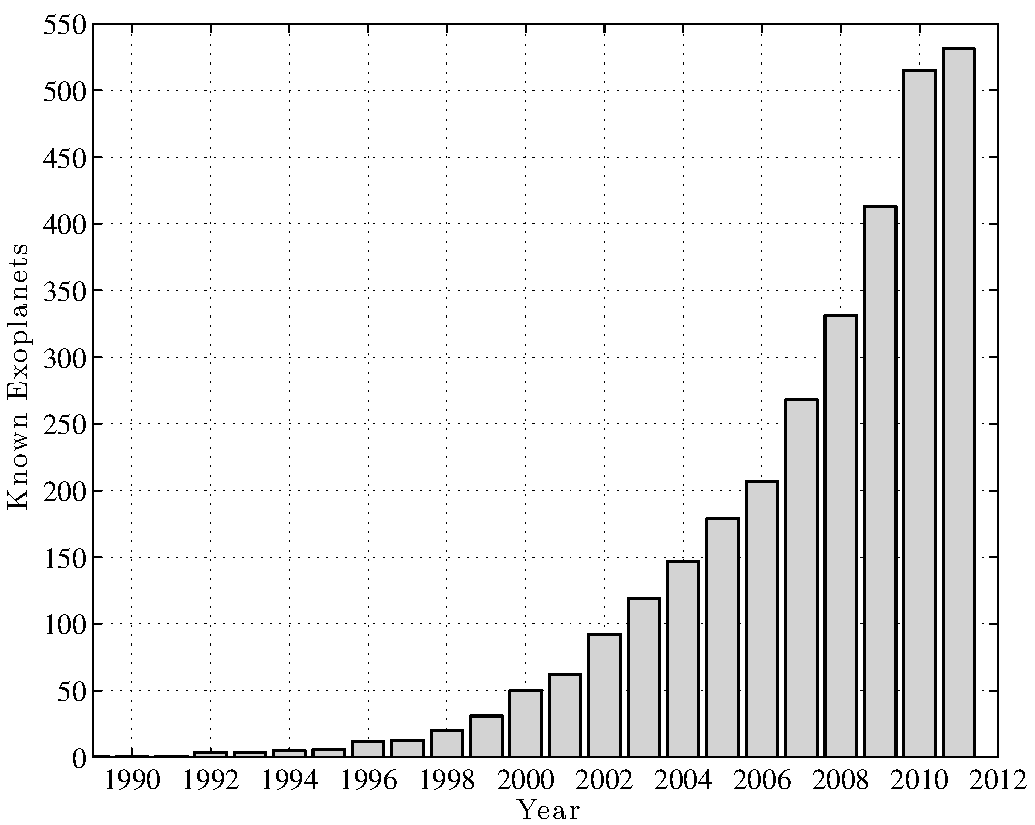
\includegraphics[width=5.5in]{./figures/planDiscHist}
  \caption[History of exoplanet discovery]{ \label{fig:planDiscHist} Number of confirmed exoplanets as a function of year.  There are currently 531 known exoplanets, and over 1200 planetary candidates.  Data retrieved from the NASA/IPAC/NExScI Star and Exoplanet Database \url{http://nsted.ipac.caltech.edu} on April 17th, 2011.}
\end{figure} 

Our ability to find large numbers of exoplanets is the key to our eventual understanding of planet formation and evolution.  To understand why, we need only look at the history of astrophysics and our knowledge of the formation and evolution of stars and galaxies.  Stellar and galactic evolution take place on time scales so vast that not even multiple generations of astronomers could hope to see many changes in the stars in our sky.  However, despite having only a static view of these dynamic processes, we are lucky enough to have an incredibly large sample of observable objects, all at various stages of development.  This large data set, along with the convenient fact that looking further into the universe is equivalent to looking further back in time, has allowed us to deduce the processes by which stars are formed, evolve, and eventually transform into a variety of other interesting objects.  We've gained confidence in these models based on our ability to locate stars at each stage of the process.  With a sufficiently large pool of observed exoplanets, we can expect the same outcome for planet science.

Unfortunately, observing exoplanets is significantly harder than observing stars.  There are no examples of bright exoplanets that can be seen with the naked eye or simple instrumentation, and so we must find each exoplanet before studying it.  In many ways, this searching for exoplanets is closer to particle physics than to traditional observational astronomy.  In each case, we search for something that may not be there, guided only by constantly evolving theory.  Similarly, both new planets and new particles are often detected indirectly, based on their effects on more easily observed objects.  Finally, both pursuits require complex dedicated equipment, which often represents the extreme borders of current technology and large investments of resources.  To answer these challenges, the exoplanet community has developed new instrumentation and data analysis methods and even whole new methods for detecting the presence of exoplanets, leading to the accelerating rate of discoveries described above. 

Alongside the various planet-finding surveys, there has been a concurrent effort to develop detailed models and simulations of observatory operations and planet observations.  These simulations serve three main purposes:  first, they allow the community to directly compare the expected scientific returns of proposed observatory and mission concepts.  Second, they can be used to optimize target selection and observation scheduling for existing facilities, while providing a controlled testing environment for data processing pipelines.  Finally, the ability to calculate the probability that a planet of a given type will be observed with a given frequency, conditional on a planet formation model, means that observations can be used to choose between competing planet evolution theories and closely estimate absolute planet frequencies. 

These applications have already been proven to be helpful in both the mission planning and the data analysis.  For example, the Kepler Mission, which has more than doubled the number of exoplanet candidates since its launch in 2009, utilizes the Kepler end-to-end model---an integrated simulation used to  test the data processing pipeline and simulate observatory operations \citep{bryson2010kepler}.  Similarly, there have been many statistical analyses of the existing exoplanet data set that relied heavily on observation modeling, including the analysis of 
radial velocity surveys in \citet{cumming2008} and a microlensing study described in \citet{gould2010frequency}.

This thesis will explore exoplanet observation modeling in relation to all of these applications.  We will start by formulating a standardized set of parameters for use throughout the rest of the chapters.  The remainder of this chapter will introduce the variables required to describe how planets orbit their parent (or host) stars and how their position and motion in space can be defined with respect to a specific observer.  We will also detail how light from stars and planets interacts with imaging systems to produce the images that form the raw data for many planet-finding methods.  

This description will be continued in \refch{ch:obs_methods} with a detailed discussion of four methods used to study exoplanets.  These are: doppler spectroscopy, which produced the majority of exoplanet detections before 2010, precision astrometry, which has the potential of allowing us to detect planets much smaller than those currently being found, transit photometry, which, thanks to the Kepler mission, has more than doubled the number of exoplanet candidates, and finally direct detection, which promises to become a very powerful tool in the near future, and has already produced a number of fascinating discoveries.  The first three of these methods, doppler spectroscopy, astrometry, and transit photometry, are indirect---they rely on observations of the star in order to infer the presence of planets, tracking the star's motion in the case of astrometry and doppler spectroscopy, and the amount of light coming from the target system in the case of transit photometry.  Direct detection is the only method that attempts to image the exoplanets themselves.  Each of these methods has specific strengths and limitations, all of which will be discussed in detail.

\refch{ch:param_dists} will review what we currently know about exoplanets, and introduce the idea of a statistical approach to exoplanet study, focusing on properties of populations of planets rather than specific examples.  Based on the formalism laid out in the first two chapters, we will develop a statistical description of planetary orbits, which will be applied to the optimization of planet-finding surveys.  In the course of this discussion we will introduce the concept of completeness, which allows for a systematic way of incorporating instrument biases into the analysis of generated data.

\refch{ch:obs_sims} will discuss the various components required to build complete simulations of exoplanet observations.  Starting with the generation of sample exoplanetary systems, we will track each step of how a realistic data set can be generated for each observation method.  We will also explore how to propagate systems forward in time so that we can simulate entire surveys in addition to individual observations.  These techniques will be applied to the construction of an integrated simulation capability for direct detection planet-finders, which will be employed in a series of case studies to explore the performance of multiple proposed missions.

Finally, \refch{ch:int_data} will consider the data analysis problem, and will demonstrate how the formalism built up throughout the thesis, along with the well-developed field of optimal estimation, can be used to systematically generate complex planetary system models from multiple varied data streams.  Taking into account the accelerating rate of discovery and the proliferation of observation methods, it is highly likely that these are the kinds of data sets the exoplanet community will have at its disposal in the near future, and the applications described in this chapter are a first step towards taking advantage of the increased information that can be extracted thanks to detailed modeling and simulation.

\section{Exosystem Parameters}\label{sec:exosystem_params}

Before proceeding, it is important to define a consistent description of all of the physical quantities that will be treated in later chapters.  This section defines every variable that will be used in multiple contexts so as to preserve a uniform notation throughout.

\begin{figure}[ht] 
 \center
 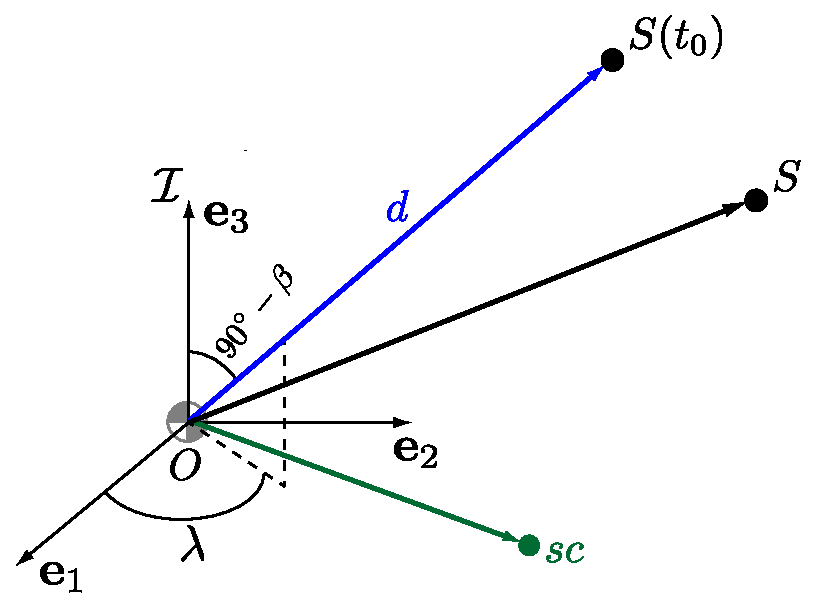
\includegraphics[width=4.5in]{./figures/barycentric_frame}
  \caption[Inertial barycentric/ecliptic frame]{ \label{fig:baryFrame} The inertial barycentric/ecliptic frame $\mc I$ with origin $O$ at the solar system barycenter.  Star $S$ is at coordinates $\lambda, \beta$ and distance $d$ at reference epoch $t_0$.}
\end{figure} 
The position of an exosystem primary star (or `target' star) is denoted by $S\addsymbol{$S$}{Star position}$, and, when expressed with respect to some specific point $P$, is given by the vector $\R_{S/P}$.  The observer location is denoted by point $sc\addsymbol{$sc$}{Observer position}$, which may represent a space or ground-based observatory.  We sometimes find it useful to define the star position via a celestial coordinate system.  Typically, we use a barycentric/ecliptic frame $\mc I = (O, \mf e_1,\mf e_2, \mf e_3)\addsymbol{$\mc I$}{Inertial barycentric/ecliptic solar system frame.}$ whose origin $O\addsymbol{$O$}{Solar system barycenter}$ is at the solar system barycenter (see \reffig{fig:baryFrame}).   In this frame, coordinates $(\lambda,\beta)$ along with the target star distance $d\addsymbol{$d$}{Star distance with respect to solar system barycenter}$ define the star position as:
\begin{equation}
\left[\R_{S/O}\right]_\mathcal{I}  =  d\left[ \begin{array}{c} \cos \lambda \cos \beta \\ \sin \lambda \cos \beta \\ \sin \beta \end{array}\right] \,,
\end{equation}
where
\begin{equation}
d \triangleq \Vert \mf r_{S/O} \Vert \,.
\end{equation}
It is important to note that $(\lambda$, $\beta)$ and $d$ are typically catalogued values, and thus define the star position at a specific epoch ($t_0$), whereas the star-pointing vector with respect to the solar system barycenter and the observer is constantly changing.

Similarly, the position of a planet is given by point $P\addsymbol{$P$}{Planet position}$ and the exosystem barycenter is defined as $G\addsymbol{$G$}{Exosystem barycenter}$.  In cases with multiple planets in one exosystem, the planet positions are enumerated as $P_i$. The star-planet separation vector is given by:
\begin{equation}
\R_{P/S} \triangleq \R_{P/G} - \R_{S/G} \,.
\end{equation}
The time varying orbital radius, $r\addsymbol{$r$}{Orbital radius}$ is equal to the magnitude of the star-planet vector:
\begin{equation}
r  \triangleq  \Vert \R_{P/S} \Vert \,.
\end{equation}
The planet's geometric albedo and radius are given by $p\addsymbol{$p$}{Geometric albedo}$  and $R\addsymbol{$R$}{Planet radius}$, respectively, and the total flux of the planet and star are given by $F_p\addsymbol{$F_p$}{Planet flux}$  and $F_s\addsymbol{$F_s$}{Star flux}$, respectively.  The intrinsic luminosity of the star is given by $L\addsymbol{$L$}{Stellar luminosity}$ measured in $L_\odot$ (solar luminosity).

It is frequently useful to describe planetary orbits via Keplerian orbital elements.  These are derived from the solution of the two-body problem, and are an exact description of planetary motion in the case of a single-planet exosystem.  In systems with multiple planets, the orbits may still be approximated as Keplerian, although this ignores all planet-planet interactions and therefore cannot exactly predict future positions of all of the system bodies.  This can still be a useful approximation, however, as no analytic solution exists to the general n-body problem.  As we will see, there are actually two different ways of approximating n-body systems via Keplerian orbital elements: we can either fit an average ellipse to multiple orbits worth of data, producing an average set of Keplerian elements, or we can calculate time-varying Keplerian elements to reflect the perturbations due to the other bodies in the system.  In the latter case, we typically use osculating Keplerian elements---i.e., the orbital elements of the Keplerian orbit tangent to the true orbit at that point in time.

The difference between constant, osculating, and averaged Keplerian orbital elements is very important as they describe very different things.  With a fixed Keplerian orbit, you can predict the position and velocity of the planet for all time.  If there are no perturbations on the planet, this position and velocity will be correct.  With perturbations, however, the true position and velocity will progressively deviate from the ones predicted by the Keplerian orbit.  An averaged set of orbital elements will never exactly match the planet's true position and velocity, but will minimize the position error over an entire data set.  Osculating orbital elements will always give you the correct position and velocity, but require knowledge of the perturbations acting on the planet.

Furthermore, while a constant set of Keplerian elements describes a particular ellipse corresponding to the planet's orbit, osculating elements are much more difficult to interpret, as they only correspond to the instantaneously tangential orbit.  This means that in certain cases the osculating orbit will be highly eccentric while the planet's orbit is actually nearly circular\footnote{This is particularly true for resonant orbits \citep{tinney20062}.}.  Throughout this thesis, we will employ both types of orbital elements.  When dealing with single planet system simulations, as in \S\ref{sec:sysProp}, we will employ constant Keplerian orbital elements.  When using orbital elements to talk about multi-planet systems, as we do later in this section, we will use osculating orbital elements.  Finally, when discussing how certain detection methods that rely on finding periodic signals to detect planets, we will employ averaged orbital elements (see \refch{ch:obs_methods} and \S\ref{sec:state_init_apri}).

\begin{figure}[ht]
 \center
 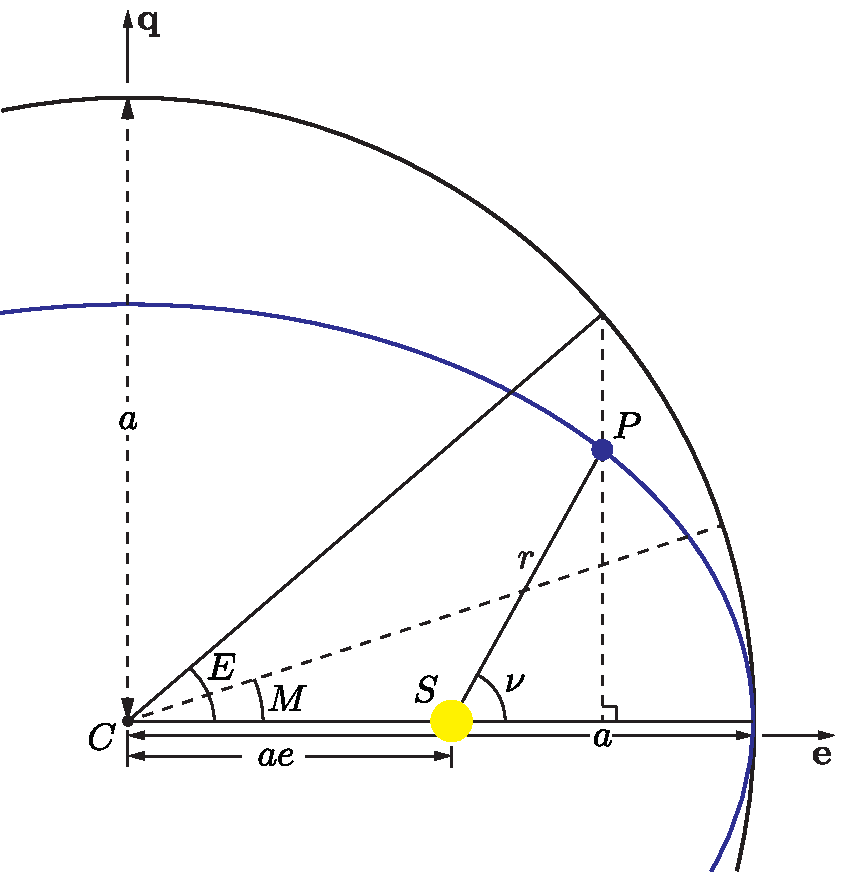
\includegraphics[width=4.5in]{./figures/anomaly_diagram}
  \caption[Anomaly Diagram]{ \label{fig:anomaly_diagram} Schematic of a Keplerian orbit (blue ellipse) and auxiliary circle (black ellipse).  The auxiliary circle has a radius equal to the orbit's semi-major axis, with center $C$.}
\end{figure} 
We define a Keplerian orbit via the parameter set $(a,e,\psi,\theta,\phi)$ where $a\addsymbol{$a$}{Orbital semi-major axis}$ is the semi-major axis, $e\addsymbol{$e$}{Orbital eccentricity}$ is the eccentricity, and $\psi,\theta,\phi\addsymbol{$\psi,\theta,\phi$}{Euler angles orienting orbit in space}$ are Euler angles determining the orientation of the orbit in the observer's reference frame\footnote{Of course, there exist many other ways of orienting the planar orbit in three dimensions.  For further discussions on some alternatives to the Euler angles, see \S\ref{sec:state_selection}.}.  The position of the planet on its orbit at the time of observation is given by either the mean anomaly $M\addsymbol{$M$}{Mean anomaly}$, eccentric anomaly $E\addsymbol{$E$}{Eccentric anomaly}$, or the true anomaly $\nu\addsymbol{$\nu$}{True anomaly}$. In a 2-body system, the planet's orbit lies in a single plane, and thus can be fully described using only scalar values, as shown in \reffig{fig:anomaly_diagram}.  Keplerian orbits are conic sections---closed planetary orbits are ellipses with the star located at one focus.  The orbital radius is defined in terms of the eccentricity, semi-major axis, and true anomaly as:
\begin{equation} \label{eq:rdef}
r = \frac{a(1-e^2)}{e \cos(\nu) + 1} \,.
\end{equation}

The orbital velocity and radius vary as functions of the true anomaly, which is defined as the angle between the current star-planet vector and the star-planet vector at the time of periapsis passage (see \reffig{fig:anomaly_diagram}).  Using the planar orbital representation, we can write the planet position and velocity  with respect to the star as:
\begin{align} 
\mf r_{P/S} &= r\left(\cos\nu \hat{\mf e} + \sin\nu \hat{\mf q}\right) \label{eq:planPosVect}\\
{}^\mc I \mf v_{P/S} &= \fddt{I} \mf  r_{P/S} = \sqrt{\frac{\mu_P + \mu_S}{\ell}}\left(-\sin\nu \hat{\mf e} + (e + \cos\nu) \hat{\mf q}\right)\label{eq:planVelVect}
\end{align}
where $\mu_P\addsymbol{$\mu_P$}{Gravitational parameter of planet}$ and $\mu_S\addsymbol{$\mu_S$}{Gravitational parameter of star}$ are the gravitational parameters of the star and planet, respectively, equal to the product of their masses ($m_S\addsymbol{$m_S$}{Mass of star}$ and $m_P\addsymbol{$m_P$}{Mass of planet}$) and the universal gravitational constant $G$.  The semi-latus rectum of the ellipse, $\ell$, is given geometrically as:
\begin{equation}\label{eq:semilatusrectum}
\ell = a(1 - e^2) \,.
\end{equation}
The unit vector $\hat{\mf e}$ (known as the normalized eccentricity vector) can be expressed as:
\begin{equation}\label{eq:eccenVec}
\hat{\mf e} = \left<\frac{1}{\mu_S + \mu_P}\left[\left( \Vert{}^\mc I \mf v_{P/S}\Vert^2 - \frac{\mu_S + \mu_P}{r}\right) \mf r_{P/S} - \left( \mf r_{P/S} \cdot {}^\mc I \mf v_{P/S}\right){}^\mc I \mf v_{P/S}\right]\right> \,.
\end{equation}
The orthogonal unit vector $\hat{\mf q}$ can be written as:
\begin{equation}\label{eq:qvecdef}
\hat{\mf q} = \left<\mf r_{P/S} \times {}^\mc I \mf v_{P/S}\right> \times \hat{\mf e}\,.
\end{equation}
These two unit vectors, $\hat{\mf e}$ and $\hat{\mf q}$, define the perifocal reference frame.  From \refeq{eq:qvecdef} we can see that the third vector of this frame, $\hat{\mf h} = \hat{\mf e} \times \hat{\mf q}$, is the direction of the orbit's normalized angular momentum:
\begin{equation} \label{eq:angMomentum}
{}^\mc I \mf h_{P/S} =  \mf r_{P/S} \times {}^\mc I \mf v_{P/S} \,,
\end{equation}
which is always orthogonal to the plane of the orbit.

To aid in calculating the planet position, it is useful to define an auxiliary circle with a radius equal to the orbit's semi-major axis and centered at the orbit's  center.  This allows us to define a mean anomaly, a central angle describing the mean planetary motion, given by:
\begin{equation} \label{eq:Mdef}
M \triangleq 2\pi \frac{t-t_p}{P_{orb}} \,,
\end{equation}
where $P_{orb}\addsymbol{$P_{orb}$}{Orbital period}$ is the orbital period, $t\addsymbol{$t$}{Time}$ is the current time, and $t_p$ is the time of the last periapsis passage (closest planet approach to the star).  The orbital period is:
\begin{equation}\label{eq:Pdef}
P_{orb} = 2\pi\sqrt{\frac{a^3}{\mu_S +\mu_P}} \,.
\end{equation}
The mean anomaly is proportional to the area covered by $\mf r_{P/S}$ since periapsis passage, and is thus linear in time.  The eccentric anomaly is related to the mean anomaly via the Kepler equation:
\begin{equation} \label{eq:EtoM}
M = E - e\sin(E) \,,
\end{equation}
and related to the true anomaly as:
\begin{equation} \label{eq:nutoE}
\tan\left(\frac{\nu}{2}\right) =\sqrt{\frac{1+e}{1-e}} \tan\left(\frac{E}{2}\right) \,.
\end{equation}

To orient the orbit in some observer's reference frame $\mc A$, we apply a 3-1-3 rotation using the angle set $(\psi,\theta,\phi)_{\mc A}$ \citep{kane}:
\begin{equation}\label{eq:rpsrot}
[\mf r_{P/S}]_{\mc A}  =
\left[ \begin{matrix} \cos\phi &\sin\phi & 0 \\ -\sin\phi& \cos\phi & 0 \\ 0 & 0 & 1 \end{matrix}\right]
\left[ \begin{matrix} 1 & 0 & 0 \\ 0 & \cos\theta &\sin\theta \\0 & -\sin\theta & \cos\theta \end{matrix}\right]
\left[ \begin{matrix} \cos\psi &\sin\psi & 0 \\ -\sin\psi & \cos\psi & 0 \\ 0 & 0 & 1 \end{matrix}\right]
[\mf r_{P/S}]_{\mc P}   \,,
\end{equation}
where $\mc P$ is a reference frame whose first two unit vectors lie in the $\hat{\mf e},  \hat{\mf q}$ plane and whose third unit vector is in the $\hat{\mf h}$ direction
(see \S\ref{sec:direct_detection} for an example of one such frame).  The  $\mc P$ frame is inertial only in the case of a non-accelerating frame origin, which results in another difficulty in using the Keplerian description as this makes $\mc P$ a heliocentric frame.  Note that we have used left-handed rotations here to conform to conventions in the literature (cf.~\citet{vinti}).  We can use these rotations to convert between the Keplerian orbital elements and the heliocentric planet position and velocity, simply by by expressing the planar orbit as:
\begin{equation}\label{eq:rpsP1}
[\mf r_{P/S}]_{\mc P}  = \left[\begin{matrix} r \cos \nu \\ r \sin \nu \\ 0 \end{matrix} \right] = \left[\begin{matrix} a (\cos E - e) \\ b \sin E \\ 0 \end{matrix} \right] \,,
\end{equation}
where $b$ is the semi-minor axis of the orbit, given by:
\begin{equation}
b = a\sqrt{1 - e} \,,
\end{equation}
and we take the angle set $(\psi,\theta,\phi) = (\Omega, I, \omega)$ where $\Omega\addsymbol{$\Omega$}{Longitude of the ascending node}$ is the longitude of the ascending node, $I\addsymbol{$I$}{Inclination}$ is the inclination and $\omega\addsymbol{$\omega$}{Argument of periapsis}$ is the argument of periapsis.  The velocity vector is found by differentiating the position, yielding:
\begin{equation}\label{eq:vpsP1}
[{}^\mc P \mf v_{P/S}]_{\mc P} = \fddt{P}{[\mf r_{P/S}]_{\mc P}} =  \sqrt{\frac{\mu_S + \mu_P}{a}}\frac{1}{1 - e\cos E} \left[\begin{matrix} -\sin E\\ \sqrt{1 - e}\cos E \\ 0 \end{matrix} \right] \,.
\end{equation}
 There are multiple algorithms for converting heliocentric position and velocity vectors to Keplerian orbital elements.  One of the most straight-forward, described in \citet{vinti}, assumes a planar orientation as in \refeq{eq:rpsrot} and then calculates the semi-major axis and semi-latus rectum from the orbital energy and angular momentum:
\begin{align}
a = -\frac{\mu_S + \mu_P}{2E} &= -\frac{\mu_S + \mu_P}{2}\left[ \frac{\Vert {}^\mc I \mf v_{P/S} \Vert^2}{2} -\frac{\mu_S + \mu_P}{\Vert \mf r_{P/S}\Vert}\right]^{-1} \,, \label{eq:vec2orbelem1} \\
\ell &= \frac{{}^\mc I \mf h_{P/S}}{\mu_S + \mu_P} \frac{\Vert  \mf r_{P/S} \times  {}^\mc I \mf v_{P/S} \Vert}{\mu_S + \mu_P} \,.
\end{align}
The eccentricity can then be calculated via \refeq{eq:semilatusrectum}:
\begin{equation}
e = \sqrt{1 - \frac{\ell}{a}} \,.
\end{equation}
Given inertial frame unit vectors $(\mf e_1, \mf e_2, \mf e_3)$, we can write:
\begin{align}
\cos I &= \frac{(\mf r_{P/S} \times  {}^\mc I \mf v_{P/S}) \cdot \mf e_3}{\Vert \mf r_{P/S} \times  {}^\mc I \mf v_{P/S}\Vert} \label{eq:cosI}\,,
\\
\sin I  &= \frac{\Vert  \mf e_3 \times (\mf r_{P/S} \times  {}^\mc I \mf v_{P/S}) \Vert}{\Vert \mf r_{P/S} \times  {}^\mc I \mf v_{P/S}\Vert} \,,
\\
\cos \Omega &= -\frac{(\mf r_{P/S} \times  {}^\mc I \mf v_{P/S}) \cdot \mf e_2}{\Vert \mf r_{P/S} \times  {}^\mc I \mf v_{P/S}\Vert \sin I} \,,
\\
\sin \Omega  &= \frac{(\mf r_{P/S} \times  {}^\mc I \mf v_{P/S}) \cdot  \mf e_1}{\Vert \mf r_{P/S} \times  {}^\mc I \mf v_{P/S}\Vert \sin I} \,,
\\
\cos \omega &= \frac{1}{e\sin I} \left(\frac{\Vert \mf r_{P/S} \times  {}^\mc I \mf v_{P/S} \Vert \left( {}^\mc I \mf v_{P/S} \cdot \mf e_3\right)}{\mu_S + \mu_P} - \frac{ \Vert \mf r_{P/S} \times  {}^\mc I \mf v_{P/S} \times \mf r_{P/S}  \Vert}{\Vert \mf r_{P/S} \times  {}^\mc I \mf v_{P/S} \Vert \Vert \mf r_{P/S} \Vert}\right) \,,
\\
\sin \omega  &= \frac{1}{e\sin I} \left(\frac{ \Vert  {}^\mc I \mf v_{P/S} \times \mf r_{P/S} \times  {}^\mc I \mf v_{P/S} \Vert}{\mu_S + \mu_P} - \frac{ \mf r_{P/S} \cdot \mf e_3}{\Vert \mf r_{P/S} \Vert}  \right) \label{eq:sinO}\, .
\end{align}
With both sine and cosine expressions for an angle, the angle may be reconstructed over the full range of $[0, 2\pi]$ with the two argument arctangent function:
\begin{equation}
\textrm{atan2}(y,x) = \left\{\begin{array}{l l}
\tan^{-1}\left(y/x\right) & x > 0\\
\pi + \tan^{-1}\left(y/x\right) & x < 0, y \ge 0\\
-\pi + \tan^{-1}\left(y/x\right) & x < 0, y < 0\\
\pi/2 & x =  0, y > 0\\
-\pi/2 & x = 0, y < 0
\end{array} \right.
\end{equation}
where $y = \cos\theta$ and $x = \sin\theta$.  Thus Equations (\ref{eq:cosI}) through (\ref{eq:sinO}) can be used to precisely orient the orbit in the unit sphere given a single measurement of the position and velocity vectors.  The time varying Keplerian orbital element (anomaly) can similarly be found by using:
\begin{align}
\cos E &= \frac{1}{e}\left(1 - \frac{\Vert \mf r_{P/S} \Vert}{a}\right) \,,\\
\sin E &= \frac{{}^\mc I \mf v_{P/S} \cdot \mf r_{P/S}}{e\sqrt{a(\mu_S + \mu_P)}} \label{eq:vec2orbelemf}\,.
\end{align}
Because this algorithm requires no iteration and the equations can be fully vectorized, the transformation can be implemented very efficiently (see \refcode{code:vec2orbElem}).

As previously mentioned, the Keplerian description is exact only for two body systems and can only be used as an approximation when a system contains more than two massive bodies (especially if the planetary bodies have substantial masses, as in cases of systems with multiple Jupiter-size planets).  A much more exact approximation of the motion of n bodies utilises Newton's law of gravity to express the dynamics of the planetary system via the second-order, ordinary differential equation:
\begin{equation}\label{eq:nbody}
\fdddt{I}{\mf r_{j/O}} = \sum_{k\in Y}\mu_k \frac{\mf r_{k/O} - \mf r_{j/O}}{\Vert \mf r_{k/O} - \mf r_{j/O}\Vert^3}\,, \, j \in X
\end{equation}
where the set $X$ contains all of the bodies in the system:
\begin{equation} \label{eq:Xsetdef}
X = \left\{P_1, P_2,\ldots,P_n,S\right\} \,,
\end{equation}
while the $Y$ is the subset of $X$ not containing $j$:
\begin{equation}
Y \subset X : j \notin Y \,.
\end{equation}
The total energy, which is conserved in the absence of external perturbations, can be expressed as:
\begin{equation}\label{eq:Etot}
E_{tot} = \sum_{j \in X} \left(\frac{m_j}{2}\left({}^I \mf v_{j/O} \cdot {}^I \mf v_{j/O}\right) - \sum_{k \in Y} \frac{m_j\mu_k}{\Vert \mf r_{k/O} - \mf r_{j/O}\Vert}\right) \,. 
\end{equation} 

\begin{figure}[ht]
 \center
 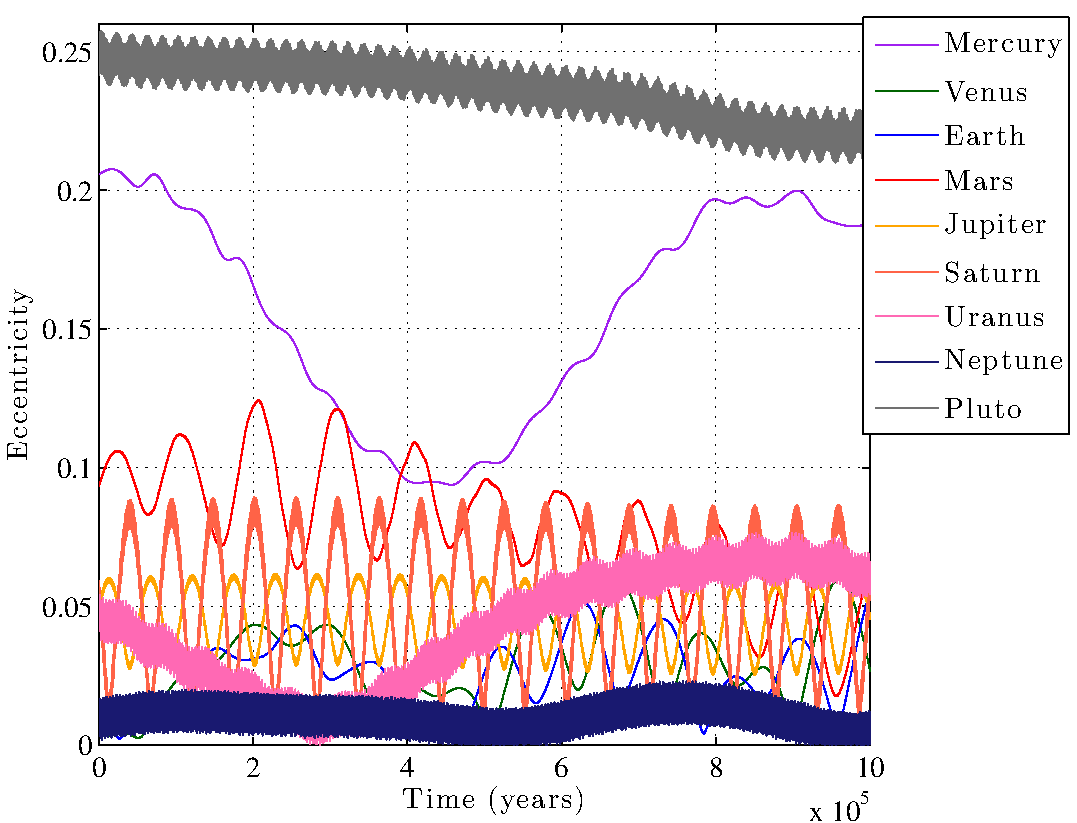
\includegraphics[width=6in]{./figures/eccenVar}
  \caption[Eccentricity variation]{ \label{fig:eccenVar} Variation in orbital eccentricities of solar system bodies over one million years.}
\end{figure}
In the case where there are only two bodies (say, a star and one planet), \refeq{eq:nbody} can be rewritten in terms of the separation vector between the pair, rather than with respect to some inertial origin:
\begin{equation}\label{eq:twoBody}
\fdddt{I}{\mf r_{P/S}} + (\mu_S + \mu_P) \frac{\mf r_{P/S}}{\Vert\mf r_{P/S}\Vert^3} = 0 \,,
\end{equation}
from which all of Kepler's laws and orbital equations can be derived.  Using Equations (\ref{eq:vec2orbelem1}) through (\ref{eq:vec2orbelemf}), we can see that in the multi-planet case, the Keplerian orbital elements represent instantaneous fits to \refeq{eq:twoBody}, which approximates the true system dynamics assuming that the combined effects due to all other bodies in the system are small compared to those due to the star.  Alternatively, we can find osculating Keplerian elements for multi-body systems that are time-varying, as in \reffig{fig:eccenVar}.
 
Of course, the Newtonian formulation is itself an approximation, with the true expressions for the motions of bodies in gravitational fields given by the Einstein field equations.  There are almost no cases in the modeling of planetary systems where it is necessary to use the field equations to calculate the exact metric tensor, but there may be observable general relativity effects in bodies orbiting closely to their parent stars (as happens, for example, with Mercury in our solar system \citep{fabrycky2010non}).  In these cases, it is possible to model some of the `post-Newtonian' effects by expanding the field equations to first order in the ratio of orbital velocity and the speed of light.  One example of this is the Einstein-Infeld-Hofmann equations of motion \citep{einstein1938gravitational,einstein1940gravitational}:
\begin{align}
\fdddt{I}{\mf r_{j/O}} = &\sum_{k\in Y} \frac{\mu_k(\mf r_{k/O} - \mf r_{j/O})}{\Vert \mf r_{k/O} - \mf r_{j/O}\Vert^3} 
+ \frac{1}{c^2}\sum_{k\in Y} \frac{\mu_k(\mf r_{k/O} - \mf r_{j/O})}{\Vert \mf r_{k/O} - \mf r_{j/O}\Vert^3}\left[  {}^I \mf v_{j/O} \cdot {}^I \mf v_{j/O} \phantom{\fdddt{I}{\mf r_{k/O}}}\right. \nonumber\\
&{} + 2 {}^I \mf v_{k/O} \cdot {}^I \mf v_{k/O} - 4 {}^I \mf v_{j/O} \cdot {}^I \mf v_{k/O} - \frac{3}{2}\left(\frac{(\mf r_{j/O} - \mf r_{k/O}) \cdot {}^I \mf v_{k/O} }{\Vert \mf r_{j/O} - \mf r_{k/O} \Vert}\right)^2 \nonumber\\
&\left. {} - 4\sum_{i \in Y} \frac{\mu_i}{\Vert \mf r_{j/O} - \mf r_{i/O}\Vert} - \sum_{i \in Z}\frac{\mu_i}{\Vert \mf r_{k/O} - \mf r_{i/O}\Vert} + \frac{1}{2}\left((\mf r_{k/O} - \mf r_{j/O})\cdot \fdddt{I}{\mf r_{k/O}}\right)\right] \nonumber \\
&{}+ \frac{1}{c^2}\sum_{k\in Y} \frac{\mu_k}{\Vert \mf r_{k/O} - \mf r_{j/O}\Vert^3}\left[ (\mf r_{j/O} -\mf r_{k/O} )\cdot (4 {}^I \mf v_{j/O} - 3  {}^I \mf v_{k/O} )\right] ( {}^I \mf v_{j/O}-  {}^I \mf v_{k/O} ) \nonumber \\
&{} + \frac{7}{2c^2} \sum_{k\in Y} \frac{\mu_k}{\Vert \mf r_{k/O} - \mf r_{j/O}\Vert}\fdddt{I}{\mf r_{k/O}}\,, \, j \in X \label{eq:einstein_nbody}
\end{align}
where  $c\addsymbol{$c$}{Speed of light}$ is the speed of light and $Z$ is the subset of $X$ not containing $k$:
\begin{equation}
Z \subset X : k \notin Z \,.
\end{equation}
Besides being functionally more complex than \refeq{eq:nbody}, this equation is also significantly more difficult to integrate as it contains velocity terms (invalidating a whole class of second-order integrators that are commonly used to integrate n-body systems) as well as acceleration terms, which require a fully implicit integrator.  Because of this, it is common practice to integrate only the Newtonian formulation, and to apply the post-Newtonian correction only when deviations due to general relativity effects become too pronounced to ignore\footnote{For further discussion on numerical integration see \S\ref{sec:gen_plan_sys}.}.

\section{The Point Spread Function}\label{sec:PSF}
Before proceeding to any discussion of specific detection methods, we need a standardized description of an imaging system, which will be used to develop the models for direct detection, doppler spectroscopy, and transit photometry (and is also applicable to some interferometers used for astrometry).  Following \citet{goodman2005introduction}, we assume the imaging system to act as a linear operator $\mc F$ such that,
\begin{equation}
\mc F: E_o(u,v) \rightarrow E_i(x,y)
\end{equation}
where $E_o(u,v)$ is the electric field transmitted by the object and $E_i(x,y)$ is the image electric field (with image coordinates $x,y$).  The input can be decomposed by taking advantage of the Dirac $\delta$ function as:
\begin{equation}
E_o(u,v) = \iint\limits_{-\infty}^{\quad \infty} E_o(\xi,\eta) \delta(u-\xi, v-\eta) \intd{\xi}\intd{\eta} \,,
\end{equation}
so that we can write:
\begin{equation}\label{eq:supInt}
E_i(x,y) = \iint\limits_{-\infty}^{\quad \infty} E_o(\xi,\eta) h(x,y,\xi,\eta) \intd{\xi}\intd{\eta} \,,
\end{equation}
where 
\begin{equation}
h(x,y,\xi,\eta)  = \mc F\left\{ \delta(u-\xi, v-\eta) \right\} \,.
\end{equation}
The superposition integral in \refeq{eq:supInt} can be used to characterize an imaging system by its response to unit impulses via the impulse response function $h$, known as the point spread function (PSF$\addsymbol{PSF}{Point spread function}$).  This function can be interpreted as the resulting image of an electric field emitted by a point source; any image can thus be built up from images of point sources distributed throughout the field of view.  With some assumptions, it can be shown that the function $\mc F$ is a Fourier transform, allowing us to express $h$ in terms of specific instrument properties \citep{hecht2002optics,bracewell2000fourier}.

Starting with an aperture $A$ in the $(u,v)$ plane, we form another plane $(x,y)$, a distance $z$ away.  By the Huygens-Fresnel principle,
\begin{equation}
E_z(x,y) = \frac{1}{i\lambda}  \iint\limits_{A(u,v)} E_o(u,v) e^{i\frac{2 \pi}{\lambda}\Vert \mf r \Vert} \frac{\cos\theta}{\Vert \mf r \Vert}  \intd{u}\intd{v}
\end{equation}
where $\lambda\addsymbol{$\lambda$}{Wavelength}$ is the wavelength, $\mf r$ is the vector between the point in $(x,y)$ and the point in $(u,v)$, and $\theta$ is the angle between $\mf r$ and the vector normal to the two planes, such that $\cos\theta = z/\Vert \mf r\Vert$.  This formulation is based on scalar diffraction theory and assumes that $\Vert \mf r\Vert \gg \lambda$, i.e., that the image is many wavelengths from the aperture.

Applying the binomial expansion to the magnitude of $\mf r$, we have:
\begin{align}
\Vert \mf r \Vert &= z\sqrt{1 + \left(\frac{x-u}{z}\right)^2 + \left(\frac{y-v}{z}\right)^2}\\
& = z + \frac{z}{2}\left(\frac{x-u}{z}\right)^2+ \frac{z}{2} \left(\frac{y-v}{z}\right)^2 + \cdots
\end{align}
so we make the approximation:
\begin{equation} \label{eq:fresnelint}
E_z(x,y) \approx \frac{e^{i\frac{2\pi}{\lambda}z}}{i\lambda z}  \iint\limits_{A(u,v)} E_o(u,v) e^{i\frac{\pi}{\lambda z}\left[ (x - u)^2 + (y - v)^2\right]} \intd{u}\intd{v} \,.
\end{equation}
This expression, known as the Fresnel integral, can be seen to be a convolution\footnote{Strictly, the integral should be written with limits from $-\infty$ to $\infty$, in which case it is understood that $E_o(u,v)$ is zero outside of $A(u,v)$.}  between $E_o(u,v)$ and the kernel:
\begin{equation}
h(x,y) = \frac{e^{i\frac{2\pi}{\lambda}z}}{i\lambda z}e^{i\frac{\pi}{\lambda z}\left(x^2 + y^2\right)} \,.
\end{equation}
Because this is a Gaussian Kernel, the Fourier conjugate of $E_z$ can be written as:
\begin{equation}\label{eq:fourierConj}
\hat{E}_z(\xi,\eta) = e^{i\frac{2\pi}{\lambda}z} \hat{E}_o(\xi,\eta)e^{-i\pi \lambda z\left(\xi^2 + \eta^2\right)} \,.
\end{equation}
Similarly, \refeq{eq:fresnelint} can be rewritten as:
\begin{equation}\label{eq:fresnelint2}
E_z(x,y) = \frac{e^{i\frac{2\pi}{\lambda}z}}{i\lambda z}e^{i\frac{\pi}{\lambda z}\left(x^2 + y^2\right)} \iint\limits_{-\infty}^{\quad \infty} E_o(u,v)e^{i\frac{\pi}{\lambda z}\left(u^2 + v^2\right)}  e^{-i\frac{2\pi}{\lambda z}\left(xu +yv\right)} \intd{u}\intd{v} \,,
\end{equation}
which is a scaled Fourier transform of $E_o(u,v)e^{i\frac{\pi}{\lambda z}\left(u^2 + v^2\right)}$.

Assuming that there is a lens at the aperture plane with focal length $f$, \refeq{eq:fresnelint} can be used to express the field at the focal plane as:
\begin{equation}\label{eq:lensFourierTrans}
E_f(x,y) = \frac{e^{i\frac{2\pi}{\lambda}f}}{i\lambda f}e^{i\frac{\pi}{\lambda z}\left(x^2 + y^2\right)} \hat{E}_A\left(\frac{x}{\lambda f}, \frac{y}{\lambda f}\right)
\end{equation}
for
\begin{equation}
E_o(u,v) = E_A(u,v)e^{i\frac{\pi}{\lambda f}\left(u^2 + v^2\right)} \,. 
\end{equation}
Now, if the free space propagation before the lens is equal to $f$, then Equations (\ref{eq:lensFourierTrans}) and (\ref{eq:fourierConj}) combine to produce:
\begin{equation}
E_i(x,y) = \frac{1}{i\lambda f}e^{i\frac{\pi}{\lambda f}\left( \frac{1}{f} - \frac{1}{f}\right)\left(x^2 + y^2\right)} \hat{E}_o\left(\frac{x}{\lambda f}, \frac{y}{\lambda f}\right) =  \frac{1}{i\lambda f} \hat{E}_o\left(\frac{x}{\lambda f}, \frac{y}{\lambda f}\right)
\end{equation}
so that the electric field at the focal plane is simply the Fourier transform of the incoming field.

Returning to \refeq{eq:supInt}, the impulse response function can now be written as:
\begin{equation}
h(x,y) = \frac{1}{\lambda f} \iint\limits_{-\infty}^{\quad \infty} A(u,v) e^{-i\frac{2\pi}{\lambda f}\left(xu +yv\right)} \intd{u}\intd{v} \,.
\end{equation}
Since the effect of a lens is to take the Fourier transform of the incoming field, the intensity distribution of the image is given by
\begin{equation}
I_i(x,y) = \vert \hat{E}_0\vert^2 \,,
\end{equation}
and so we can write
\begin{equation}
I_i(x,y) = \kappa \iint\limits_{-\infty}^{\quad \infty} \vert h(\xi - u, v-\eta) \vert^2 I_o(u,v) \intd{u}\intd{v} \,,
\end{equation}
for real constant $\kappa$.
We can thus define the intensity impulse response, $\vert h\vert^2$, or point spread function:
\begin{equation}\label{eq:PSFdef}
\PSF (x,y) = \frac{1}{\lambda^2 f^2} \left\vert\iint\limits_{-\infty}^{\quad \infty} A(u,v) e^{-i\frac{2\pi}{\lambda f}\left(xu +yv\right)} \intd{u}\intd{v} \right\vert^2 \,.
\end{equation}
\refeq{eq:PSFdef} provides us with a way of characterizing the effects of the optical system, and thereby the ability to disentangle these from the true signal being measured.

\bigskip
\bigskip

The descriptions of planetary orbits, physical parameters and imaging systems laid out in the previous two sections make it possible to rigorously define exactly how the different detection methods find and observe planets, using a unified syntax which will prove very important in subsequent chapters.  In the next chapter, we will introduce the four detection method studied in this thesis and, using the groundwork laid here, we will be able to describe what form the data from each detection method will take, and develop expressions for the observables and constraints of each method. 



 






 % Intro/Background
\chapter{Observation Methods}\label{ch:obs_methods}

This chapter will describe four methods currently in use for the detection of exoplanets.  While these do not represent all of the ways that have been proposed or successfully employed to study exoplanets, three of these (doppler spectroscopy, transit photometry, and astrometry) have provided us with the bulk of the currently known exoplanets, while direct detection promises to be a very powerful tool for future exoplanet study, and a subject of much interest in the community.  These four methods also fit well into the common parameter set described in \S\ref{sec:exosystem_params}, which makes it simpler to discuss applications incorporating data derived from more than one of these methods.


\section{Direct Detection}\label{sec:direct_detection}

Direct detection (or imaging) instrumentation can be split roughly into two classes: internal coronagraphs and external occulters.  Broadly speaking, internal coronagraphs seek to create regions of high contrast in the image plane by generating specialized PSFs.  This is achieved with various combinations of shaped pupils \citep{vanderbei2004checkerboard, vanderbei2003circularly, kasdin2005}, apodized pupils \citep{jacquinot1964progress, nisenson2001detection}, Lyot stops \citep{kuchner2002coronagraph, soummer2004apodized}, pupil mapping systems \citep{guyon2003,vanderbei2006diffraction}, etc. As these systems are highly sensitive to minute surface errors on any of the optical elements, they often include deformable mirrors (DMs) as part of active wave-front control systems to correct for any errors introduced in the wavefront by internal optics \citep{pueyo2008broadband}.  This adds a great deal of complexity to these systems and requires precise wavefront estimation and broadband wavefront correction, both of which are extremely difficult \citep{groff2010progress}.

\begin{figure}[ht]
 \center
 
\includegraphics[width=3in]{./figures/theiaOcculter}
  \caption[Starshade]{ \label{fig:theiaOcculter} A starshade.  The `petals' are designed to prevent diffraction of light about the central disk, thereby creating a dark region at the aperture of the telescope.}
 \end{figure}
Alternatively, external coronagraphs use a separate spacecraft (an `occulter' or `starshade'; see \reffig{fig:theiaOcculter}) between the target and the telescope to block most of the starlight from entering the telescope pupil \citep{cash2006detection,vanderbei2007,cady2010design}.  This means that the telescope itself can be fairly conventional, as the contrast level in the image plane no longer needs to be large to detect planets.  This also means that 
active wavefront control is not required, as the system is no longer highly sensitive to small errors in the optical surfaces.  However, the occulter must be flown in exact formation with the telescope throughout observations, at separations of tens of thousands of kilometers and required alignment precisions of tens of centimeters, yielding a very difficult control problem \citep{sirbu2010dynamical}.  The starshade must also be manufactured to very strict tolerances \citep{shaklan2010error}.  The modeling of a direct planetary observation will follow the descriptions in  \citet{brown2005} and \citet{savransky2010}, and will be applicable to both types of imaging systems.  

\subsection{Imaging Observables and Constraints}\label{sec:imag_inst_obs}
An observation of a planet in reflected or emitted light produces two pieces of information: the planet's position and brightness.  In most cases, these values will be relative to the primary star, providing us with the planet's position relative to the star in the plane of the sky (with respect to the observer) and the ratio of fluxes between the planet and star.  This makes it useful to define a `sky' frame,  $\mc S = (S,\mf s_1, \mf s_2, \mf s_3)\addsymbol{$\mc S$}{Sky frame}$ where the the observer line of sight to the target star is along $\mf s_3$, and the plane of the sky (from the viewpoint of the observer) lies in $(\mf s_1, \mf s_2)$.  That is, 
\begin{equation}
\frac{\mf r_{S/sc}}{\Vert \mf r_{S/sc}\Vert} \equiv \mf s_3 \,,
\end{equation}
as shown in Figure \ref{fig:orbit_diagram}.  In contrast to \refeq{eq:rpsP1}, we begin with the planar orbit orientation in $(\mf s_2, \mf s_3)$:
\begin{equation}
[\mf r_{P/S}]_{\mc P} = \left[ \begin{matrix} 0 \\ r\sin\nu \\r\cos\nu \end{matrix}\right] \,.
\end{equation}
Since the 3-1-3 rotation can orient the orbit in all directions throughout the unit sphere, the initial orientation can be in any plane.  The $(\mf s_2, \mf s_3)$ plane is used here to conform to earlier studies and allow simpler comparison of the results.  Following \refeq{eq:rpsrot}, we use the Euler angle set $(\psi,\theta,\phi)_{\mc S}$ to write:
\begin{equation}\label{eq:rpsdef}
[\mf r_{P/S}]_{\mc S}
= \left[
\begin{array}{c} r (\cos\nu  \sin\theta  \sin\phi +\sin\nu  (\cos\theta  \cos\psi  \sin\phi +\cos\phi
 \sin\psi )) \\
 r (\cos\nu  \cos\phi  \sin\theta +\sin\nu  (\cos\theta  \cos\phi  \cos\psi -\sin\phi
 \sin\psi )) \\
 r (\cos\theta  \cos\nu -\cos\psi  \sin\theta  \sin\nu )
\end{array}
\right] \,.
\end{equation}

\begin{figure}[ht]
 \center
 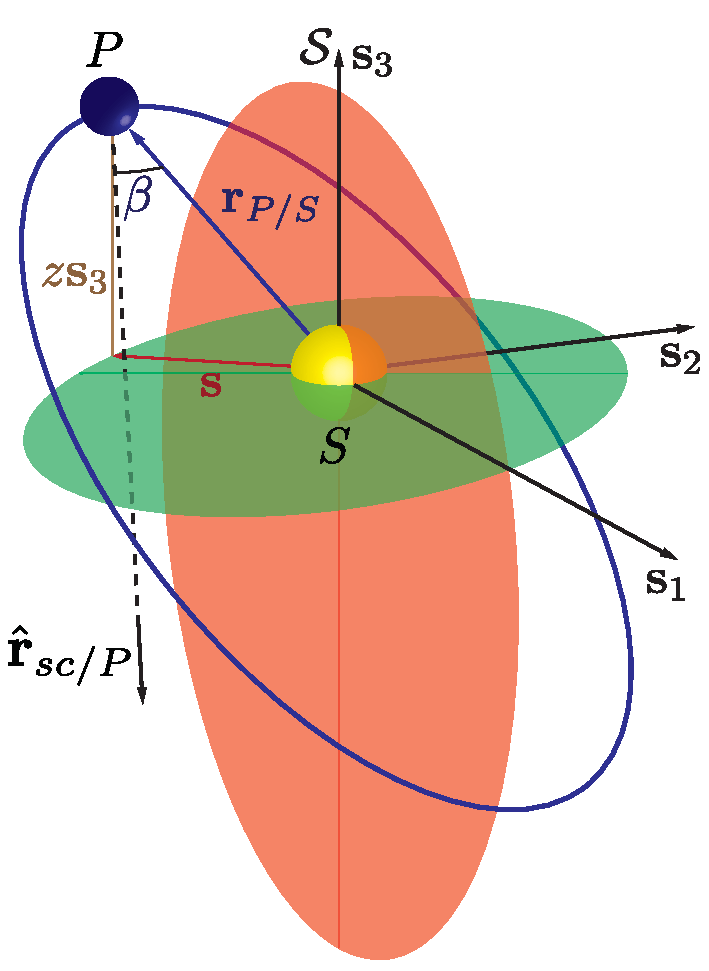
\includegraphics[width=3in]{./figures/orbit_diagram}
  \caption[Orbit Diagram]{ \label{fig:orbit_diagram} Schematic of a planetary orbit.  The green shaded ellipse represents the projection of the orbit into the plane of the sky ($\mf s_1$, $\mf s_2$), while the red shaded ellipse represents the planar orbit in ($\mf s_2$, $\mf s_3$).}
 \end{figure}
We define the separation $\mf s \addsymbol{$\mf s$}{Sky star-planet vector}$ as the projection of the star-planet vector into the plane of the sky:
\begin{equation}\label{eq:svdef}
[\mf s]_{\mc S} = \left[\begin{array}{ccc}1 & 0 & 0 \\ 0 & 1 & 0 \\ 0 & 0 & 0\end{array}\right] [\R_{p/s}]_{\mc S} \, ,
\end{equation}
as in Figure \ref{fig:orbit_diagram}.   This projection also leads us to define the apparent separation - the magnitude of the star-planet vector projected into the plane of the sky:
\begin{equation}\label{eq:sdef} \addsymbol{$s$}{Apparent separation} 
s = \Vert \mf s \Vert \,.
\end{equation}
The apparent separation may be either a derived quantity (when the instrument is capable of resolving the star-planet separation in two dimensions, or can measure the absolute planet position with respect to another reference like the solar system barycenter) or a primary observable (when the instrument can only measure the separation in one dimension).

The relative flux between the planet and its parent star is a function of the orbital radius and the planet's albedo and radius:
\begin{equation} \label{eq:fluxRatiodef}  \addsymbol{$F_R$}{Ratio of planet to star fluxes}
F_R \triangleq \frac{F_p}{F_s} = p\Phi(\beta) \left(\frac{R}{r}\right)^2 \, ,
\end{equation}
where $\Phi\addsymbol{$\Phi$}{Planet phase function}$  is the planet's phase function \citep{sobolev}, and $\beta\addsymbol{$\beta$}{Phase angle}$  is the star-planet-observer (phase) angle, given by:
\begin{equation}  
\beta = \cos^{-1}\left(\frac{\mf r_{P/sc} \cdot  \mf r_{P/S} }{\Vert \mf r_{P/sc} \Vert  \Vert\mf r_{P/S}\Vert}\right) \, ,
\end{equation}
where $\R_{P/sc}$ is the position of the planet relative to the observer:
\begin{equation}
\Vert \mf r_{P/sc} - \mf r_{sc/O} - \mf r_{P/S}\Vert = d \, .
\end{equation}
However, since $d \gg r $, we can make the approximation:
\begin{equation}  \label{eq:betadef}
\beta \approx \cos^{-1}\left(\frac{z}{r}\right) \, .
\end{equation}
where $z$ is the $\mf s_3$ axis component of $[\mf r_{p/s}]_{\mc S}$.  For the closest star to Earth (approximately 1.3 pc away), this approximation produces errors of less than 0.001\%.  The flux ratio is often expressed on a logarithmic scale, in which case it becomes the difference in magnitude between the star and planet:
\begin{equation}\label{eq:deltamagdef} \addsymbol{$\Delta$mag}{Difference in magnitude between star and planet}
\Delta\textrm{mag} \triangleq -2.5\log_{10}F_R \,.
\end{equation}

Observable limits on $s$ and $F_R$, or functions thereof, can be mapped to instrument specifications for a fairly broad variety of direct imaging instruments by assuming that a planet will be observable if its angular separation from the star is greater than the observatory's inner working angle (IWA)$\addsymbol{IWA}{Inner working angle}$, and illuminated such that the $\Delta$mag is below a threshold value, called the limiting $\Delta$mag, or $\Delta$mag$_0\addsymbol{$\Delta$mag$_0$}{Limiting $\Delta$mag}$.  The IWA represents the minimum angular separation between the telescope's central axis (line of sight) and detectable objects on the sky.  The specific determination of the IWA depends on the instrument design, and may be affected by the size of a central obscuration, the capability of an adaptive optics systems to remove light from certain areas of the image plane, or the size and geometry of external occulting optics.  

The limiting $\Delta$mag represents the point where systematic errors produce unresolvable confusion between planet signal and background noise \citep{brown2005}.   It is important to note that while this value is often equated with the designed contrast of an instrument (i.e., the ratio of the core to halo of a coronagraph's point spread function), they are not necessarily the same.  Depending on the nature of the background and instrument systematics, $\Delta$mag$_0$ may actually be less than the designed contrast.  In fact, it is becoming standard practice to set the design contrast at several magnitudes below the $\Delta$mag$_0$ required by the population of interest, based on a detailed error budget (see, for example, \citet{shaklan2010error}).  \reffig{fig:imagingConstraintsSchem} shows a schematic of the instrument constraints on direct imaging.
\begin{figure}[ht]
 \center
 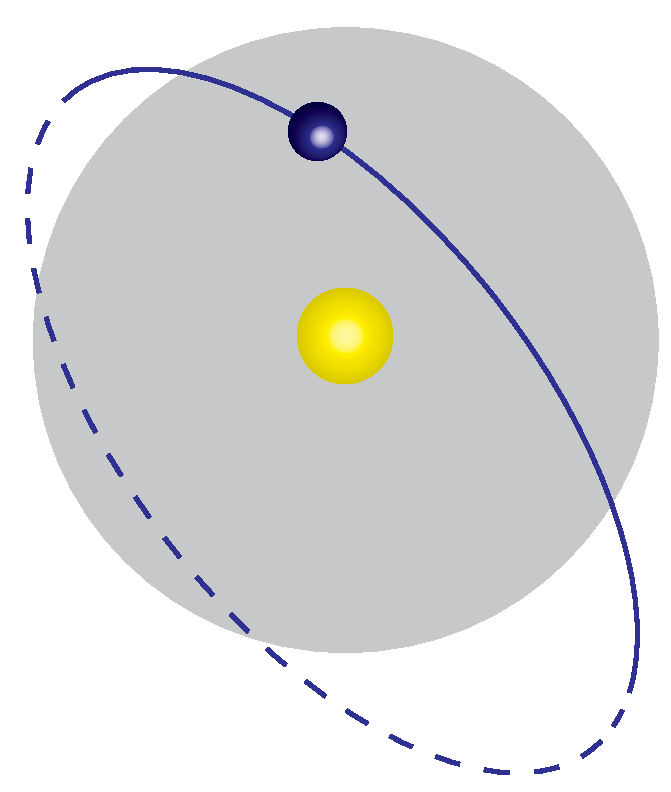
\includegraphics[width=3in]{./figures/imagingConstraintsSchem}
  \caption[Imaging constraints diagram]{ \label{fig:imagingConstraintsSchem} Schematic of the instrument constraints on direct imaging.  The shaded circle centered on the star represents the projected IWA (no observations can be made within this angle of the star) and the planet is sufficiently illuminated ($\Delta$mag  < $\Delta$mag$_0$) on the solid portion of the orbit (when the planet is between the observer and the star along the line of sight).  In this case, the planet is only observable on two small portions of its orbit near periapsis and apoapsis.}
 \end{figure}

A significant difference between occulters and coronagraphs is the dependence of their IWA on wavelength.  The extent of the coronagraph's produced region of high contrast depends completely on the geometry of the internal optics.  If the region extends to some location $n$ in the image plane, then it represents an aperture plane location of $n/f \lambda/D$ where $D$ is the aperture diameter and $f$ is the focal length.  Thus, the IWA for the coronagraph is commonly given in units of $\lambda/D$, and changes with wavelength.  An occulter, on the other hand creates a region of high contrast over a specific wavelength band.  In this case, the light from the star is removed before it ever gets to the telescope, so the dark region extends throughout the entire image plane.  On the other hand, if the angular separation of the planet from the star is less than the angular size of the occulter on the sky, then the light from the planet will also be blocked.  Therefore, the IWA (often called the geometric IWA) for the occulter is set by its radius $R_O$ and separation distance from the telescope $d_s\addsymbol{$d_s$}{Occulter separation distance}$:
\begin{equation}
\textrm{IWA}_\textrm{geom} = \sin^{-1}\left(\frac{R_O}{d_s}\right) \,.
\end{equation}
Because occulters are designed with petals (as in \reffig{fig:theiaOcculter}), it is actually possible to see some of the planet light coming through the gaps between the petals when the planet is inside the geometric IWA, albeit at a significantly decreased system throughput.

\begin{figure}[ht]
 \center
 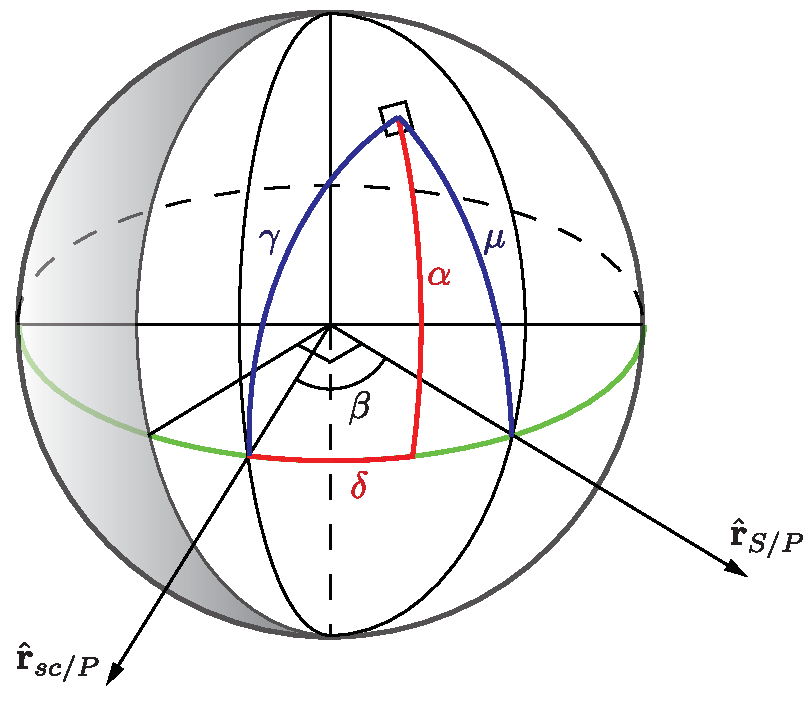
\includegraphics[width=4in]{./figures/reflection_diagram}
  \caption[Reflection Diagram]{ \label{fig:reflection_diagram} Schematic of a reflecting spherical body.  The angles $(\alpha, \delta)$ are the coordinates of an arbitrary point on the surface, $\mu$ is the angle of incident radiation, and $\gamma$ is the angle of emergent radiation.}
 \end{figure}
 We have so far defined all of the elements that are used to calculated $s$ and $F_R$, except for the phase function.  Unfortunately, there can be no single definition for $\Phi$, as it depends on the characteristics of a given planet.  One way to get around this difficulty is to assume that the planet can be modeled as a Lambertian reflector, i.e., that the planet's surface luminance is isotropic.  This leads to the commonly used Lambert phase function.  Because of the importance of this function, it is useful to briefly derive it here.  Following \citet{sobolev}, we let $(\alpha, \delta)$ be the planetary latitude and longitude of an arbitrary point on the planet's surface, $\mu$ the angle of incident radiation, $\gamma$ the angle of emergent radiation at a surface point, and $\xi$ the azimuthal angle between $\mu$ and $\gamma$ such that:
\begin{equation}
\cos \xi = \frac{\cos\mu\cos\gamma - \cos\beta}{\sin\mu\sin\gamma} \,.
\end{equation}
These definitions are shown schematically in \reffig{fig:reflection_diagram} and yield the realtionships:
\begin{align}
	\cos\mu &= \cos\alpha \cos(\beta - \delta) \triangleq C_\mu \,,\\
	\cos\gamma &= \cos\alpha \cos\delta \triangleq C_\gamma \,.
\end{align}
	
The emergent intensity is given by:
\begin{equation}
I = C_\gamma F \rho(C_\mu,C_\gamma,\xi) \,,
\end{equation}
where $\pi C_\gamma F$ is the flux on a patch of the surface and $\rho$ is the reflection coefficient.  The energy crossing a surface patch into unit solid angle is $C_\gamma C_\mu F \rho \intd{A}$ where
\begin{equation}
\mathrm{d}A = R^2 \cos\alpha \intd{\alpha} \intd{\delta} \,.
\end{equation}
The energy per second per unit area per unit solid angle received by an observer is thus:
\begin{equation}
E(\beta) = \frac{F R^2}{r^2} \int_{\beta - \pi/2}^{\pi/2} \cos(\beta - \delta) \cos\delta \intd{\delta}  \int_{-\pi/2}^{\pi/2} \rho(C_\mu,C_\gamma,\xi) \cos^3 \alpha \intd{\alpha}
\end{equation}
The phase function is defined as the ratio of $E(\beta)/E(0)$.  For isotropic scattering, $\rho$ is constant so:
\begin{equation}\label{eq:lambertPhaseFunc}
\Phi_L(\beta) = \frac{\int_{\beta - \pi/2}^{\pi/2} \cos(\beta - \delta) \cos\delta \intd{\delta}}{ \int_{-\pi/2}^{\pi/2} \cos(-\delta) \cos\delta \intd{\delta}} = \frac{\sin(\beta)+(\pi-\beta)\cos(\beta)}{\pi}
\end{equation}

\begin{figure}[ht]
 \center
 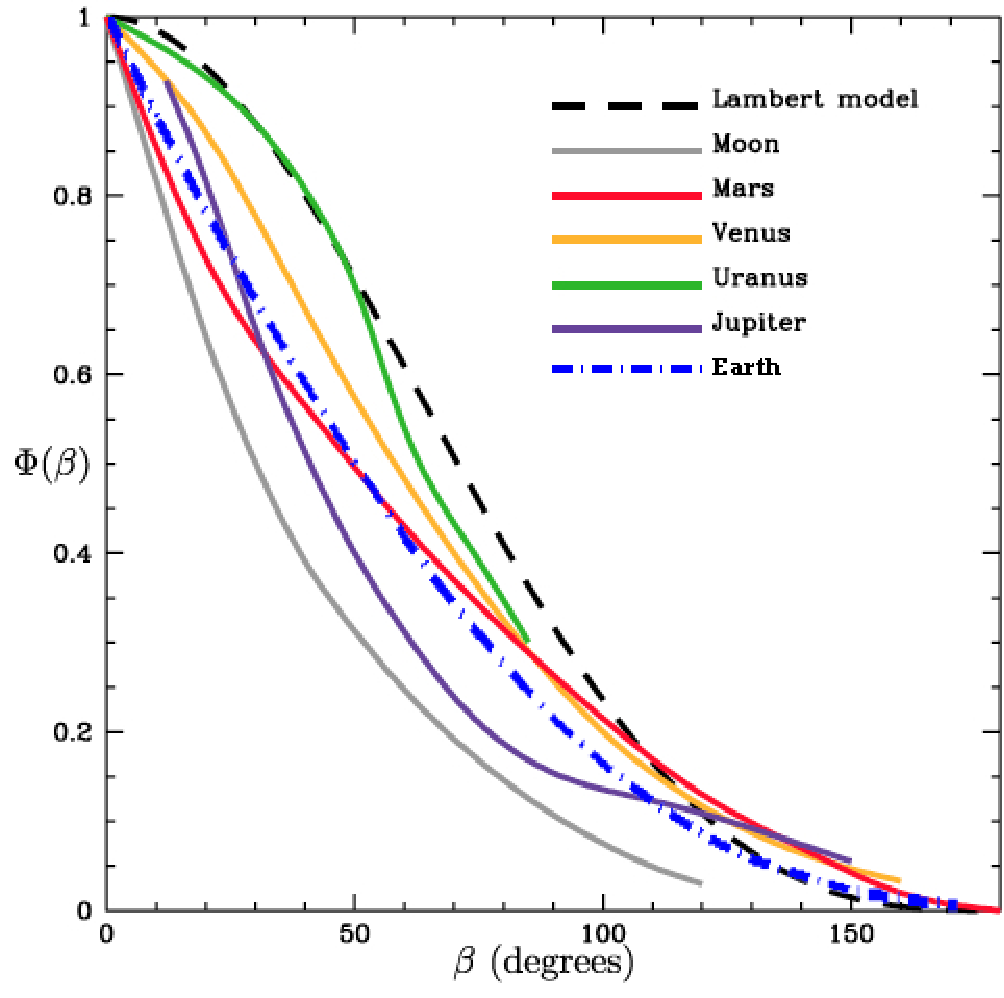
\includegraphics[width=4.5in]{./figures/phi_v_beta}
  \caption[Solar system planet phase functions]{ \label{fig:phi_v_beta} Empirically determined phase functions of solar system bodies plotted with the Lambert phase function.  Data from \citet{sudarsky2005} and \citet{devaucouleurs1964geometric}.}
 \end{figure}
Figure \ref{fig:phi_v_beta} compares the Lambert phase function with empirical values found for the various planetary bodies in the solar system.  It is immediately evident that the assumption of isotropic scattering is not a good one for most of these, as it overestimates the true phase function in almost all cases.  More precise modeling can be achieved by using empirically derived lookup tables, whenever possible.

Having a functional form for the phase function does have certain advantages, however.  For example, we can quantify the relationships between the direct detection observables such as the extrema in planet to star flux ratios as functions of the apparent separation.  By \refeq{eq:betadef}, we can also write:
\begin{equation}
\beta = \sin^{-1}\left(\frac{s}{r}\right)  \quad \Rightarrow \quad r = \frac{s}{\sin\beta} \,,
\end{equation}
so that \refeq{eq:fluxRatiodef}, assuming $\Phi = \Phi_L$, becomes:
\begin{equation}
F_R = \frac{p R^2}{s^2} \sin^{2}\beta\left[ \left( \pi - \beta\right)\cos\beta + \sin\beta \right] \,.
\end{equation}
Following \citet{brown2005}, we differentiate with respect to $\beta$ to find that the extrema of $F_R$ for fixed $p, R$, and $s$ occur when:
\begin{equation}\label{eq:FRminimization}
\sin\beta \left[ \left( \pi - \beta\right)\left( 1+ 3\cos 2\beta \right)+ 2 \sin 2\beta \right] = 0 \,.
\end{equation}
We can thus write the maximum flux ratio as:
\begin{equation}\label{eq:maxFr}
\max F_R =  \frac{p R^2}{s^2} \Phi_L(\beta^\star)
\end{equation}
where $\beta^\star$ is the solution to \refeq{eq:FRminimization} and is approximately equal to 1.1047 rad (63.296$^\circ$).  The other two extrema of $F_R$ given by \refeq{eq:FRminimization} are at $\beta = 0$ and $\beta = \pi$, corresponding to the planet directly in front or behind the star along the observer's line of sight.  As this does not occur for all orbital orientations, it is useful to consider the case of the minimum apparent separation (the planet's closest approach to the star in the plane of the sky) when the planet is between the star and the observer.  This occurs when:
\begin{equation}
\beta =  \pi - \sin^{-1}\left(\frac{s}{r_a}\right) \,,
\end{equation}
where $r_a$ is the orbital radius at  apoapsis, given (for a Keplerian orbit) by $r_a = a(1+e)$.  The minimum flux ratio is thus:
\begin{equation}\label{eq:minFr}
\min F_R =  \frac{p R^2}{r_a^3} \left[s - \sqrt{r_a^2 - s^2}\sin^{-1}\left(\frac{s}{r_a}\right)\right]\,.
\end{equation}
These limits are useful in determining whether an observation belongs to a specific population of planets, or when bounding the expected performance of an instrument (see \S\ref{sec:completeness_apps}).

\subsection{Observation Modeling}\label{sec:model_obs}
When using a direct detection system, an observation of (or `visit' to) a target system can be broken down into two main activities: first, it is necessary to determine whether a planet has been detected; second, in the event of a detection, the planet may be characterized using the specific capabilities of the instrument, which may cover various wavelength ranges with varying spectral resolutions.  Orbital characterization can only be obtained as a result of multiple detections of the same planet and depends on the spatial resolution of the instrument and the ability to accurately centroid in the produced data.  We can model the success or failure of both these tasks based on the time required compared with the time available.

Every visit results in one of four possible outcomes:  detection, missed detection, null detection or false alarm.  A null detection occurs when there are no observable planets at the time of observation.  A missed detection signifies that an observable planet does exist, but was not found (i.e., if the integration time was insufficient to achieve a detection).  On the other hand, a false alarm means that a detection is assumed when there is actually no corresponding planet in the target system (i.e., when noise or other objects in the field of view are mistaken for a planet).  In the case of false alarms, it is assumed that followup spectroscopy will be able to resolve these as null detections (at the cost of additional integration time). In statistical terms, a null detection is a true negative, a missed detection is a false negative, a false alarm is a false positive, and a detection is a true positive.

Following \citet{kasdin2006}, we assume that the instrument produces images with sufficient sampling so that matched filtering (or some other probabilistic detection algorithm) can be applied, which significantly reduces the integration time required to decide whether a planet is present in the field of view.  We treat the photons received at pixel $j$ of the detector array as a random variable of the form
\begin{equation}
z_j = C_p \bar{P}_j + C_b  + \nu
\end{equation}
where $C_p\addsymbol{$C_p$}{Mean photon count at pixel centered on planet PSF}$ and $C_b\addsymbol{$C_b$}{Mean background photon count}$ are the mean photon count at the pixel centered on the point spread function (PSF) and mean background photon count at all pixels, respectively, $\bar{P}$ is the normalized, non-dimensionalized PSF, and $\nu$  is the photon and readout noise.  This allows us to construct a signal to noise metric as the random  variable $\hat{C}_p/\sigma_b$ where $\hat{C}_p$ is the linear, unbiased estimate of the planet signal, and $\sigma_b$ is the variance of this estimate for pixels without a planet.  The assumption made in this metric is that the background contribution is known, or can be estimated during the integration.  We define the ratio of planet to background counts as the parameter $Q\addsymbol{$Q$}{Ratio of planet to background photon counts}$:
\begin{equation}\label{eq:Qdef}
Q \triangleq \frac{C_p}{C_b} \,.
\end{equation}

Simplifying the statistics by assuming the photon arrival rate can be approximated as a Gaussian distribution,  and noting that both $C_p$ and $C_b$ are linear in integration time ($t$), we can write an expression for $t$ based on a desired false alarm probability (FAP$\addsymbol{FAP}{False Alarm Probability}$) and missed detection probability (MDP $\addsymbol{MDP}{Missed Detection Probability}$).  \citet{kasdin2006} derive this expression as:
\begin{equation}\label{eq:detIntTime}
t = \frac{1}{b} \frac{(K - \gamma \sqrt{1 + \tilde{Q} \Xi/\Psi})^2}{\tilde{Q}T_A \Psi}\,,
\end{equation}
where $\tilde{Q}$ is equal to $Q$ scaled by the sum of $\bar{P}$,  
\begin{equation}
\Xi = \frac{\sum_j \bar{P}^3_j}{(\sum_j \bar{P}_j)^3} \,, \quad \textrm{and} \quad
\Psi = \frac{\sum_j \bar{P}^2_j}{(\sum_j \bar{P}_j)^2} \,.
\end{equation}
This last parameter, $\Psi\addsymbol{$\Psi$}{Sharpness}$, is often referred to as the telescope `sharpness'.  The threshold value $K$ is  determined by the required FAP, such that:
\begin{equation}
\Phi(K) = 1 - \textrm{FAP} \,,
\end{equation}
where $\Phi(\cdot)$ represents the Gaussian distribution function.  Similarly, $\gamma$ is the threshold determined by the required MDP, such that:
\begin{equation}
\Phi(\gamma) = \textrm{MDP} \,.
\end{equation}
The final two parameters, $T_A$ and $b$, are derived from properties of the optical system and target star.   The `Airy Throughput', $T_A$, is the starlight suppression system throughput ($T$) multiplied by the non-dimensionalized pixel area and the sum of the normalized PSF \citep{vanderbei2003circularly}.  The parameter $b$ is defined as:
\begin{equation}
b \triangleq \textrm{QE} \, \upsilon I_p(\lambda_r) \Delta \lambda A
\end{equation}
where QE$\addsymbol{QE}{Quantum efficiency}$ is the detector's quantum efficiency, $\upsilon$ is the attenuation of optical elements up to the exit pupil, and $A$ is the entrance aperture area.  The term $I_p(\lambda_r) \Delta \lambda$ represents the total irradiance of the planet in the detection band (centered at $\lambda_r$ with bandwidth $\Delta \lambda$). $I_p(\lambda_r)$ is the average irradiance in this band, and is calculated as
\begin{equation}
I_p(\lambda_r) = \mathcal{F}_010^{-(V_s + \Delta\textrm{mag})/2.5}
\end{equation}
where $V_s$ is the target star's apparent magnitude in the detection band and $\mathcal{F}_0$ is the band specific flux for a zero magnitude star (see \reftable{table:zeroMagFluxes}). 
\begin{table}[ht]
\caption[Zero Magnitude Flux Points]{Zero Magnitude Flux Points. Data from  \citet{colina1996}\label{table:zeroMagFluxes}}
\begin{center}
\begin{tabular}{ c c c c }
\hline\hline
&  Central & & $\mathcal{F}_0$ \\
Filter & Wavelength (nm) & FWHM (nm) & (photons cm$^{-2}$ nm$^{-1}$ s$^{-1}$)\\
\hline
U & 373.5 & 48.5 & 8160.25\\
V & 444.3 & 83.1 & 14314.61\\
B & 548.3 & 82.7 & 9798.73\\
R & 685.5 & 174.2 & 6625.70\\
I & 863.7 & 197.0 & 4082.74\\    
\hline
\end{tabular}
\end{center}
\end{table}
Alternatively, if a model spectrum is available for the target star, this term can be replaced by the integral of the spectrum over $\Delta \lambda$.

Because the basic detection approach used here is one of Bayesian signal processing, the sampling of the image plane has a large effect on the required integration time.  In particular, it is important to have a sufficiently small pixel size, and to use a large enough portion of the PSF in the signal analysis. \reffig{fig:intTimevPSF} shows the normalized integration times for constant values of $b$ and $T$ as a function of size of the PSF used and the pixel area for an open circular aperture.  We see that there exist critical values for each of these beyond which the integration time is nearly constant.  In fact, as long as at least 1.5 $\lambda/D$ of the PSF are sampled, changes in integration time due to different pixel sizes are relatively minor.  The same effect is found when considering non-Airy PSFs.
\begin{figure}[ht]
 \center
 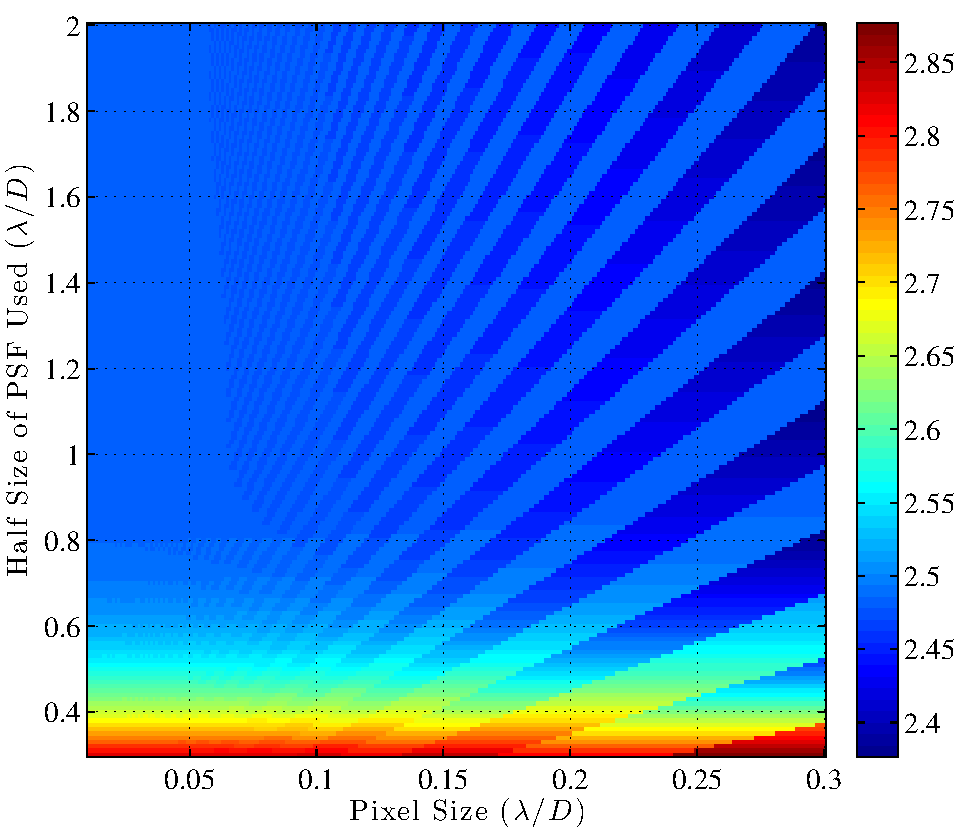
\includegraphics[width=5in]{./figures/intTimevPSF}
  \caption[Integration time vs.~PSF sampling ]{ \label{fig:intTimevPSF} Normalized integration time ($\beta T t$) as a function of half size PSF used and pixel area for an open circular aperture.  The color bar is log-scale, in powers of 10.  Note that insufficient sampling of the PSF can significantly increase the required integration time.}
\end{figure} 

To calculate the value of $Q$ (defined in \refeq{eq:Qdef}) we first define the value:
\begin{equation}
c_1 \triangleq  \textrm{QE} \, \upsilon \Delta\lambda A T t \,.
\end{equation}
This allows us to write:
\begin{equation}\label{eq:Cpdef}
C_p = \mathcal{F}_0 10^{-(V_s + \Delta\textrm{mag})/2.5} c_1 \,,
\end{equation}
and
\begin{equation}\label{eq:Cbdef}
\begin{split}
C_b = &\mathcal{F}_0 10^{-\Omega_{zodi}/2.5} \left(f(\bar{\beta}) +\mu f(I)2.5^{4.78 - M_V} \right) \Delta \alpha c_1\\
&{}+\mathcal{F}_0 10^{-V_s/2.5} C c_1 + \textrm{DR} t + \frac{\sigma_r^2}{t_r}t \,,
\end{split}
\end{equation}
where $C$ is the instrument's designed contrast,  $\Omega_{zodi}$ is the detection band intensity of local zodiacal light in magnitudes per square arcsecond at the ecliptic pole (nominally,  23.34 for V band), $M_V\addsymbol{$M_V$}{Absolute magnitude (V band)}$ is the absolute magnitude of the target star, $\mu\addsymbol{$\mu$}{Brightness of exo-zodi}$ is the brightness of the extrasolar zodiacal light (exo-zodi) in units of local zodi, $\sigma_r$ is the detector read noise, $t_r$ is the exposure time per readout, DR is the detector dark current rate per pixel, and $\Delta\alpha$ is the pixel area on the sky in square arcseconds.  The pixel area can be written as:
\begin{equation}
\Delta \alpha =\Omega\left(\frac{180*3600}{\pi}\right)^2 \,,
\end{equation}
where $\Omega$ is the solid angle of a detector pixel in steradians and equals $(\lambda/2D)^2$ for critically sampled systems with circular apertures \citep{brown2005}.  The function $f$ is the empirically derived variation of zodiacal light with viewing angle given by:
\begin{equation}
f(\theta) = 2.44 - 0.0403 \theta + 0.000269 \theta^2
\end{equation}
with $\theta$ in degrees, in the range [0,90] (the relation is mirrored for $\theta \in (90,180]$).  The function is applied to $\bar{\beta}$ - the absolute value of the ecliptic latitude of the target star, and $I$ - the target star system's inclination\footnote{For mult-planet systems, this refers to the inclination of the ecliptic plane.}(D. Lindler,  Personal Communication, 2008). 

It should be noted that a major assumption being made here is that the exo-zodi is uniform and of constant magnitude in the region being observed.  Recent results indicate that this is not an ideal assumption as exozodiacal dust will clump due to the gravitational effects of any planets and will always have color and brightness variations \citep{kuchner2010collisional}.  If we do select a single value for exo-zodi brightness, then it makes sense to use the historical average for our own solar system.  Based on measurements of seafloor sediment isotope concentrations, the historical distribution of zodical dust in the solar system (over the last 80 Myr) is roughly log normal, with a mean of 1.55 zodi (\reffig{fig:zodi_dist}).  It is predicted that 95\% of solar analogs will have zodiacal dust levels in the range of 0.7 to 3.3 zodi, under the assumption that their asteroid and comet populations are similar to those of our solar system \citep{kuchner2008}.
\begin{figure}[ht]
 \begin{center}
   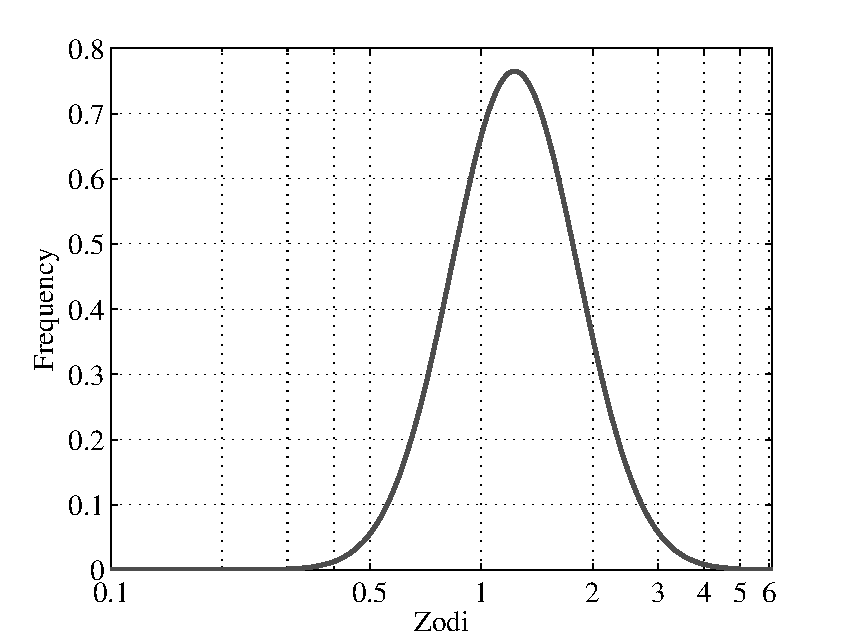
\includegraphics[width=4.5in,clip=true,trim=0.2in 0in 0.5in 0in]{./figures/zodi_dist}
 \end{center}
 \caption[Historical distribution of solar system zodi]{ \label{fig:zodi_dist} Historical distribution of solar system zodiacal dust levels. The distribution is log-normal with geometric mean of 1.55 \citep{kuchner2008}.}
 \end{figure}

Returning to Equations (\ref{eq:Cpdef}) and (\ref{eq:Cbdef}) we evaluate $Q$ as:
\begin{equation}
\begin{split}
Q = \left[\vphantom{\frac{\sigma_r^2}{t_r}} 10^{\Delta\textrm{mag}/2.5} C  + 10^{(V_s +\Delta\textrm{mag}-\Omega_{zodi})/2.5} Z \Delta\alpha \right.
\\
\left. {} + \frac{ 10^{(V_s + \Delta\textrm{mag})/2.5} }{\mathcal{F}_0 \textrm{QE} \, \upsilon \Delta\lambda A T}\left(\textrm{DR} + \frac{\sigma_r^2}{t_r}\right) \right]^{-1} \,,
\end{split}
\end{equation}
 where 
 \begin{equation}
Z = \left(f(\bar{\beta}) +\mu f(I)2.5^{4.78 - M_V} \right)\,.
\end{equation}
In the event of a detection, we calculate the time required for spectral characterization, assuming that the detection integration provides us the magnitude of all background sources.  

Following \citep{lindler2007}, we will represent spectral characterization requirements as minimum signal to noise (S/N$\addsymbol{S/N}{Signal to noise ratio}$) values, using the metric
\begin{equation}
\textrm{S/N} = \frac{C_p}{\sqrt{V}}
\end{equation}
where $V$ is the total variance due to all noise sources.  This value can be written as a function of the square root of the integration time as
\begin{equation}
\textrm{S/N} = \frac{\tilde{C_p} \sqrt{t}}{N_{pix}\left( \left(\frac{\sigma_r^2}{t_r} + \textrm{DR} \right) \left(1 + \frac{1}{N_{dark}}\right) + \mathcal{F}_0 10^{-\Omega_{zodi}/2.5} Z \Delta\alpha \right) + \tilde{C}_p + \tilde{C}_s }
\end{equation}
where $\tilde{C}_p$ and $\tilde{C}_s$ are the planet and star counts per unit time, $N_{dark}$ is the number of dark frames used, and $N_{pix}$ is the number of pixels in the detection box\footnote{This value is often set to the reciprocal of the sharpness (i.e., $N_{pix} = \Psi^{-1}$) \citep{lindler2007}.}.  

The specific S/N value used depends on the spectral feature of interest.  For terrestrial planets, we are especially interested in the possible discovery of biomarkers such as oxygen or ozone.  Several of these features are identified in \citet{heap2007}, along with their S/N requirements; for example, a S/N of 11 for a resolving power of $R = 70$ will produce detections of oxygen at Earth atmospheric levels (21\% ) via the feature at 760nm with a confidence level of over 99.9999\%.  For 20\% Earth O$_2$ abundance, the same signal to noise will still give confidence levels of over 99\% \citep{desmarais2002}.

\section{Astrometry and Doppler Spectroscopy}\label{sec:RV}
While astrometry and doppler spectroscopy employ different technologies and methods to detect planets, they share one thing in common:  namely, these methods infer the presence of planets by tracking the effects of gravitational interactions on the motions of the stars (known as the `astrometric wobble').  The data collected by doppler spectroscopy describes the motion of the target star along the line of sight (the radial velocity), while the data collected by precision astrometry tracks the star's position in the plane of the sky.  Both of these methods therefore require enough observations to fit planetary orbits, which means that the required observing time for confirmed discoveries is directly proportional to the period of planets discovered.  For this reason, there is a strong bias towards short period planets in the early radial velocity data sets \citep{butler2006,cumming2003,cumming2008}.  Similarly, since more massive planets exert a greater effect on their parent stars, these methods are also biased towards larger planets. 

\subsection{Astrometric Observables and Constraints}\label{sec:ast_inst_obs}
\begin{figure}[ht]
\centering
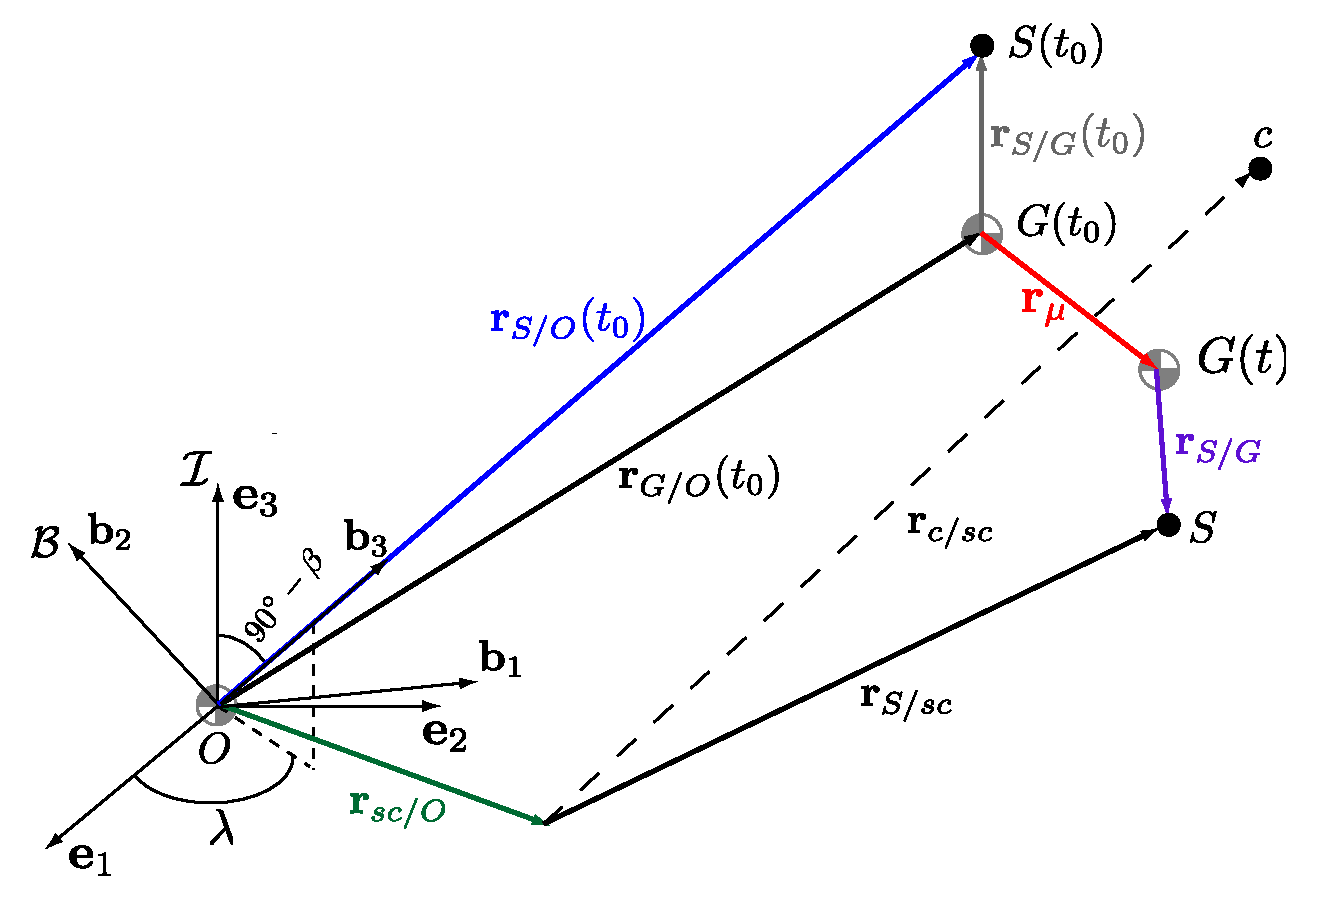
\includegraphics[width=6in]{./figures/ast_model}
 \caption[Astrometric observation schematic]{ A schematic of an astrometric observation.  The solar system barycenter is placed at the origin of frame $\mathcal{I}$, while the observed star system's barycenter at epoch $t_0$ is at $G(t_0)$ and at $G(t)$ at observation time $t$.  $S$ represents the star position at time $t$ and point $c$ represents the (possibly time-varying) position of the centroid of a group of reference stars.}
\label{fig:ast_model} 
\end{figure} 

Figure \ref{fig:ast_model} defines the vectors and reference frames used to describe an astrometric observation of an exosystem.
Reference frame $\mathcal{I}$ is the inertially fixed, barycentric/ ecliptic frame located at the solar system barycenter with the unit vector $\mathbf{e}_3$ directed perpendicular to the ecliptic plane (the $\mathbf{e}_1$ and $\mathbf{e}_2$ unit vectors are arbitrary).  We define a second inertially fixed frame, called the tangent frame, $\mathcal{B}\addsymbol{$\mc B$}{Tangent frame}$, with $\mathbf{b}_3$ axis aligned with $\hat{\R}_{S/O}(t_0)$, the unit vector to the star at the reference time $t_0$.  The $\mathbf{b}_1$ axis is perpendicular to the plane containing $\R_{S/O}(t_0)$ and $\mathbf{e}_3$.  The final unit vector direction, $\mathbf{b}_2$, is mutually perpendicular to $\bc_1$ and $\R_{S/O}(t_0)$.
Given these definitions, we can express the three unit vectors defining $\mathcal{B}$ using coordinates in $\mathcal{I}$ as:
%
\begin{eqnarray}
\hat{\R}_{S/O}(t_0) \equiv \bc_3 &=&  \left[ \begin{array}{ccc} \cos \lambda \cos \beta &\sin \lambda \cos \beta & \sin \beta \end{array}\right]^T_\mathcal{I} \label{eq:rhat_0def} \nonumber\\
\bc_1 &=& \left[ \begin{array}{ccc} 0 & 0 & 1\end{array}\right]^T_\mathcal{I} \times \frac{\hat{\R}_s(t_0)}{\cos\beta} =  \left[ \begin{array}{ccc} -\sin \lambda &\cos \lambda & 0 \end{array}\right]^T_\mathcal{I} \\
\bc_2 &=& \hat{\R}_{S/O}(t_0) \times \bc_1  = \left[ \begin{array}{ccc} -\cos \lambda \sin \beta &-\sin \lambda \sin \beta& \cos \beta \end{array}\right]^T_\mathcal{I} \nonumber
\end{eqnarray}
%
where $\hat\R_{S/O}(t_0)$ is the unit vector to the star as given by its ecliptic coordinates at epoch $t_0$: $(\lambda,\beta)$, measured in the $\mathcal I$ frame.  This definition of frames assumes constant relative velocities between exosystem and local barycenters (i.e., constant proper motions).  For the time scales on which astrometric observations are taken, this is reasonable, but this derivation may have to be expanded if dealing with an accelerating exosystem.

We define the parallax by the small quantity:
\begin{equation}\label{eq:parallaxdef}
\varpi \triangleq \frac{a_0}{\Vert \R_{S/O}(t_0) \Vert} \,,
\end{equation}
where $a_0$ is a distance constant such that $\varpi\addsymbol{$\varpi$}{Parallax}$ is in units of radians.  Thus, $\R_{S/O}(t_0) = (a/\varpi) \hat\R_{S/O}(t_0)$ for $a_0 = 1$ AU, with $\R_s(t_0)$ expressed in AU.  An estimate of $\varpi$ provides the distance to the target star at epoch $t_0$.  The motion of the barycenter of the target star system, $\R_\mu$, is considered as motion in the tangent reference frame,
\begin{equation}\addsymbol{$\R_\mu$}{Exosystem barycenter motion vector}
\R_\mu(t) = \sigma_x (t - t_0) \bc_1 + \sigma_y (t - t_0) \bc_2 + \sigma_z (t - t_0) \hat\R_s(t_0) \,,
\end{equation}
where $\sigma_i$ are the components of barycenter velocity at epoch $t_0$.  We approximate this velocity to be constant, as is usually done when considering short time spans such as  a space-based observatory's lifetime.  This expression is generally split into two components: the transverse and radial velocities.  Following \citet{green1985spherical}, we can write:
\begin{equation}\label{eq:veldef}
\begin{split}
\fddt{I} \R_{G/O}(t) &\equiv  \fddt{I} \left(\R_{G/O}(t_0) + \R_\mu(t)\right) =\fddt{I}\R_\mu(t)\\
  &= V_R  \hat\R_{S/O}(t_0) + \mathbf{V}_T \\
  \textrm{where} \quad  \mathbf{V}_T  &= \hat \R_{S/O}(t_0) \times \left(\fddt{I} \R_{G/O}(t) \times \hat \R_{S/O}(t_0)\right) \, .
 \end{split}
\end{equation}

In our notation, $V_R\addsymbol{$V_R$}{Radial velocity}$ is just $\sigma_z$, whereas $\mathbf{V}_T\addsymbol{$\mathbf{V}_T$}{Transverse velocity}$ is the vector $\left[\begin{matrix} \sigma_x & \sigma_y & 0 \end{matrix}\right]^T$.  The transverse velocity (multiplied by time) thus gives the proper motion of the barycenter (motion in the plane of the sky), which has the largest effect on the position of the target system at the time of observation.  However, the radial velocity also has a measurable effect on the astrometric observation.  Because motion of the target system in the radial direction causes the distance to the system to change, we observe a difference in the direction to the target star, known as `perspective acceleration'.  The third component of $\R_\mu$ (and thus $\sigma_z$) interacts in non-negligible ways with other values in the measurement, and is thus observable.  However, when dealing with \emph{a priori} estimates of these velocity components  it is important to note that the transverse and radial velocities are measured in different ways (i.e., astrometry vs.~doppler spectroscopy).  We will also find it convenient to have an expression for the normalized barycenter motion,
\begin{equation}
\bar{\R}_\mu \triangleq \frac{\R_\mu}{\|\R_{S/O}(t_0)\|} = \bar \sigma_x (t - t_0) \bc_1 + \bar\sigma_y (t - t_0) \bc_2 + \bar\sigma_z (t - t_0) \hat\R_{S/O}(t_0) \,,
\end{equation}
where $\bar\sigma_x$, $\bar\sigma_y$, and $\bar\sigma_z$ are the nondimensional barycenter velocities in radians/time unit.

Finally, we must consider what exactly is measured during an astrometric observation.  While we will focus on astrometric methods that employ interferometers, it is important to note that there are other astrometric instrument designs.  All of these, however, make some measurement of the observer-target star unit vector, and so the analysis above is fully applicable.  An interferometer, in particular, measures the projection of a target direction onto the instrument's baseline vector, recorded as the optical path-length delay (OPD)$\addsymbol{OPD}{Optical path delay}$ between the two interferometer detectors:
\begin{equation}
\textrm{OPD} = \mf B \cdot \hat{\mf r}_{S/sc}  + k + n \,,
\end{equation}
where $\mf B\addsymbol{$\mf B$}{Observatory orientation vector}$ is the orientation vector of an interferometer of baseline length $B = \Vert \mf B \Vert$, $k$ is a constant term representing the offset of the optical path differences, and $n$ is the measurement noise.
Planet-finding is generally proposed in a narrow angle mode, where the measurement is the relative OPD between two sources in a field of view, performed in quick succession such that $k$ remains nearly constant, and is assumed to cancel in subtraction.  Typically each target star has multiple reference sources, so the combined differential OPD ($\Delta$OPD) is with respect to a centroid position.  The measurement is also repeated for two (preferably orthogonal) interferometer baseline orientations to track the 2D position of the target in the plane of the sky.  Assuming that the interferometer baselines are taken as directions $\mf b_1$ and $\mf b_2$ of our body frame, then the astrometric measurement becomes:
\begin{equation}\label{eq:measurement}
\mf d = B\left[ \begin{array}{l} \mf b_1 \cdot \left(\hat{\mf r}_{S/sc} - \hat{\mf r}_{c/sc}\right) \\\mf b_2 \cdot \left(\hat{\mf r}_{S/sc} - \hat{\mf r}_{c/sc}\right) \end{array}\right] + \mf n \,,
\end{equation}
where $B$ is the size of the interferometer baseline and $\mf n$ is an additive noise vector due to measurement error.  

In the literature, the measurement in \refeq{eq:measurement} is often described as the angular separation between the two sources, projected onto the baseline \citep{konacki2002frequency,sozzetti2002,sozzetti2003}; it is assumed that $\mf d$ scaled by $B$ is a radian measure that can be converted to other angular units such as arcseconds.  It is this assumption that leads to the terminology of $\mu$as-precise astrometry, as the required sensitivity of the instrument to changes in the OPDs, when treated as an angle, evaluates to under 1 $\mu$as.  

In fact, \citet{colavita1994measurement} points out that, using the definition for $\hat{\mf r}_{S/sc}$ in \refeq{eq:rhat_0def}, for a centroid separation of ($\Delta \lambda$, $\Delta \beta$), the difference in unit vectors, to first order, can be written as,
\begin{equation}\label{eq:sdiff_fo}
\hat{\mf r}_{S/sc} - \hat{\mf r}_{c/sc} \approx \left[\begin{matrix} 
\sin\beta\cos\lambda\Delta\beta + \cos\beta\sin\lambda\Delta\lambda\\
\sin\beta\sin\lambda\Delta\beta - \cos\beta\cos\lambda\Delta\lambda\\
-\cos\beta\Delta\beta \end{matrix}\right]_\mathcal{I} \, .
\end{equation}
In this way, knowledge of the baseline vector and the differential OPD allows you to calculate a vector which maps in a relatively simple fashion (to first order) to two spherical angles representing the separation between the target and centroid.

\begin{figure}[ht]
\centering
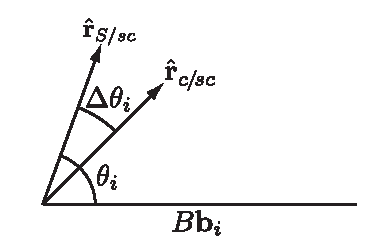
\includegraphics[width=2.75in]{./figures/narrow_angle_model}
 \caption[Narrow angle astrometry schematic]{ A schematic of a narrow-angle astrometric measurement.  $B$ is the size of the interferometer baseline.}
\label{fig:narrow_mode_model} 
\end{figure} 

Unfortunately, such a direct first order mapping between \refeq{eq:measurement} and the angle between the target and centroid is not very accurate.  An OPD has units of distance or time (with the converting factor equal to the speed of light), and so a differential OPD will also have values equal to fractions of the interferometer baseline.  Let us assume that the (flat) wavefront from the target star is incident on the interferometer baseline with angle $\theta_i$, and that the centroid is located at an angle $\Delta\theta_i$ from the target star, in the projection of the sky due to interferometer orientation $\mf b_i$ (Figure \ref{fig:narrow_mode_model} --- $\Delta\theta_i$ is analogous to $\Delta\lambda$ and $\Delta\beta$ in \refeq{eq:sdiff_fo}).
The components of the measurement (without the noise term) are then,
\begin{equation}
d_i =B \left(\cos\theta_i - \cos(\theta_i - \Delta\theta_i)\right) =B\left(\cos\theta_i(1 - \cos\Delta\theta_i) - \sin\theta_i \sin\Delta\theta_i\right) \,.
\end{equation}

We are primarily interested in changes in the angle $\Delta\theta_i$, since this determines the movement of the target star with respect to the centroid in time (of course, this is further complicated by possible motion of the centroid itself).  Assuming this to be a small angle, we can substitute the Taylor series expansions of the sine and cosine terms in $\Delta\theta_i$ to first order to find,
\begin{equation}
d_i \approx -B \sin\theta_i \Delta\theta_i \, .
\end{equation}
Thus, by scaling the differential OPD by the interferometer baseline length and the direction on the sky of the target ($B\sin\theta_i$), we do get a first order approximation of the angular difference between the target and centroid (assuming perfect a priori knowledge of the target's (or equivalently centroid's) location with respect to the interferometer orientation).  Unfortunately, if we assume the target star to be on the order of 1$^\circ$ from the centroid \citep{sozzetti2002,shao1992potential}, the first of the dropped terms ($\Delta\theta_i^2/2$) has a magnitude of 1.5$\times10^{-4}$ rad, or 31.4 arcseconds.  When discussing ultra-precise applications, it is therefore inaccurate to treat the values produced by \refeq{eq:measurement} as directly mapping to angular measures.  For these reasons, we treat all derived values as dimensionless for the remainder of this discussion, normalizing all distances and converting all angles to radians to remain consistent.  It is also important to point out that in this discussion, we consistently assume zero pointing error.  For a real instrument, accurate knowledge of the baseline vectors will be built up over many individual observations, each with an associated measurement error, but neither the interferometer orientation, nor the exact length of the baseline, can ever be known with perfect precision.  In order to include a pointing and baseline length error, we would need to extend the measurement equation, and update all subsequent calculations.

With these definitions and considerations, we can write the exact astrometric measurement  in terms of known quantities and the quantities whose values we wish to determine.  This is done by writing the vector from the spacecraft to the target star, $\mf r_{S/sc}$, in terms of the initial reference vector, $\R_{S/O}(t_0)$,
%
\begin{eqnarray}
\R_{S/sc} & = & \R_{S/O}(t_0) - \R_{S/G}(t_0) + \R_\mu + \R_{S/G} - \R_{sc/O} \nonumber \\
& = & \R_{S/O}(t_0) + \R_\mu + \Delta \R_{S/G} - \R_{sc/O} \,,
\end{eqnarray}
where $\R_{sc/O}$ is the spacecraft position vector relative to the solar system barycenter and  $\Delta \R_{S/G}$ is the difference in the star's position relative to $G$ between $t_0$ and epoch. We can then find the unit vector in the direction of $\R_{S/sc}$,
%
\begin{equation}\label{eq:rhat_ssc}
\begin{split}
\hat\R_{S/sc} &= \frac{\R_{S/sc}}{\| \R_{S/sc} \|}  \\
&= (\R_{S/O}(t_0) + \R_\mu +\Delta \R_{S/G}- \R_{sc/O})\times  \\
&\hspace{3ex}  \left\{\R_{S/O}(t_0)\cdot\R_{S/O}(t_0) + \R_\mu \cdot \R_\mu + \Delta \R_{S/G} \cdot \Delta \R_{S/G} +\R_{sc/O} \cdot \R_{sc} \right. \\
&\hspace{3.5ex}{}+ 2\R_{S/O}(t_0) \cdot \R_\mu + 2\R_{S/O}(t_0) \cdot \Delta \R_{S/G} - 2\R_{S/O}(t_0) \cdot \R_{sc/O} \\
&\hspace{3.5ex}\left.{} + 2 \R_\mu \cdot \Delta \R_{S/G} - 2 \R_\mu \cdot \R_{sc/O} - 2 \Delta \R_{S/G} \cdot \R_{sc/O}\right\}^{-\frac{1}{2}} \,. 
 \end{split}
\end{equation}

The spacecraft to centroid pointing unit vector, $\hat{\mf r}_{c/sc}$, can be similarly expressed by using \refeq{eq:rhat_ssc} for each reference source with the appropriate values for $\R_{S/O}(t_0)$ and $\R_\mu$.  When using this model for the reference sources, it is important to note that for a source $n$, $\hat\R_{n}(t_0)$ is not aligned with $\hat\R_{S/O}(t_0)$ and is thus not orthogonal to $\mf b_1$ and $\mf b_2$.  When evaluating \refeq{eq:measurement}, this simply means that all vectors have to be expressed as components in the same reference frame, which requires a change of coordinates for the reference sources.  If we assume extragalactic references with no companions or planets, the variation in the centroid position will be many orders of magnitudes below our desired level of accuracy.  Unfortunately, such references are not always available, and so these effects may become significant if one or more of the references is within our galaxy and has companions of its own.

\subsection{Doppler Spectroscopy Observables and Constraints}\label{sec:rv_inst_obs}
Unlike astrometry, which uses interferometers to find the instantaneous position of the star in the plane of the sky, doppler spectroscopy utilizes high-resolution spectrometers to measure the instantaneous velocity of the star along the line of sight.  Calibration sources such as cathode lamps and absorption cells are used to produce highly accurate spectra \citep{vogt1994hires}.  Following \citet{marcy1992precision} and \citet{butler1996attaining}, we model the observation as starlight passing through an absorption cell (e.g., iodine), which creates a combined spectrum of absorption bands from the star's spectrum and the cell.  This combined spectrum is passed through an echelle spectrometer \citep{vogt1987lick} and dispersed onto the detector as a nearly linear function in wavelength.

Any shift in the stellar spectrum must be modeled as due to Doppler effects and instrumental effects including mechanical instabilities, thermal effects, and the alignment of the optical system.  The observed spectrum can then be written as:
\begin{equation}\label{eq:obsSpectrum}
I_{obs}(\lambda) = \kappa \left[ I_S(\lambda + \Delta\lambda_S)T_C(\lambda + \Delta\lambda_C) \right] \otimes \PSF
\end{equation}
where $I_S$ is the stellar spectrum, $\Delta\lambda_S$ is the shift of the stellar spectrum, $T_C$ is the transmission function of the absorption cell, and $\Delta\lambda_C$ is the shift of the transmission function. The constant $\kappa$ is directly proportional to the integration time of the observation.  The transmission function is measured directly with the use of another spectrometer (for example a Fourier Transform Spectrometer \citep{davis2001fourier}), while the stellar spectrum may be derived from high signal-to-noise observations of the target star by means of PSF deconvolution \citep{gilliland1992resolution}.  The remaining parameters are determined by fitting the observed spectrum to \refeq{eq:obsSpectrum}.

The Doppler shift is parameterized as $\Delta\lambda/\lambda$, where:
\begin{equation}
\Delta\lambda \triangleq \Delta\lambda_S - \Delta\lambda_C \,.
\end{equation}
This can be related to the star's velocity via the relativistic Doppler equation:
\begin{equation}\label{eq:doppler}
\frac{\Delta\lambda}{\lambda} = \frac{\left(1 + \left(\frac{v}{c}\right)^2\cos\theta\right)\left(1 + \rho_g\right)}{n\sqrt{1 - \left(\frac{v}{c}\right)^2}} - 1
\end{equation}
where $n$ is the index of refraction of the air column over the spectrograph and  $\rho_g$ is the gravitational redshift of the starlight.  The velocity $v$ is defined as the magnitude of the velocity of the target star with respect to the observer ($v = \Vert \leftexp{\mc I}{\mf v_{S/sc}}\Vert$) while $\theta$ is the angle between the line of sight and the star's velocity vector:
\begin{equation}
\cos\theta = \hat{\mf r}_{S/sc}\cdot \leftexp{\mc I}{\hat{\mf v}_{S/sc}} \,.
\end{equation}

If we take $\theta = 0$ \refeq{eq:doppler} becomes:
\begin{equation}
\frac{\Delta\lambda}{\lambda} = \frac{\left(1 + \rho_g\right)}{n} \sqrt{\frac{\left(1 + \frac{v}{c}\right)}{1 -\frac{v}{c}}} - 1 \,.
\end{equation}
If $v \ll c$, the Taylor expansion of this expression gives us:
\begin{equation}
\frac{\Delta\lambda}{\lambda} = \frac{\left(1 + \rho_g\right)}{n}\left(1 + \frac{v}{c} + \mc O\left( \left(\frac{v}{c}\right)^2\right) - 1\right) \approx \frac{v}{c} \,.
\end{equation}
We thus have an approximate linear mapping of the doppler spectroscopy observables to the star's line of sight velocity.  Current ground-based observations have precisions of order 1 m s$^{-1}$ \citep{butler2006}, although improvements in instrumentation and calibration may provide us with precisions of order 1 cm s$^{-1}$ in the near future \citep{lovis2006exoplanet}.  Together with the astrometric measurement, doppler spectroscopy provides a third spatial component, making the full three-dimensional orbit observable, given that sufficient measurement accuracy is achieved.


\section{Transit Photometry}\label{sec:photometry}

Of all of the methods so far discussed, transit photometry has the largest resource requirements as it demands constant monitoring of the target star.  It also represents the least likely event, since the orientation of the orbit has to be such that the planet will obscure the star at some point, from the point of view of the observer.

\begin{figure}[ht]
\centering
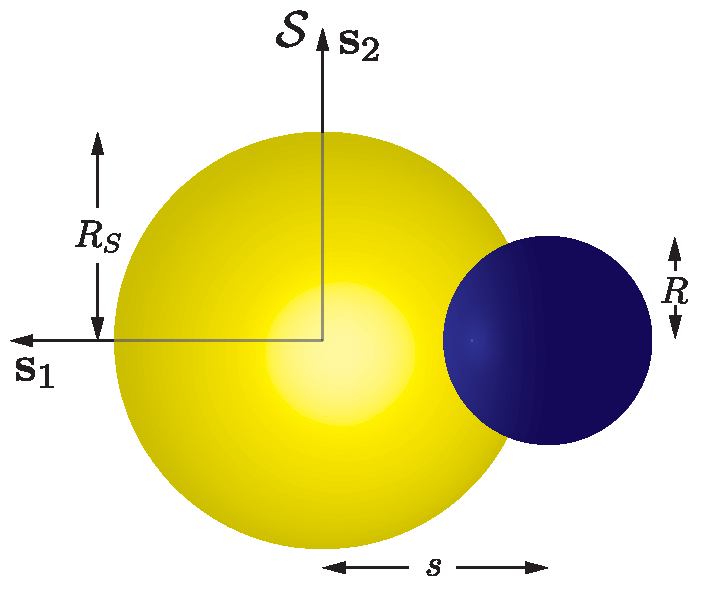
\includegraphics[width=4in]{./figures/phot_model}
 \caption[Transit schematic]{ A schematic of a photometric transit observation.  The amount of starlight occluded from the observer's point of view is determined by the star and planet radii ($R_S$ and $R$) and the apparent separation $s$.}
\label{fig:phot_model} 
\end{figure} 

\reffig{fig:phot_model} presents a schematic view of a transit in the plane of the sky.  The amount of starlight occluded can be expressed as a function of the star and planet radii and the apparent separation.  Following \citet{mandel2002analytic}, we can express the ratio of obscured ($F^{(e)}_S\addsymbol{$F^{(e)}_S$}{Obscured stellar flux}$) to unobscured starlight, assuming a uniform source and an opaque eclipsing body, as:

\begin{equation} \label{eq:transitFe}
 \frac{F^{(e)}_S}{F_S} = 
\left\{ \begin{array}{l l}
1 & R_S + R < s\\
1 - \frac{1}{\pi} \left[ \frac{R^2 }{R_S^2}\kappa_0 + \kappa_1 - \sqrt{\frac{s^2}{R_S^2} - \frac{\left( R_S^2 + s^2 - R^2\right)^2}{4 R_S^4}}\right] & \vert R_S - R \vert < s \le R_S + R \\
1 - \left(\frac{R}{R_S}\right)^2 & s \le R_S - R\\
0 & s \le R - R_S
\end{array} \right. 
\end{equation}
where
\begin{equation}
\kappa_0 = \cos^{-1}\left(\frac{R^2 +s^2 - R_S^2}{2Rs}\right) \quad\textrm{and}\quad \kappa_1 =  \cos^{-1}\left(\frac{R_S^2 - R^2 + s^2}{2R_S s}\right)
\end{equation}
where $R_S\addsymbol{$R_S$}{Star radius}$ is the stellar radius.

These equations allow us to model the `dip' in the photometric output of an exosystem associated with a transiting exoplanet, but there are many additional photometric effects that can be observed.  Stars are not perfectly uniform sources, which produces limb darkening and  causes more significant dimming during eclipse \citep{mandel2002analytic,claret2008testing}.  Furthermore, effects due to atmospheric lensing and projected oblateness can be inferred from sufficiently precise transit photometry \citep{hui2002atmospheric}.  While all of these can improve our modeling of exosystems, they will not be explicitly considered in this thesis.  However, as these effects may be modeled using the same parameter set employed throughout this chapter, they may be simulated and analyzed using the same methods that will be introduced in Chapters \ref{ch:param_dists} and \ref{ch:obs_sims}.

 % Obs Methods
\chapter{Parameter Distributions and Detection Probabilities}\label{ch:param_dists}

\section{Current State of Knowledge}\label{sec:curr_param_dists}
The distributions of the physical and orbital parameters of exoplanets change rapidly as the pace of exoplanet discovery accelerates.  As of this writing, this entire population is being transformed as the Kepler mission continuously introduces new candidates potentially doubling the total number of known exoplanets \citep{borucki2010kepler}.  Multiple groups are maintaining and updating catalogues of exoplanets and are actively working on deriving the distributions of planetary and orbital parameters \citep{marcy2005observed,cumming2008,mordasini2009extrasolarI,mordasini2009extrasolarII}.  One of the most important results of this work is the identification of a power-law trend in the relationship between projected mass ($m_P \sin I$) and period in radial velocity survey data.  \reffig{fig:cummingData} shows data from the Keck planet search, while \reffig{fig:cummingMPfit} shows the resulting power-law fit to the model:
\begin{equation}\label{eq:powerlawModel}
\intd{N}  =  c m_P^\alpha P_{orb}^\beta \intd{\log m_P}  \intd{\log P_{orb}} \,,
\end{equation}
where $c$ is a constant of proportionality.  This work is very useful in generating sample planetary systems as in \S\ref{sec:gen_plan_sys}.

\begin{figure}[ht!]
\centering
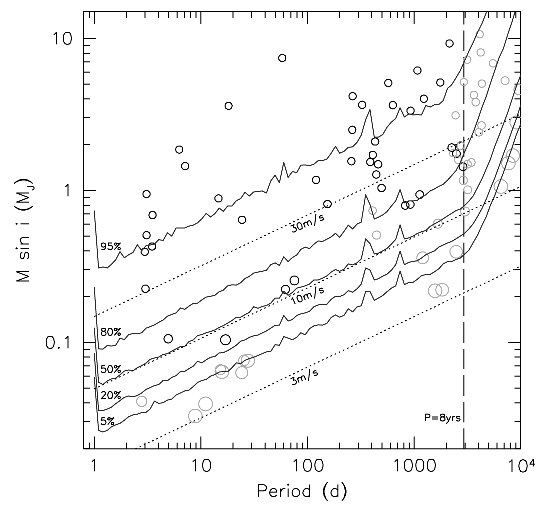
\includegraphics[width=5.5in]{./figures/cummingData}
 \caption[$m_P\sin I - P_{orb}$ Data]{ Detections for F, G, and K stars corrected for completeness of the survey. Black circles are confirmed planets circa May 2005 and gray circles are candidates with circle size indicating the magnitude of selection effects for each. The vertical dashed line indicates a period of 8 years and the dotted lines show velocity amplitudes of 3, 10, and 30 m/s for a 1 M$_\odot$ star. For a given period, the solid curves show the mass that can be ruled out at the 99\% level from 5\%, 20\%, 50\%, 80\%, and 95\% of stars. From \citet{cumming2008}.}
\label{fig:cummingData} 
\end{figure} 

\begin{figure}[ht]
\centering
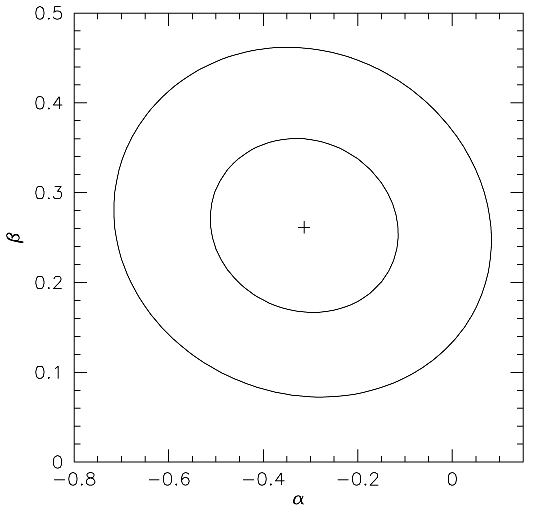
\includegraphics[width=4.5in]{./figures/cummingMPfit}
 \caption[$m_P\sin I - P_{orb}$ power-law fits]{ Contours of constant likelihood for a fit to \refeq{eq:powerlawModel} . The contours correspond to the 68\% and 95\% confidence intervals with best-fit values of  $\alpha = -0.31$ and $\beta = 0.26$.  From \citet{cumming2008}.}
\label{fig:cummingMPfit} 
\end{figure} 

Similarly, much work has been done to constrain the density distributions of known planets, relating planetary masses and radii.  As shown in \citet{fortney2007}, the densities of rocky planets can be modeled to a high degree of accuracy by assuming that the planets are composed of either a rock/ice or a rock/iron mixture.  These assumptions lead to the relations:
\begin{equation}\label{eq:rockyPlanDensities}
R = \left\{ \begin{array}{l l} 
\begin{array}{l} (0.0912(1-\textrm{rmf}) + 0.1603)(\log m_P)^2\\ + (0.3330(1-\textrm{rmf}) + 0.7387)\log m_P \\
{} + (0.4639 (1-\textrm{rmf}) + 1.1193) \end{array} & \textrm{ice/rock} \\\\
\begin{array}{l} (0.0592\textrm{rmf} + 0.0975)(\log m_P)^2\\ + (0.2337\textrm{rmf} + 0.4938)\log m_P \\
{} + (0.3102\textrm{rmf} + 0.7932) \end{array} & \textrm{rock/iron}
\end{array} \right.
\end{equation}
where the planetary radius is measured in $R_\oplus$, the planetary mass in $M_\oplus$ and rmf is the fraction of rock.  The resulting density curves are shown in \reffig{fig:fortneyDensities}.  For giant planets, radii values may be interpolated from a lookup table based on known values by assuming the fraction of the planet's mass contained in the core \citep{fortney2007}.  Density modeling is especially important in simulating direct imaging as both the planet radius and planet mass must be defined to generate the observable quantities and to propagate the planet on its orbit.

\begin{figure}[ht]
\centering
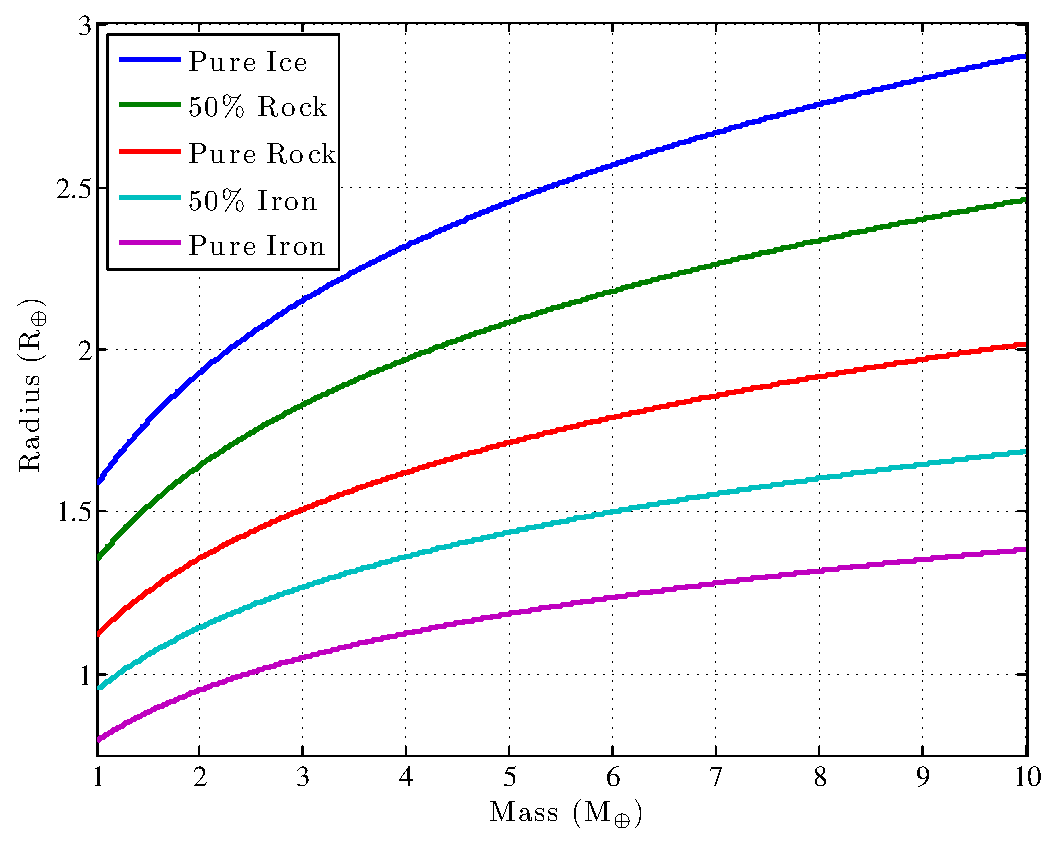
\includegraphics[width=5.5in]{./figures/fortneyDensities}
 \caption[Rocky planet densities]{ Densities of rocky planets modeled as rock/ice and rock/iron mixtures \citep{fortney2007}.}
\label{fig:fortneyDensities} 
\end{figure} 

Another important observed correlation is between the occurrence of exoplanets and the metallicity of the host star.  Surveying a population of  FGK stars, \citet{marcy2005observed} found planets around approximately 25\% of the most metal-rich stars (i.e.,  [Fe/H] > 0.3) and around only 3\% of metal poor stars ([Fe/H] < -0.5).  The occurence of planets as a function of [Fe/H] can also be fit to a power-law---gas giant detections are nearly proportional to the square of the number of iron atoms of the host star, with constant of proportionality of about 0.03 (\reffig{fig:marcyFEH}).  This may be an important factor in the selection of a target list, especially as a final filter to pinpoint the highest detection probability targets (see \S\ref{sec:targ_selection}).

\begin{figure}[ht]
\centering
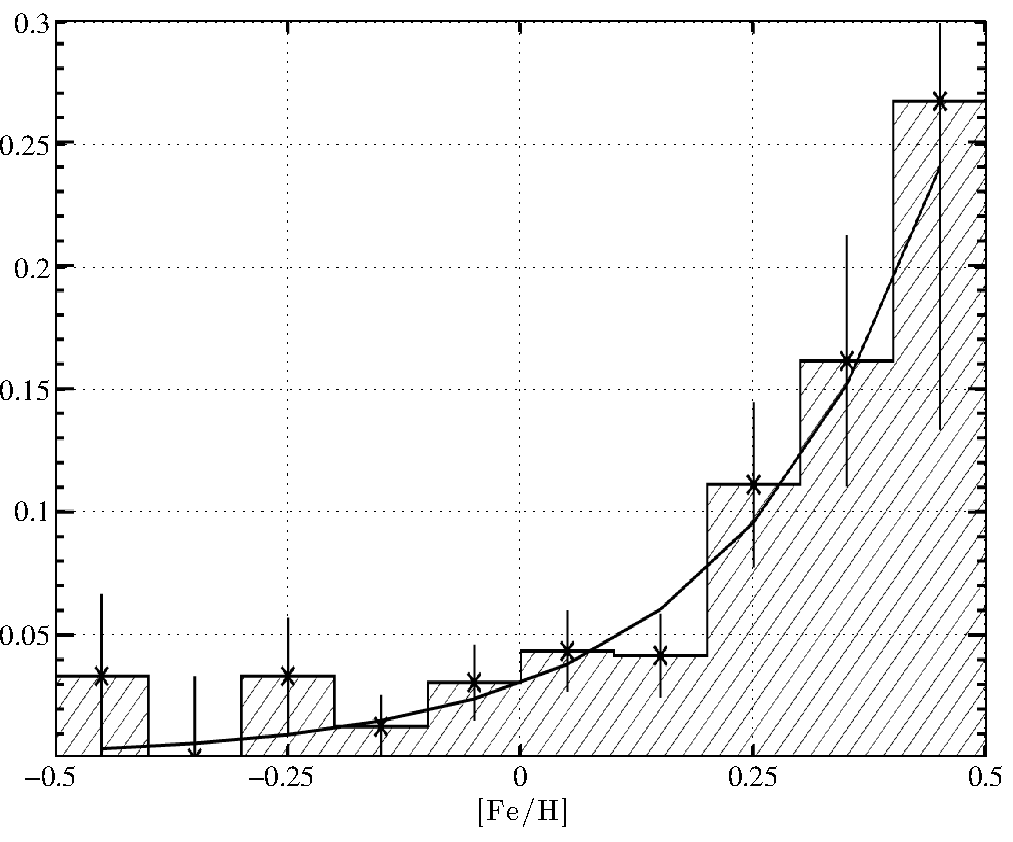
\includegraphics[width=5.5in]{./figures/marcyFEH}
 \caption[Planet occurence vs metallicity]{ Portion of host stars with planets as function of iron abundance [Fe/H] star. Data from \citet{marcy2005observed}.}
\label{fig:marcyFEH} 
\end{figure} 


\subsection{Biases}\label{sec:biases}
If we plot a snapshot of the available orbital parameters for the currently known exoplanets, as in \reffig{fig:currHists}, we immediately notice several prominent, and potentially misleading, features.  There appears to be a large bias towards low eccentricity and semi-major axis.   The low semi-major axes preference is due to the inherent bias in detection methods that require full (or even multiple) periods of data before a detection can be validated.  These methods inherently detect more short period planets and as they include astrometry, radial velocity and transit photometry, which were used to find the majority of known exoplanets, the data set contains a disproportionately large number of short period (and thus low semi-major axis) planets.  The low eccentricity accumulation is due to a specific population of planets: tidally locked short period gas giants  or `hot Jupiters'.  These are easily detected due to their large size and short period, and all have near zero eccentricity due to orbital circularization.

\begin{figure}[ht]
\centering
\subfigure[Mass]{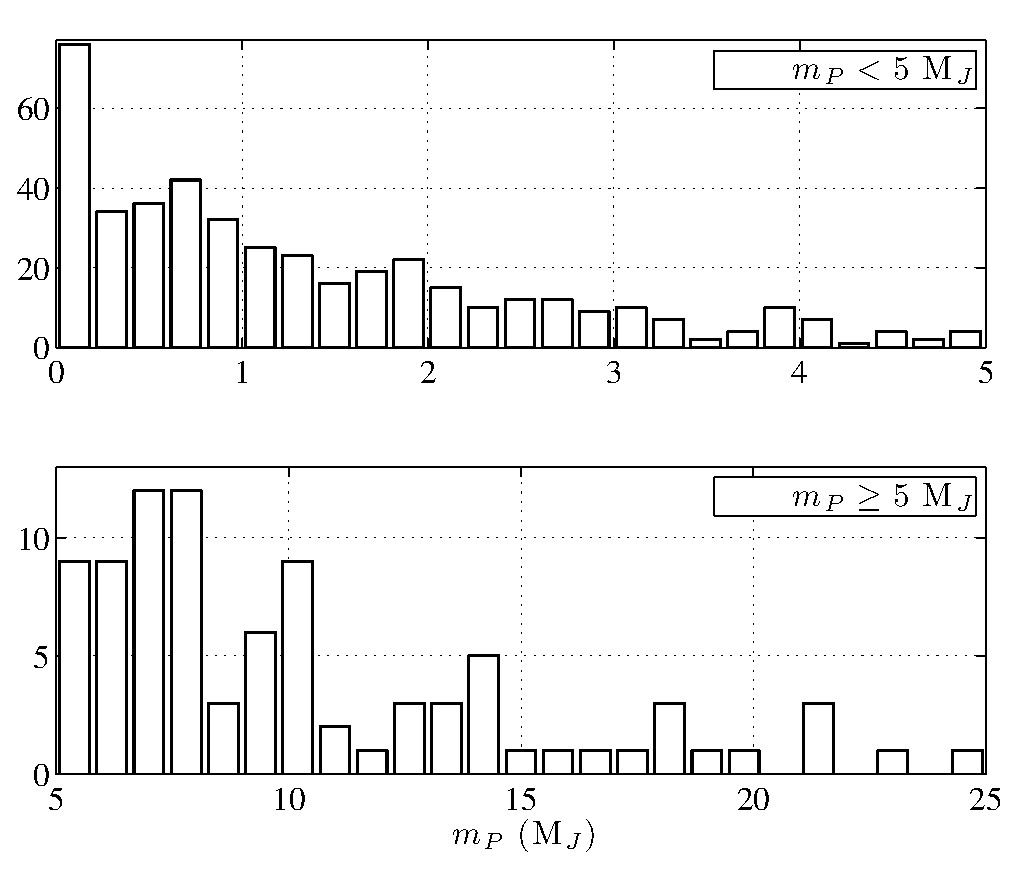
\includegraphics[width=2.9in]{./figures/currMassHist}\label{fig:currMassHist}}
\subfigure[Semi-major axis]{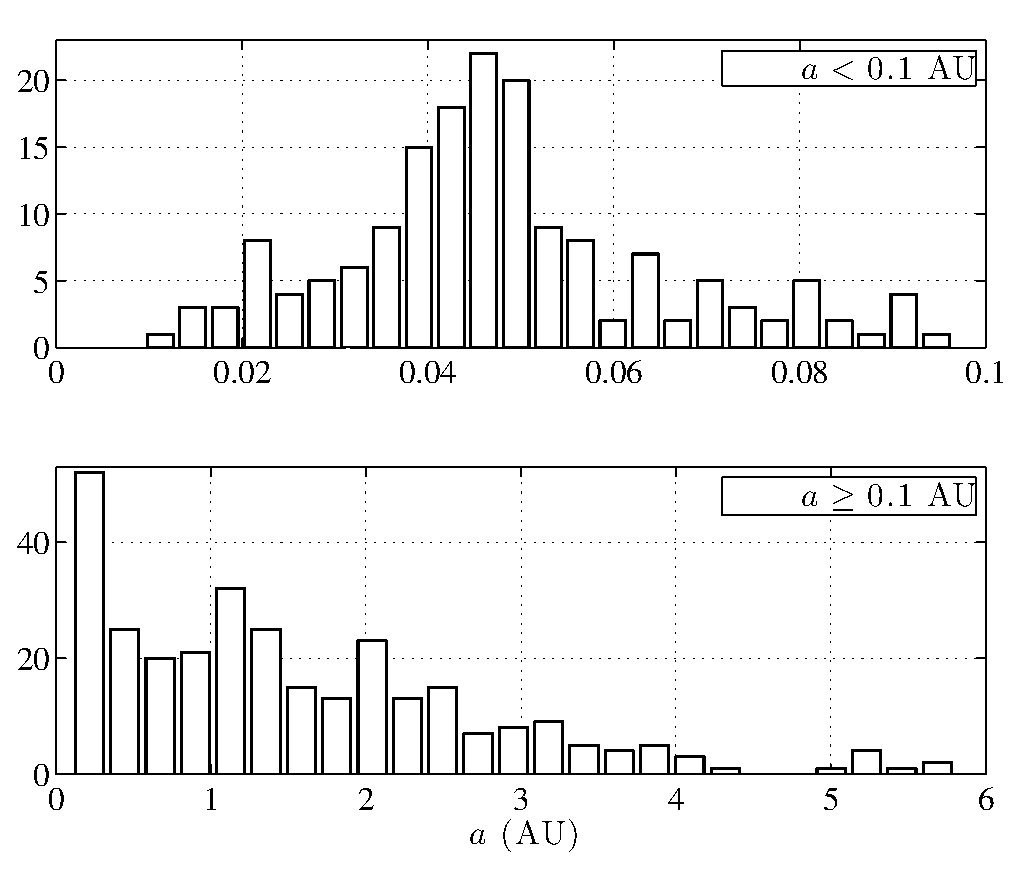
\includegraphics[width=2.9in]{./figures/currSMaxHist}\label{fig:currSMaxHist}}
\subfigure[Eccentricity]{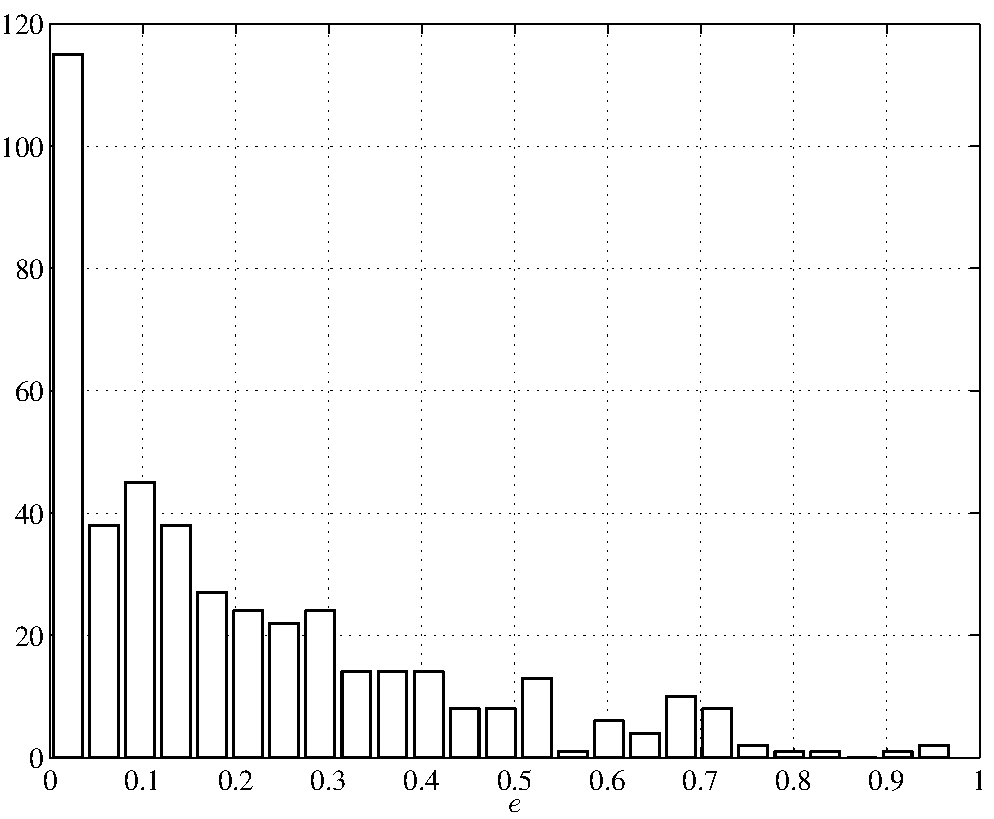
\includegraphics[width=3.5in]{./figures/currEccenHist}\label{fig:currEccenHist}}
 \caption[Orbital parameter distributions of currently known exoplanets]{Histograms of orbital parameters of currently known exoplanets. Retrieved from the NASA/IPAC/NExScI Star and Exoplanet Database \url{http://nsted.ipac.caltech.edu} on April 17th, 2011. \label{fig:currHists}}
\end{figure}  

Much work has been devoted to trying to find the true distributions of these parameters using both detailed modeling \citep{currie2009semimajor} and data analysis \citep{hogg2010inferring}.  These efforts all seek to incorporate not just the raw data, but also the instrumental biases and the likelihoods of the individual detections.  Another important point is to consider inherent biases in the parameters themselves---for example, as eccentricity is defined within a strictly bounded range, it tends to be overestimated, introducing another source of bias.  In the remainder of this chapter, we will consider how to model the likelihood of planetary detections, as well as the Keplerian elements used for describing planetary orbits.

\section{Observational Completeness}\label{sec:completeness}
\citet{brown2004a} introduced the concept of completeness to study the selection effects introduced by observatory architectures on direct detection searches for sub-stellar companions.  Assuming distributions for the semi-major axis and eccentricity of planetary orbits, Brown calculated the probability that a companion's angular separation would fall outside the telescope's IWA during an observation of its parent star.  \citet{brown2005} subsequently expanded this concept to include the selection effects due to the telescope specific photometric restrictions on observability (i.e., $\Delta$mag$_0$), and \citet{brown2009} demonstrated how completeness could be evaluated for indirect companion detection methods such as astrometry.  Completeness has also been extended to account for multiple observations of one star at different times \citep{brown2010new}, and has been utilized in mission analysis and development for a variety of proposed exoplanet observatories \citep{savransky2010,brown2009} as will be detailed in \refch{ch:obs_sims}.

The direct detection completeness is evaluated by assuming that a companion will be observable if its angular separation from the star is greater than the observatory's IWA, and illuminated such that the difference in brightness between star and companion is below the limiting $\Delta$mag.  To calculate the completeness, probability distributions (or constant values) are assumed for planetary orbital elements and physical properties.  A large, equal number of samples is generated from each distribution, and the star-planet angular separation and $\Delta$mag are calculated for each set of samples.  When binned in a two-dimensional histogram, these generate a density function representing the probability that a planet drawn at random from the assumed population will have a given angular separation and $\Delta$mag (\reffig{fig:earthTwin_pdf}).  Integrating over this density yields a cumulative distribution function (CDF).  An instrument with a given $\Delta$mag$_0$ and IWA, observing a star with a planet from the assumed population, has a probability of detecting the planet upon its first observation equal to the corresponding CDF point \reffig{fig:earthTwin_cdf}).

\begin{figure}[ht]
\centering
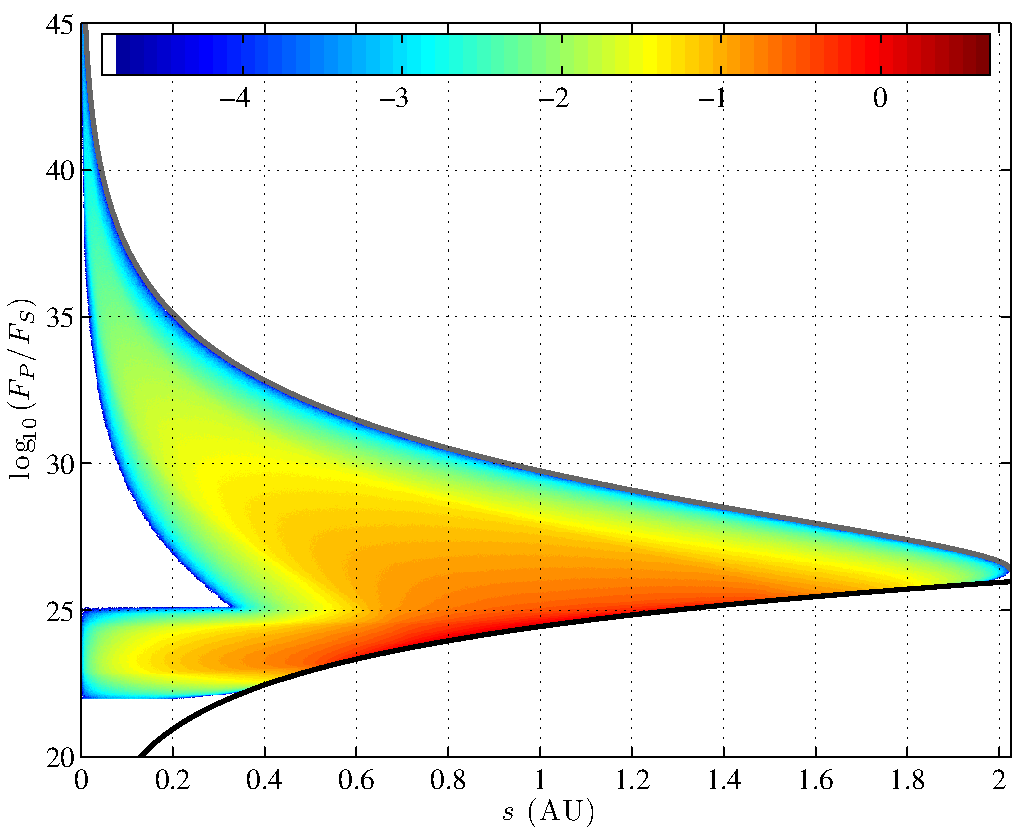
\includegraphics[width=5.5in]{./figures/earthTwin_pdf}
 \caption[Earth-twin observation PDF]{ Observational and photometric completeness for a population of Earth-twin planets ($a \in [0.7, 1.5]$, $e \in [0, 0.35]$, $p = p_\oplus$, $R = R_\oplus$).  The joint probability density function of ($\bar s = s,\bar F_P/F_S = F_P/F_S$) is sampled via 1 billion Monte Carlo trials, and the 2D histogram is constructed by counting the number of occurrences in each grid square scaled by total number of samples and the grid square area. The colorbar is log-scale, in powers of 10 and the bounding solid lines (black and gray) are calculated via Equations (\ref{eq:maxFr}) and (\ref{eq:minFr}).  The black line does not bound the histogram for all values of $s$ because of the limits on $a$ placed on the input distribution.}
\label{fig:earthTwin_pdf} 
\end{figure} 

\begin{figure}[ht]
\centering
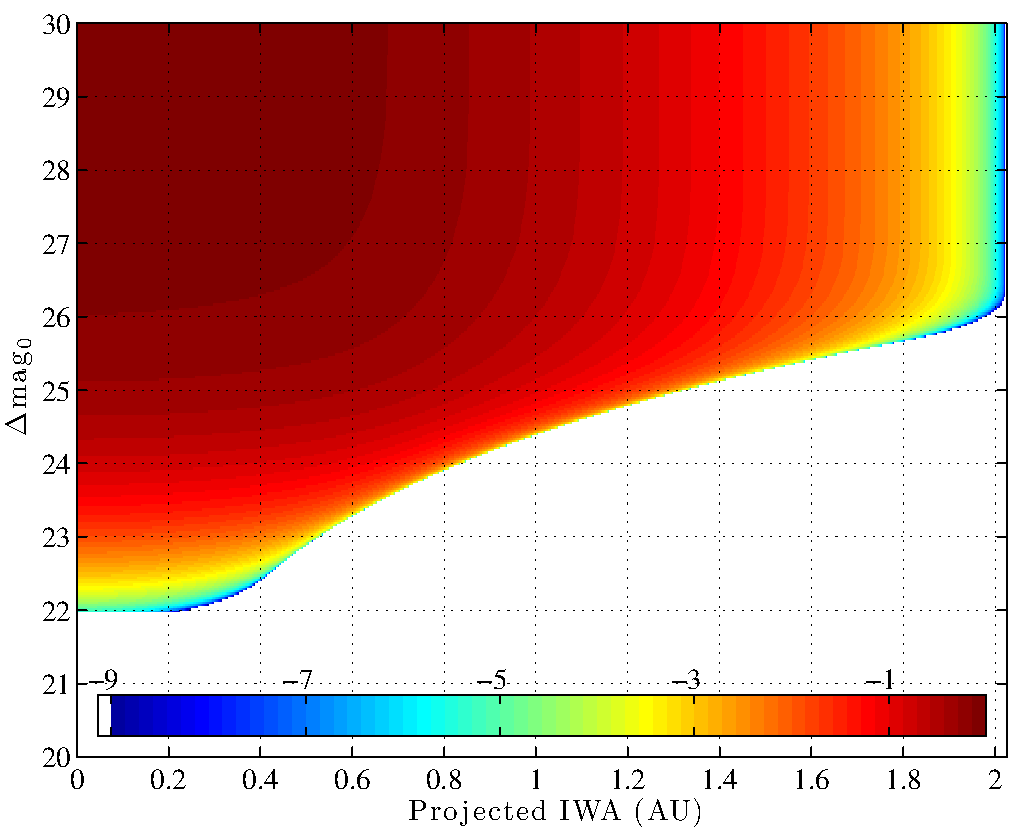
\includegraphics[width=5.5in]{./figures/earthTwin_cdf}
 \caption[Earth-twin observation CDF]{Integrated observational and photometric completeness from \reffig{fig:earthTwin_pdf}. The colorbar is log-scale, in powers of 10, representing the cumulative distribution function of the random variable in \reffig{fig:earthTwin_pdf}.  The CDF is calculated by summing across the rows and columns of the (unscaled) PDF histogram at each grid square and scaling the result by the total number of samples.  The histogram is truncated at $\Delta$mag$_0$ of 30, as the CDF becomes nearly constant for a given projected IWA for $\Delta$mag$_0 > 27$, as demonstrated by the vertical bands of nearly constant color.  The CDF is unity at zero projected IWA and $\Delta$mag$_0 > 53$.}
\label{fig:earthTwin_cdf} 
\end{figure} 

\subsection{Applications}\label{sec:completeness_apps}
This definition of completeness describes the conditional detection probability (given the instrument capabilities and that a planet exists in the target system) only for the first target system observation.  Subsequent observations of the same exosystem do not represent independent samples, and will thus have different detection probabilities.  If each observation was fully independent of the others, with constant detection probability ($p_c$) equal to the single visit completeness, then the probability of $k$ successful detections in $n$ visits would be  given simply by the binomial theorem as:
\begin{equation}
P_n(k) = \binom{n}{k} p_c^k (1-p_c)^{n-k} \, .
\end{equation}
The probability of any (non-zero) number of detections in $n$ visits would then be
\begin{equation} \label{eq:multvisit_detprob}
P_n(k>0) = 1 -  \binom{n}{0}  p_c^0 (1-p_c)^{n} = 1 - (1-p_c)^n\, .
\end{equation}
In reality the probability of detecting a planet on subsequent visits is conditionally dependent on the planet's orbit and the times between observations, but this equation gives a good upper bound for the probability of detecting a planet (given that one exists) over multiple visits.  

We can demonstrate this bound empirically by running Monte Carlo simulations of 1 million orbits in the habitable zone of a given star and tracking the aggregate number of detections over multiple visits.  The results are shown in \reffig{fig:compSim}.  All of the planets are modeled as Earth-twins, and the instrument is assumed to have a limiting $\Delta$mag of 26.  The star's luminosity and distance and instrument's IWA  are chosen so that the projected IWA corresponds to the inner edge of the habitable zone (i.e., the projected IWA is at 0.70 AU for a star of 1 L$_\odot$).  The single visit completeness of this star for Earth-twins on habitable-zone orbits is approximately 0.5162.  The plots show the results of returning every 1, 2, and 4 weeks, as well as daily revisits, randomly timed revisits, and the values of \refeq{eq:multvisit_detprob}.  We assume that observations are instantaneous and do not add to the interim period between observations.  In all cases, we eventually are able to observe over 99\% of all planets and $P_n(k >0)$ serves as an upper bound to the probability of planets found in $n$ visits.  Its also interesting to note that the randomized revisit interval most closely approximates the curve generated from \refeq{eq:multvisit_detprob}, giving the largest percentage of planets found in the smallest number of visits.  This makes sense because randomization serves to weaken the dependence of subsequent visits on the time interval.  In essence randomizing return times approximates the conceit of viewing a system over and over again `for the first time'.  Of course, this breaks down after the initial few visits, and we again begin to perform more poorly than the bound.

\begin{figure}[ht]
 \begin{center}
 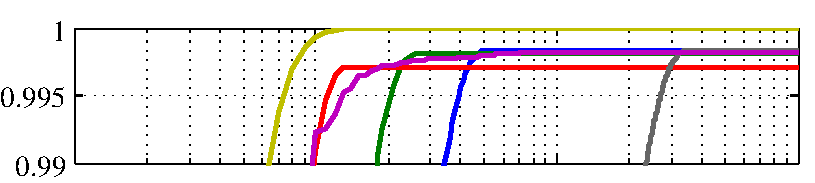
\includegraphics[width=4.34in,clip=true,trim=0in 0in 0.05in 0in]{./figures/compSimZoom}\\
   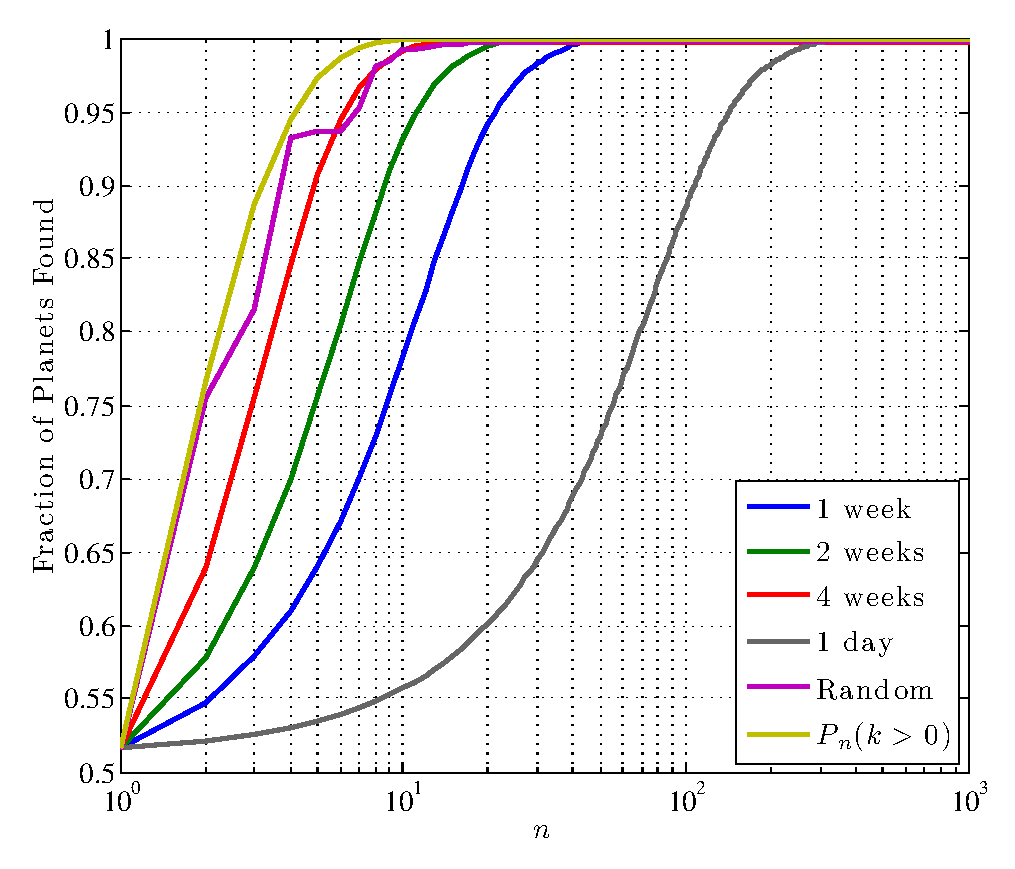
\includegraphics[width=4.5in]{./figures/compSim}
 \end{center}
 \caption[Planet detection probability over multiple visits]{ \label{fig:compSim} 
	The fraction of planets found as a function of number of visits, with various intervals between observations, as well as the bounding probability given by \refeq{eq:multvisit_detprob}.  The curve marked `Random' represents randomized revisit intervals, uniformly distributed within one mean period of the population.  The top panel is a zoomed view of the top 1\% of the plot.}
\end{figure} 

The exception to the bound given by \refeq{eq:multvisit_detprob} would be the case of an optimal observing strategy (i.e., one where we only see previously unobservable portions of the habitable zone on each subsequent visit) on a fully observable system (i.e., one where all parts of the habitable zone are observable at some point).  In the optimal scenario, a new portion of the habitable zone equal to the fraction represented by $p_c$ is observed at each visit and the schedule is such that each portion is observed in sequence so no planets could be bypassed (the equivalent of a continuous observation).  If such an observing schedule could be achieved, the probability of detecting a planet after $1/p_c$ visits would be unity.  For the majority of targets, however, it is quite difficult to follow the strict timing dictated by this strategy.  Because target stars may only be observed for specific intervals of time at given times of the year\footnote{These observable time periods are known as `observing seasons' and are determined by an observatory's keep-out zone, which is discussed in \S\ref{sec:targ_selection}}, it is often impossible to follow the optimal observing schedule in the limited period defined by the mission lifetime.  It is because of these constraints that we often fail to detect existing planets even when the target system has been visited enough times to yield a high probability of detection.  \refeq{eq:multvisit_detprob} always holds as an upper bound for systems with permanently unobservable sections of the habitable zone (where the habitable zone is partially inside the projected IWA).

In the case of only one visit per target star, the calculation of overall detection probability is actually much simpler, and equals the sum of the targets' single visit completeness values.  If all of the targets have the same completeness (fixed $p_c$), then the expected number of planets found ($Y$), given that each star has one ($\eta_\oplus = 1$), is:
\begin{equation}
E[Y] = \sum_{k = 1}^n k \binom{n}{k}  p_c^k (1-p_c)^{n-k} = np_c \,.
\end{equation}
Because $Y$ is the sum of $n$ Bernoulli random variables, each of which has expected value $p_c$, the expected value of $Y$ must be $np_c$.  If the target stars all have different single visit completeness values (non-constant $p_c$), the expected value of $Y$ for $n$ targets with completeness values of $\{p_i\}_{i=1}^n$ is:
\begin{equation}
E[Y] = \sum_{k = 1}^n k  \sum_{j \in \leftsub{n}{C}_k} \prod_{i \in j} p_i  \prod_{i \notin j} (1 - p_i) = \sum_{i = 1}^n{p_i}  \,,
\end{equation}
where $ \leftsub{n}{C}_k$ is the set of combinations of the values from 1 to $n$ taken $k$ at a time.

\section{Analytical Distributions}\label{sec:analytic_dists}
The procedure described in the previous section for generating the completeness function is a Monte Carlo sampling of a bivariate distribution function of non-independent arguments (since star-planet separation and $\Delta$mag are functions of the same parameters).  Thus in order to find any one point (or section) of the completeness distribution, it is necessary to sample it completely.  Because of the relatively high dimensionality of the initial parameter space and wide range of values certain parameters can take, complete sampling requires a large number of Monte Carlo trials.  For example, even with 100 million samples certain low probability areas of the function are significantly under-sampled, as demonstrated in \reffig{fig:undersampled_comp_pdf}.

\begin{figure}[ht]
\centering
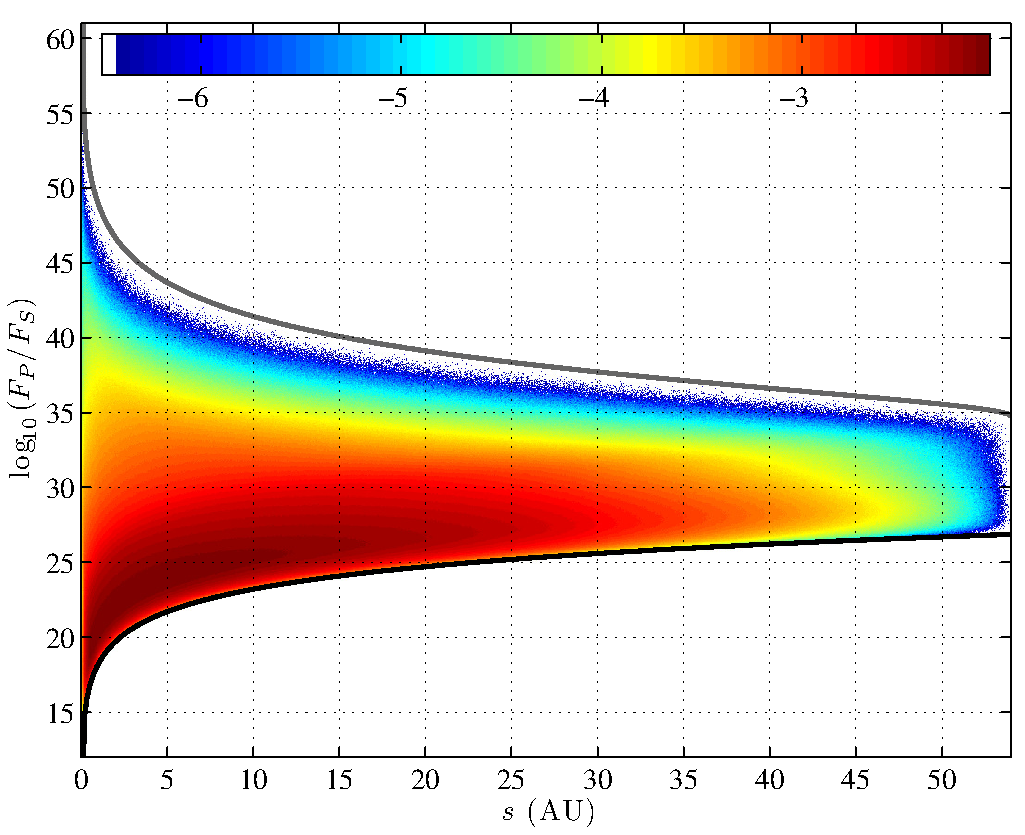
\includegraphics[width=5.5in]{./figures/undersampled_comp_pdf}
 \caption[Undersampled observation PDF]{Observational and photometric completeness for a randomized planetary population  ($a \in [0.4, 30]$, $e \in [0, 0.8]$, $p \in [0.1, 0.5]$, $R \in [0.7, 11.2]R_\oplus$).  The colorbar values and bounding lines are calculated as in \reffig{fig:earthTwin_pdf}. Note that the black line corresponds to high probability areas of the histogram and is thus a good bound, whereas the gray line corresponds to low probability areas and thus demonstrates the undersampling of the Monte Carlo procedure.}
\label{fig:undersampled_comp_pdf} 
\end{figure} 

Any alternate method of sampling the completeness functions introduced in \S\ref{sec:completeness} requires at least some knowledge of their density functions.  In particular, Markov chain methods such as Metropolis-Hastings \citep{hastings1970monte} perform significantly better if the proposal distribution (a function used to `propose' new samples that are then either accepted or rejected) closely approximates the target distribution.  A special case of Metropolis-Hastings, known as Gibbs sampling, can be used to generate a sequence of samples from the joint distribution of two variables if their conditional probabilities are known.  Our goal is to derive the distribution functions of the arguments to the completeness functions.

Following \citet{savransky2011parameter}, we start with an ensemble of Keplerian orbits whose orientation is uniformly distributed in space and derive the distribution functions of these orbits' Keplerian parameters. We make no \emph{a priori} assumptions as to the distribution of orbital semi-major axis and eccentricity, treating them instead as arbitrary functions.  This allows us to derive the completely general distribution functions presented in \S\ref{sec:analytic_dists_deriv}.  A key step here is the demonstration that the planetary phase angle ($\beta$) is independent of any of the orbital parameters.  This makes it possible to write distribution functions for quantities directly related to the two parameters of the direct detection completeness function.  It is important to note that, while the specific application explored here is direct imaging, these distributions are more broadly applicable to exoplanet studies in general.  For example, Keplerian fits are often employed in doppler spectroscopy surveys, making these derivations useful for inferring the true distributions of orbital parameters derived from radial velocity data sets.  Similarly, statistical analyses play an important role in other methods of exoplanet study, including transit photometry and microlensing surveys \citep{gould2010frequency}.

\subsection{Derivation}\label{sec:analytic_dists_deriv}
The distributions of the orbit orienting Euler angles (see \refeq{eq:rpsrot}) are fixed by our assumption of uniform orbital orientation in space.  The remaining two parameters, $a$ and $e$, will be treated as unknowns, with probability density functions (PDFs) $f_{\bar{e}}(e)$ and $f_{\bar{a}}(a)$, respectively. Let $\bar{M}, \bar{e}$ and $\bar{\nu}$ be random variables with the distributions of mean anomaly, eccentricity and true anomaly, respectively, and define two functions: $\nu = g(M,e)$ and $M = h(\nu,e)$.  Following \citet{larson}, we can write the CDF for $\bar{\nu}$ as a marginalization of a conditional probability,
\begin{align} 
F_{\bar{\nu}}(\nu) &= P\left[g(\bar{M},\bar{e}) \le \nu\right] = \int_{-\infty}^{\infty} P\left[g(\bar{M},e) \le \nu | \bar{e} = e\right]f_{\bar{e}}(e)\, \mathrm{d}e\nonumber\\
&=  \int_{0}^{1} P\left[\bar{M} \le h(\nu,e)\right]f_{\bar{e}}(e)\, \mathrm{d}e\,,
\end{align}
where the last step assumes independence between  $\bar{M}$ and $\bar{e}$, and that the orbits are closed so that $e \in [0,1)$.  We note that:
\begin{equation}\label{eq:Mprob}
P[\bar{M} \le h(\nu,e)] = \int_0^{h(\nu,e)} f_{\bar{M}}(M)\, \mathrm{d}M
\end{equation}
where $f_{\bar{M}}(M)$ is the PDF of $M$:
\begin{equation}\label{eq:Mdist}
f_{\bar M}(M) = \left\{
    \begin{array}{l l}
    \frac{1}{2 \pi} & M \; \in \; [0, 2\pi) \\
    0 & \mathrm{else}
    \end{array} \right. \,.
\end{equation}
Therefore the PDF of $\nu$ is:
\begin{equation}\label{eq:nupdf}
f_{\bar{\nu}}(\nu) =  \frac{\mathrm{d}}{\mathrm{d}\nu}F_{\bar{\nu}}(\nu) =  \frac{1}{2\pi} \int_{0}^{1} \frac{\partial h}{\partial \nu}f_{\bar{e}}(e)\, \mathrm{d}e  =  \frac{1}{2\pi} \int_{0}^{1} \frac{\left(1-e^2\right)^\frac{3}{2}}{\left(1+e\cos\nu\right)^2} f_{\bar{e}}(e)\, \mathrm{d}e \, ,
\end{equation}
where $h$ is given by equations (\ref{eq:nutoE}) and (\ref{eq:EtoM}).

Following the same procedure, but without substituting equation (\ref{eq:nutoE}) into equation (\ref{eq:EtoM}), we find that the PDF of the eccentric anomaly is:
\begin{align}
f_{\bar{E}}(E) &=  \int_{0}^{1} \frac{\partial }{\partial E}\left( E - e\sin(E) \right)f_{\bar{M}}(M)f_{\bar{e}}(e)de \nonumber\\
& = \frac{1}{2\pi}\int_{0}^{1} \left(1-e\cos E\right) f_{\bar{e}}(e)\, \mathrm{d}e \,. \label{eq:Edist}
\end{align}
Similarly, if we rewrite the Kepler equation as:
\begin{equation}
M = \cos^{-1}\left(\frac{a - r}{ea}\right) - e\sqrt{1 - \frac{(a-r)^2}{(ea)^2}}
\end{equation}
and assume independence between $\bar a$ and $\bar e$, we can write the PDF for the orbital radius as:
\begin{equation}\label{eq:rpdf}
f_{\bar{r}}(r) = \frac{1}{\pi}\int_{0}^{\infty} \int_{0}^{1} \frac{r}{a\sqrt{(ae)^2 - (a-r)^2}}f_{\bar{e}}(e) \, \mathrm{d}e \, f_{\bar{a}}(a)\, \mathrm{d}a \,.
\end{equation}
Equations (\ref{eq:nupdf}), (\ref{eq:Edist}), and (\ref{eq:rpdf}) are the most complete descriptions possible for the distributions of the orbital position and anomaly, without assuming specific distributions for the eccentricity and semi-major axis.

We derived the distribution functions of the true anomaly and orbital radius by assuming independence between the Keplerian orbital elements from which the anomaly and radius are calculated.  However, the quantities observed by direct searches (i.e., $s$ and $F_R$) are nonlinear functions of the Keplerian elements and $r$, so we cannot make the assumption of independence between their functional arguments for either of these.  Fortunately, inspection of the phase angle reveals something interesting.  Using the approximation in equation (\ref{eq:betadef}), we can write:
\begin{equation}
\beta \approx \cos^{-1}\left(\cos\theta  \cos\nu -\cos\psi  \sin\theta  \sin\nu \right) 
\end{equation}
from which we define a new variable,
\begin{equation} \label{eq:cosBeta}
x \triangleq \cos\beta = \cos\theta  \cos\nu -\cos\psi  \sin\theta  \sin\nu \,.
\end{equation}
If it can be shown that $x$ is uniformly distributed for all distributions of eccentricity, then this would prove that $\beta$ is sinusoidally distributed regardless of the distribution of any other orbital parameter, given only our assumption of uniform orbital orientation.  We do so by considering the characteristic function of $x$,
\begin{equation}
\varphi_{\bar{x}}(t) =  \mathbb{E}\left(e^{i t \bar{x}}\right) = \int_{-\infty}^{\infty} \int_{-\infty}^{\infty} \int_{-\infty}^{\infty} e^{i t x} f_{\bar\nu}(\nu) f_{\bar\psi}(\psi) f_{\bar\theta}(\theta)  \intd{\psi} \intd{\theta} \intd{\nu} \,,
\end{equation}
where $\mathbb{E}$ is the expectation value, and showing that it is equivalent to the characteristic function of a uniformly distributed variable.

The assumption of uniform orbital orientation yields:
\begin{eqnarray}
f_{\bar\psi}(\psi) &=& \left\{
    \begin{array}{l l}
    \frac{1}{2 \pi} & \psi \; \in \; [0, 2\pi) \\
    0 & \mathrm{else}
    \end{array}
    \right. \label{eq:psipdf}\\
f_{\bar\theta}(\theta) &=& \left\{
    \begin{array}{l l}
    \frac{\sin{\theta}}{2} & \theta \; \in \; [0, \pi) \\
    0 & \mathrm{else}
    \end{array}
        \right. \label{eq:thetapdf}
\end{eqnarray}
so that the characteristic function of $x$ becomes:
\begin{equation}
\varphi_{\bar{x}}(t)  = \frac{1}{4 \pi}\int_{-\infty}^{\infty} \int_{0}^{\pi} \int_{0}^{2 \pi}  e^{i t (\cos{\theta}\cos{\nu}- \cos{\psi}\sin{\theta}\sin{\nu})}\intd{\psi} \sin{\theta} \intd{\theta}\, f_{\bar\nu}(\nu) \intd{\nu}
\end{equation}
Performing the integral over $\psi$,
\begin{equation}
    \varphi_{\bar{x}}(t)  = \frac{1}{2}\int_{-\infty}^{\infty} \int_{0}^{\pi}  e^{i t \cos{\theta}\cos{\nu}}  J_{0}\left(t \sin{\theta}\sin{\nu}\right)  \sin{\theta} \intd{\theta}\, f_{\bar\nu}(\nu) \intd{\nu}
\end{equation}
where $J_0$ is the zeroth-order Bessel function of the first kind.
We next perform the integral over $\theta$ using Gegenbauer's finite integral (see equation 12.14(1) in \citet{watson1944treatise}):
\begin{align}
    \int_0^{\pi}  e^{i t \cos{\theta}\cos{\nu}} J_{b-\frac{1}{2}}\left(t \sin{\theta}\sin{\nu}\right) C_a^b{(\cos{\theta})} \sin^{b+\frac{1}{2}}{\theta} \intd{\theta} \nonumber\\
     = \sqrt{\frac{2 \pi}{t}} i^a \sin^{b-\frac{1}{2}}{\nu} \, C_a^b{(\cos{\nu})} J_{a+b}(t)
\end{align}
where $C_a^b$ is a Gegenbauer polynomial.  Choosing $a = 0$ and $b = \frac{1}{2}$ yields $C_a^b(x) = 1$ and the integral becomes:
\begin{equation}
    \int_0^{\pi} e^{i t \cos{\theta}\cos{\nu}} J_{0}\left(t \sin{\theta}\sin{\nu}\right) \sin{\theta} \intd{\theta} = \sqrt{\frac{2 \pi}{t}} J_{\frac{1}{2}}(t)
\end{equation}
Since the half-order Bessel function is defined as:
\begin{equation}
    J_{\frac{1}{2}}(t) = \sqrt{\frac{2}{\pi t}}\sin t
\end{equation}
the characteristic function becomes:
\begin{align}
 \varphi_{\bar{x}}(t)  &= \frac{1}{2} \int_{-\infty}^{\infty} \sqrt{\frac{2 \pi}{t}} \sqrt{\frac{2}{\pi t}}\sin t f_{\bar\nu}(\nu) \intd{\nu} \nonumber\\
&= \frac{\sin t}{t} \int_{-\infty}^{\infty} f_{\bar\nu}(\nu) \intd{\nu} \,.
\end{align}
By definition,
\begin{equation}
\int_{-\infty}^{\infty} f_{\bar\nu}(\nu) \intd{\nu} = 1 \,,
\end{equation}
and thus:
\begin{equation} \label{eq:xChar}
 \varphi_{\bar{x}}(t) = \frac{\sin t}{t} \,.
\end{equation}

If we define a random variable $\bar y \sim U([-1,1])$, its characteristic function will be:
\begin{align}
 \varphi_{\bar{y}}(t) =  \mathbb{E}\left(e^{i t \bar y}\right) &= \int_{-\infty}^{\infty} e^{i t y} f_{\bar y}(y) \intd{y} \nonumber \\
&= \frac{1}{2}\int_{-1}^{1} e^{i t y} \intd{y} = \frac{1}{2}\left(\frac{e^{i t }}{i t} - \frac{e^{-i t }}{i t}\right) \label{eq:uniformChar} \\ 
&= \frac{\sin t}{t} \nonumber \,.
\end{align}
As equations (\ref{eq:xChar}) and (\ref{eq:uniformChar}) are identical, $\bar{x}$ and $\bar{y}$ have the same characteristic function, and thus must have the same underlying distribution.  Since $\bar x$ is uniformly distributed on $[-1, 1]$, $\beta$ is sinusoidally distributed in $[0,\pi)$ for any population of uniformly oriented orbits, independent of the specific distribution of $\bar e$ and $\bar a$.  This finding greatly simplifies our derivation of the distribution functions of the flux ratio and apparent separation.

Returning now to the definition of flux ratio in equation (\ref{eq:fluxRatiodef}), and assuming that we are interested in a particular planet type such that $pR^2$ is approximately constant, we see that the flux ratio is a function of the product of two variables, $m = \Phi(\beta)$ and $n = r^{-2}$.  If we define a random variable $\bar k \triangleq \bar m \bar n$, then it can be shown that:
\begin{equation}\label{eq:distmult}
f_{\bar{k}}(k) = \int_{-\infty}^\infty \frac{1}{n} f_{\bar{m}}\left(\frac{k}{n}\right)f_{\bar{n}}(n)\, \mathrm{d}n
\end{equation}
if $\bar m$ and $\bar n$ are independent \citep{larson}.  As we have demonstrated the independence of $\bar \beta$ from $\bar r$, equation (\ref{eq:distmult}) is applicable.
Using equation (\ref{eq:rpdf}), the CDF of $\bar n$ is given by:
\begin{align}
F_{\bar n}(n) &= P[\bar{r}^{-2} \le n] = P\left[-\frac{1}{\sqrt{n}} \le \bar{r} \le \frac{1}{\sqrt{n}}\right] \nonumber\\
&= \int_{-1/\sqrt{n}}^{1/\sqrt{n}} \frac{1}{2\pi}\int_{0}^{\infty} \int_{0}^{1} \frac{r}{a\sqrt{(ae)^2 - (a-r)^2}}f_{\bar{e}}(e) \, \mathrm{d}e \, f_{\bar{a}}(a)\, \mathrm{d}a \, \mathrm{d}r \\
&= \left. \frac{1}{2\pi}\int_{0}^{\infty} \int_{0}^{1} \sqrt{(ae)^2 - (a-r)^2} + 2 a \tan^{-1}\left(\sqrt{\frac{ae + a - r}{ae - a + r}}\right)\right|_{-1/\sqrt{n}}^{1/\sqrt{n}}\nonumber\\
& \times f_{\bar{e}}(e) \, \mathrm{d}e \, \frac{f_{\bar{a}}(a)}{a}\, \mathrm{d}a \nonumber \,.
\end{align}
The PDF of $n$ is thus:
\begin{align}
f_{\bar n}(n) = \frac{1}{4\pi}\int_{0}^{\infty} \int_{0}^{1}
&n^{-\frac{3}{2}}\left[ \left(C_0 +2a\sqrt{n} - 1\right)^{-\frac{1}{2}} -\left(C_0 - 2a\sqrt{n} - 1\right))^{-\frac{1}{2}}\right] \nonumber\\
& \times f_{\bar{e}}(e) \, \mathrm{d}e \, \frac{f_{\bar{a}}(a)}{a}\, \mathrm{d}a
\end{align}
where $C_0 = a^2(e^2 - 1)n$.  The PDF of $\bar m$ is dependent on the exact form of $\Phi$, but can also be evaluated analytically when $\Phi$ is invertible.  In those cases,
\begin{align}
f_{\bar m}(m) &= f_{\bar \beta}(\Phi^{-1}(m)) \left| \frac{ \mathrm{d}}{ \mathrm{d} m} \Phi^{-1}(m) \right| \label{eq:mpdf}\\
&= 
\left\{
    \begin{array}{c l}
    \frac{1}{2} \sin\left(\Phi^{-1}(m)\right) \left| \frac{ \mathrm{d}}{ \mathrm{d} m} \Phi^{-1}(m) \right|  \quad &  \Phi^{-1}(m) \; \in \; [0, \pi) \\
    0 & \mathrm{else}
    \end{array} \right. \nonumber
\end{align}

This formulation is still problematic when dealing with transcendental functions such as the commonly used phase function of a Lambertian sphere (see \refeq{eq:lambertPhaseFunc}):
\begin{equation}\label{eq:lambertPhase}
\pi \Phi(\beta) = \sin\beta + (\pi - \beta)\cos\beta \, ,
\end{equation}
but, since the domain of the function is restricted to $\beta \in [0,\pi]$, the range of $\Phi$ is single-valued ($\in [1, 0]$), and the function is invertible.  Expanding about $\pi/2$, equation (\ref{eq:lambertPhase}) becomes:
\begin{equation}\label{eq:lambertPhaseSeries}
\Phi(\beta) = \frac{1}{\pi}  + \sum_{k=1}^{\infty} \alpha_k \left(\beta - \frac{\pi}{2}\right)^k \quad\textrm{where}\quad \alpha_k = \frac{d_k}{2 k!}\left(\frac{2 (k-1)}{\pi}\right)^{\frac{d_k + d_{k+1}}{2 d_k}}
\end{equation}
and $d_{1:3} = -1,1,1$, with $d_k = d_{k-1}d_{k-2}d_{k-3}$ for $k > 3$, such that you get the series $d_i = \{-1,1,1,-1,-1,1,1,-1,-1\ldots\}$.  Following \citet{morese1953methods}, we can express the inverse function as the series:
\begin{equation}
\beta = \Phi^{-1}(w) = \frac{\pi}{2}  + \sum_{k=1}^{\infty} b_k \left(w - \frac{1}{\pi}\right)^k 
\end{equation}
where
\begin{equation}
b_k = \frac{1}{k \alpha_1^k} \sum_{x \in X} (-1)^{\vert x \vert} \prod_{r=1}^{\vert x\vert}(k-1+r)  \prod_{i=1}^{k-1}\frac{\left(\alpha_{i+1}/\alpha_1\right)^{x_i}}{x_i!}
\end{equation}
and the space $X$ of sets $x$ is defined as:
\begin{equation}\label{eq:Xspacedef}
X \triangleq \left\{x \in \mathbb{N}^{k-1} : \sum_{i=1}^{k-1} i x_i = k-1\right\} \quad\textrm{with}\quad \vert x\vert \triangleq \sum_i x_i \,.
\end{equation}
The inverse series converges to machine double precision in a finite number of terms, except at the endpoints (0 and 1), which themselves do not need to be computed as they map exactly to $\beta = \pi$ and $\beta = 0$, respectively.

Since $\bar F_R = pR^2 \bar k$, Equations (\ref{eq:distmult}) - (\ref{eq:Xspacedef}) allow us to write:
\begin{align}
f_{\bar F_R}(F_R) = \frac{1}{pR^2}\int_{-\infty}^\infty \frac{f_{\bar{n}}(n)}{n} & \cos\left(\sum_{k=1}^{\infty} b_k \left(\frac{F_R}{npR^2} - \frac{1}{\pi}\right)^k\right)\nonumber\\
&\times \left|\sum_{k=1}^\infty k b_k \left(\frac{F_R}{npR^2} - \frac{1}{\pi}\right)^{k-1} \right| \, \mathrm{d}n \label{eq:FRpdf} \,,
\end{align}
which represents the PDF of the planet-star flux ratio for a population of planets with constant $pR^2$ values (i.e., Earth-twins) modeled as Lambertian reflectors.

While \refeq{eq:FRpdf} is computationally tractable and produces accurate results, the coefficient sets in \refeq{eq:Xspacedef} can be very time consuming to compute when a large number of terms is required for convergence.  This leads us to consider a purely numerical solution that nonetheless produces equally accurate results.  Rather than using series reversion, we can use an iterative numerical method to invert $\Phi(\beta)$ and then calculate the first order derivative of the result via finite differences.  Recalling the definition of $m$, by which $\beta = \Phi^{-1}(m)$, we select an initial value for $\beta$ by fitting and inverting a cubic polynomial to $m = \Phi(\beta)$, resulting in:
\begin{equation}\label{eq:betaCubicEst}
\beta_0 = -5.921m^3+ 9.825m^2 - 6.636m + 2.802
\end{equation}
when $\Phi$ is the Lambert phase function.  Next, we use Newton-Raphson iteration to update the estimate as:
\begin{equation}
\beta_{n+1} = \beta + \frac{1}{\pi - \beta}\left(1 + \frac{\pi - \beta}{\tan\beta}  -  \frac{\pi m}{\sin\beta}\right) \,.
\end{equation}
This function, using the initial estimate in \refeq{eq:betaCubicEst}, converges to machine double precision within 25 iterations for all values of $\beta$, except for the endpoints, which can be simply substituted for their correct values as described above.  By using sufficiently small step sizes, the error produced by estimating the derivative via finite differences can similarly be constrained.

When the number of terms leading to convergence is relatively small (on the order of 50), the space $X$ can be calculated in its entirety.  This is done by first recursively generating all of the unique sets of natural numbers of length $k-1$ that sum to $k-1$.   We generate all of the unique pairs of values that sum to $k-1$, and then recursively augment these sets with all of the sets that sum to the value of the last set element, until no new combinations can be generated.  These sets are encoded as an $N \times k-1$ matrix, where $N$ is the number of unique combinations. For each  entry of this matrix of \emph{value} $i$ (where $i \ne 0$) in the $j$th row, the entry in the $j$th row and $i$th column of a matrix of equivalent size is iterated by one.  The result is a matrix encoding the entire space $X$ in its rows.  This basic process is quite computationally intensive (of order $n^n$), but can be made significantly more efficient by removing redundant sets at every iteration of the recursive set generation, and by employing an efficient sort when filling the final matrix, rather than doing so recursively.  These improvements greatly decrease the computational complexity, bringing the running time down to order $2^n$.  A sample implementation that is capable of generating $X$ for $k-1 = 45$ ($N = 89134$) in under 2 minutes on a single core is presented in \refcode{code:calcRevCoefs}.

Finally, we consider the apparent separation.  The same approximation used in equation (\ref{eq:betadef}) allows us to write:
\begin{equation}
s = r \sin \beta \,.
\end{equation}
If we let $\bar l = \sin\bar\beta$, following equation (\ref{eq:mpdf}):
\begin{equation}\label{eq:lpdf}
f_{\bar l}(l) = f_{\bar \beta}(\sin^{-1}(l)) \left| \frac{ \mathrm{d}}{ \mathrm{d} l} \sin^{-1}(l) \right| = 
\left\{
    \begin{array}{l l}
    \frac{l}{\sqrt{1 - l^2}} & l \; \in \; [0,1) \\
    0 & \mathrm{else} \end{array}\right.
    \end{equation}
Returning to equations  (\ref{eq:rpdf}) and (\ref{eq:distmult}) and now letting $\bar m = \bar r$ and $\bar n = \bar l$, we have:
\begin{equation}\label{eq:spdf}
f_{\bar s}(s) = \frac{1}{\pi}  \int_{0}^1 \int_{0}^{\infty} \int_{0}^{1} \frac{s}{a\sqrt{\left(1 - l^2\right)\left[(ael)^2 - (al-s)^2\right]}}f_{\bar{e}}(e) \, \mathrm{d}e \, f_{\bar{a}}(a)\, \mathrm{d}a \, \mathrm{d}l  \, ,
\end{equation}
which represents the probability density function of the apparent separation.  We now have expressions for the distribution functions of both of the observed quantities of direct imaging planet searches.  While the expressions are quite complex, they are numerically integrable, and can be used to check and improve the efficiency of the sampling of the completeness function.   With an assumed $f_{\bar e}(e)$ and $f_{\bar a}(a)$, equations (\ref{eq:FRpdf}) and (\ref{eq:spdf}), via marginalization and joint sampling, can directly produce the completeness distribution.

\subsection{Validation}
As a check on the derived distribution functions for the true anomaly and orbital radius, we first consider the simplest possible case, where both eccentricity and semi-major axis are uniformly distributed:
\begin{eqnarray}
f_{\bar e}(e) &=& \left\{
    \begin{array}{l l}
   1 & e \; \in \; [0, 1] \\
    0 & \mathrm{else}
    \end{array}
    \right. \label{eq:euniformpdf}\\
f_{\bar a}(a) &=& \left\{
    \begin{array}{l l}
    (a_{max} - a_{min})^{-1} &a \; \in \; [a_{max}, a_{min}] \\
    0 & \mathrm{else}
    \end{array}
        \right. \label{eq:auniformpdf}
\end{eqnarray}
Equation (\ref{eq:nupdf}) then becomes:
\begin{align} \label{eq:nupdfuniform}
f_{\bar{\nu}}(\nu) &=  \frac{1}{2\pi} \int_{0}^{1} \frac{\left(1-e^2\right)^\frac{3}{2}}{\left(1+e\cos\nu\right)^2}\, \mathrm{d}e  \nonumber \\
&= -{}_2F_1(1,2;7/2,\cos^2\nu)\frac{\cos\nu}{5\pi} - \frac{3}{16 \cos^4\nu}\left(4\sin\nu + \cos 2\nu - 3\right)
\end{align}
where ${}_2F_1$ is the Gaussian hypergeometric function:
\begin{equation}\label{eq:gaussHyper}
{}_2F_1(a,b;c;z) = \sum_{k=0}^\infty \frac{(a)_k (b)_k}{(c)_k} \frac{z^k}{k!} \,,
\end{equation}
with the Pochhammer symbol $(\cdot)_k$ defined as:
\begin{align}
(x)_0 &= 1 \,,\\
(x)_k &= \prod_{n=0}^{k-1} (x+n) \,,
\end{align}
and with the value of $c$ limited to the set of natural numbers, i.e., $ c \in  \mathbb{Z}^+ \backslash \left\{0\right\}$.  Equation (\ref{eq:rpdf}) becomes:
\begin{align}
f_{\bar{r}}(r) =\frac{1}{\pi a \left(a_{max} - a_{min}\right)} 
& \left[ 2 r \log\left(\frac{\sqrt{a - r} + \sqrt{r - a}}{\sqrt{2a - r} + \sqrt{r}}\right) \right. \nonumber\\
& {} + a\log\left(a - r\right)+ 2a\log\left(-2\left(r + \sqrt{2ar - r^2}\right)\right)  \label{eq:rpdfuniform}  \\
&  \left.\left.{} + ia\log\left(\frac{32r\left(r - a + i\sqrt{(2a - r)r}\right)}{a}\right) \right]\right|_{a_{min}}^{a_{max}} \nonumber \, .
\end{align}

To check these equations, we generate one million IID samples each from the uniform distributions in Equations (\ref{eq:euniformpdf}), (\ref{eq:auniformpdf}) and (\ref{eq:Mdist}) \citep{press1992numerical}.  From these, we calculate the eccentric anomalies via Newton-Raphson iteration applied to \refeq{eq:EtoM}, and then calculate $\nu$ and $r$ via Equations (\ref{eq:nutoE}) and (\ref{eq:rdef}), respectively (see \S\ref{sec:gen_plan_sys}, Equations (\ref{eq:NewtonRaphson}) - (\ref{eq:E0selection})).  The sample PDFs are calculated  for these two parameters and compared with the results of our closed-form solutions, as shown in Figures \ref{fig:compDistsa} and \ref{fig:compDistsb}.  These plots demonstrate excellent agreement, validating the equations. 

\begin{figure}[ht]
\centering
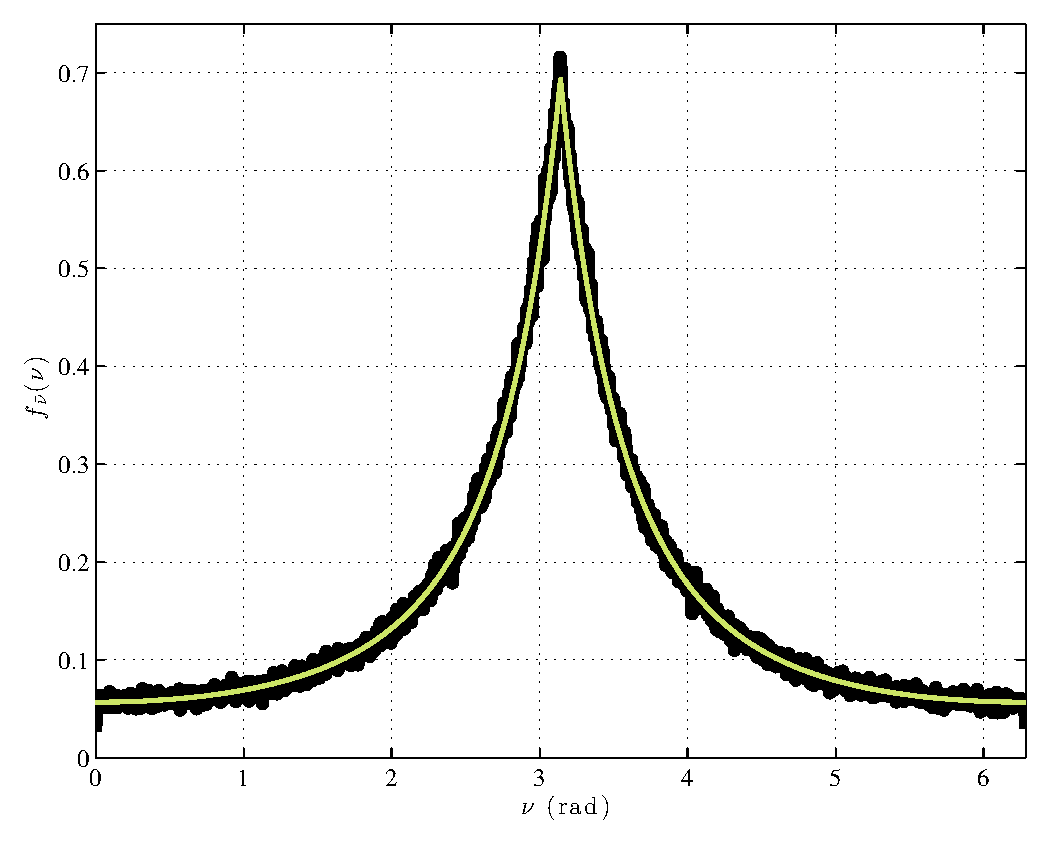
\includegraphics[width=5in]{./figures/compDistsa}
 \caption[Validation of analytical $\nu$ PDF]{ Comparison of empirical (black line) and derived (green line) values of $f_{\bar{\nu}}$ assuming a uniform distribution for $\bar e$. \label{fig:compDistsa}}
\end{figure}  

\begin{figure}[ht]
\centering
\subfigure[$f_{\bar{r}}$, uniform $a$]{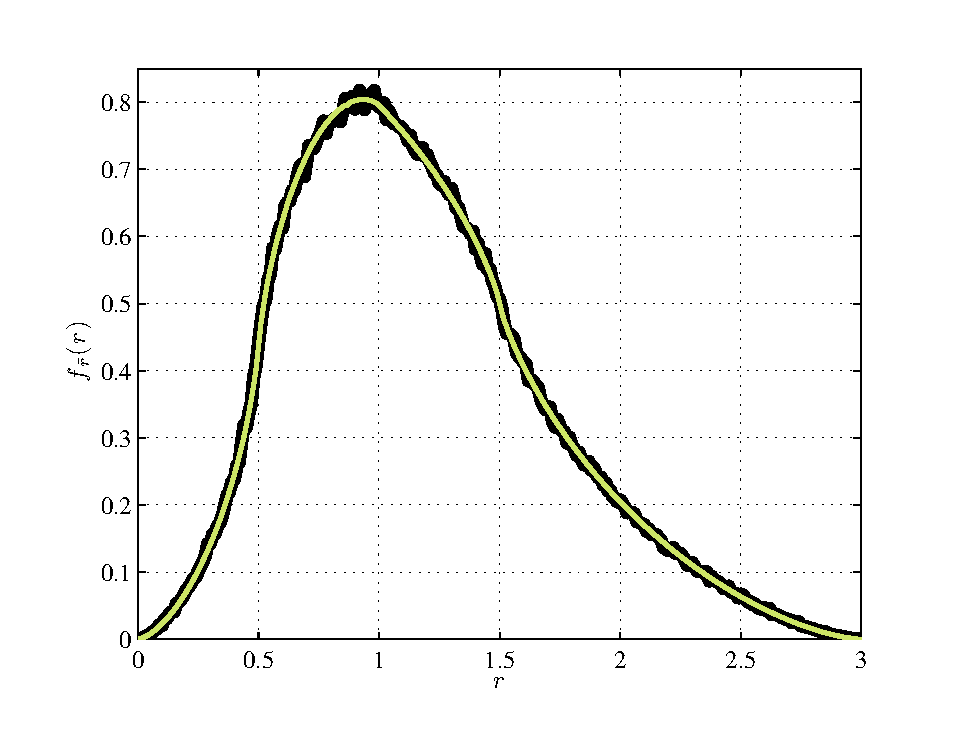
\includegraphics[width=2.95in,clip=true,trim=0.3in 0.1in 0.5in 0.3in]{./figures/compDistsb}\label{fig:compDistsb}}
\subfigure[$f_{\bar{r}}$, log $a$]{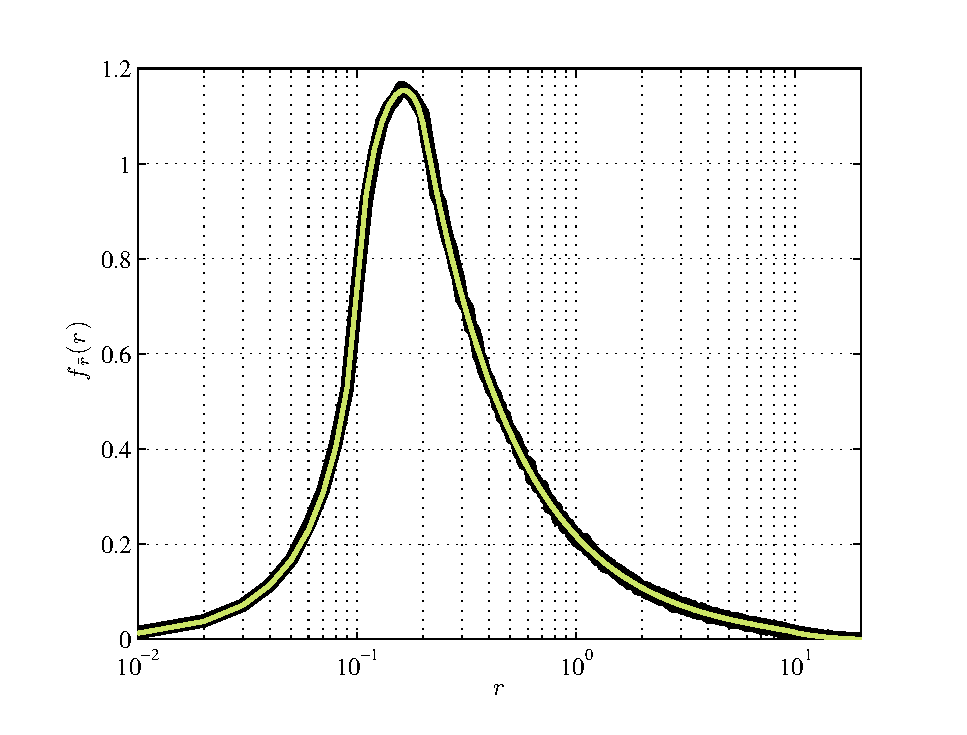
\includegraphics[width=2.95in,clip=true,trim=0.3in 0.1in 0.5in 0.3in]{./figures/compDistsc}\label{fig:compDistsc}}
 \caption[Validation of analytical$r$ PDFs]{ Comparison of empirical (black line) and derived (green line) values for  $f_{\bar{r}}$, assuming a uniform distribution for $\bar e$ and uniform and log distributions for $\bar a$.  For uniformly distributed semi-major axis we have $a \in [0.5, 1.5]$, leading to $r \in (0, 3]$, and for $\bar a$ uniform in $\log a$, we have $a \in [0.1, 10]$ leading to $r \in (0, 20]$. \label{fig:compDists}}
\end{figure}  

While uniform distributions are a useful check, the semi-major axes of currently found planets appear more likely to be logarithmically distributed \citep{currie2009semimajor}. As an additional test, we will assume that $\bar a$ is uniformly distributed in $\log_{10}(a)$ for $a \in [10^{c_{min}}, 10^{c_{max}}]$ so that its PDF is:
\begin{equation}\label{eq:alogpdf}
f_{\bar a}(a) = \left\{
    \begin{array}{l l}
    \left(\Delta c\log(10) a\right)^{-1} &a \; \in \;  [10^{c_{min}}, 10^{c_{max}}]\\
    0 & \mathrm{else}
    \end{array}
        \right.
\end{equation}
where $\Delta c = c_{max} - c_{min}$.
If we retain the same uniform distribution for eccentricity, the true anomaly distribution remains the same, but the orbital radius density becomes:
\begin{align}
f_{\bar{r}}(r) =\frac{1}{2\pi \log(10)\Delta c a^2 r} 
& \left[a\sqrt{(2a - r)r} - a^2\log\left(a - r\right)\right.\nonumber\\
&{} - 2ia^2\log\left(\frac{32 r^3}{a}\left(r - a i \sqrt{(2a - r)r}\right)\right) \nonumber\\
& {} + 2a^2\log\left(-4\left( \sqrt{(2a - r)r^3} + r^2\right)\right)\label{eq:rpdflog}\\
&\left.\left.{} + 2r^2\log\left(\frac{\sqrt{a - r} - \sqrt{r-a}}{\sqrt{2a - r} + \sqrt{r}}\right)\right]\right|_{10^{c_{min}}}^{10^{c_{max}}}\nonumber \, .
\end{align}
We repeat the simulation, this time generating our sample of semi-major axes by exponentiating 10 with a sample of one million uniformly distributed random values between -1 and 1 (thereby setting $\Delta c$ to 2), and re-calculating the PDF for $f_{\bar r}$.  This is compared with the results from \refeq{eq:rpdflog} in \reffig{fig:compDistsc}, and shows excellent agreement.

We can also empirically check the assertion that the distribution of $\beta$ is independent of the distribution of $\bar e$.  We now generate two sets of IID samples, one using the uniform distribution of $\bar e$, and one distributed via a step function,
\begin{equation}\label{eq:piecewise_fe}
f_{\bar e}(e) = \left\{
    \begin{array}{l l}
   1.3 & e \; \in \; [0, 0.7) \\
   0.3 & e \; \in \; [0.7, 1]\\
    0 & \mathrm{else}
    \end{array}
    \right.
\end{equation}
where accurate sampling is achieved via simple rejection sampling.  The two sample sets are used to generate two different sample distributions of $\bar\beta$.  Figure \ref{fig:qqplots} shows Q-Q plots comparing the quantiles of these two samples to the theoretical quantiles of a sinusoidal distribution.  Quantiles for the ideal sinusoidal distribution are calculated by evaluating its inverted CDF at regularly spaced intervals, while quantiles of the two simulated distributions are calculated by ordering and binning the generated values.  As the resulting Q-Q plots follow the 45$^\circ$ line, this demonstrates that the simulated distributions are identical to the theoretical sinusoidal distribution \citep{gibbons2003nonparametric}.
 \begin{figure}[ht]
\centering
\subfigure[Uniform $f_{\bar{e}}$]{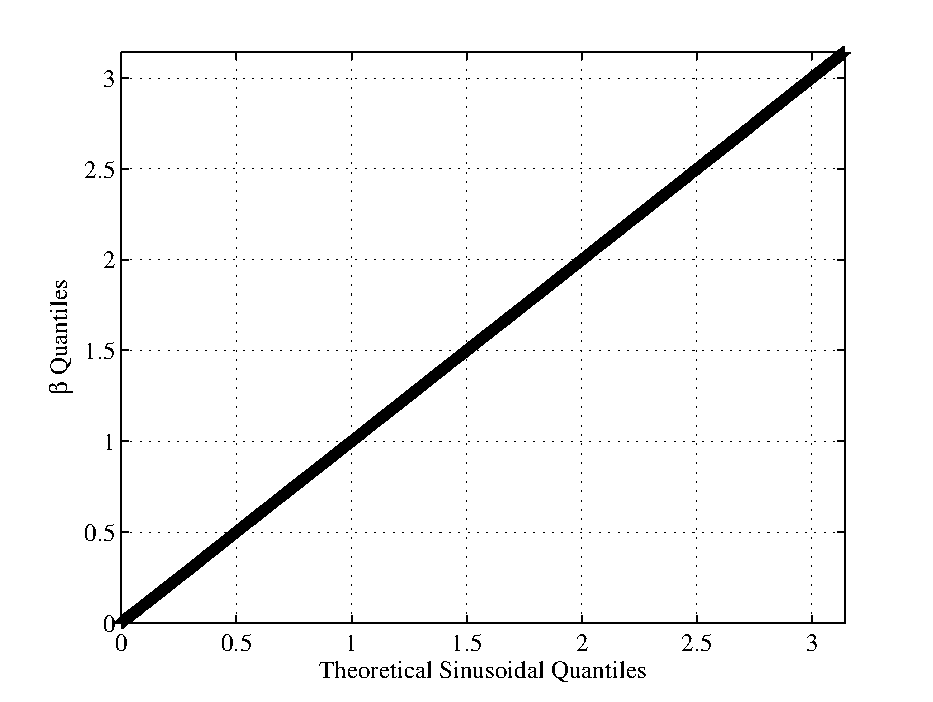
\includegraphics[width=2.95in,clip=true,trim=0.3in 0.1in 0.5in 0.3in]{./figures/qqplota}}
\subfigure[Step $f_{\bar{e}}$]{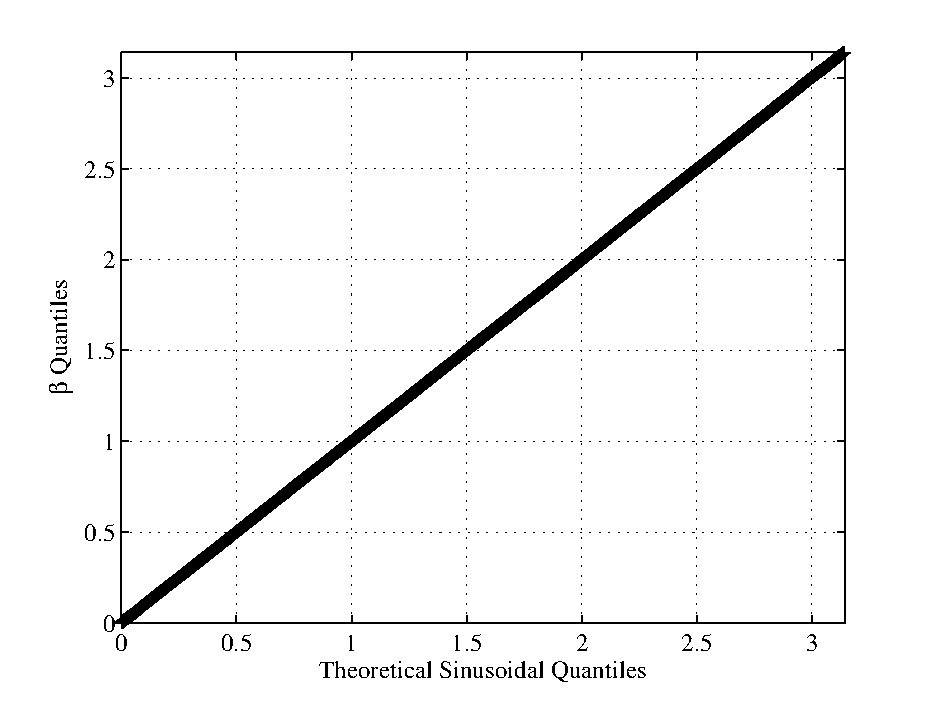
\includegraphics[width=2.95in,clip=true,trim=0.3in 0.1in 0.5in 0.3in]{./figures/qqplotb}}
 \caption[$f_{\bar\beta}$ Q-Q plots]{ Q-Q plots of empirically derived $f_{\bar\beta}$ distributions compared with theoretical sinusoidal quantiles. \label{fig:qqplots}}
\end{figure}

Continuing on to the analytical distributions of the direct detection observables, \refeq{eq:mpdf} allows us to find the PDF of the Lambert Phase function, as shown in \reffig{fig:mdist}.  Similarly, we can use \refeq{eq:spdf} to find the PDF of the apparent separation via quadrature as shown in \reffig{fig:sint}.
\begin{figure}[ht]
\centering
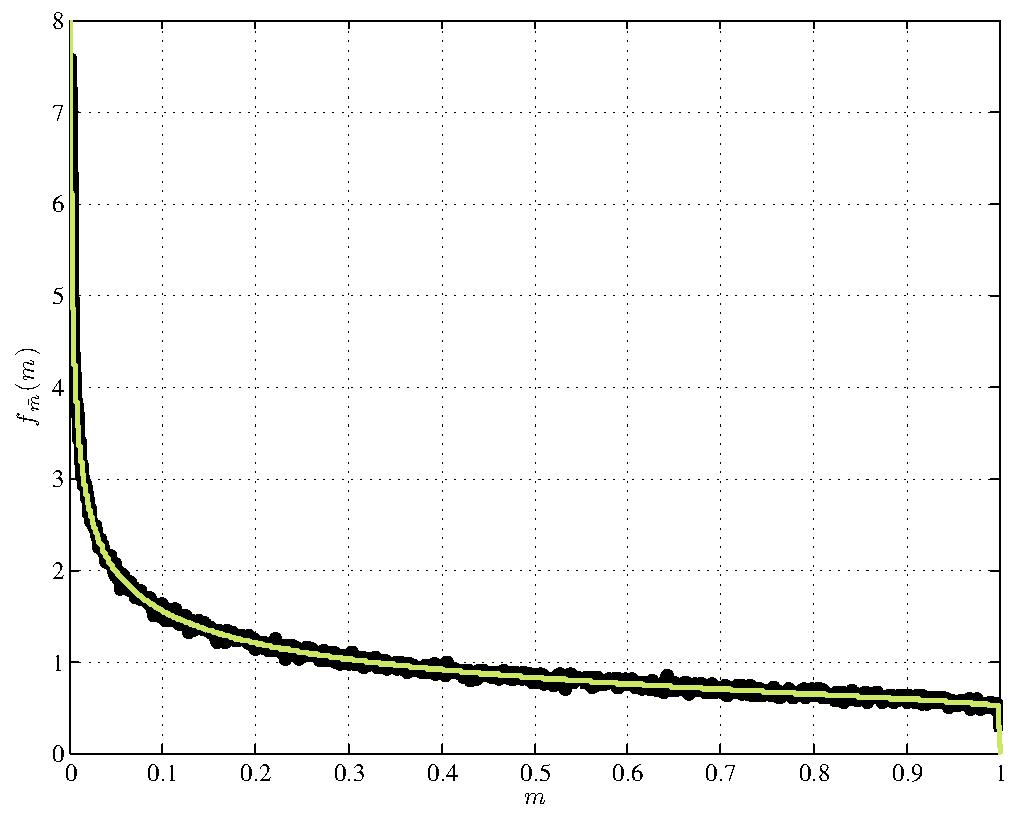
\includegraphics[width=5in]{./figures/mdist}
\caption[Validation of analytical $m$ PDF.]{ Comparison of empirical (black line) and derived (green line) distributions for the Lambert phase function $m = \Phi(\beta)$ for sinusoidally distributed $\beta$. Note that in the derived distribution, the endpoints go to zero and infinity, behavior that is not captured in the empirical distribution. \label{fig:mdist}}
\end{figure}  
\begin{figure}[ht]
\centering
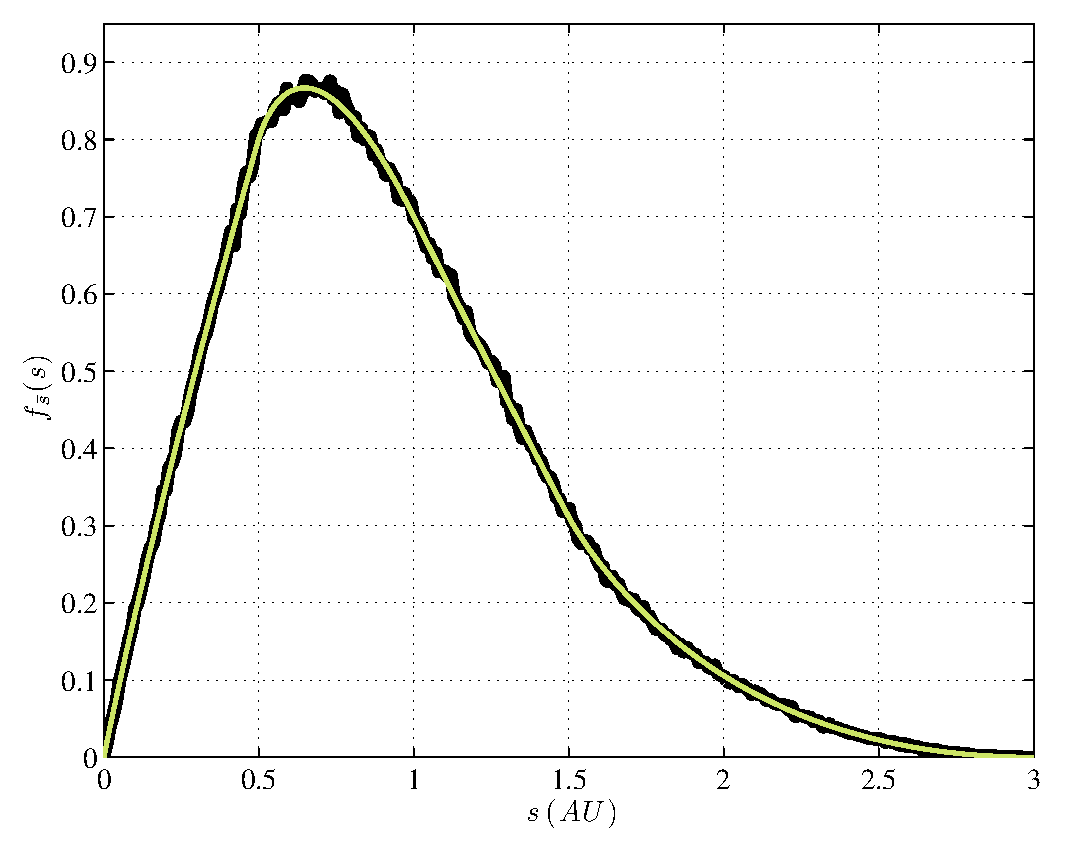
\includegraphics[width=5in]{./figures/sint}
\caption[Validation of analytical $s$ PDF.]{ Comparison of empirical (black line) and derived (green line) distributions assuming the uniform distribution for $\bar e$ and $\bar a$ used in \reffig{fig:compDistsb}. \label{fig:sint}}
\end{figure}

\subsection{Applications}
In addition to improving our ability to sample the completeness function, these analytical distributions have multiple other applications.  One particularly interesting question is how we can use these forms to extract more information from observations and improve overall observing efficiency.  For example, \refeq{eq:spdf} can be used to provide us with information about an orbit's semi-major axis from measurements of apparent separation.  Given a set of measurements of the apparent separation $\left\{s_i\right\}_{i = 1}^n$, the maximum likelihood estimate (MLE) for $a$ is given by \citep{ogunnaike2009random}:
\begin{equation}
\hat a = \arg\max_{a \in \bar a} \hat \ell \left(a \vert s_{1\ldots n}\right)
\end{equation}
where $\hat \ell$ is the likelihood function generally given as:
\begin{equation}
\hat l\left(\theta\vert x_{1\ldots n}\right)= \log f\left(x_{1\ldots n} \vert \theta\right)/n \, .
\end{equation}
Rewriting \refeq{eq:spdf}:
\begin{align}
f_{\bar s}(s) &= \int_a f_{\bar s\vert\bar a}\left(s \vert a\right)f_{\bar{a}}(a)\, \mathrm{d}a\\
& =  \int_{0}^{\infty}\frac{1}{\pi}  \int_{0}^1  \int_{0}^{1} \frac{s}{a\sqrt{\left(1 - l^2\right)\left[(ael)^2 - (al-s)^2\right]}}f_{\bar{e}}(e) \, \mathrm{d}e \, \mathrm{d}l  \,  f_{\bar{a}}(a)\, \mathrm{d}a \nonumber
\end{align}
so that
\begin{equation}
 f_{\bar s\vert\bar a}\left(s \vert a\right)  = \frac{1}{\pi}  \int_{0}^1  \int_{0}^{1} \frac{s}{a\sqrt{\left(1 - l^2\right)\left[(ael)^2 - (al-s)^2\right]}}f_{\bar{e}}(e) \, \mathrm{d}e \, \mathrm{d}l  \,.
\end{equation}
Since the logarithm is a monotonic function, for a single observation of the apparent separation $s = s_0$, the MLE for semi-major axis is therefore:
\begin{equation}\label{eq:aMLE}
\hat a = \arg\max_{a \in \bar a}   \frac{1}{\pi}  \int_{0}^1  \int_{0}^{1} \frac{s_0}{a\sqrt{\left(1 - l^2\right)\left[(ael)^2 - (al-s_0)^2\right]}}f_{\bar{e}}(e) \, \mathrm{d}e \, \mathrm{d}l \,.
\end{equation}

It is clear that the value of $a$ maximizing this equation is equal to $s_0$---i.e., the likeliest value for the semi-major axis given a single observation of the apparent separation is the apparent separation itself, as demonstrated in \reffig{fig:amle}.  Note that the apparent separation can be less than the semi-major axis due to either orientation of the orbit with respect to the line of sight or the orbit's eccentricity.  The apparent separation can be greater than the semi-major axis due only to eccentricity.  As multiple observations of a single exosystem cannot be treated as independent, subsequent measurements of the apparent separation cannot be introduced into the likelihood estimator in \refeq{eq:aMLE}, but may be included in orbital fits.  Nevertheless, the likelihood function can be used to weight each individual observation, and this estimator proves highly useful in the area of mission planning and observation scheduling, as will be discussed in \S\ref{sec:scheduling}.
\begin{figure}[ht]
\centering
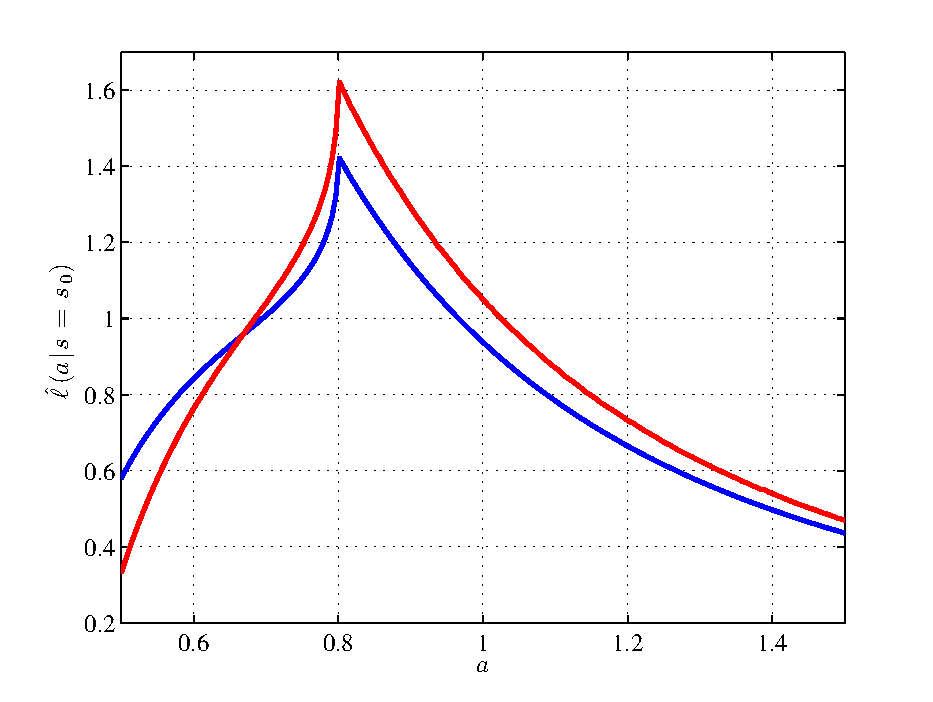
\includegraphics[width=5.5in]{./figures/amle}
\caption[Maximum likelihood for $a$ given $s$.]{Likelihood function for semi-major axis given one observation of apparent separation $s_0 = 0.8$.  $a$ is uniformly distributed $\in [0.5, 1.5]$ and $e$ is distributed either uniformly (blue line) or as in \refeq{eq:piecewise_fe} (red line).  In each case, the value of $a$ maximizing the likelihood function is equal to $s_0$. \label{fig:amle}}
\end{figure}

Returning to the description of transit photometry in \S\ref{sec:photometry}, we see from \refeq{eq:transitFe} that a transit can also be defined in terms of the apparent separation.  In fact, in the simplest possible treatment we can define a generalized transit condition of:
\begin{equation}\label{eq:transitCondition}
s < R_S + R \,.
\end{equation}
Of course, this includes transits that are merely grazing and beyond the sensitivity of available instruments, so the subset of detectable transits is determined by the magnitude of the brightness variation ($F^{(e)}_S/F_S$), just as with direct detections.  However, if we wish to calculate the overall probability of any transit occurring at any point in time, we can simply wirte:
\begin{equation}
P\left[s < R_S + R\right] = \int_0^{R_S + R} f_{\bar s} (s) \intd{s} \,.
\end{equation}
Furthermore, if we consider a particular population of orbits---for example, circular orbits with semi-major axis $a_0$---this further simplifies to:
\begin{equation}
\begin{split}\label{eq:instTransitProb}
P\left[s < R_S + R| a=a_0, e=0\right] &= \int_0^{R_S + R} f_{\bar s} (s) \intd{s} \\
&= \frac{1}{\pi} \int_0^{R_S + R}  \int_{0}^1  \frac{s}{a_0\sqrt{\left(1 - l^2\right)(al-s)^2}} \intd{l} \intd{s}\\
 &= \frac{(R_S + R)^2}{2\pi a_0} \,.
\end{split}
\end{equation}

\begin{figure}[ht]
\centering
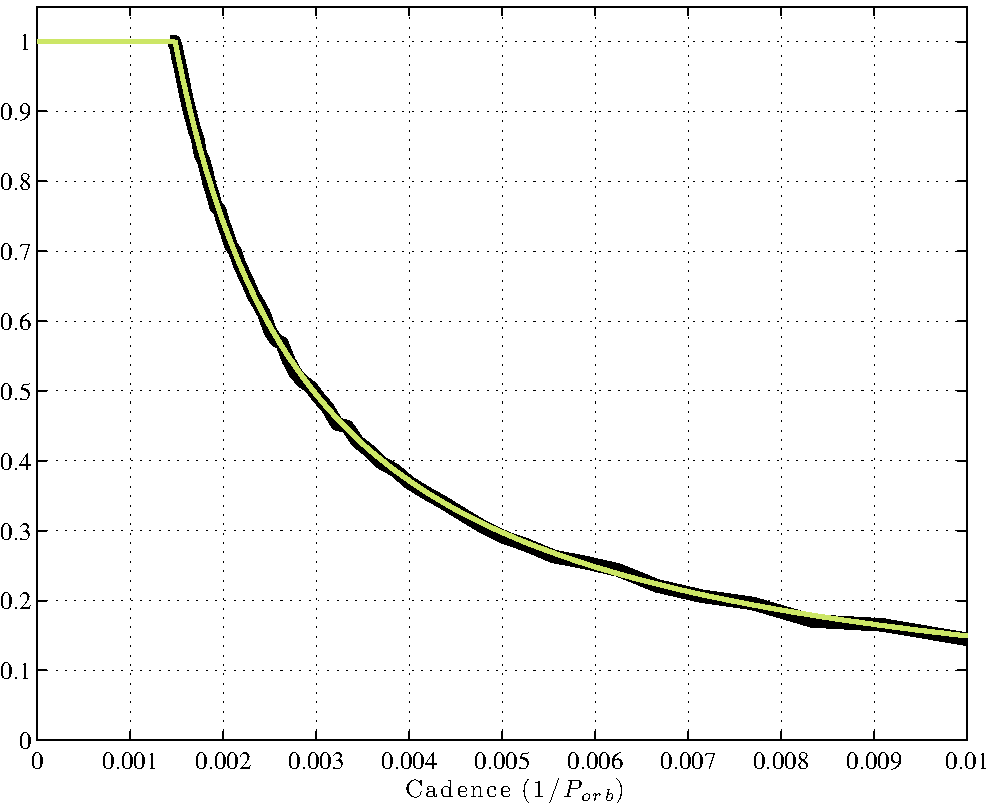
\includegraphics[width=5in]{./figures/transitCadences}
\caption[Portion of observable transits detected over one period.]{Portion of observable transits detected over one orbital period for $a_0 = 1, R_S = R_\odot$ and $R = 0$ as a function of observation cadence. The black line represents the results of simulating one million planets on orbits where transits would occur ($\vert \theta \vert  < R_s/a_0$) and propagating them forward in time by varying time steps.  The green line is defined by \refeq{eq:transitCadenceDropoff}.
\label{fig:transitCadences}}
\end{figure}
While an interesting result, \refeq{eq:instTransitProb} is not very useful on its own, as it represents an instantaneous probability of transits, whereas we are generally interested in the probability of transits over a certain time period (for example, one of the Kepler quarters \citep{borucki2010kepler}).  Every transit photometry survey has a certain cadence of observations as even instruments that monitor stars continuously have a finite integration and readout time.  Therefore, we can model transit observations on a large group of stars as a Poisson process.  While the occurrence of transits about a single star is not independent, if we are merely interested in the portion of monitored stars that will have at least one transit in a given period of time, then we have a collection of random variables representing the number of events occurring throughout a given time interval, each of which is Poisson distributed.  Thus, the portion of target stars with detected transits is a monotonically increasing function in time, with each specific interval having a probability of non-zero transits of:
\begin{equation}
P[N(\Delta t) > 0] = 1 - e^{-\lambda \Delta t} \,
\end{equation}
where $\Delta t$ is the time interval and $\lambda$ is the expected number of occurrences per interval.  This formulation, along with \refeq{eq:instTransitProb}, allows us to calculate the optimal cadence such that 100\% of transits could be captured within one orbital period:
\begin{equation}\label{eq:optimalTransitCadence}
\Delta t_0 = \frac{1}{\pi} \frac{R_s + R}{a_0}
\end{equation}
where this value is in units such that the orbital period associated with $a_0$ (for zero planet mass) is 1.  For any greater time step, the portion of transits discovered within one orbital period is given by:
\begin{equation}\label{eq:transitCadenceDropoff}
\frac{N(\Delta t)}{N(\Delta t_0)} = \frac{\Delta t_0}{\Delta t} + \Delta t \,.
\end{equation}

Of course, the actual portion of transits detected will always be less than unity due to the photometric limitations of the instrument, but the sampling rate in \refeq{eq:optimalTransitCadence} represents the optimal cadence for a given semi-major axis.  Since this interval is inversely proportional to semi-major axis, studies interested in closer-in planets can actually monitor stars fairly infrequently, whereas those looking for further out planets must monitor nearly continuously (as is evident from the geometry of the problem).  \reffig{fig:transitCadences} shows a comparison of  Equations (\ref{eq:optimalTransitCadence}) and (\ref{eq:transitCadenceDropoff}) with results from simulation, demonstrating excellent agreement.

\bigskip
\bigskip

The specific detection method biases, the statistical modeling of exoplanet populations and the concept of completeness are all extremely important to both observation simulation and data analysis.  The next two chapters will demonstrate this using the framework developed here, including the observation timing optimizations.  \refch{ch:obs_sims} will present the details of constructing a planet-finding mission simulation, many of which deal with observation scheduling and are thus greatly informed by completeness and the distributions of planetary parameters. 
 % Dists
\chapter{Observation Simulation}\label{ch:obs_sims}

Along with improvements in instrumentation and data analysis, the planet-finding community has also devoted resources to the development of detailed models and simulations of the various instruments and surveys currently in operation.  These simulations serve three main purposes:  first, they allow the community to directly compare the expected scientific returns of proposed observatory and mission concepts \citep{savransky2010}.  Second, these simulations can be used to optimize target selection and observation scheduling for existing facilities, and provide a controlled testing environment for data processing pipelines \citep{bryson2010kepler}. Finally, by simulating a planet population derived from a specific formation/evolution theory, we can estimate the likelihood of survey results, and thus accept or reject the theory, while also closely estimating absolute planet frequencies \citep{gould2010frequency}.  This last capability translates to the ability to use surveys as controlled experiments to choose between competing exosystem formation and evolution theories.  The ability to predict the expected science returns of a proposed architecture is particularly important given the resources required to operate a major ground-based observatory, or to launch a new space observatory.  

A satellite along the lines of the Hubble Space Telescope or James Webb Space Telescope is a major undertaking and should only be built if it has a reasonable chance of succeeding in its stated mission.  In terms of mission planning and design, this translates to formulating a set of requirements which are reasonable given our current state of knowledge, and then designing hardware which will meet these requirements.  This chapter will present the techniques required to model whole planet-finding missions and surveys, as well as a selection of case studies demonstrating various applications of these methods.

\section{Mission Planning and Analysis}\label{sec:ch4_intro}

There are two possible approaches to predict scientific performance of potential planet finding missions.  The first is to use a numerically evaluated statistical description of various quantities involved in a planetary detection and report results in terms of expected values  of random variables, producing either an expected number of planets found as in \citet{brown2005}, or a total number of zones of interest probed\footnote{A zone of interest refers to the fractional volume of space that is observed in the course of the mission where a planet of interest might reside.} as in \citet{lindler2007}.  While these are powerful metrics for mission performance, they make it very difficult to evaluate highly specific mission requirements.  For example, if we wish to require that our instrument produce orbital fits for $m$\% of all planets found such that the fit eccentricities will be within $n$\% of their true values, the statistical description of this requirement would be quite complex.  The second option is to perform an analysis in which we simulate the entire mission, along with all detections, many times over, which allows us to not only evaluate the requirement above, but also actually produces values for $n$ and $m$ for every evaluated design.  By performing such simulations many times over, with varying populations of planets, we produce an ensemble of mission timelines, giving us distributions of mission science yields. While this approach is significantly more computationally intensive than earlier treatments, it has the advantage of allowing us to answer a variety of questions about proposed mission architectures with a single ensemble of simulations.

In addition to helping us decide what exactly to fund, construct, and fly, this Monte Carlo approach has an additional benefit.  A complete simulation capability of planet finding missions will not only allow us to compare the performance of different instrument designs, but also different mission designs for the same instrument.  Assuming sufficient faith in the accuracy of the simulation, we can evaluate strategies and rules before any hardware is even assembled. Additionally, once a robust simulation framework has been constructed, it becomes quite simple to answer additional questions.  A wholly analytical approach would require at least a partial reformulation of the problem before we could tell, for example, what effect knowing exactly which stars have planets would have on the mission results, but a Monte Carlo approach can give us the answer simply by running another set of simulations.  The mission analysis method detailed in this chapter was first presented in \citet{savransky2008} and further developed in \citet{savransky2010}.  It involves generating randomized planetary systems assigned to stars from a specific target pool, propagating them forward in time, and simulating observations of these systems with specific instruments on spacecraft or on the ground.

\section{Generating and Propagating Planetary Systems}
\subsection{System Generation}\label{sec:gen_plan_sys}
In generating randomized planetary systems, we can take one of three approaches: 
\begin{enumerate}
\item Identify a planetary population of interest (for example, `Earth-like' planets) which sets values or ranges for all orbital and physical planetary parameters.  
\item Use the solar system as a model, and generate exosystems composed of a subset of the bodies in the solar system.
\item Attempt to model the actual distribution of physical and orbital parameters of known planets based on all available data (see \S\ref{sec:curr_param_dists}).
\end{enumerate}
Of these, the first approach is simplest as it calls for just one body in each simulated exosystem, and so this is the approach most often found in the literature.  Frequently, the selected population is `Earth-twins' on habitable zone orbits.  This means that all of the simulated planets have the mass and radius of the Earth as well as the Earth's average albedo and reside on orbits with semi-major axes between 0.7 and 1.5 AU (scaled by the square root of their parent star's luminosity) with eccentricities of less than 0.35 \citep{kasting1993,brown2005}.  It has become convention to use the parameter $\eta_\oplus$ to indicate the expected number of Earth-like planets per star; that is, $\eta_\oplus = 1/3$ indicates that amongst random samples, one third of stars, on average, will have an Earth-like planet \citep{beckwith2008}. As many of the space-based planet-finding mission concepts have the stated goal of finding terrestrial planets, and as this usually represents their most difficult mission requirement, this simplified population is actually a very good test of mission capabilities.

The second approach provides a convenient shortcut to generating multi-planet exosystems.  Rather than having to search for stable configurations of multiple planets, we can start with a system known to be stable and use the known positions and velocities of the solar system planets to generate exosystems with long-term stability.  It is important to note that this approach does not require that we always simulate systems with 8 planets orbiting a star identical to the sun.  If a proper subset of solar system planet are selected, then all that must be done is to subtract the scaled initial velocity of the resulting barycenter from the initial velocity of the star, i.e.:
\begin{equation}
{}^\mc I \mf v'_{S/G} (t_0) = {}^\mc I \mf v_{S/G} (t_0) - \frac{1}{m_S}\left(\sum_{i \in Y} m_{P_i} {}^\mc I \mf v_{P_i/G} + m_S {}^\mc I \mf v_{S/G}\right)
\end{equation}
where $Y$ is the set of solar system planets to be included in the new exosystem, ${}^\mc I \mf v'_{S/G}(t_0)$ is the velocity of the star in the new exosystem and ${}^\mc I \mf v_{S/G}(t_0)$ is the velocity of the sun in the original initial conditions.

It is also possible to change the properties of the star in the simulated exosystem and incorporate the effects of different stellar masses and luminosities on the orbits.  Recalling equations (\ref{eq:planPosVect}) and (\ref{eq:planVelVect}) we note that the planet-star separation is directly proportional to the semi-major axis, while a planet's velocity with respect to the star is inversely proportional to the square root of the semi-major axis.  This means that if we wished to scale the entire exosystem by some size factor (such as $\sqrt{L}$), we could do so by multiplying the initial positions of the planets (but not the star) by $\sqrt{L}$ and dividing the initial planet velocities by $L^{1/4}$. \reffig{fig:subSolSys} presents an example of one such system.
\begin{figure}[ht]
 \center
 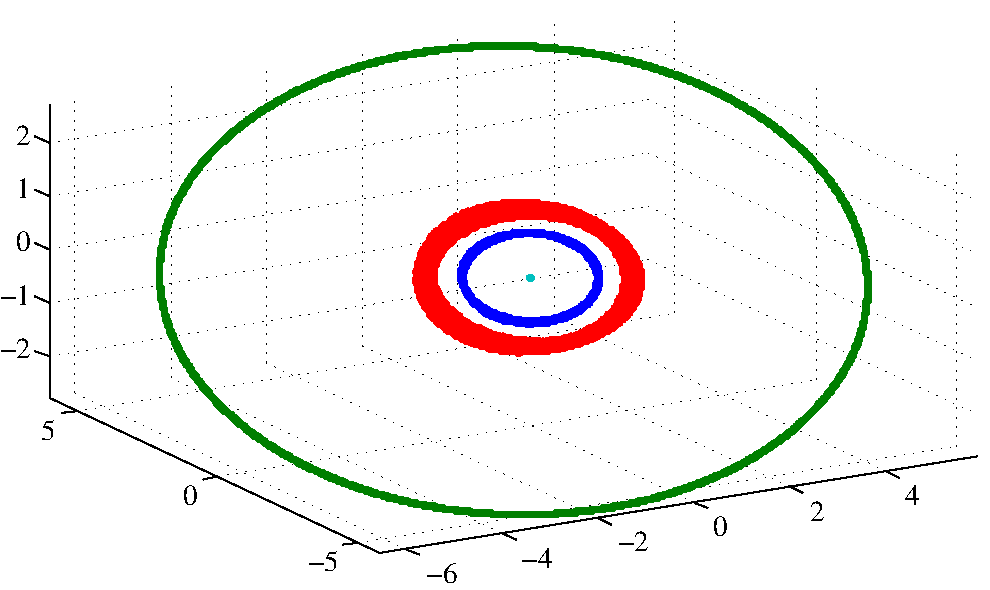
\includegraphics[width = 5.5in]{./figures/subSolSys}
  \caption[Sample Multi-body exosystem ]{ \label{fig:subSolSys} Orbits over 1 million years for exosystem composed of analogues of Earth (blue), Mars (red) and Jupiter (green), with a 1.5 $L_\odot$ star and orbits scaled such that all planets receive the same flux as they would in our solar system.  Note that over this time span, the Jupiter analogue causes significant deviations from the Keplerian approximation in the orbits of the two minor planets.  Scale units are in AU.}
\end{figure} 
While it is difficult to determine global stability of n-body systems, it is possible to determine local stability by integrating over long periods of time (millions of years) and searching for collisions or ejections (see \S\ref{sec:sysProp}).

The third approach to generating planetary systems represents the widest possible range of possible exosystems and is also the most difficult to apply.  One possibility is to `grow' solar systems by starting with simulated nebulae and utilizing a formation model to develop planets.  This is quite costly as it requires integrating many millions of years of the simulated system and often results in single-planet systems as bodies are ejected or destroyed.  An alternate method is to sample the known mass and semi-major axis distributions (see \reffig{fig:currHists}) and generate systems composed of multiple such bodies with initial conditions determined by Keplerian approximations.   However, using Keplerian approximations for initial conditions makes it difficult to simulate systems with non-Keplerian, n-body effects such as resonances \citep{fabrycky2010non} and long integrations are still required to ensure system stability.

The procedure for generating completely arbitrary planetary systems begins with the generation of $N$ random mass values according to the best-fit mass distribution.  From these masses the planetary radii are determined as follows:  For mass ranges up to 10$M_\oplus$, two random numbers are generated: a boolean value determining whether the planet will be a rock/iron or rock/ice mixture, and a random number uniformly distributed $\in [0,1]$, determining the fraction of rock via \refeq{eq:rockyPlanDensities}.  For giant planets, a uniformly distributed random number is generated in the range of [0,1] to represent the portion of mass in the planet's core, and radii values are interpolated from a lookup table based on values in \citet{fortney2007}.
 
Each planet is then associated with one of the target stars, with the likelihood of association given by the overall occurrence rate of planets and the iron abundance of the stars in the target list. Each planet is assigned an average albedo value ($p$) drawn from a uniform distribution in the range [$p_{min}$, $p_{max}$].  There is currently much work being done to model albedo values as functions of other planetary properties, but no one model is able to capture the entire parameter space \citep{sudarsky2005}.  For each planet, we generate initial positions and velocities by generating randomized average orbital elements via the distributions in \S\ref{sec:analytic_dists}. The mass of each target star is calculated from its absolute V magnitude ( $M_V$) via the relation:
\begin{equation}\label{eq:lmr}
\log(m_S/m_\odot) = 0.002456M_V^2 - 0.09711M_V + 0.4365 \,.
\end{equation}
 This relation has been shown empirically to be accurate to within 7\% for mass ranges corresponding to visual magnitudes between 1.45 and 10.25 \citep{henry1993}.  We treat the output of \refeq{eq:lmr} as the `estimated' mass and generate a `true' stellar mass as
\begin{equation}
m_S^{est} = m_S^{true}(1+ \nu)
\end{equation}
where $\nu$ is a random error term consistent with the known accuracy of \refeq{eq:lmr}.  The true masses are used for propagating the planets along their orbits, while the estimated masses of stars are needed for our return strategies, as described in \S\ref{sec:scheduling}.  This relation is used since it conveniently covers the range of visual magnitudes and stellar masses considered here.  However, newer mass-luminosity relations exist, with better accuracy for different mass ranges, and can be substituted for \refeq{eq:lmr} \citep{reid2002}.

At the end of this process, we have a target list encoded as an array of $N$ parameter sets
\begin{equation}\label{eq:simParamSet}
\{\begin{matrix} m_S^{est} &m_S^{true} & p_i & m_{P_i} & R_i & \mf r_{P_i/G} &  {}^\mc I \mf v_{P_i/G}& \mf r_{S/G} &  {}^\mc I \mf v_{S/G} \end{matrix} \}
\end{equation}
with $i = 1 \ldots n$ for a system of $n$ planets.  This parameter set can now be propagated forward in time to test the system stability and to perform mission simulations.  The set of parameter sets describing a group of simulated target systems will be referred to as a `universe' throughout the remainder of the text.

\subsection{System Propagation}\label{sec:sysProp}
Propagation of planets along their orbits can be done either by using the Keplerian formulation (which is exact only for a single-planet system) or by numerically integrating the Newtonian (\refeq{eq:nbody}) or post-Newtonian (\refeq{eq:einstein_nbody}) equations of motion.  If using the Keplerian formulation, the location of the planet is determined by the (possibly osculating) Keplerian elements and the current anomaly.  For the simulations in \S\ref{sec:case_studies}, the Keplerian propagation described here is used only for single-planet systems.  All simulations with multiple-planet systems use the n-body numerical integration methods described below.

From Equations (\ref{eq:Mdef}) and (\ref{eq:Pdef}) we can write:
\begin{equation}
M = \sqrt{\frac{\mu_S + \mu_P}{a^3}}(t - t_p) \, ,
\end{equation}
thereby directly relating the mean anomaly to the current time.  As the Kepler equation (\ref{eq:EtoM}) is non-invertible in $E$, we must use numerical methods in order to find the eccentric anomaly from the mean anomaly.  The simplest approach is to use Newton-Raphson iteration:
\begin{equation}\label{eq:NewtonRaphson}
E_{n+1} = E_n - \frac{M - E_n + e\sin E_n}{e\cos E_n - 1} \, .
\end{equation}
This iterant is applied to some initial value $E_0$ until convergence:
\begin{equation}
E_{n+1} - E_n < \varepsilon
\end{equation}
where $\varepsilon$ is typically set to the machine precision value of the data type being used \citep{moler2004numerical}.  This method produces excellent convergence as long as $E_0$ is sufficiently close to the true value for $E$.  For most values of eccentricity, it suffices to use $M$ for $E_0$, but in highly eccentric orbits, the mean and eccentric anomalies will differ greatly throughout the orbit.  An alternate approach to selecting $E_0$ lies in examining the Taylor expansion of the Kepler equation:
\begin{equation}
M = E - e\sin E \approx (1 - e)E + \frac{e E^3}{6} + \mc O(E^4) \,.
\end{equation}
We note that for a fixed value of $e$ and for $\vert M - E\vert >> \varepsilon$, one of the first two terms of the expansion is much larger than the other.  We therefore select $E_0$ as:
\begin{equation}\label{eq:E0selection}
E_0 = \left\{  
   \begin{array}{l l}
    \frac{M}{1 - e} & \frac{M}{1 - e} < \sqrt{\frac{6-6e}{e}}\\
   \left( \frac{6 M}{e} \right)^{\frac{1}{3}}& \mathrm{else}
    \end{array}
    \right.
\end{equation}
Because the Newton-Raphson algorithm is iterative, it is impossible to make it more time efficient than the minimum number of iterations required to achieve the desired precision.  However, using the initialization algorithm described above, machine double precision can be achieved for any eccentricity (up to $1 - \varepsilon$) in under 30 iterations for arbitrarily sized arrays of Mean anomalies and eccentricities (see \refcode{code:invKepler}).

While \refeq{eq:NewtonRaphson} is guaranteed to result in the correct anomalies for closed orbits, it starts with orbital elements, meaning that if planetary positions are recorded using a position and velocity state, it would be necessary to first apply Equations  (\ref{eq:vec2orbelem1}) - (\ref{eq:vec2orbelemf}) in order to find the osculating orbital elements.  Then, an updated mean anomaly would be defined as:
\begin{equation}
M(t) = \left(M(t_0) + 2\pi\frac{\Delta t}{P_{orb}}\right) \,\mathrm{mod}\,\, 2\pi \,,
\end{equation}
where $\Delta t$ is the desired time interval of the propagation ($\Delta t = t - t_0$) and mod represents the modulo operator.  \refeq{eq:NewtonRaphson} would then be applied to find E(t), from which the updated position and velocity could be calculated via Equations (\ref{eq:rpsrot}), (\ref{eq:rpsP1}), and (\ref{eq:vpsP1}).

A more direct method, which efficiently combines the conversion and iteration and is applicable to all orbits (open or closed), is described by \citet{shepperd1985universal}, based on work by  \citet{goodyear1965completely,goodyear1966general}.  Following \citet{sundman1913memoire}, the solution to \refeq{eq:twoBody} can be written as a function of a single parameter $w$ where:
\begin{equation}
\frac{\mathrm{d} t}{\mathrm{d} w} = \Vert \mf r_{P/S} \Vert \,.
\end{equation}
This solution (sometimes referred to as the `f and g method') allows us to update positions and velocities from their initial conditions:
\begin{equation}
\mf r_0 = \mf r_{P/S}(t_0) \quad \textrm{and} \quad \mf v_0 =  {}^\mc I \mf v_{P/S} (t_0)
\end{equation}
by using the algorithm:
\begin{align}
\upsilon_0 &= \mf r_0 \cdot \mf v_0  \,,\\
\beta &= \frac{2\mu}{\Vert \mf r_0\Vert} - \mf v_0 \cdot \mf v_0  \,,\\
r &= \Vert \mf r_0 \Vert U_0 + \upsilon_0 U_1 + (\mu_S + \mu_P) U_2  \,,\\
t &= \Vert \mf r_0 \Vert U_1 + \upsilon_0 U_2 + (\mu_S + \mu_P) U_3 \label{eq:altKeplerEq}  \,, \\
\mf r(t) &= f \mf r_0 + g \mf v_0 \label{eq:fandg}  \,,\\
\mf v(t) &= F \mf  r_0 + G \mf v_0 \label{eq:FandG}  \,,
\end{align}
where $U_n$ are the universal functions $U_n(w,\beta)$ \citep{battin1987introduction} and
\begin{equation}
\begin{array}{l c l >{\hspace{2cm}} l c l}
f &=& 1 - \frac{(\mu_S + \mu_P) U_2}{\Vert \mf r_0 \Vert} & g &=& \Vert \mf r_0 \Vert U_1 + \upsilon_0 U_2 \\
F &=& \frac{(\mu_S + \mu_P) U_1}{r \Vert \mf r_0 \Vert} & G &=& 1 - \frac{(\mu_S + \mu_P) U_2}{r} \,.
\end{array}
\end{equation}
The $f$ and $g$ functions may be equivalently defined in terms of the Keplerian orbital elements as:
\begin{equation}
\begin{split}
f &= 1 - \frac{\Vert \mf r \Vert}{\ell} + \frac{\Vert \mf r \Vert}{\ell}\cos(\nu - \nu_0) \,, \\
g &= \frac{\Vert \mf r \Vert \Vert \mf r_0 \Vert}{\sqrt{(\mu_S + \mu_P) \ell}}\sin(\nu - \nu_0)  \,,\\
F &= \sqrt{\frac{\mu_S + \mu_P}{\ell}}\tan\frac{\nu - \nu_0}{2}\left(\frac{1 - \cos(\nu - \nu_0)}{\ell} - \frac{1}{\Vert \mf r_0\Vert} - \frac{1}{\Vert \mf r \Vert} \right) \,, \\
G &= 1 - \frac{\Vert \mf r_0\Vert}{\Vert \mf r\Vert}\left(1 - \cos(\nu - \nu_0)\right) \,,
\end{split}
\end{equation}
where $\nu_0$ is the true anomaly at time $t_0$.

Note that $\beta$ is proportional to the orbital energy and \refeq{eq:altKeplerEq} is a reformulation of Kepler's equation in terms of $w$, which itself can be related to the eccentric anomaly as:
\begin{equation}
w = \frac{E - E_0}{\sqrt{\beta}} \,,
\end{equation}
where $E_0$ is the eccentric anomaly at $t_0$.

The universal functions $U_n(w,\beta)$ may be defined implicitly as:
\begin{align}
U_0 &= \left\{ \begin{array}{l l}
\cos(w\sqrt{\beta}) & \beta > 0\\
\cosh(w \sqrt{-\beta}) & \beta < 0 
\end{array}\right. \nonumber \\
U_1 &= \left\{ \begin{array}{l l}
\sin(w\sqrt{\beta})/\sqrt{\beta} & \beta > 0\\
\sinh(w \sqrt{-\beta})/\sqrt{-\beta} & \beta < 0 
\end{array}\right.  \\
U_{n+2} &= \frac{w^n}{\beta n!} - \frac{U_n}{\beta} \nonumber \,.
\end{align}
Unfortunately, this definition is not amenable to numerical implementation as the computation of the various trigonometric functions invariably introduces errors and often leads to singularities as various terms ($\beta$ especially) tend to zero.  The equivalent series representation:
\begin{equation}
U_n(w,\beta) = \sum_{k=0}^\infty \frac{(-\beta)^k w^{n+2k}}{(n+2k)!} \,
\end{equation}
is more tractable, but may still have convergence issues in the general case.  \citet{shepperd1985universal} solves this problem by introducing a change of variable:
\begin{equation}
u = \frac{U_1(w/4,\beta)}{U_0(w/4,\beta)} \,
\end{equation}
which falls strictly in the range $u \in [-\vert \beta \vert^{-\frac{1}{2}}, \vert \beta \vert^{-\frac{1}{2}}]$.  Since the alternate formulation of Kepler's equation in \refeq{eq:altKeplerEq} requires only the first few universal functions, the problem may be greatly simplified by writing:
\begin{align}
U_0\left(\frac{w}{2}, \beta\right) &= 1 - 2q \,, \\
U_0(w,\beta) &= 2U_0^2\left(\frac{w}{2},\beta\right) \,,\\
U_1\left(\frac{w}{2},\beta\right) &= 2(1-q)u\,, 
\end{align}
\begin{align}
U_1(w,\beta) &= 2U_0\left(\frac{w}{2},\beta\right)U_1\left(\frac{w}{2},\beta\right) \,, \\
U_2(w,\beta) &= 2U_1^2\left(\frac{w}{2},\beta\right) \,,
\end{align}
where
\begin{equation}
q = \frac{\beta u^2}{1 + \beta u^2} \,.
\end{equation}
Furthermore, 
\begin{equation}
U_3(w,\beta) = \frac{4}{3} U_1^3\left(\frac{w}{2},\beta\right) G(3,0,\frac{3}{2},q) \,,
\end{equation}
where $G$ is the continued fraction expansion of the ratio of the ratio of two hypergeometric series:
\begin{equation}
G(a,b;c;z) = \frac{{}_2F_1(a,b+1;c+1;z)}{{}_2F_1(a,b;c;z)} \,,
\end{equation}
with the Gaussian hypergeometric function defined as in \refeq{eq:gaussHyper}.

Returning to Equations (\ref{eq:fandg}) and (\ref{eq:FandG}), we see that the position and velocity can be updated via a simple matrix multiplication:
\begin{equation}
\left[\begin{matrix} \mf r(t) \\ \mf v(t) \end{matrix} \right] = \left[\begin{matrix} f I_3 & g I_3 \\ F I_3 & G I_3\end{matrix} \right]\left[\begin{matrix} \mf r_0 \\  \mf v_0 \end{matrix} \right] \,,
\end{equation}
where $I_3$ represents the $3\times3$ identity matrix.  Multiple bodies can be updated together by making the state transition matrix block diagonal and stacking positions and velocities into a single column vector:
\begin{equation}\label{eq:stackedState}
\left[\begin{matrix} \mf r_1(t) \\ \mf v_1(t) \\ \vdots \\   \mf r_n(t) \\ \mf v_n(t)\end{matrix} \right] =
\left[\begin{matrix} 
\left[\begin{matrix}f_1 I_3 & g_1 I_3 \\ 
F_1 I_3 & G_1 I_3\end{matrix} \right] & &\\
&  \ddots &  \\
& &\left[\begin{matrix} f_n I_3 & g_n I_3   \\ 
F_n I_3 & G_n I_3 \end{matrix} \right]
\end{matrix} \right]\left[\begin{matrix}  \mf r_1(t_0) \\ \mf v_1(t_0) \\ \vdots \\   \mf r_n(t_0) \\ \mf v_n(t_0)\end{matrix} \right] \,.
\end{equation}

In this formulation, the Kepler equation is solved via Newton-Raphson iteration on the independent variable, $u$:
\begin{equation}
u_{n+1} = u_n - \frac{t - \Delta t}{4(1 - q) r} \,.
\end{equation}
A secondary iteration is required to evaluate the function $G$.  A convenient algorithm is Shepperd's modification of Gautschi's method for the evaluation of continued fractions.  To evaluate the function $G(a,b;c;z)$, a set of intermediate variables is initialized as:
\begin{align}
k_0 &= 1 - 2(a - b) \,,\\
l_0 &= 2(c-1) \,, \\
d_0 &= 4c(c-1) \,, \\
m_0 &= 4b(c-a) \,, \\
A_0 &= B_0 = G_0 = 1 \,,
\end{align} 
and then iterated until convergence via:
\begin{align}
k_{n+1} &= -k_n \,,\\
l_{n+1} &= l_n + 2 \,, \\
d_{n+1} &= d_n + 4l_{n+1} \,, \\
m_{n+1} &= m_n + (1+k_{n+1})l_{n+1} \,, 
\\
A_{n+1} &= \frac{d_{n+1}}{d_{n+1} - m_{n+1} A_n z} \,,\\
B_{n+1} &= (A_{n+1} - 1)B_n \,,\\
G_{n+1} &= G_n + B_{n+1} \,.
\end{align} 
An implementation of the full algorithm is shown in \refcode{code:keplerSTM}.

For multi-planet system, we abandon the Keplerian propagation in favor of numerical integration of \refeq{eq:nbody}.  While this is more computationally intensive, it produces much more accurate results in systems with multiple planets, especially when one or more of these is Jupiter-size or larger.  More importantly, the Keplerian formulation cannot be used to generate consistent stellar reflexes in multi-planet system and is therefore a poor model for studying precision astrometry and radial velocity.  Because the Keplerian formulation places the star at the  origin of a frame that is treated as inertial, the Keplerian formalism implies that the star does not move.  Using the standard definition for center of mass, $G$,:
\begin{equation}
\sum_{k\in X}m_k \mf r_k/G = 0 \,,
\end{equation}
where $X$ is the set of all of the bodies in the exosystem (see \refeq{eq:Xsetdef}), the position of the star with respect to the barycenter is:
\begin{equation}\label{eq:keplerCOM}
\mf r_{S/G} = -\frac{\sum_{k \in Y} m_k \mf r_{k/S}}{\sum_{j \in X} m_j} \,,
\end{equation}
where $Y$ is now the set of all exosystem bodies excluding the star, $Y = X\backslash \{S\}$.  
If we consider the Newtonian formulation of the two body problem, as in \refeq{eq:twoBody}, with 
\begin{equation}
\mf r_{P/S} = \mf r_{P/G} - \mf r_{S/G} \,,
\end{equation}
where $G$ is now the barycenter of the two-body system, we see that \refeq{eq:keplerCOM} is the average of the star position with respect to the barycenter of each of the two-body systems composed of the star and each individual planet.  This means that rather than modeling the true interactions of all of the bodies in the system, the best that can be accomplished via the Keplerian model is a first order approximation of the true stellar motions.

The specific method used for the numerical integration is very important.  Because an orbital system with no external perturbations is a canonical Hamiltonian system, it is important to ensure that energy is being conserved.  Low order Runge-Kutta methods will not do so, deviating quite quickly from the true system state.  The solution is to use either high order integrators, or one of a class  of symplectic integration schemes.  Of particular interest are the Runge-Kutta-Nystr\"{o}m (RKN) methods as they are specifically formulated to solve second order ODEs that are cyclic in the first derivative of the state:
\begin{equation}
\frac{d^2}{dt^2} y = f(y) \,.
\end{equation}
While these methods also do not guarantee that energy will be preserved, they are canonical, and sufficiently high-order implementations preserve energy to a very large degree \citep{qin1991}.  \reffig{fig:integratorComp} shows a comparison of energy variation over time in numerical integrations of the solar system.
\begin{figure}[ht]
 \center
 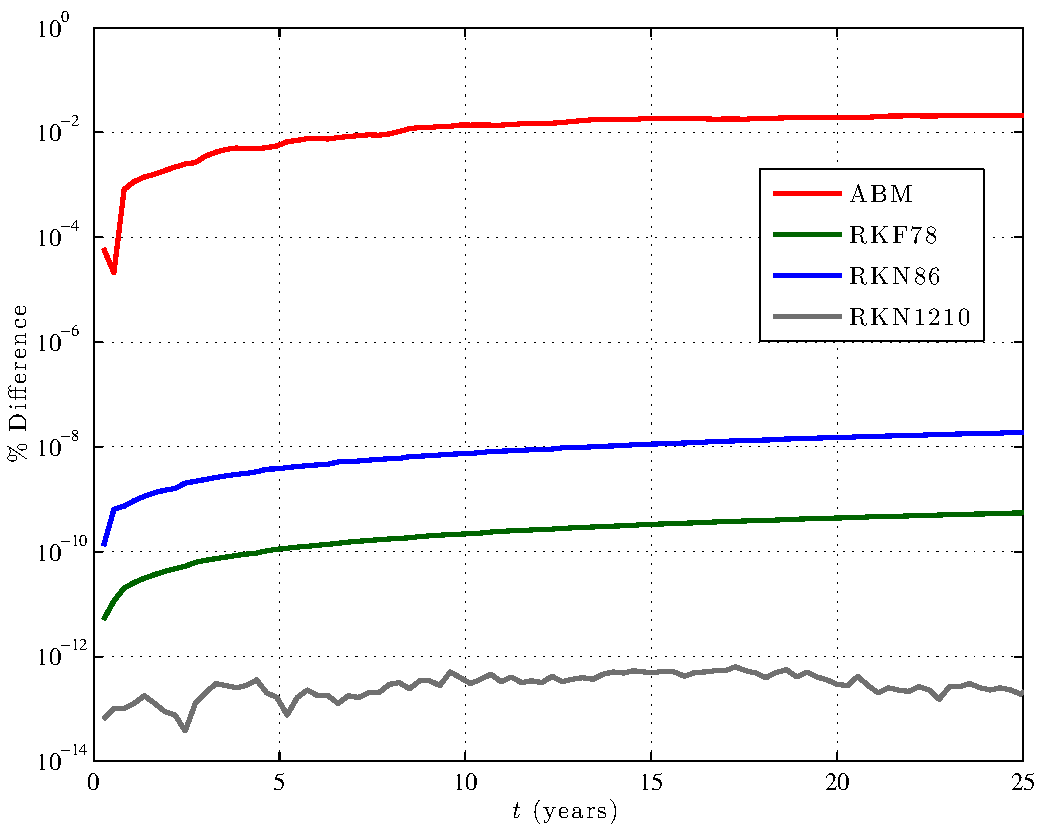
\includegraphics[width= 5.5in]{./figures/integratorComp}
  \caption[Integrator Comparison]{ \label{fig:integratorComp} Change in total energy (\refeq{eq:Etot} over 25 years of integration of the solar system using different numerical solvers with identical initial conditions.}
\end{figure} 
Unlike the two RKN implementations, the Adams-Bashforth-Moulton (ABM) PECE (prediction-evaluation-correction-evaluation) multi-step solver \citep{shampine1975computer} and Runge-Kutta-Fehlberg (RKF) 7(8) solver \citep{fehlberg1968classical}, operate on first order ODEs.  However, the high order of the Runge-Kutta-Fehlberg (RKF) makes it outperform the (relatively) lower-order Runge-Kutta-Nystr\"{o}m 8(6) solver \citep{papakostas2000,qin1991} in terms of energy conservation.  The overall best performance is achieved with the  Runge-Kutta-Nystr\"{o}m 12(10) solver \citep{dormand1987high}.  The ABM solver, while multistep, does not have volume or energy preserving qualities and is thus the poorest  choice.  Over relatively short periods (less than 1 million years), the 12/10th order RKN solver is energy-preserving to within machine double precision.  For most system energy is stable on the order of $10^{-12}\%$ over billions of years. 

It is also common to use hybrid-symplectic integrators which use symplectic integration schemes when masses interact closely, and non-symplectic schemes the rest of the time to greatly increase the speed of integration without losing the energy-conserving properties of fully symplectic integrators \citep{chambers1999hybrid}.  However, because of the amenability of the n-body equation to vectorization, and the constantly increasing speed of computer processors, very high-order methods such as the RKN 12(10) solver can be run with integration times of billions of years in feasible amounts of computer time by using variable time steps and efficient error estimation algorithms \citep{tsitouras1999cheap}.  \refeq{eq:nbody} can be evaluated very efficiently by precomputing four indexing arrays.  For a state vector $x$ representing $n$ bodies, with positions and velocities stacked in a column vector as in \refeq{eq:stackedState}, $[j]$ is a vector of $9n$ elements filled with indices from $1$ to $n$ each repeated $n-1$ times:
\begin{equation}
[j] = [1, 1, \ldots , 1, 2, 2, \ldots , 2, \ldots , n] \,.
\end{equation}
The vector $[k]$ also has $9n$ elements, but is filled by circularly permuting the indices such that $k \ne j$:
\begin{equation}
[j] = [2,3, \ldots , n, 1, 3, \ldots , n, 1, 2, 3,\ldots , n,\ldots ,1,\ldots ,n-1] \,.
\end{equation}
Finally, two indexing matrices are required: [z1] contains indices $1\ldots3n$, arranged in a matrix of dimension $3 \times n$ and [z2] contains indices $1\ldots n(n-1)$, arranged in a matrix of dimension $n \times n-1$.  In this way, every required combination of position differences can be computed as by indexing the state with $[z1]$ recursively indexed by $[j]$ and $[k]$ and \refeq{eq:nbody} can be evaluated by summing over the columns of the matrix resulting from indexing the difference combinations with $[z2]$.  An implementation of this algorithm is presented in \refcode{code:nbodyVect}.

Numerical integration also makes it simple to search for specific events, such as collisions (when $\Vert \mf r_{k/j} \Vert < R_k + R_j$) or ejections (when specific orbital energy changes sign).  The basic approach is to define a set of continuous functions that cross zero when an event of interest occurs and then to use root finding methods such as Regula-Falsi to pinpoint the exact time of the event when a sign change occurs in the function evaluation between integrator iterations \citep{press1992numerical}.  In this fashion the stability of generated exosystems can be evaluated by simply integrating for a period of one million years or more (depending on the time spans predicted by the planetary formation and evolution theories used).

\section{Target Selection and Availability}\label{sec:targ_selection}
A major factor in the planning and outcome of any planet-finding mission is the fact that we are limited to a very specific, non-isotropic population of possible target stars.  Each detection method has limitations on what stars can be used, and a specific preferred type of star, limiting which stars can be added to the target pool.  For example, for direct imaging of Earth-like planets, we need nearby stars so that we can observe large portions of their habitable zones.  We would also like to have low exo-zodi contributions, making older stars preferential, and would likely concentrate on F, G, and K stars similar to the sun.  On the other hand, if we were looking for self-luminous giant planets, we would preferentially target young systems with hot A and B stars.  Instrument characteristics and mission goals will always drive the initial pool of stars, but the final target list has an equally dramatic effect on the mission science returns.

For direct imaging, we always start with a list of all of the stars about which a planet from the planetary population of interest  could, at some point in its orbit, be observable by our instrument.  For example, if we are interested in Earth-twins in the habitable zone, we leave only those stars where a randomly oriented habitable zone orbit leaves the planet outside the instrument's projected IWA for a time longer than the required detection integration time for that star (as defined in \S\ref{sec:model_obs}).  In order to decide whether a given star can have detectable planets in a region of interest (defined by some range of $a$ and $e$), we need to find the smallest possible $\Delta$mag for a planet in this region that corresponds to a value of $s$ greater than the projected IWA.  This is done as follows:
\begin{enumerate}
\item Find $\beta^\star$ that minimizes $\Phi(\beta)\sin^2(\beta)$.
\item Define the range of orbital distances as $r = [a_{min}(1-e_{max}),a_{max}(1+e_{max})]$.
\item Define $s_{\beta^\star} = r\sin\beta^\star$ and $\hat{r} = \textrm{IWA}*d/\sqrt{L} \sin\beta^\star$ - the minimum $r$ such that $s_{\beta^\star} >  \textrm{IWA}*d/\sqrt{L} $.
\item If $\hat{r} \in r$ then $s =  \textrm{IWA}*d/\sqrt{L}$ and $\beta = \beta^\star$.
\item If $\hat{r} < r$ then $s = \min(r)$ and $\beta = \beta^\star$.
\item if $\hat{r} > r$ then $s =  \textrm{IWA}*d/\sqrt{L}$ and $\beta = \sin(\textrm{IWA}*d/\sqrt{L}/\max(r))$.
\end{enumerate}
The $s$ and $\beta$ values produced by this algorithm represent the minimum value of $\Delta$mag for any planet in the region of interest, with the corresponding $s$ value outside the projected IWA.  If this $\Delta$mag value falls below the limit of the instrument's photometric sensitivity, then the star is considered a candidate. 

Additional criteria for the target list may include:
\begin{itemize}
\item Stars on the main sequence
\item Stars with high life expectancy (B-V Johnson magnitude > 0.3)
\item No low metallicity stars (higher probability of planets, see \reffig{fig:marcyFEH} 
\item No stars with high intrinsic variability (to remove major photometric variations)
\item No binaries or stars with close companions or nearby bright background stars (since most starlight suppression systems cannot work on multiple sources)
\item Maximum apparent magnitude (brighter stars only)
\item No young stars (so that planets will have formed)
\end{itemize}
 Young stars may be identified by X-ray emission for stars more distant than 15 pc (detected by ROSAT) \citep{guillout1999stellar}, by chromospheric variability, by rotational periods of less than 10 days, or projected rotational velocity of greater than 5 km/s. For a typical imaging mission such as the ones in \S\ref{sec:case_studies}, we start with the 1612 non-binary stars within 30 pc of our solar system.  For an IWA of 75 mas and $\Delta$mag$_0$ of 26, applying the procedure above to the subset of main sequence stars yields 372 possible target stars.  With those instrument specifications, 144 of these targets have single-visit completeness values of less than 0.01, and 260 have completeness values of less than 0.1.

The biggest problem in selecting the target list comes from one of the inherent trade-offs in the stated science goals.  The desire to visit as many unique targets as possible means that the overall probability of detecting planets is decreased by including lower completeness stars (where the probability of detection is smaller).  On the other hand,  only visiting a small number of stars automatically limits the number of unique detections that can be made, and if the frequency of the planet type you are searching for (or absolute frequency of all planets) happens to be low, having a large target pool may be the only way to detect any planets at all.  An additional problem lies in trying to filter target stars by the amount of integration time required.  Although we can calculate the integration time for any assumed $\Delta$mag value, in reality, planets from any population of interest can vary by several magnitudes at the time of observation.  For example, an Earth-twin observed at one point on its (habitable zone) orbit at a $\Delta$mag of 26 will require 200 days for spectral characterization.  The same planet, at a different orbital position can have a $\Delta$mag of 25, which would require only 30 days of integration.  In both cases, the time required to determine whether a detection has occurred is less than 2 days.  Because of the great disparity in detection and characterization times, and since high ecliptic latitude stars have very long observing seasons, improper mission simulation logic can sometimes lead to extremely long integration times which adversely affect overall mission performance.

Because we cannot assume \emph{a priori} knowledge of  planet frequency, or what the brightness of planets will be at the moment of detection, it is quite difficult to address these issues using scheduling logic alone.  Instead, we can introduce two additional parameters: a minimum target system completeness value, and a maximum single integration time.  The minimum completeness gives us a systematic way to limit the size of target lists, mapping directly to the unique targets vs.~total detections tradeoff. The maximum integration time allows us to include all potential targets, but not allow any one integration to significantly affect the mission outcome.  This value can be used in two different ways: first, the target list is filtered so that no detection time for the worst case (highest zodi level and limiting $\Delta$mag) exceeds the minimum integration time.  Second, in visits where a detection occurs, but the spectral characterization would take more than the maximum integration time, the spectral characterization is not attempted. 

The proper value for each of these parameters is found by performing a line search over multiple simulations with these values smoothly varied to optimize specific target metrics.  For all of the instruments and mission scenarios evaluated to date, there is improvement in the number of total and unique detections when the minimum completeness is raised from zero.  Specific improvements vary between instrument and spacecraft designs, but all systems perform better with a minimum completeness of 0.1, as opposed to using the full target list.  In cases where low completeness stars (completeness  $< 0.1$) do provide detections, these are always very dim, require much longer integration times to acquire a spectrum, and are never detected again.  The integration time cutoff is harder to optimize due to the larger search space and the computational costs associated with running many simulations.  In certain cases, the instrument design itself leads to a systematic limit on the length of observations, thereby automatically providing a maximum integration time.  In other cases, good results were achieved by setting the maximum integration time based on the total observation time available and the average time to transfer between targets.

For ground based observatories, target availability is given strictly by the observatory location and the time of year.  Space telescopes, however, can reside in a variety of orbits, and target availability may differ greatly from one observation to the next.  Missions such as Kepler, whose target pool is always in the field of view do not have any scheduling considerations associated with target availability, so the discussion in this section is limited to direct imaging missions and hybrid missions with targeted transit photometry or other planet-finding observations.

In general, whether a target star is observable at a specific point in time can be determined by calculating the angle between the telescope-sun and telescope-target vectors:
\begin{equation}
\theta = \cos^{-1}\left(\hat{\mf r}_{S/sc} \cdot \hat{\mf r}_{S_0/sc}\right)
\end{equation}
where $S_0$ refers to our sun.  For any given telescope, the sun cannot be within some number of degrees of the line of sight ($\hat{\mf r}_{S/sc}$ - the spacecraft-target vector) or light from the sun would enter the telescope aperture.  For a  telescope with a completely unshielded primary, this value would be nearly 180$^\circ$.  However, most optical telescopes are designed with the primary enclosed within the spacecraft and many proposed designs (especially for direct imaging) have sun shields that further extend the permissible location of the sun.  With these additions, the sun exclusion (or `keep-out') zone can be as low as 45$^\circ$.

\begin{figure}[ht]
 \center
 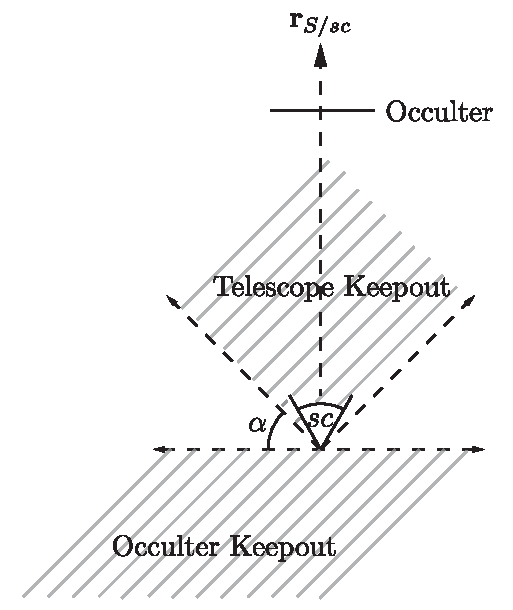
\includegraphics[width=2.75in]{./figures/keepoutZones}
  \caption[keep-out Zones]{ \label{fig:keep-outZones} Schematic top-view of telescope and occulter spacecraft and associated keep-out zones.  An observation can only be made when the sun (and any other sufficiently bright bodies such as the Earth or moon) is in the annulus extending $\alpha$ degrees (the complement to the sun-exclusion telescope angle) from the line orthogonal to $\mf r_{S/sc}$ at the telescope aperture.  If there is no external occulter, then the annulus also includes the 180$^\circ$ below this line.}
\end{figure} 

If the optical system is self contained, the sun exclusion angle is the only factor determining whether a star is in the keep-out zone.  Unfortunately, systems with external optical elements, such as free-flying occulters, have an additional keep-out zone so that sunlight isn't reflected by the external elements into the telescope.  Because of the nature of these systems, this keep-out region must cover the full 180$^\circ$ region below the line orthogonal to the line of sight (see \reffig{fig:keep-outZones}). It is possible to reduce this keep-out by tilting the occulter, at the expense of requiring larger starshades (as the effective shadow region is diminished) \citep{brown2010new}.


\section{Decision Modeling}\label{sec:scheduling}

While the assumptions and definitions in \S\ref{sec:model_obs} are sufficient to model any single observation with an imaging instrument, they are not enough to automatically generate an entire mission (or survey) timeline.  This is primarily due to the limitation of imaging systems to only one target at a time, and the strong stochastic element in the outcome of any one observation.  The amount of time spent on any one target will depend on whether an observable planet exists there, and also on how mission rules dictate that time be allocated to spectral characterization versus finding new planets.  Because the length of every observation is variable, the subset of available targets for the next observation (see \S\ref{sec:targ_selection}) will be constantly changing, and it is thus impossible to assemble an exact observation schedule before the start of operations.  For ground-based observatories, there is a natural cadence imposed by the day-night cycle, but it is still possible to optimize operations during a single night of observing, if real-time processing is employed.  Our goal is to develop a scheduling algorithm that will be able to make decisions based on the time history of previous observations.

Our automatic scheduler is defined as an optimization problem wherein we seek to maximize the science yield of a mission by simultaneously maximizing the number of unique planets discovered, the number of spectral characterizations of discovered planets, the number of planets observed enough times to produce orbital fits, and the portion of the target list observed at least once.  This last goal is included since there is scientific merit in any observation, whether or not a planet is detected (in the form of disk science and concurrent observations by other instruments on the observatory), and this provides a simple way of controlling the decision algorithm's natural bias towards higher completeness stars.  It must be noted that several of these science tasks are inherently antithetical---for example, spending time on finding more unique planets means less time devoted to scheduling additional observations for previously found planets, and thus fewer orbital fits.  This conflict is addressed by introducing weights to our cost function, which can be used to tune the relative importance of each science goal.

 Previous implementations of automated planning have modeled the order of observations as a traveling salesman problem (TSP) with repeated visits---a useful model as there exists a large body of work on methods for solving it \citep{kolemen2007}. Unfortunately, it is difficult to create a realistic mission simulation with this approach.  Unlike the classical TSP, where path lengths between locations are fixed and the group of locations remains invariant, here, the cost of transferring between a pair of target stars is time dependent, and the amount of time required at each target is variable, and cannot be known \emph{a priori}.  For these reasons, even the time-dependent TSP description of the system is inadequate.

Instead, as with a TSP, we represent the sequence of visits as a directed graph with variable length edges.  The graph is encoded as an $N \times N$ matrix (for $N$ targets), where element $ij$ represents the `cost' associated with switching from target $i$ to target $j$ (which we shall refer to as `transiting' between targets).  We can use a variety of graph search techniques to determine the optimum (least cost) path, by assuming that this matrix will remain constant for $k$ transits (where $k$ is determined by the specifics of the system being simulated), and thus pick the next target as the node generating the least cost path.  After a target is observed, however, the entire matrix is re-generated based on the current location of the spacecraft, and the process is repeated, thereby capturing the dynamic nature of the problem.  We can also take the approach of simply always going to the `best' (lowest cost) available target, by setting $k = 1$.  In cases where the matrix is relatively stable over multiple steps (i.e., the time spent on each target is small), the re-evaluation of the costs does not produce significant changes in the planned path.  However, in those cases where one observation takes a long time (i.e., when spectral characterization is required), the costs will change significantly, so it is very important to update the matrix to select the next best target.

The function determining the cost of each transit is a weighted linear combination of multiple factors,
\begin{equation}\label{eq:costfunc}
\begin{split}
A_{ij}  &= \left[ a_1 \frac{\cos^{-1}\left(u_i \cdot u_j\right)}{2\pi}B_{inst} + a_2 \textrm{comp}_j  \right. \\ 
&{} - a_3 e^{t_c-t_f} B_{unvisited} +  a_4 B_{visited}(1-B_{revisit})\\
&\left.{}  - a_5 B_{revisit} \left(\frac{N_j}{N_{req}} \right)(N_j < N_{req}) - a_6 \frac{\tau_j}{\textrm{vis}_j} \right] /(1-B_{keep-out}) \, .
\end{split}
\end{equation}
The first term represents the cost associated with retargeting, with $B_{inst}$ set equal to 0 for ground-based telescopes and space coronagraphs (since the amount of fuel and time used in retargeting should be approximately constant for an internal coronagraph for any pair of targets). $B_{inst}$ is set to 1 for space telescopes with external occulters, or any other system where a spacecraft needs to be physically repositioned in the line of sight from telescope to target.  While this term is not the actual cost associated with each specific retargeting (which depends on the position of the spacecraft and its orbit), it serves as a good heuristic function.  Because the orbits assumed for the telescope and occulter typically require active control to retarget in a reasonable amount of time, and the contribution of the orbital dynamics to the time and fuel costs of retargeting are comparatively small, in most cases this represents an admissible heuristic, and produces good results \citep{kolemen2007}. 

In calculating the actual transit time and fuel used, the full orbital dynamics and spacecraft masses are taken into account, and the masses are updated after each transit to reflect fuel use.  Following \citet{kolemen2008thesis}, transits are modeled either as impulsive thrusts or continuous point-to-point trajectories.  In each case, the aim is to find an occulter trajectory such that the telescope-occulter separation is fixed at the end, with inertial velocities matched. In the impulsive case, this is achieved with two large maneuvers at the beginning and end of the trajectory which are taken to change the occulter's velocity while keeping its position nearly constant.  This becomes a boundary value problem with the 3 dimensional velocity vectors at the trajectory endpoints as the unknowns, which can be solved via collocation.  

In the case where longer thrust times are required (such as with electric propulsion), the strategy is to minimize the control effort given the differential equations of motion and fixed endpoints (a fixed transfer time is assumed), which results in a 12 dimensional boundary value problem.  A detailed treatment of this problem type can be found in  \citet{stengel1994optimal} and the particular problem is analyzed in \citet{kolemen2007,kolemen2008thesis}.  Fuel use is calculated by assuming that the spacecraft mass is nearly constant during any impulsive thrust maneuver and taking the product of the burn time with the propulsion system mass flow rate, which is determined by the system  $I_{sp}\addsymbol{$I_{sp}$}{Specific Impulse}$ and thrust force.

The first term (when $B_{inst}$ is not zero) can be efficiently constructed by first generating a matrix of all of the combinations of the currently available target pool taken two at a time:
\begin{equation}
[c] = \left[ \binom{N_t}{2} \right] \,
\end{equation}
where $N_t$ is the size of the currently available target pool.  A vector of angular separations is calculated as in \refeq{eq:costfunc}:
\begin{equation}
[a] = \frac{\cos^{-1}\left(u_i \cdot u_j\right)}{2\pi}
\end{equation}
and then indexed via a strictly upper triangular (zero diagonal) matrix of ones to generate an upper triangular matrix of angular distances.  The result of this operation, when added to its transpose, generates the required matrix of the first term.  A sample implementation is presented in \refcode{code:genCostFunTerm1}.

For occulters designed to operate at multiple separation distances the slews required in order to complete spectral characterizations introduce high costs in terms of both fuel and time.  It is important to remember, however, that there is no effective way of minimizing these costs other than by changing the occulter design, so they need not be included in the transition cost function.  Since covering the whole spectral band is usually a mission requirement and observing seasons for most stars are relatively short, we have no choice but to move the occulter in at full thrust if characterizing the whole spectral band is to be attempted during a single visit.  Thus, the fuel/time cost of this extra slew is essentially constant (changing only gradually with the decreasing spacecraft mass) and does not affect the transition cost calculation any more than spectral characterizations performed by a coronagraph.  The only changes this system requires in the simulation logic are as follows: The occulter is moved for spectral characterization only if the star will remain observable for enough time to perform the slew and the second spectral integration.  In cases where the first half of the spectrum is acquired, but not the second, on revisits the occulter is slewed directly to the closer separation distance.  Because the smooth trajectories between the two separation positions do not take significantly different amounts of time or fuel, the heuristic term in the original cost function still applies.

The second term of the cost function serves as a heuristic for the probability of a detection at the next target, with  $\textrm{comp}_j$ equal to one minus the completeness of the $j$th target.  The third term is included to promote visits to as many unique targets as possible.  Here,  $t_c$ is the current time, $t_f$ is the mission lifetime, and $B_{unvisited}$ is a boolean equal to 1 if target $j$ has not been visited.  The fourth term creates a preference for targets that are scheduled for a revisit, with boolean $B_{visited}$  set to 1 if target $j$ has been visited, and boolean $B_{revisit}$ set to 1 if target $j$ is currently scheduled for a revisit (`currently', in this case, means $\pm$ the average re-targeting time).  The fifth term is included to improve the odds of good orbital fits.  $N_j$ is the number of previous detections of a planet at target $j$, and $N_{req}$ is the number of detections required for an orbital fit.  This term has the effect of biasing target selection towards those stars with more prior detections as they near the minimum required number of detections, when they are scheduled for revisits.  The inequality expression represents a boolean that eliminates the effect of this term once the required number of detections has been achieved.  

Nominally, we set $N_{req}$ to be four, but depending on the system and desired accuracy of derived orbital elements, many more detections may be required.  Since the method used to schedule future observations depends on an estimate of the semi-major axis, which is updated with each subsequent observation, we have found that four detections are generally enough to constrain the semi-major axes of planets in the limited population considered here to below 10\% error (in some cases to within 1\%).  Four visits also constrain the possible ranges of the other orbital parameters, giving us the ability to say with high confidence whether the planet is in the habitable zone.  Nevertheless, previous work has shown that orbital fitting accurate enough to predict the future positions of planets is very difficult, and may require many more observations, especially when considering more diverse populations of planets \citep{pravdo2007observation, brown2007minimumTPF}. 

The final term inside the brackets was included after a study of strategies employed in the manual scheduling of planet finding missions.  The most valuable of these strategies is to identify the stars closest to `leaving' a keep-out zone, and thus provide the maximum amount of possible integration time for the instrument.  This strategy has the additional benefit of creating a schedule in which an occulter does not need to move from target to target at full thrust (since slew times are determined by how much time is left until the star is viewable), thus saving large amounts of fuel.  This strategy is achieved by the sixth term, where $\tau_j$ is the amount of time before star $j$ enters a viewable zone (this value is negative if the star is already outside of the keep-out zone) and $\textrm{vis}_j$ is the total amount of time star $j$ is continuously viewable. This term has the effect of making stars about to enter a viewable portion of the sky more likely to be selected, while penalizing those that are about to enter a keep-out zone. 

The factors $a_i$ are selected to weight the relative importance of the various terms in \refeq{eq:costfunc}.  For the validation results presented in the next section, these terms were chosen manually, after experimenting with varying values.  Obviously, these weights represent a great opportunity for optimization and possibly auto-tuning during the course of a single simulation.  However, even with only six parameters, the search space of possible values is quite large, making an optimization remarkably computationally intensive.  The weights are also fairly specific to individual instrument designs, meaning that they cannot be carried over to new configurations unless these are fairly similar to previously analyzed ones.  Limited optimization, in the form of an unconstrained simplex search \citep{lagarias1999convergence} over a scalar cost function was carried out for the designs in \S\ref{sec:case_studies}.

Finally, $B_{keep-out}$ is a boolean representing whether a given star is currently in the keep-out zone.  Dividing by 1 minus this term leads to infinite costs for stars currently in the keep-out, so they are never selected; the same is done for the matrix diagonal so that the same target is not visited twice in a row.  For an occulter system, stars are only considered to be in the keep-out zone if they will be unobservable when the occulter completes its transition slew.  That is, if the amount of time until they become viewable would result in a transit slew using less than some selected factor of the slew time for thrusting (typically, we use 50\%), or if they could not be reached at full thrust before entering the keep-out zone.  Another way of controlling this is to define a default burn portion---that is, the default portion of the transfer maneuver that is used for accelerating and decelerating (with the remainder used for coasting).  This allows for an initial estimate of the slew times required to get to the next set of targets.  After the next target is selected, the actual burn portion used can be adjusted as necessary to achieve the desired transfer time.  Decreasing this parameter has the effect of saving fuel, as fuel use increases roughly as the square of the acceleration time, while potentially decreasing the number of targets visited. \reffig{fig:adjmat} shows a graphical representation of a cost function matrix.  In this case, all targets are included, leading to many whole columns of infinite values (for stars in the keep-out zone), however, to improve the efficiency of the simulation costs may be calculated only for the subset of stars not in the keep-out zone.
\begin{figure}[ht]
\centering
   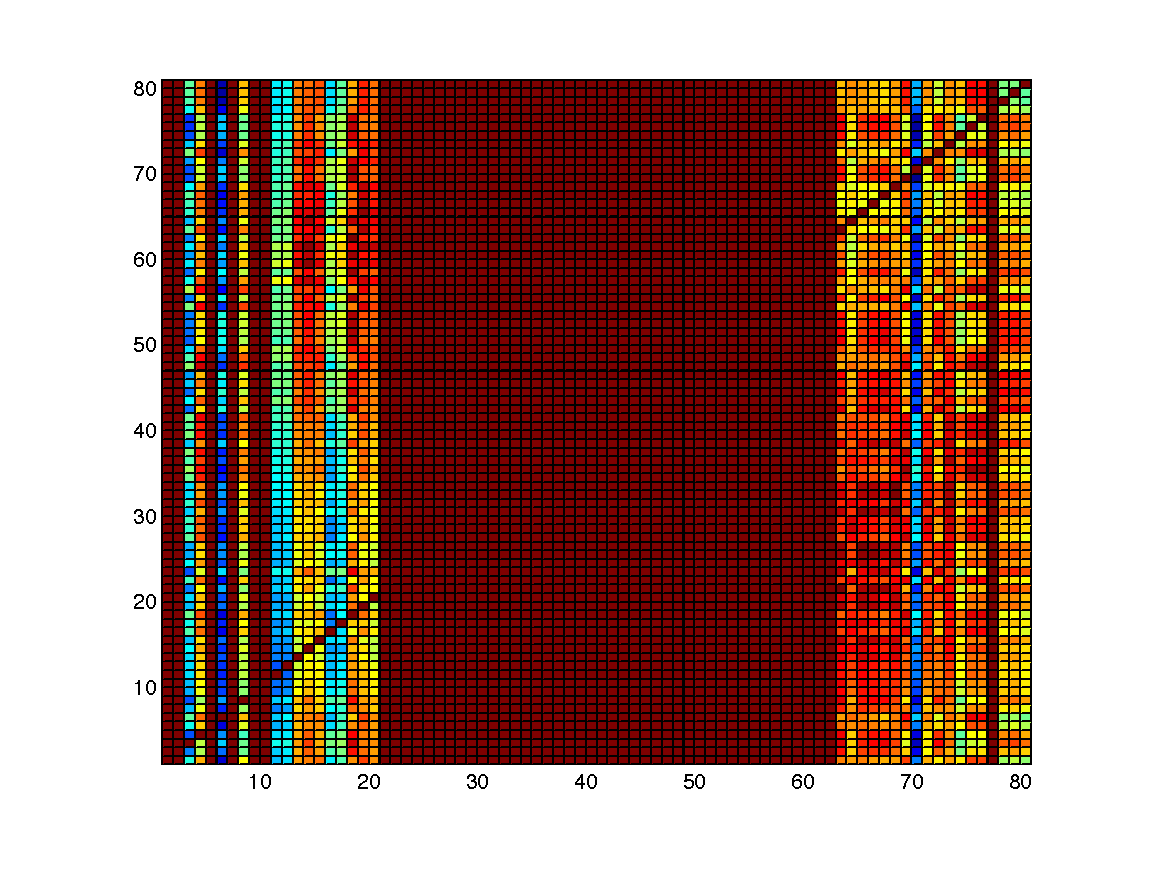
\includegraphics[width = 5.5in,clip=true,trim=0.5in 0.3in 0.5in 0.3in]{./figures/adjmatfig}
 \caption[Cost Function Matrix]{ \label{fig:adjmat} Visualization of cost function matrix.  All stars (including those in the keep-out zone) were included, leading to multiple columns of inifinite cost. The transition cost increases from blue to red.}
 \end{figure}

For the instruments considered in \S\ref{sec:case_studies}, those with an occulter will have transfer times between targets on the order of weeks, so that $k$ must be quite small---just two or three steps.  This makes it easy to compute all possible path costs and take the one representing the true minimum.  Self-contained coronagraphs, on the other hand, can acquire a new target in as little as a single day, while ground-based systems can retarget in just minutes, so that it is possible to use a much larger $k$, which would require switching to a different selection method (such as an iterative deepening search).  However, simulation shows that due to the relatively small target pools available, in most cases, just using the first 3 to 5 steps produces the same result as a more exhaustive search.  To minimize computing time fixed $k$ values of 3 are used for these instruments, except when directly testing the effects of varying this parameter.

The list of scheduled revisits (used to set the $B_{revisit}$ term in \refeq{eq:costfunc}) must be updated after every observation and is based on the outcome of the current observation (i.e., whether a detection occurs), the previous contents of the list, and the current time. As shown by \refeq{eq:aMLE}, if a detection occurs, the most likely estimate for the planet's semi-major axis is the observed apparent separation.  As shown in \refeq{eq:Pdef}, the orbital period (for a Keplerian orbit) is a function of the semi-major axis and the summed gravitational parameters of the star and planet.  If we assume that the mass of the star is much greater than the mass of the planet, then $m_S + m_P \approx m_S$.  The mass of the star can be approximated from its apparent magnitude via \refeq{eq:lmr}, and so we can estimate the orbital period from a single detection of the planet.

Because of the geometry of the system (see \reffig{fig:orbit_diagram} and (\ref{fig:imagingConstraintsSchem})), the best time to schedule a revisit (i.e., the most likely to result in a repeat detection) is either a full or half estimated orbital period after the initial detection.  If half of the estimated orbital period is used, this yields a higher probability that repeat detections will be on widely separated positions on the orbit, thereby improving the orbital fit.  If no detection occurs, we must rely on the mean orbital period of the planet population of interest, and schedule the return visit for 3/4 of this mean period.  Every subsequent detection can be used to improve our knowledge of the planet's orbital semi-major axis.  The probability density function of the ratio of $s/a$, calculated from \refeq{eq:aMLE} is used to  weight each recorded $s$ in order to update our estimate of $a$ \citep{savransky2007}.  \reffig{fig:revisitStrategies} shows the revisit detection rates when using these period estimates compared with a constant interval between observations.
\begin{figure}[ht]
\centering
   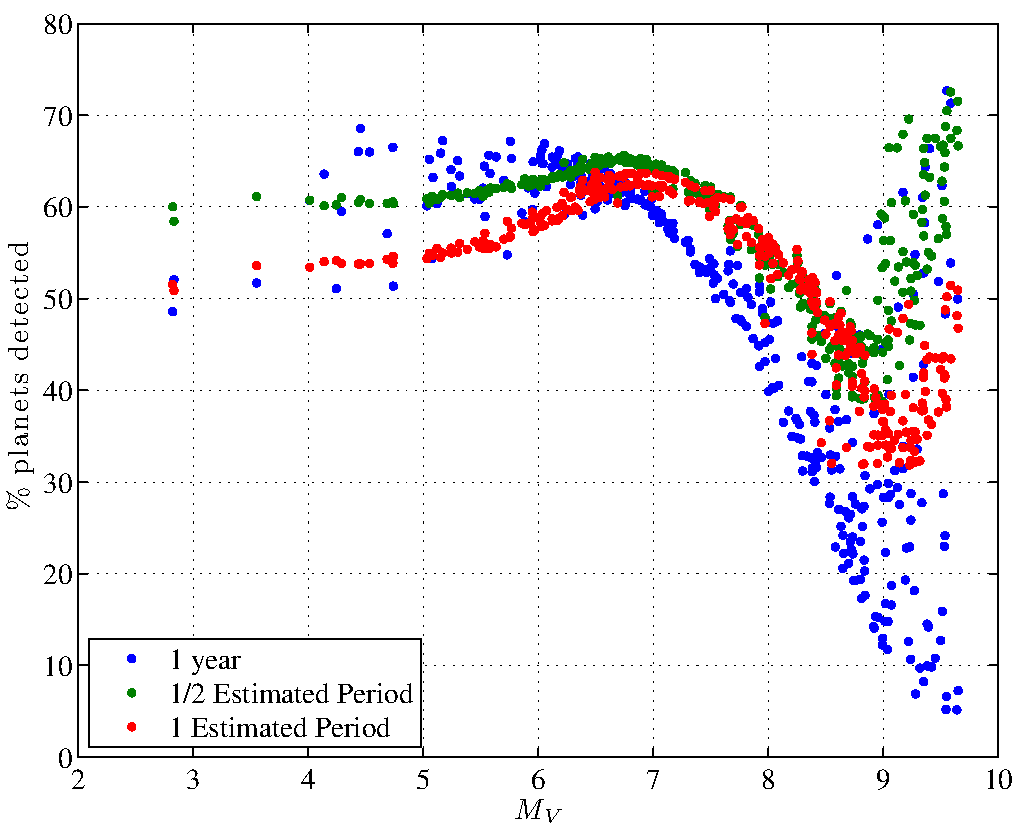
\includegraphics[width = 5.5in]{./figures/revisitStrategies}
 \caption[Revisit timing strategies]{ \label{fig:revisitStrategies} Comparison of revisit detection success rates using the estimated half orbital period, estimated full orbital period, and a constant value of one year, as a function of star absolute magnitude.  The simulated population is $a \in [0.4, 30]$, $e \in [0, 0.8]$, $p \in [0.1, 0.5]$, $R \in [0.7, 11.2]R_\oplus$, with orbits scaled so that planets receive the equivalent flux as they would for a 1$L_\odot$ star.  The constant interval case outperforms the period estimate case only in the case of the brightest stars, where planets are most often visible.}
 \end{figure}

It is important to point out that the return visit strategy may be significantly affected by the detection of multiple planets during the same visit.  If multiple planets are seen at wide angular separations during one observation, assuming that they have small mutual inclinations, it might be safe to assume that the exosystem was being viewed nearly pole-on, and thus would have already captured about as much of the habitable zone as possible, thereby negating the need for future visits if you were only interested in detection and spectral characterization (of course, multiple visits would still be needed for orbital characterizations).  Attempting to estimate the frequency at which multiple detections will occur during single observations is fairly difficult, since it depends completely on the makeup of exosystems.  Our currently small sample of multiple planet system contains a large fraction of `hot jupiters' due to the biases of the detection methods used.  These planets, due to their proximity to their primary stars, would not be detectable with the direct detection instruments studied here, and thus do not constitute a good test.  Instead, we can take our own solar system, and simulate randomly timed observations with the plane of the ecliptic randomly oriented with respect to the line of sight, and the system barycenter located a random distance from the observer.   Doing so for distances between 10 and 30 parsecs, with observations randomly placed in a 5 year window, and using a 75mas IWA instrument with a limiting $\Delta$mag of 26, produces slightly over 30\% of observations in which more than one planet could be seen, with only 4\% in which more than two are detectable.  

Furthermore, because Jupiter and Saturn are so highly detectable, the system orientation was classified close to pole-on (less than 10 degrees rotation) in only 20\% of these cases.  Thus, while it is probable that multiple detections will occur within single observations of systems structured somewhat like our own, this does not guarantee that we will be able to discount systems after a  single visit.  Even in cases where we will have good constraints on the exosystem inclination (i.e., when at least one of the planets detected is clearly in the inner system), one could argue that repeat observations as scheduled by the algorithm used here can be useful.  First, they will likely be required for confirmation---re-detecting a planet when it has moved noticeably on its orbit makes a much stronger case that the original detection was not of a background object or structure in the zodiacal dust. Second, while our solar system has very small mutual inclinations, we cannot discount the possibility that there exist stable exosystems with high mutual inclinations \citep{libert2007exoplanetary}.  

Another very important question that cannot be addressed with the single-planet system model is: in cases where a repeat observation of a target system where a planet has been previously discovered yields another detection, how can we determine whether we are seeing the same planet as before, or a new one?  This is often termed as `confusion' and can lead to significant inaccuracies in the gathered data set.  It is also  extremely important to rule out confusion when attempting to  confirm that initial detections really represent bodies that belong to the target star system, and to ensure that the data points we use for orbit fitting actually belong to the same data set.

One way to answer this question is to apply simple Bayesian theory.  The probability that a current observation is of the same planet as a previous one is given by
\begin{equation}\label{eq:bayesMultiPlanet}
P\left[\mathbf{p}_k | \mathbf{p}_{k-1},  \{\mathbf{p}_k,\mathbf{p}_{k-1}\} \in \mathbf{\gamma}_{k-1}\right] = \frac{P\left[\mathbf{p}_{k-1},\{\mathbf{p}_k,\mathbf{p}_{k-1}\} \in \mathbf{\gamma}_{k-1} | \mathbf{p}_{k}\right] P\left[(\mathbf{p}_k\right]}{P\left[\mathbf{p}_{k-1}\right]}
\end{equation}
where $\mathbf{p}_i$ is the parameter set recorded in the $i$th observation (i.e., star-planet separation and difference in magnitude), and $\mathbf{\gamma}_i$ is the space of all possible parameter sets belonging to a single planet that includes $\mathbf{p}_i$.  The likelihood, $p(\mathbf{p}_{k-1},\{\mathbf{p}_k,\mathbf{p}_{k-1}\} \in \mathbf{\gamma}_{k-1} | \mathbf{p}_{k})$, is approximately equivalent to the goodness-of-fit of a stable orbit to both data points, while the priors, $p(\mathbf{p}_k)$ and $p(\mathbf{p}_{k-1})$, can be calculated from the completeness distribution of the target star \citep{savransky2010occulting}.  This technique is demonstrated in \S\ref{sec:validation}.

\section{Simulation Methodology}
\refeq{eq:detIntTime} allows us to calculate how much time we need to spend integrating before we can assume, with a specific confidence, that no planet exists (or is currently observable by our instrument).  In the simulation framework, we calculate the required integration time for each target star assuming a planet observed at the IWA and the instrument's limiting $\Delta$mag.  For missed and null detections, this time value is used as the actual integration time (in a real mission, this would be the time spent integrating before moving on to the next target).  For detections, the integration time is recalculated based on the simulated planet's orbital position, using the actual separation (and throughput) and $\Delta$mag of the planet at the time of the observation (in a real mission, this would be the point when a detection could be confirmed via a bayesian technique and integration would either be stopped, or switched to spectral characterization).  False alarms (when no observable planet exists) and missed detections (when there is an observable planet) are generated at the rate determined by the FAP and MDP values used in calculating the integration time in \refeq{eq:detIntTime}.  Typically, the FAP and MDP are set to 1\% divided by the expected number of observations for the whole mission, and 0.1\%, respectively, which tends to yield zero missed detections and at most one or two false alarms per mission simulation for all of the cases considered in \S\ref{sec:case_studies}.

\begin{figure}[ht]
\centering
   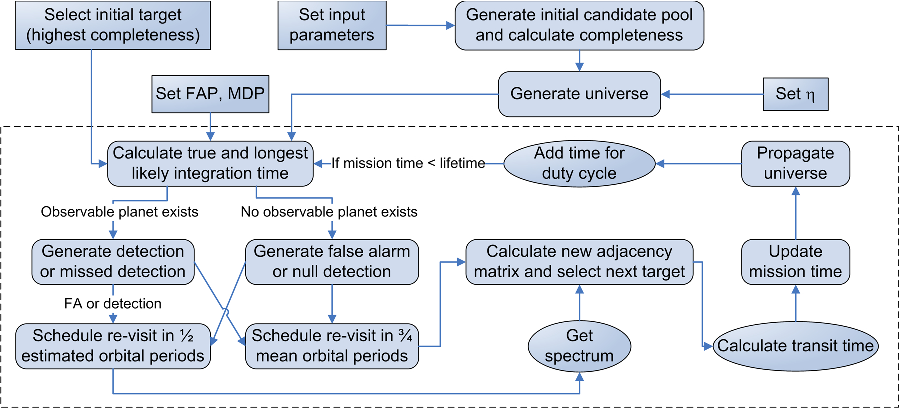
\includegraphics[width = 6in]{./figures/simFlowchart}
 \caption[Simulation Flowchart]{ \label{fig:flowchart} Flowchart of simulation framework.  Ellipses represent optional steps determined by the specific instrument or rule set.}
 \end{figure}
\reffig{fig:flowchart} shows a flowchart for the full implementation of the simulation framework.  The basic steps of the simulation are as follows:
\begin{enumerate}
\item Generate single visit completeness values for all stars for the assumed planetary population. 
\item Generate target list based on given parameters and single visit completeness.  Assign planets to some subset of the target list based on selected planet frequency.
\item Generate the observatory orbit (including Earth rotation for ground-based instruments) and find all times over mission lifetime when targets will be observable.
\item Calculate maximum integration times for each target assuming planets at the IWA and $\Delta$mag$_0$, with the highest possible exo-zodi level.
\item Select initial target by choosing currently observable target with highest single visit completeness.
\item While the current time is less than the mission lifetime:
\begin{itemize}
\item Update visited list with current target.
\item If there is an occulter, calculate the disturbance forces acting on it at its present location.
\item If a planet exists in the target system, find its current angle on the sky and $\Delta$mag, the amount of  integration time required to detect it at the false alarm and missed detection probabilities being used.  If the planet will remain outside the IWA and be brighter than $\Delta$mag$_0$ for this amount of time, it is observable.  Otherwise, use the maximum integration time for this target, and increment the mission time by the integration time. If there is an occulter, decrement the spacecraft mass for stationkeeping for the integration.
\item If the planet is observable, generate a false negative (with probability of the missed detection rate) or a detection (with the complement probability 1).  If the planet is not observable, generate a false positive (with probability of the false positive rate) or a non-detection.
\item If a detection or false positive has occurred, and spectral characterization is called for, calculate the integration time required.  If the target star will be out of the keep-out for this amount of time, increment the mission time (and, if there is an occulter, decrement the spacecraft mass).  If the planet is observable for this whole time period, record a successful spectral characterization.  For coronagraphs, calculate and record the maximum observable wavelength.  If using a multiple distance occulter, attempt the second characterization in the same way.  
\item Add star and revisit time to the revisit list.
\item Calculate new cost function matrix based on current time and select next target.  If there is an occulter, calculate slew time and decrement spacecraft mass with the amount of fuel used.
\item If a portion of the mission is devoted to some other science, increment mission time by proportional amount.  Add spacecraft settling time before beginning next observation.
\item Propagate all of the planets in all target systems along their orbits by the total amount of time that has elapsed in this iteration step.
\end{itemize}
\end{enumerate}

At each step of this iteration, the state of the mission and all activities is encoded using the variables listed in Appendix \ref{app:DRMencoding}.  To check whether the final path generated is reasonable, and to allow for easier visualization of a whole mission timeline,  we can plot the sequence of observations on a map of the sky.  A sample of this is shown in Figure \ref{fig:theia_DRM}.  Because of the large number of inputs and parameters required to run a simulation, a graphical front-end was created to manage all of these.  \reffig{fig:DRMconstructor} shows the main panel of the application, called `DRMconstructor' used for setting up and running simulations. 
%
\begin{figure}[ht]
\centering
   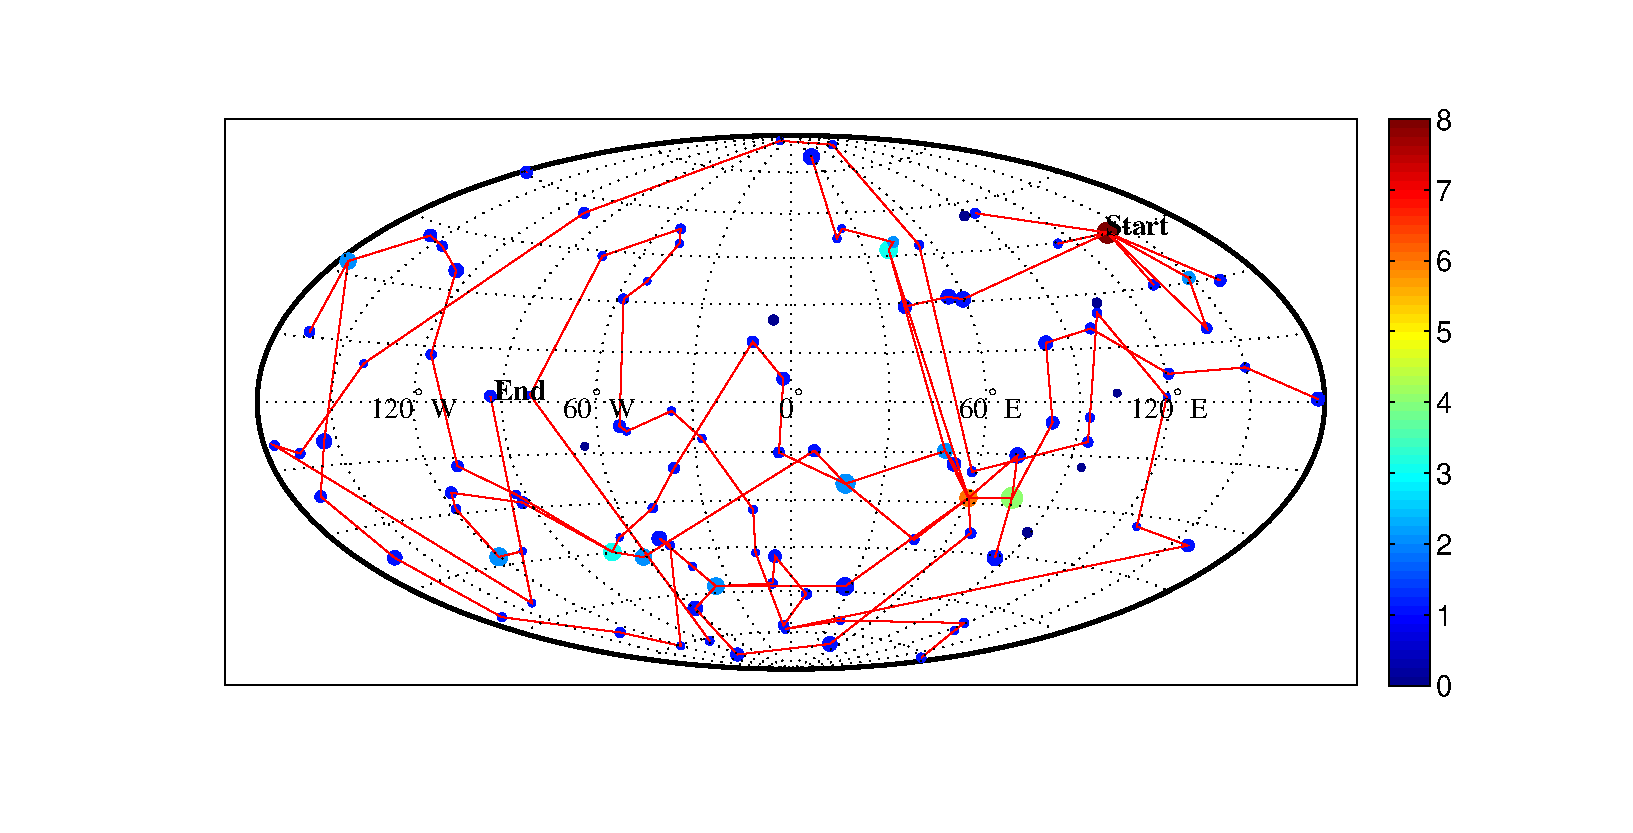
\includegraphics[width = 6in,clip=true,trim=1.2in 0.75in 0.9in 0.5in]{./figures/theia_DRM}
 \caption[Sample auto-generated DRM]{ \label{fig:theia_DRM} Visualization of an automatically generated sequence of observations. Points represent target stars, with size correlated with single visit completeness (i.e., the larger the point, the higher its single visit completeness). The color scale represents the number of observations made of a system in this simulation.  Note that some systems get many visits not because of their high completeness, but because they are well located on the sky.}
 \end{figure}
 \begin{figure}[ht]
\centering
   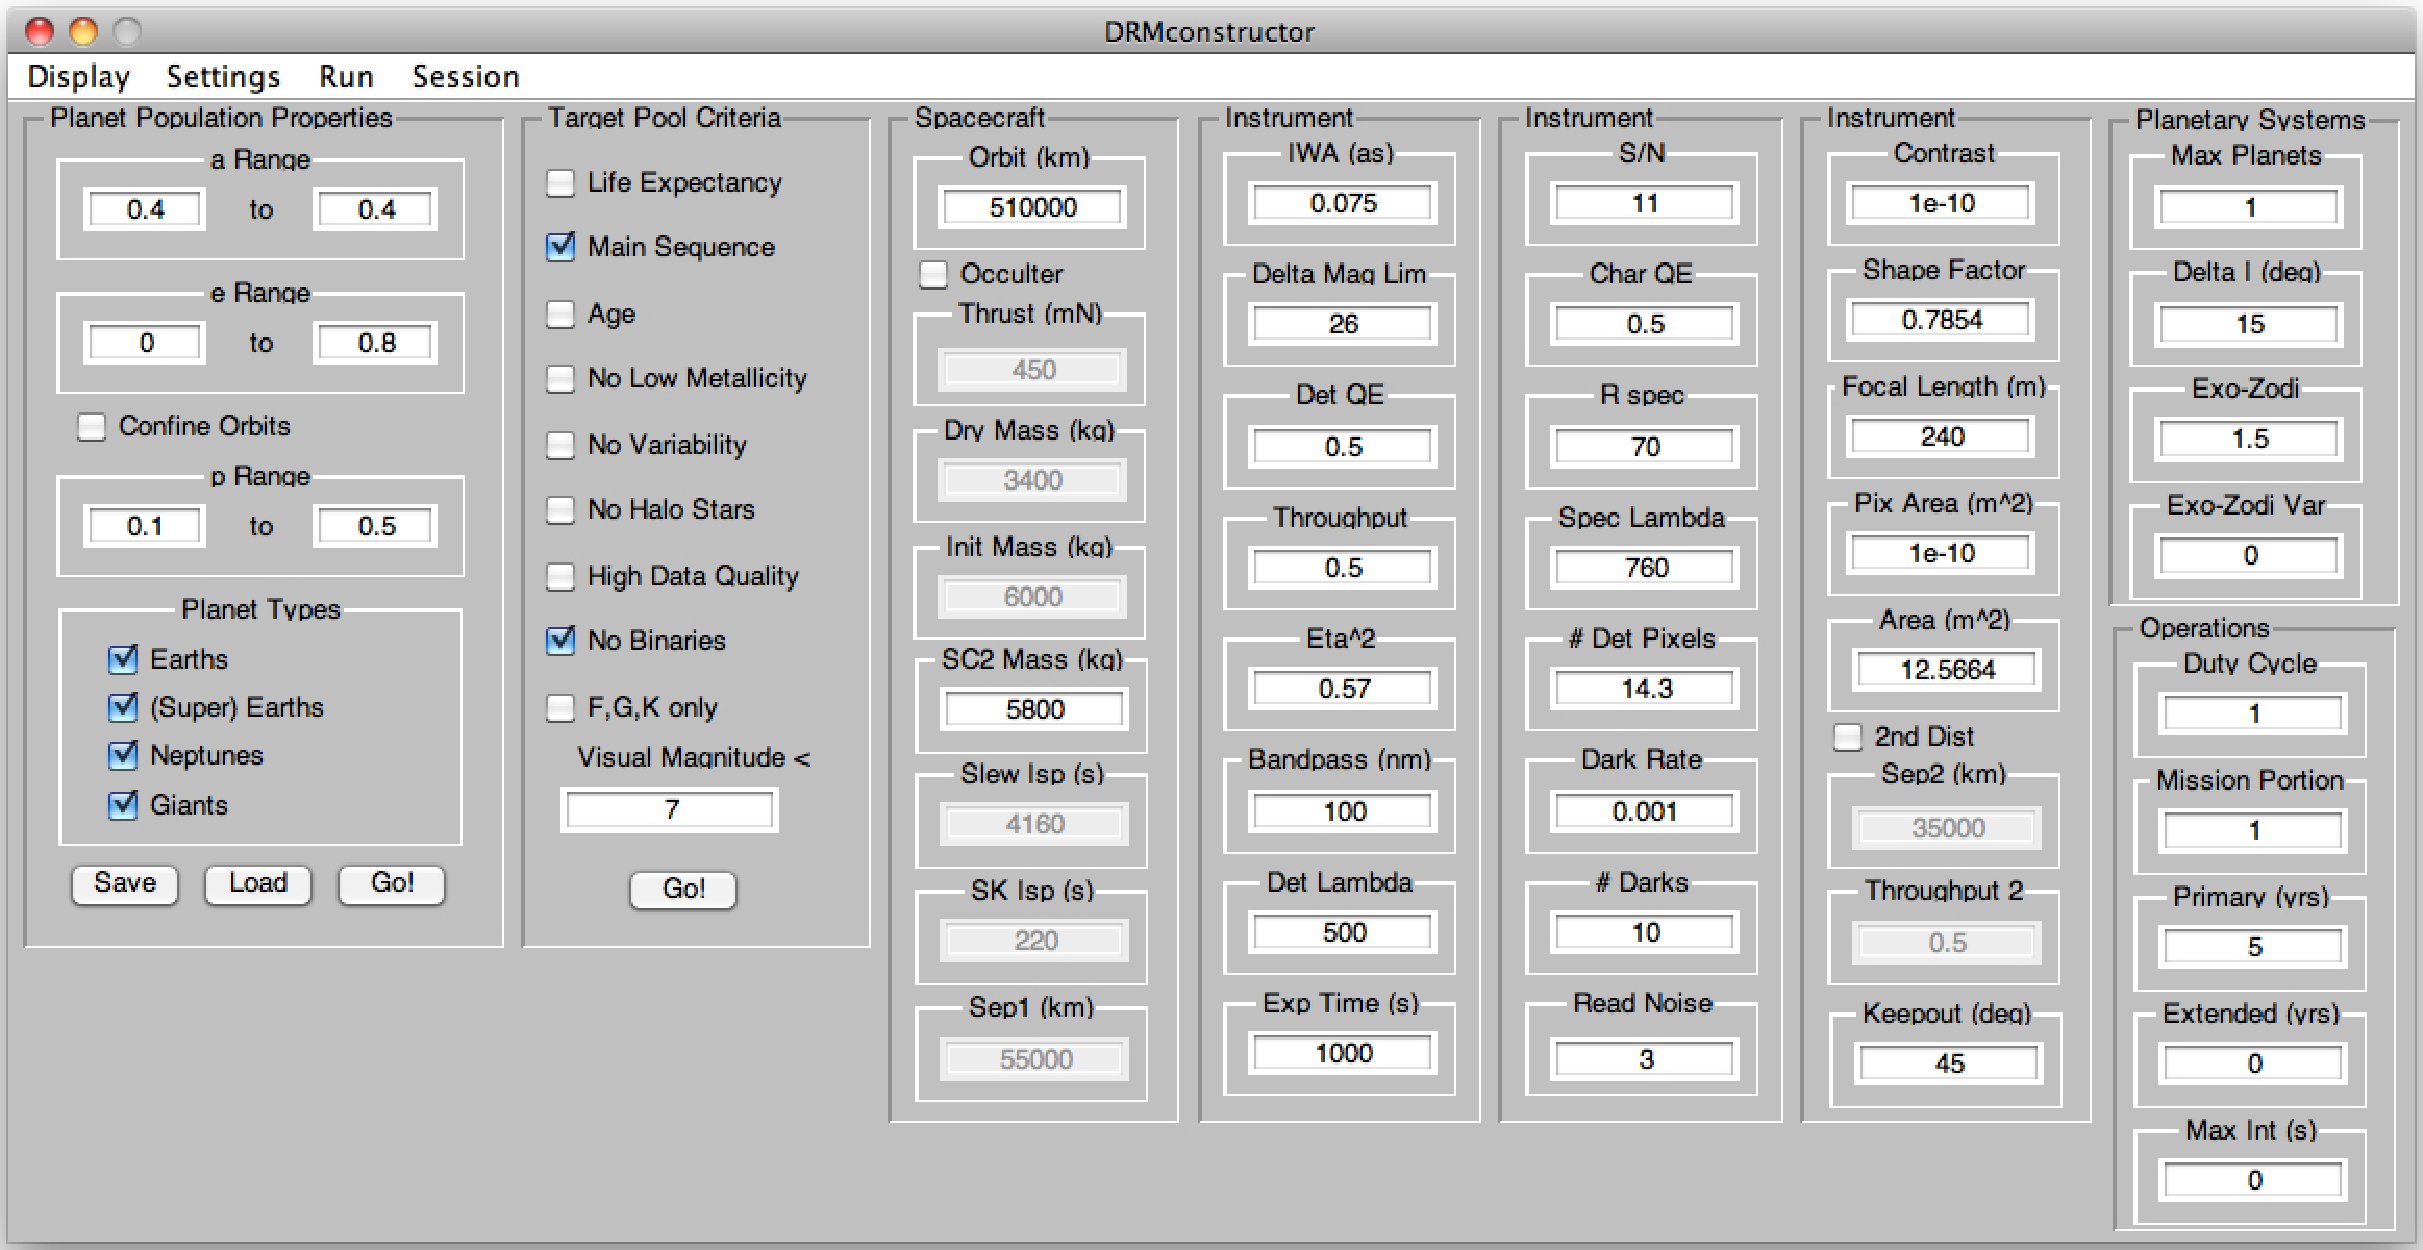
\includegraphics[width = 6in]{./figures/DRMconstructor}
 \caption[DRMconstructor]{ \label{fig:DRMconstructor} Graphical front-end of the DRMconstructor simulation utility.}
 \end{figure}

Because this process must be repeated many times in order to generate the ensembles of mission timelines required to calculate the distributions of various performance metrics, it is reasonable to attempt to parallelize as much of it as possible.  Fortunately, as each timeline can be evaluated independently of the others, generation of an ensemble is inherently parallelizable to an arbitrary number of processes by simply assigning each new simulation to the first available  process thread, or by pre-assigning an equal number of simulations to each thread.  The simulations in \S\ref{sec:case_studies} were all carried out on a multi-core, multi-processor machine, utilizing a maximum of 8 concurrent threads and a single local scheduler, but the basic framework can be easily extended to large distributed computing environments by substituting a remote scheduler.

\section{Case Studies}\label{sec:case_studies}

The purpose of this section is to demonstrate completed analyses of direct detection missions using the techniques described throughout this chapter.  Because one of the most important goals of planet-finding is the discovery of Earth-like planets, we use, as the base case, populations of Earth-twins.  Unless otherwise noted, the simulated systems in this section are populated with Earth-twins distributed throughout their habitable zones (defined as $a \in [0.7, 1.5]\sqrt{L}$ and $e < 0.35$) with either zero or one planets per system.  The term `Earth-twin' indicates planets of the radius and mass of the Earth, with a constant albedo of 0.22 (this value was selected to conform with previous studies, including \citet{lindler2007}) with isotropically distributed orbital orientations.  Exo-zodi levels are taken to be constant, with $\mu = 1.55$ to correspond to the historical average zodi brightness \citep{kuchner2008}.  When spectral characterization is possible, default mission rules call for one complete spectrum to be collected for each unique planet (meaning that spectral characterization is not performed during revisits unless a full spectrum was not taken at the initial detection, or the mission rules are modified). The settling time (i.e., the time to acquire a new target and begin observing) for all spacecraft is taken to be 24 hours. A full listing of the default parameters is available in Appendix \ref{app:defSets}.

All of the spacecraft are assumed to reside on a halo orbit about the Earth-sun L2 point.  For occulter systems (except in the case of O$_3$, see below) the telescope is placed on the halo orbit, which is assumed to be stable enough that only minor thrust corrections are required to keep the spacecraft on the orbit over the life of the mission.  The orbit of the occulter spacecraft, however, must be actively adjusted throughout the course of the mission, both to reposition the spacecraft for observing new targets (slewing), and to maintain precise alignment between the two spacecraft (stationkeeping).  The methods for generating stable halo orbits, as well as techniques for optimal point-to-point transfers about these orbits are developed in \citet{kolemen2008thesis}.  An example of the nominal halo orbit (510000 km in the azimuthal direction) is shown in \reffig{fig:halo_orbit}.
\begin{figure}[ht]
\centering
   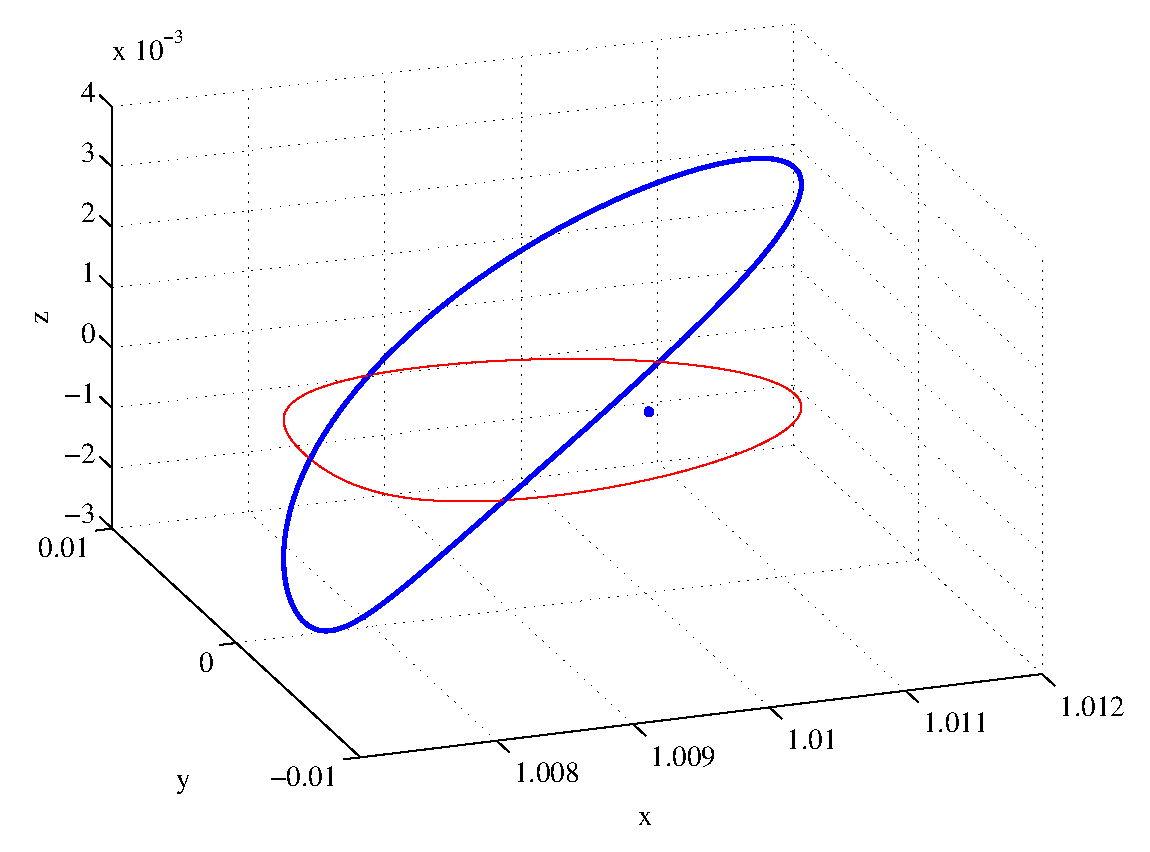
\includegraphics[width = 5.5in]{./figures/halo_orbit}
 \caption[Halo orbit]{ \label{fig:halo_orbit} Nominal halo orbit (510000 km azimuthal radius).  The blue point is the Earth-sun L2 point, while the red curve is projection of the orbit into the plane of the ecliptic.  Note that the out of plane component of the orbit is much smaller than the in-plane components.  Units are AU and the coordinate system is heliocentric, with $z$ perpendicular to the ecliptic, and $x$ increasing away from the sun}
 \end{figure}

Among the instruments and missions considered, some represent specific mission concepts that are relatively well developed (with a large number of design details and requirements available for the simulation), whereas some represent more generalized missions intended for high-level comparisons of different instrument types.  The various concepts are listed below, along with the basic parameters used to describe each.  Specific settings that were varied for certain instruments for particular tests or to maximize different metrics are detailed along with the simulation results in the following sections.
\begin{enumerate}
\item Generalized Single-Distance Occulter (SDO$\addsymbol{SDO}{Single-Distance Occulter}$) - The baseline occulter mission consisting of a circular aperture telescope and an occulter spacecraft operating at one separation distance from the telescope.  This type of occulter is designed to provide high contrast across the entire spectral band and is therefore larger than occulters designed to provide equivalent contrast over smaller bands \citep{cady2010design}.  Different propulsion systems may be employed for different designs (especially at differing telescope scales), but the baseline uses the same propulsion system as THEIA (see below).  Multiple designs have been created for telescopes of various aperture sizes, and are detailed in \reftable{table:occulters}.  
\item Generalized Multiple-Distance Occulter (MDO$\addsymbol{MDO}{Multiple-Distance Occulter}$) - Essentially equivalent to the generalized SDO, the MDO is designed to achieve high contrast over two (roughly) equal bands at different distances.  The majority of these designs use a second separation distance equal to half of the original, thereby operating at double the IWA for higher wavelengths.  See \reftable{table:occulters} for details.
\item Generalized Coronagraph - The baseline design for self-contained coronagraphs.  While not specifically modeling any one coronagraph type, this represents any of a number of high-throughput, low-IWA coronagraphs currently under development \citep{guyon2006theoretical,groff2010progress}.  Typical IWAs are either 2 or 3 $\lambda/D$, which corresponds to between 26 and 103 mas for a 4 m telescope---comparable to the geometric IWA of the baseline occulter for a 4 m aperture and detections in the V band.  By default, the coronagraph missions devote 50\% of their time to planet-finding activities (as opposed to coronagraphs, which typically use less than 33\%).
\item Telescope for Habitable Exoplanets and Interstellar/Intergalactic Astronomy (THEIA) Exoplanet Characterizer (XPC) \citep{spergel2009} - An MDO for a  4 m telescope developed as a flagship mission class concept study whose primary goal is the detection and spectral characterization of Earth-like planets.  The mission design yields high-contrast spectral capability over the 250 - 1000 nm band, split into two sub-bands, with geometric IWAs of 75 and 118 mas, respectively.  This allows for the detection of molecular oxygen at high confidence levels.  The mission rules developed to address the primary mission goal call for attempting to maximize the number of unique detections while heavily biasing the scheduling towards multiple revisits to a small candidate sub-pool of good targets (ones with previously discovered bright planets) to ensure at least a few orbit fits. A full spectrum (to resolution of R=70 at 760 nm) is also required for each unique detection.  The THEIA occulter uses paired NEXT ion thrusters \citep{patterson2002next} to provide up to 450 mN of thrust at a specific impulse of 4160 s.  Stationkeeping is performed with hydrazine thrusters with $I_{sp} = 220$ s.  The separate stationkeeping system was added due to concerns that the plumes produced by the electric propulsion system would be bright enough to interfere with observations.
\item Occulting Ozone Observatory (O$_3$) - An SDO or MDO for a 1.1 - 2 m telescope developed as part of a mission concept study aimed at finding a less expensive (\midtilde\$1 billion) planet-finder.  While O$_3$ can cover the same band as THEIA, the smaller aperture makes high resolution spectroscopy unreasonable, so O$_3$ focuses on band photometry, while retaining the ability to detect ozone, another biomarker \citep{heap2010detecting}.  When operating as an SDO, O$_3$ does not have photometric sensitivity beyond 550nm.  As an MDO, O$_3$ can operate in the `blue' band (250 - 550 nm) or the `red' band (500 - 1100 nm).  See \reftable{tbl:O3filters} for details on the photometric bands \citep{savransky2010occulting}.  Unlike the other occulters, O$_3$'s occulter spacecraft remains in an unperturbed orbit while the telescope spacecraft is repositioned between observations, using chemical thrusters providing a thrust of 500 mN at an $I_{sp}$ of 600 s.
\end{enumerate} 

\begin{table}[ht]
\caption{Occulter Designs. \label{table:occulters}}
\begin{center}
\begin{tabular}{ c c c c c }
\hline\hline
Telescope & Occulter &  50\% Throughput & Starshade & Petal\\
 Diameter  (m) & Type &  IWA (mas) & Mass (kg) & Length (m)\\
\hline
2 & SDO/MDO\tnote{\textasteriskcentered} & 69.6 & 2300 & 7\\
\hline
\multirow{2}{*}{4} & SDO  & 59 & 4200 & 19\\
			       &  MDO\tnote{\textdaggerdbl} & 57.5 & 3370 & 10\\
			       \hline
\multirow{2}{*}{8} & SDO & 56 & 7180 & 24\\
			       &  MDO  & 53 & 4915 & 13.5\\
			       \hline
16m & MDO & 47 & 10022 & 21.5\\		       
\hline
\end{tabular}

\medskip

\begin{threeparttable}[b]
\begin{tabular}{ c c c c }
\hline\hline
Telescope & Occulter & Starshade & Separation\\
 Diameter  (m) & Type &  Radius (m) & Distance (km)\tnote{\textdagger} \\
\hline
2 & SDO/MDO\tnote{\textasteriskcentered} & 17 & 38960/19480 \\
\hline
\multirow{2}{*}{4} & SDO & 25.6 & 70400 \\
			       &  MDO\tnote{\textdaggerdbl} & 20 & 55000/35000 \\
			       \hline
\multirow{2}{*}{8} & SDO & 35.2 & 96800\\
			       &  MDO & 27.2 & 74800/52360 \\
			       \hline
16m & MDO & 43.2 & 118800/83160 \\		       
\hline
\end{tabular}
\begin{tablenotes}
  \item [\textdagger] For MDOs, the first separation distance is used for covering 250-700nm, and the second for 700-1000 nm, except for O$_3$, which is split into the `blue' and `red' bands in \reftable{tbl:O3filters}.
    \item [\textasteriskcentered] This is the 1.5 - 2 m $O_3$ design.
    \item [\textdaggerdbl] This is the final design for THEIA.  The same design can also be used with a 1 m telescope.
   \end{tablenotes}
 \end{threeparttable}
 
 \end{center}
\end{table}

\begin{table}[ht]
\caption{O$_3$ filters. \label{tbl:O3filters}}
\begin{center}
\begin{threeparttable}[b]
\begin{tabular*}{0.8\textwidth}{@{}@{\extracolsep{\fill}} c c c @{}}
\hline\hline
\multirow{2}{*}{Filter \#} & \multicolumn{2}{c}{Bandpass ($\mu$)} \\
  & Blue & Red\\
\hline
1 & 0.25 - 0.31 & 0.5 - 0.7 \\
2 & 0.31 - 0.4 & 0.7 - 0.9 \\
3 & 0.4 - 0.48 & 0.9 - 1.1 \\
4 & 0.48 - 0.55 & Narrowband\tnote{\textdagger} \\      
\hline
\end{tabular*}
\begin{tablenotes}
    \item [\textdagger] The specific narrowband filter selection will be informed by results from transit photometry, which should help pinpoint the most interesting and common giant planet near-IR features, but will most likely coincide with a methane absorption feature.
   \end{tablenotes}
 \end{threeparttable}
 \end{center}
\end{table}

The point spread functions for the optical systems of these instruments are generated using different algorithms. Throughput curves for coronagraphs are created by sequentially generating tilted wavefronts at the telescope aperture and applying propagation algorithms to these.  For occulters, we use the Bessel expansion described in \citet{vanderbei2007} via a fast algorithm to calculate the electric field at the aperture of the telescope, assuming an incident plane wave on the occulter.  The field at the telescope aperture following a tilted incident wave may be related to the field from an incident plane wave by:
\begin{equation}
    E_{\mathrm{tilt}}(x, y) = e^{-i k \sin{\alpha} x} e^{i k z \cos{\alpha}} E(x + \sin{\alpha} z, y)
\end{equation}
which holds for small angles and allows the Bessel expansion for plane waves to be used. This field may then be fed into the appropriate propagation scheme.  (Propagation through the telescope with no coronagraph is treated as just a Fourier transform.)  In general, we prefer to examine throughput in terms of total energy in pupil planes rather than image planes, as the finite extent of the pupil planes ensures a more accurate measure of energy \citep{kasdin2006}.  It is important to note that the throughput curves shown in \reffig{fig:throughputs} are idealized, and achieving these levels of performance will require meeting exacting manufacturing and positioning tolerances for the occulters, and very precise wavefront control for the coronagraphs.
 \begin{figure}[ht!]
 \centering
 \subfigure[SDO Throughput]{ 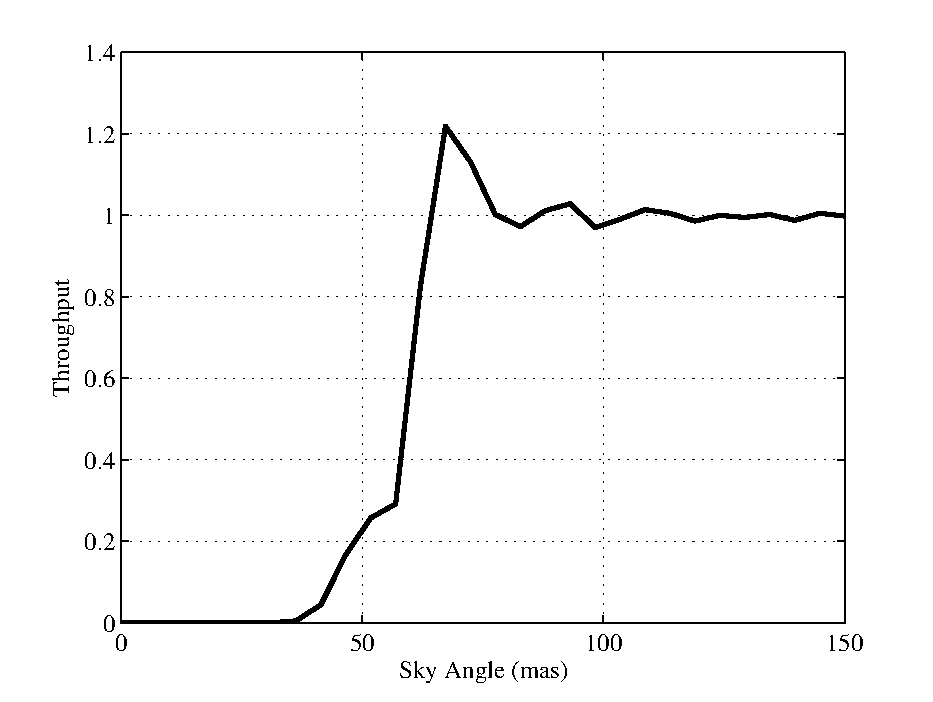
\includegraphics[width = 2.8in,clip=true,trim=0.25in 0in 0.25in 0in]{./figures/sdocculter_throughput}  \label{fig:sdocculter_throughput} }
 \subfigure[THEIA throughput]{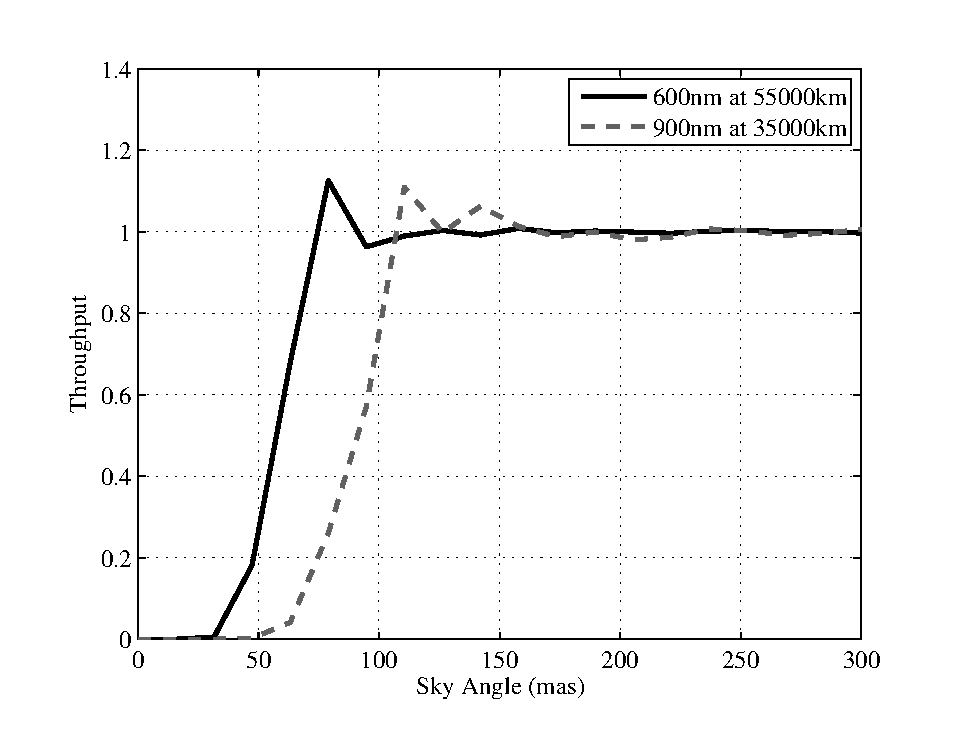
\includegraphics[width =  2.8in,clip=true,trim=0.25in 0in 0.25in 0in]{./figures/theia_throughput} \label{fig:theia_throughput}}\\
 \subfigure[O$_3$ throughput]{ 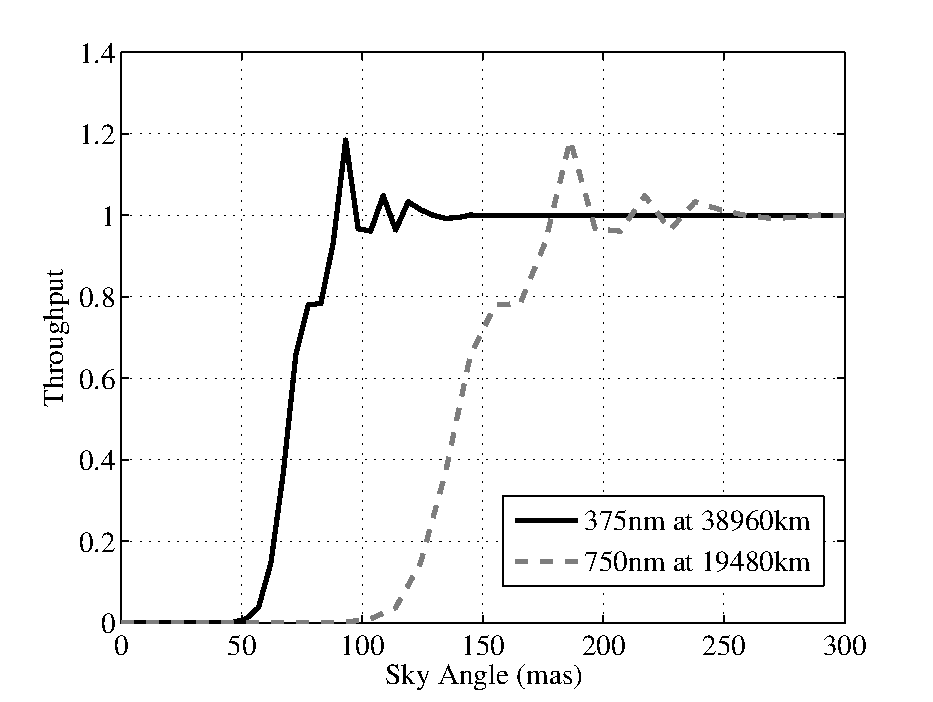
\includegraphics[width= 2.8in,clip=true,trim=0.25in 0in 0.25in 0in]{./figures/O3_throughput}  \label{fig:O3_throughput} }
 \subfigure[Coronagraph Throughput]{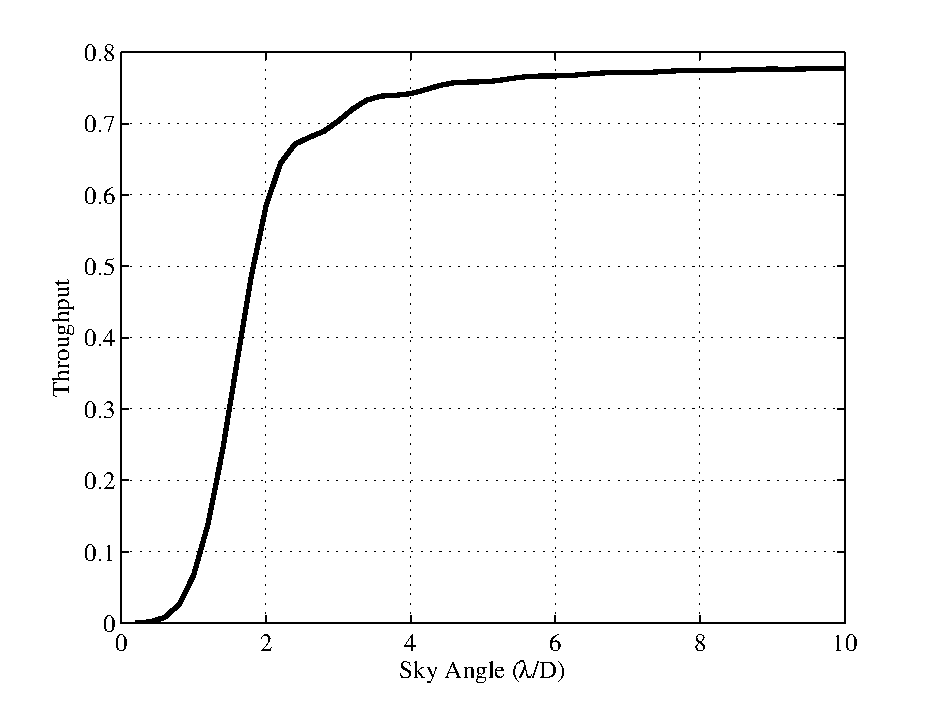
\includegraphics[width =  2.8in,clip=true,trim=0.25in 0in 0.25in 0in]{./figures/coron_throughput} \label{fig:coron_throughput}}
 \caption[Throughput Curves]{\label{fig:throughputs} Throughputs as functions of angle on the sky (units of mas for occulters occulters and $\lambda/D$ for coronagraphs). The throughput may be greater than unity for occulters since at certain angular separations, the occulter petals will send planet light into the telescope aperture that would otherwise have bypassed it. Data for (d) was provided by L. Pueyo (Personal Communication, 2009).}
\end{figure}

\subsection{Validation}\label{sec:validation}
Before we can use the results from mission simulations based on the decision modeling described in \S\ref{sec:scheduling}, it is necessary to determine whether the cost function described by \refeq{eq:costfunc}  actually produces optimal (or close to optimal) results.  Of course, the definition of optimality in this case depends entirely on what we want the mission to achieve, and how we prioritize the various science deliverables (i.e., how we set the weight factors $a_i$ in the cost function).  Still, if the cost function operates as designed, and all weights are set to be equal, we would expect the resulting simulations to maximize science yield while minimizing operational cost.  Since there is a direct tradeoff between time spent on new detections and time spent on characterizations, and between fuel use and available observation time, we do not expect a globally optimal solution for any of these.  Instead, we want to always be able to find the easily detectable planets in every universe, and to get orbits and spectra for as many of these as time permits, while reducing fuel use in designs with occulters.  

To test whether the framework described here accomplishes this, we can generate a `ground truth' case in the form of the distribution of all possible mission scenarios with a fixed set of target systems.  To do so, we generate one single universe, and compare the results of the mission simulation for this universe using our automated decision modeling to mission simulations with randomly generated visit orders.  Specifically, rather than using our decision modeling algorithm to decide on the next target, we simply select one at random from the list of targets currently outside of the keep-out zones.  By running this randomized visit order mission on the same universe multiple times, we can map the space of possible observing sequences and find a distribution of mission results.  We can also use a modified version of our framework that always selects the next available highest completeness target, rather than using the cost function in \refeq{eq:costfunc}.

\reffig{fig:optim_hists} shows the resulting histograms for the number of unique planet detections and successful spectral characterizations found from running 1000 randomized visit order missions on a single universe with $\eta_\oplus = 0.5$, using the THEIA and 2$\lambda/D$ coronagraph mission concepts.  On top of these, we have the results of the missions produced by the decision modeling algorithm with a depth of search ($k$) of either 3 or 1, and the results of the mission which only considers completeness in selecting visit order.  
For THEIA, using a $k$ of 3 and 1 produces the same values for both these metrics, whereas the $k=3$ case outperforms the $k=1$ case in terms of unique detections for the coronagraph. All cases using the scheduling algorithm described in \S\ref{sec:scheduling} outperform schedules based on just completeness.
\begin{figure}[ht!]
\centering
2 $\lambda/D$ Coronagraph\\
 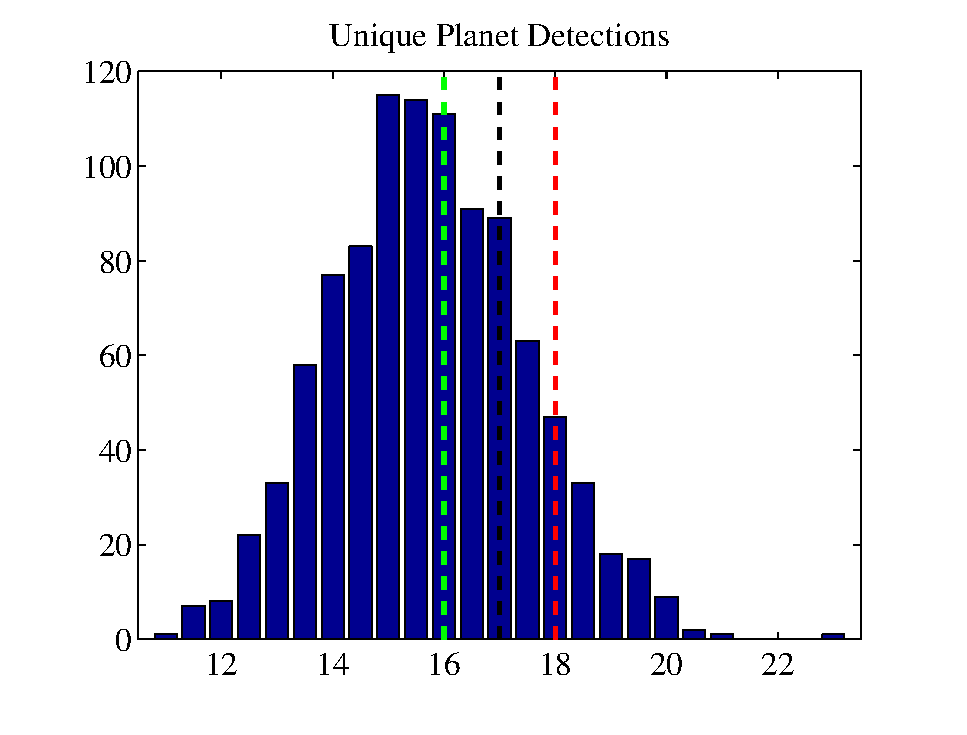
\includegraphics[width = 2.8in,clip=true,trim=0.4in 0in 0.5in 0in]{./figures/optimhistsa}
 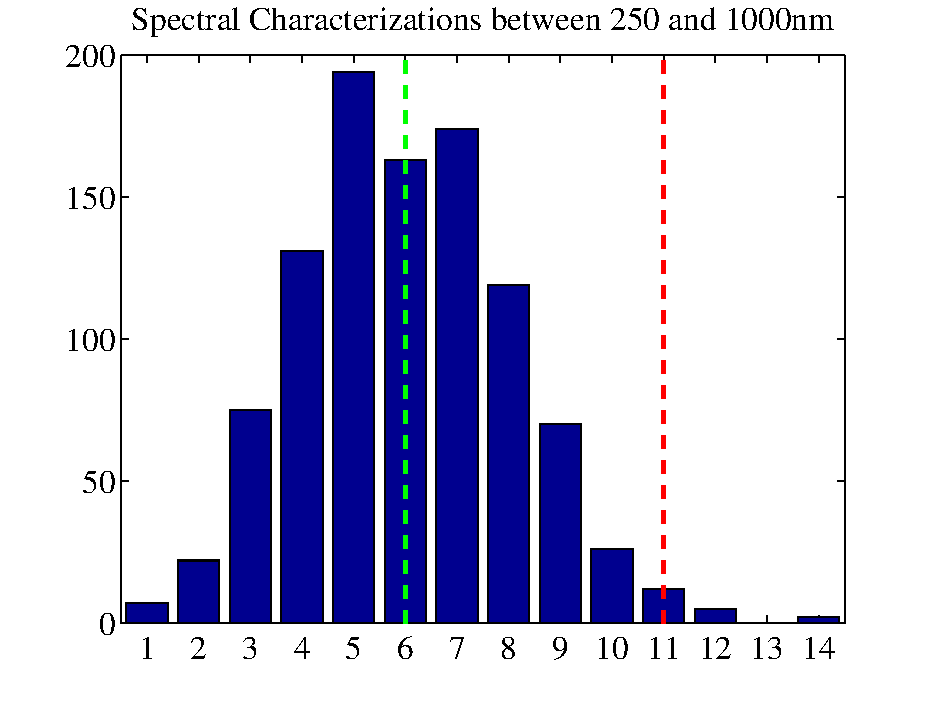
\includegraphics[width = 2.8in,clip=true,trim=0.4in 0in 0.5in 0in]{./figures/optimhistsb}\\
 THEIA\\
  \includegraphics[width = 2.8in,clip=true,trim=0.4in 0in 0.5in 0in]{./figures/optimhistsc}
   \includegraphics[width = 2.8in,clip=true,trim=0.4in 0in 0.5in 0in]{./figures/optimhistsd}
 \caption[Science yield from automated and randomized visit order]{ \label{fig:optim_hists} Comparison of science yield from automated and randomized visit order selection for 2 $\lambda/D$ coronagraph (top row) and THEIA (bottom row).  Blue bars are histograms of results from 1000 mission simulations using randomized visit order. Black dashed lines are results from the automated visit order with depth of search $k = 1$, red lines are results for automated visit order with $k = 3$, and  green lines represent timelines generated by selecting the next available highest completeness target.  In the spectral characterizations for the coronagraph, and both metrics for THEIA, the $k=1$ and $k=3$ cases produced identical results.}
 \end{figure}
 
\reffig{fig:optim_fuelvudets} shows a scatterplot of THEIA occulter fuel use vs.~the number of unique planets found for the 1000 randomized visit order missions and the automated visit order missions.  Here we do see a difference between the $k = 3$ and $k = 1$ simulations, with $k = 1$ producing a mission timeline where more fuel is used.  We compare only the amount of fuel used in slews, rather than total fuel use, since the stationkeeping fuel is directly linked to the number of observations and spectra and is automatically maximized along with these metrics.  This validation technique was applied to multiple randomly generated universes, with varying values of $\eta_\oplus$, producing similar results in each case.
\begin{figure}[ht]
\centering
\includegraphics[width = 5in]{./figures/optim_fuelvudets}
 \caption[THEIA occulter propellant use]{ \label{fig:optim_fuelvudets} THEIA occulter propellant use (in kg) vs.~the number of unique planet detections for 1000 mission simulations using randomized visit order in one simulated universe.  The red point represents the mission timeline generated using the automated visit order for the same universe for $k = 3$, and the black point for $k = 1$.  The green point represents the timeline generated by selecting the next available highest completeness target.}
 \end{figure}

These results show that the automated mission does not represent a global optimum for these metrics.  There are a small number of missions which find more unique planets, or get more spectra.  However, we can see that the automated mission does a very good job of balancing these metrics and maximizing (or minimizing, in the case of fuel use) them jointly.  Allowing for the fact that the automated mission needs to be generated only once per universe, whereas a random walk search for local optima takes many trials, the benefits and efficiency of this approach become quite clear.  In terms of real mission planning, a random walk approach is simply not an option (since we only get one chance at scheduling the mission).  We also see that even when using a $k > 1$ (looking multiple steps into the future) gives us the same science yield as only considering one step, we still end up with a lower occulter fuel cost.  Finally, it is important to note that the margin between the unique planet detections using our scheduling algorithm versus the selection of the next available highest completeness target is smaller for the coronagraph than for THEIA, and is further from the tail of the distribution of randomized visit orders.  This is because the values for $a_i$ were fixed across all of the simulations here, and the $k$ values used are actually quite low for coronagraphs.  Optimizing the weights specifically for coronagraphs and using higher $k$ values produces improvements comparable to those seen in the occulter cases.

\begin{figure}[ht]
\centering
\includegraphics[width = 6in]{./figures/burnin}
 \caption[Science yield metric statistics as a function of ensemble size]{ \label{fig:burnin} Means and standard deviations for four metrics (total number of stars observed, number of unique stars observed, total number of planetary detections, number of unique planets detected) as a function of ensemble size.  These are normalized by the values for the full ensemble of 500 simulations.  Each simulation is of a 5 year THEIA mission with the default parameter set, with a universe of Earth-twins with $\eta_\oplus = 0.5$.}
 \end{figure}
Another important question is how many mission simulations are required so that the statistics extracted from the ensemble are accurate with high confidence.  It is difficult to make the case that the various metrics that we are interested in are approximately normally distributed, especially as many of them (such as the number of unique planets found) are discrete values, making it difficult to select a sample size corresponding to a specific confidence level.  However, this question can be answered empirically, by generating a large number of simulations and calculating distribution moments for the various metrics from subsets of these of varying size.  \reffig{fig:burnin} does exactly this, using 500 simulations of a 5 year THEIA mission with an Earth-twin population at a constant $\eta_\oplus$ of 0.5.  For all of these metrics (and others not plotted here), the sample mean and standard deviation converge to within 5\% of their respective values for the 500 simulation ensemble at around 100 samples.  This holds for a variety of configurations and instrument types, and so 100 samples is taken to be the minimum number required by the simulation framework.

\begin{figure}[ht]
 \centering
   \subfigure[]{\includegraphics[width=2.8in,clip=true,trim=0.4in 0in 0.5in 0in]{./figures/reldetsmult}  \label{fig:reldetsmult}}
   \subfigure[]{\includegraphics[width=2.8in,clip=true,trim=0.4in 0in 0.5in 0in]{./figures/mplanDets} \label{fig:mplandets}}
 \caption[Validation of Bayesian unique planet classification]{Results for 100 mission simulations using the 2 band photometry, 2 m O$_3$ configuration. (a) Total number of detections of each solar system planet analogue, normalized by the frequency with which they were simulated. This is used primarily as a test to ensure the multi-planet simulation capability is working as expected, but can also be useful in determining the relative detectability of the analogues - i.e., if Jupiters and Earths are distributed with equal frequency, O$_3$ should detect 4 times as many Jupiters as Earths, on average. (b) Average number of unique analogues found. Error-bars represent the standard deviation of the distribution. The squares indicate the average number of each analogue type that was included in the simulations.}
\end{figure}
Finally, in order to validate the multiple planet classification algorithm in \refeq{eq:bayesMultiPlanet}, we can generate systems populated with solar system planet analogues (as described in \S\ref{sec:gen_plan_sys}) and have the simulation algorithm classify detections made during repeat observations of targets where planets had previously been detected as newly discovered planets whenever the probability of a repeat detection is less than 50\%.   The test was run using a 44 star target pool with a 2 m telescope O$_3$ configuration and 2 band photometry required for each planet classified as a new detection.  Figure \ref{fig:reldetsmult} shows a histogram of the raw number of detections of each solar system planet analogue, normalized by the frequency with which they were simulated.  This is essentially the same as counting the total number of detections of each planet type in simulations where all of the analogues are selected with equal frequencies, and gives a sense of the relative detectability of the various planets in our solar system. 

As expected, Jupiter and Saturn-like planets, due to their size, relatively high albedo and placement, will be detected much more frequently than any other planet type.  Earths will be detected more frequently than Venus or Mars analogues due to their size and placement, and ice giants like Neptune will be difficult to detect unless they orbit much closer to their stars than Neptune does to the sun.  This histogram also implies that if Earth-twins and Jupiter-twins occur at the same rate in our universe, an observatory like O$_3$ should detect roughly four times as many Jupiters as Earths.  We can also use this data set to estimate the probability that a habitable zone candidate (i.e., a detection with an apparent separation less than the outer edge of the target star's HZ) actually is a habitable zone planet.  We find that if every exosystem was a scaled copy of the solar system, HZ candidates would represent about 22\% of all detections, and would actually be Earth analogues 43\% of the time.  They would be rocky planet analogues (Venus, Earth, or Mars) 83\% of the time, and giant planet analogues (Jupiter, Saturn, or Uranus) 17\% of the time.

Figure \ref{fig:mplandets} shows the average number of each planet analogue classified as unique over 100 simulations.  The algorithm correctly identified planets as new detections in approximately 60\% of applicable cases (detections during repeat observations of targets with prior detections).  This led to the apparent discovery (according to the algorithm's internal bookkeeping) of approximately 45\% of included Earth-like planets, whereas earlier single-planet system studies indicate that this value should be less than 33\%.  At the same time, according to the algorithm's classification, it discovered slightly more Jupiters, on average, than were included in the simulation, while in reality the true average rate of discovery was closer to 85\%. Because of the limited target pool size, each star in the  pool was observed at least once in most of the simulation instances, and the high visibility of Jupiter analogues made them easy to detect.  

\subsection{Results}
For each instrument an ensemble of mission simulations was generated over simulated universes containing only Earth-twin planets, a fixed mission length of 5 years, and fixed target lists selected from a pool of real stars within 30pc of the solar system.  Each ensemble consists of 1000 simulations with varying assumed frequencies of Earth-like planets ($\eta_\oplus$). Figures \ref{fig:compinsts4m} to \ref{fig:compinsts16m} show the median values of the four science yield metrics for the four instrument designs for telescopes with circular apertures of 4, 8 and 16m diameters.  The error-bars represent the one-sided deviations of each distribution.  No SDO was evaluated for the 16m telescope because the starshade is so large that little significant science can be achieved during a 5 year mission with the propulsion system used here.  Results for O$_3$ are plotted separately since O$_3$ does not have a spectral characterization capability, making it difficult to compare directly with the other instruments that do.  The lines in the various plots represent median values for 100 simulations at each value of $\eta_\oplus$.  Error-bars represent the one-sided deviations of each distribution.  `All Detections'  are the total number of planets found (including multiple detections of the same planet), `Unique Detections' are the number of unique planets found, and `Unique Targets' are the number of unique target systems visited during the mission.

\begin{figure}[ht]
 \begin{center}
  \begin{tabular}{c c}
   \includegraphics[width=2.9in]{./figures/c4m_ADETs} &
   \includegraphics[width=2.9in]{./figures/c4m_AuDETs} \\
   \includegraphics[width=2.9in]{./figures/c4m_Auvisits} &
   \includegraphics[width=2.9in]{./figures/c4m_ASPECTRA}
  \end{tabular}
 \end{center}
 \caption[4 m telescope comparison]{ \label{fig:compinsts4m} Simulation results for the SDO, MDO, and the 2 and 3 $\lambda/D$ coronagraph mission concepts as functions of $\eta_\oplus$ with a 4 m telescope for Earth-twin planetary populations.}
 \end{figure}
 
 These figures illustrate perfectly the inherent tradeoff between telescope size and achievable science with an occulter.  As larger starshades become necessary, unless there is a significant improvement in the propulsion system, the science yield for a fixed mission length decreases.  Although it is possible to achieve higher thrust with more power this requires increasing the size and mass of the power subsystem, and leads to another tradeoff.  This trade study is an important future task, and one for which this framework is well suited.
 
\begin{figure}[ht]
 \begin{center}
  \begin{tabular}{c c}
   \includegraphics[width=2.9in]{./figures/c8m_ADETs} &
   \includegraphics[width=2.9in]{./figures/c8m_AuDETs} \\
   \includegraphics[width=2.9in]{./figures/c8m_Auvisits} &
   \includegraphics[width=2.9in]{./figures/c8m_ASPECTRA}
  \end{tabular}
 \end{center}
 \caption[8 m telescope comparison]{ \label{fig:compinsts8m} Simulation results for the SDO, MDO, and the 2 and 3 $\lambda/D$ coronagraph mission concepts as functions of $\eta_\oplus$ with an 8 m telescope for Earth-twin planetary populations.}
 \end{figure}
 
 At the 4m scale, the occulter and coronagraph mission concepts are competitive in different science yield metrics.  For total number of detections, the coronagraphs are the clear winners, with many times as many detections as either of occulter designs.  These results may be slightly misleading, since they represent, for the most part, many repeated detections of a small number (usually fewer than 5) of highly visible planets.  However, this demonstrates the advantage of being able to perform many more observations over the course of the mission and, with improvements to the scheduling algorithm, should be translatable into a larger number of orbital fits for the coronagraphs.  The two occulters average less than two detections per unique planet found, which means that they are generally unable to get more than one orbital fit in five years of mission time.

For unique planet detections, the two occulters perform almost identically, finding about 10\% fewer planets than the 2 $\lambda/D$ coronagraph and 25\% more than the 3 $\lambda/D$ coronagraph at $\eta_\oplus = 1$.  This result is almost purely a function of having a limited target list---in a universe with a uniform distribution of isotropically positioned stars, we would expect the coronagraphs' larger total number of observations over the mission lifetime to produce proportionately more unique detections.  As we are limited to existing stars, all of the instruments are able to find all of the easily observable planets within five years and the greater number of visits made by the coronagraphs translates into only a few more unique detections. At this telescope scale, all of the designs consistently find fewer than half of the available planets in a given universe.  
 
 \begin{figure}[ht]
 \begin{center}
  \begin{tabular}{c c}
   \includegraphics[width=2.9in]{./figures/c16m_ADETs} &
   \includegraphics[width=2.9in]{./figures/c16m_AuDETs} \\
   \includegraphics[width=2.9in]{./figures/c16m_Auvisits} &
   \includegraphics[width=2.9in]{./figures/c16m_ASPECTRA}
  \end{tabular}
 \end{center}
 \caption[16 m telescope comparison]{ \label{fig:compinsts16m} Simulation results for the MDO, and the 2 and 3 $\lambda/D$ coronagraph mission concepts as functions of $\eta_\oplus$ with a 16 m telescope for Earth-twin planetary populations.}
 \end{figure}

The coronagraphs' large number of detections is balanced by their relatively poor performance in terms of spectral characterization.  Because of their wavelength dependent IWA, and the fact that detections for Earth-like planets will occur at relatively low separations\cite{brown2005}, in most cases the coronagraphs are capable of only a partial spectrum between 250 and 1000 nm.  We see that the $2\lambda/D$ gets slightly fewer full spectra than the MDO (which has difficulties getting full spectra due to the extra required slew for the longer wavelength characterizations), but both are outperformed by the single distance occulter.  The 3 $\lambda/D$ coronagraph is highly IWA limited, and gets many fewer full spectra than any of the other designs.  From these metrics, we can conclude that for a 4 m telescope, coronagraphs and occulters are both viable options, as long as a 2 $\lambda/D$ IWA is achievable, and that the decision as to which instrument to build should be made based on other considerations, including the relative difficulties of wavefront control versus starshade manufacturing and positioning.
 
 For the 8 m telescope, we start to see significant disparity between occulter and coronagraph performance, due completely to the smaller amount of observation time available to the occulters as more time is spent slewing between targets.  Even so, the occulter designs still produce non-negligible science yield, with the MDO finding as many as 37 unique planets at $\eta_\oplus = 1$.  The MDO is now outperforming the SDO, since the starshade required to cover the entire spectral band at one separation distance is much larger than the MDO.  At this scale, coronagraphs clearly produce higher yields in all four science metrics.  However, the problems of telescope stability and wavefront control become more difficult with larger telescopes.  It may turn out that achieving even 3 $\lambda/D$ is exceedingly difficult.  If this is the case, then occulter are still a viable alternative, even if there are no improvements in propulsion technology beyond what is modeled here.
 
 \begin{figure}[ht]
 \begin{center}
  \begin{tabular}{c c}
   \includegraphics[width=2.9in]{./figures/occulters_ADETs} &
   \includegraphics[width=2.9in]{./figures/occulters_AuDETs} \\
   \includegraphics[width=2.9in]{./figures/occulters_Auvisits} &
   \includegraphics[width=2.9in]{./figures/occulters_ASPECTRA}
  \end{tabular}
 \end{center}
 \caption[MDO comparison]{ \label{fig:compMDOs} Simulation results for MDOs with 1, 4, 8, and 16 m telescopes for Earth-twin planetary populations.}
 \end{figure}
 
 With the 16m telescope, the disparity between coronagraphs and occulters is so great that it becomes very difficult to argue for the benefits of an occulter, as modeled here.  The extremely large starshade required even by the MDO makes transit slews take so long that less than 5\% of a mission is typically spent on observation. This leads to multiple instances of zero detections at lower values of $\eta_\oplus$, meaning that this mission design could be a complete failure in terms of finding planets in this population.  Of course, these results would be very different if we considered a system of multiple starshades operating with one telescope, as proposed in \citet{hunyadi2007a}.  With each additional starshade, the average transit slew time decreases, improving the science yield.  In fact, one can design a constellation of starshades such that there is a guaranteed maximum retargeting time, in which case the occulter would operate much like a coronagraph system, with near constant overhead time per observation.  Compared with an 8 or 16 m  telescope, the cost of each starshade is relatively low, making multiple starshades a reasonable approach.  Thus, we conclude that at current propulsion technology levels, an occulter system with a single starshade is not a suitable starlight suppression system for telescopes greater than 8m in diameter.  The coronagraphs continue to perform well at the larger scales, with the wavelength dependence of the IWA becoming much less of a problem for this specific planetary population

 \reffig{fig:compMDOs} compares all of the MDO designs, including one for a 1m telescope.  This 1 m telescope is different from O$_3$\,---it does not represent a developed mission concept, but rather what would happen if you were to use the THEIA occulter with a 1 m telescope and all of the same mission rules.  It is not intended to represent a viable mission concept (unlike O$_3$) but merely to test whether any useful science can be achieved with an occulter at aperture sizes where classical coronagraphs are essentially useless for terrestrial planet-finding.  At 1 m, the IWA at even the telescope's diffraction limit would completely cover the habitable zone for most target stars.  Since the occulter's IWA is determined solely by the starshade geometry, this problem does not exist for the occulter, although the smaller aperture size makes integration times much larger.  The same size starshade is required for both the 1 and 4 m telescopes because the smaller telescope aperture spreads the point spread function, requiring a relatively larger level of suppression to produce the required contrast at the same IWA. The scheduling algorithm is able to produce a surprisingly large number of detections with the 1m MDO (about 20\% fewer than the 4 m MDO) by visiting a smaller number of unique target stars during the mission.  Of course, there is no way to get around the longer integration times required by the smaller telescope aperture, which means that the 1 m MDO gets relatively few spectra in the course of a mission, performing on par with the 16 m version.  However, these results show that good science is possible with smaller telescopes, and led to the development of the O$_3$ concept.  
 
 \reffig{fig:compcorons} compares all of the coronagraph designs, showing the progressive improvements in all metrics with telescope size, and the decreasing importance of the IWA wavelength dependence for this planetary population. 
 \begin{figure}[ht]
 \begin{center}
  \begin{tabular}{c c}
   \includegraphics[width=2.9in]{./figures/coronagraphs_ADETs} &
   \includegraphics[width=2.9in]{./figures/coronagraphs_AuDETs} \\
   \includegraphics[width=2.9in]{./figures/coronagraphs_Auvisits} &
   \includegraphics[width=2.9in]{./figures/coronagraphs_ASPECTRA}
   \end{tabular}
 \end{center}
 \caption[Coronagraph comparison]{ \label{fig:compcorons} Simulation results for coronagraphs with 4, 8, and 16 m telescopes for Earth-twin planetary populations.}
 \end{figure}
 Because both the MDOs split spectral characterizations into two sub-bands, and the largest observable wavelength for coronagraphs changes with distance for different targets, we can also track the number of spectra characterizations that cover less than the whole band.  \reffig{fig:pspectra} shows the total number of spectra to at least 700 nm collected by the various occulters and coronagraphs.  The trends here are quite similar to those in the full spectra plots.  As before, the 4 m occulter greatly outperforms its coronagraph counterpart.
   \begin{figure}[ht]
 \centering
\subfigure[Coronagraphs]{\includegraphics[width=2.9in]{./figures/coronagraphs_PSPECTRA}}
\subfigure[MDOs]{\includegraphics[width=2.9in]{./figures/occulters_PSPECTRA}}
\caption[Partial spectra]{ \label{fig:pspectra} Total number of partial spectra (to at least 700 nm) collected for instruments at varying telescope scales.}
 \end{figure}
 
 We can also compare the total amount of time devoted to planet-finding observations by all of these instruments. \reffig{fig:obsTimes} demonstrates two clear trends: As the telescope aperture size increases, more photons are collected requiring less integration to achieve the same S/N, and so the total observation time generally decreases with aperture size.  In addition, for occulters, as the telescope size grows, so does the size (and mass and separation distance) of the starshade, meaning that more time is needed to move the occulter between observations, so the total observation time is further decreased with increasing telescope aperture size.  This is illustrated particularly well by the 1 m occulter, which uses the same starshade as the 4 m and has significantly larger total observation times.  Another trend common to both instrument types is the increase in observation time with $\eta_\oplus$ as higher occurrence rates of planets will lead to more spectral characterizations and longer total integration times.  The one exception to this is the larger occulters, which actually have almost constant integration times for all $\eta_\oplus$ as so much of their mission time is devoted to slewing the occulter.
  \begin{figure}[ht]
 \centering
\subfigure[Coronagraphs]{\includegraphics[width=2.9in]{./figures/coronagraphs_obstime}}
\subfigure[MDOs]{\includegraphics[width=2.8in]{./figures/occulters_obstime}}
\caption[Total observation times]{ \label{fig:obsTimes} Total amount of time spent on planet-finding observations (detections and characterizations) over 5 years for instruments at varying telescope scales.}
 \end{figure}
 
 Similarly, we can compare the efficacy of the two instrument types at providing orbital fits (in this case, defined solely by the number of unique planets that are successfully detected more than 4 times). \reffig{fig:orbFits} demonstrates that in this area, coronagraphs are clearly better than occulters.  Due to the overall higher number of observations coronagraphs can achieve throughout a mission, they have much higher odds of re-detecting the same planet multiple times and can thus produce up to twice as many orbital fits as occulters.
   \begin{figure}[ht]
 \centering
\subfigure[Coronagraphs]{\includegraphics[width=2.85in]{./figures/coronagraphs_norbs}}
\subfigure[MDOs]{\includegraphics[width=2.9in]{./figures/occulters_norbs}}
\caption[Orbital fits]{ \label{fig:orbFits} Total number of planets observed more than 4 times for instruments at varying telescope scales.}
 \end{figure}  
 
Another point of interest is how quickly we will be able to tell whether an instrument is working as designed.  \reffig{fig:firstDetHists} shows histograms of first planet discoveries as a function of mission time for the 4 and 8 m telescope.  For high values of $\eta_\oplus$, most of the instruments usually have their first detection in the first month of the mission, but as we see in the figure, at $\eta_\oplus = 0.3$, it may take many months before an initial detection.  The two coronagraphs still have their first detections within the first month, but the SDO and MDO designs may take up to 6 months before having the same probability of a first detection.  The results are essentially the same for the 4 and 8m telescope instruments with two interesting exceptions.  The 2 $\lambda/D$ coronagraph appears to actually have a lower probability of a first detection in the first month with an 8 m telescope than with a 4 m telescope.  This is due to the expanded target list available to the 8 m telescope.  Because there are now many more targets to consider, and we've assumed a constant rate of planet occurrence, it is unsurprising that it takes more visits, on average, before a detection is made.  The second interesting feature of these histograms is that the SDO appears to have a higher probability of first detection in the first month than the MDO.  Again, this is due to the available pool of targets and the number of visits made by each.  At the 8 m scale, the MDO is able to make significantly more visits than the SDO.  Since the SDO makes fewer total detections than the MDO, and visits to high completeness stars (which have highest probabilities of detections) occur early in the mission, the SDO at this scale either gets its first detection early on, or much later in the mission during revisits to these stars or at lower completeness targets.  This is evidenced by the large percentage of first detections which occur more than 1 year into the mission for the 8 m SDO.

 \begin{figure}[ht]
 \begin{center}
  \begin{tabular}{c c}
   \includegraphics[width=2.9in]{./figures/c4_firstDetHist} &
   \includegraphics[width=2.9in]{./figures/c8_firstDetHist}
   \end{tabular}
 \end{center}
 \caption[First detection histograms]{ \label{fig:firstDetHists} Histograms of first planet detections vs.~months after mission start for the 4m (left) and 8m (right) telescope instrument designs.}
 \end{figure}
 
 \begin{figure}[ht]
 \begin{center}
  \begin{tabular}{c c}
   \includegraphics[width=2.9in]{./figures/c4mSE_ADETs} &
   \includegraphics[width=2.9in]{./figures/c4mSE_AuDETs} \\
   \includegraphics[width=2.9in]{./figures/c4mSE_Auvisits} &
   \includegraphics[width=2.9in]{./figures/c4mSE_ASPECTRA}
  \end{tabular}
 \end{center}
 \caption[4 m telescope comparison for super-Earths]{ \label{fig:compinsts4mSE} Simulation results for the SDO, MDO, and the 2 and 3 $\lambda/D$ coronagraph mission concepts as functions of $\eta_\oplus$ with a 4 m telescope for Super-Earth planetary populations..}
 \end{figure}

Besides varying telescope scales, we can also explore the performance of the same instruments on varying planetary populations.  As a first step, we improve slightly on the overly simplistic Earth-twin only population by including habitable zone Super-Earths - rocky planets of 1 to 10 M$_\oplus$ and radii determined by randomly generated ice-rock-iron proportions \citep{fortney2007}. Unsurprisingly, the trends found with this planetary population (\reffig{fig:compinsts4mSE}) are, for the most part, the same as those seen in \reffig{fig:compinsts4m} with an Earth-twin only population, but with larger values for most of the metrics, since Super-Earths are, on average, easier to detect than Earth-twins.  With this population, in terms of unique planet detections, the two occulters and the 2 $\lambda/D$ coronagraph are virtually indistinguishable, with the 3 $\lambda/D$ coronagraph finding about 30\% fewer unique planets.  Due to the larger number of detections (which translates to longer observation times for characterization), a slightly smaller subset of the target list is typically visited than with the Earth-twin only population.  For spectral characterizations, we find that the 3 $\lambda/D$ coronagraph does much better than before, nearly matching the performance of the 2 $\lambda/D$ coronagraph.  Again, this is most likely due to the differing available targets for each, and suggests that the 2 $\lambda/D$ coronagraph's performance in this metric could be improved with scheduling and target selection optimization.

Because O$_3$ does not perform spectral characterizations, but rather band photometry that requires much less integration time it is quite useful in illustrating the effects of certain parameters on the resulting science yield.  As previously discussed, the selection of the target pool is a major variable in the simulation.  Fewer total targets generally increase the total number of detections, while reducing the number of unique detections.  They also increase fuel use for slews, since targets are further apart, on average, and longer burns must be used to keep the mission time below the five year maximum.  In simulations where mission rules only call for photometric characterization in the case of newly discovered planets, the amount of fuel used for stationkeeping is decreased due to the lower number of unique detections. Also, in cases where $\eta_\oplus$ is low, the probability that no planets at all will be detected is increased by decreasing the target pool.  These effects are shown for one of the O$_3$ configurations in \reffig{fig:compComparison}.  Automatically generated target pools (based on minimum completeness) smaller than the ones shown here tend to perform worse in terms of both total and unique detections.  However, it is possible to improve performance by considering not only the single visit completeness of the target systems, but also their placement.  Adding strategically located systems with slightly lower completeness values can actually increase the overall expected number of detections as it leads to smaller average transition slews and a larger number of overall observations.

\begin{figure}[ht]
 \begin{center}
  \begin{tabular}{c c}
   \includegraphics[width=2.9in,clip=true,trim=0.25in 0in 0.5in 0in]{./figures/compComparisonA} &
   \includegraphics[width=2.9in,clip=true,trim=0.25in 0in 0.5in 0in]{./figures/compComparisonB} 
  \end{tabular}
 \end{center}
 \caption[Effects of varying target pools]{ \label{fig:compComparison} Simulation results for O$_3$ with different target pool sizes and Earth-twin systems.  The three values correspond to minimum single visit completeness values of 0.1, 0.2 and 0.3. Mission rules for these simulations called for photometric characterization of newly discovered planets in the Blue band only.}
 \end{figure}

We can also use O$_3$ to analyze what happens when observations are allowed only when the planet is outside strict geometric IWA (90 mas, in this case) as opposed to allowing observations between the petals of the occulter (down to 75 mas).   We also observe the effects of performing photometry in only the blue band or in both bands.  \reffig{fig:comp2} shows that, as expected, missions which attempt photometry in both bands will have fewer detections than mission characterizing only in the blue, due to the time required to change the telescope-occulter distance.  Furthermore, missions which attempt to characterize planets through the occulter's petals do much better in getting red band photometry as the doubled inner working angle at 90 mas makes most HZ planets unobservable.

\begin{figure}[ht!]
 \begin{center}
  \begin{tabular}{c c}
   \includegraphics[width=2.9in,clip=true,trim=0.25in 0in 0.5in 0in]{./figures/comp2A} &
   \includegraphics[width=2.9in,clip=true,trim=0.25in 0in 0.5in 0in]{./figures/comp2B} \\
      \includegraphics[width=2.9in,clip=true,trim=0.25in 0in 0.5in 0in]{./figures/comp2C} &
   \includegraphics[width=2.9in,clip=true,trim=0.25in 0in 0.5in 0in]{./figures/comp2D} 
  \end{tabular}
 \end{center}
 \caption[O$_3$ simulation results]{ \label{fig:comp2} Simulation results for O$_3$ performing Blue or Red + Blue band photometry, and searching for planets down to angular separations of 90 or 75 mas. The much larger difference in the two curves in the final two plots is due to the extreme difficulty of getting complete photometry in the Red band where the geometric IWA is 180 mas for the 90 mas case.}
 \end{figure}
 
\reffig{fig:bpComparison} shows the effects of varying the default burn portion.  Increasing this parameter has the predictable effect of decreasing the number of total detections, while greatly shortening the mission duration.  While this would ordinarily be a reason to maintain a minimum default burn portion, a shorter mission lifetime with almost the same science return may actually be quite attractive when discussing smaller class missions.  Both operating costs  and the probability of single event failure decrease with the mission span, making shorter missions somewhat preferable,  if we could expect an equivalent science return.
 \begin{figure}[ht]
 \begin{center}
  \begin{tabular}{c c}
   \includegraphics[width=2.9in,clip=true,trim=0.25in 0in 0.5in 0in]{./figures/bpComparisonA} &
   \includegraphics[width=2.9in,clip=true,trim=0.25in 0in 0.5in 0in]{./figures/bpComparisonB} 
  \end{tabular}
 \end{center}
 \caption[Effects of varying burn portion]{ \label{fig:bpComparison} Simulation results for different default burn portions using the 2 band photometry, 75 mas IWA O$_3$ configuration.}
 \end{figure}

 \reffig{fig:fuel_use} shows the average propellant use for the simulations of the 4 m SDO and THEIA mission concept.  Both occulters were assumed to have the same initial mass (the payload capacity of an ATLAS V launch vehicle), which translates to a smaller total fuel capacity for the heavier SDO.  As expected, the SDO, having the larger separation distance from the telescope, uses more fuel overall.  It is also instructive to look at the breakdown of fuel use in terms of slewing and stationkeeping.  Because characterizations for THEIA include an extra slew at full thrust, as $\eta_\oplus$ increases so does the number of characterizations and the slew propellant usage.  In the case of the single distance occulter, on the other hand, more time characterizing translates to less time slewing, and so its slew propellant use drops with increasing $\eta_\oplus$.  A similar effect is seen in the stationkeeping propellant use---as $\eta_\oplus$ increases, THEIA spends more and more time at the smaller separation distance, where stationkeeping fuel costs are lower, thereby slightly lowering overall stationkeeping fuel use.  At the same time, the single distance occulter spends more time characterizing at its wider separation, increasing its stationkeeping fuel use.  All of these effects, however, are relatively minor when compared with the difference in the two occulters' dry masses---the fuel remaining at the end of THEIA's primary mission is due almost completely to the fact that the occulter is smaller and lighter than its single distance counterpart.
\begin{figure}[ht]
\centering
 \includegraphics[width=6in,clip=true,trim=0.8in 0in 0.75in 0in]{./figures/theiaFuel}
 \caption[Occulter propellant use]{ \label{fig:fuel_use} Occulter propellant use (in kg) for the 4 m SDO (gray) and THEIA (black). Although the assumed stationkeeping and slewing propulsion systems use different propellants, the simulation does not distinguish between the two fuel types and simply assumes that enough fuel is available, up to a maximum total fuel mass.  When this mass is exceeded, the mission ends, regardless of mission time. The primary cause for the difference in the fuel remaining after 5 years is the difference in starshade dry masses.}
 \end{figure}
 
We can take advantage of the extra fuel at THEIA's disposal by adding an extended mission to make up for some of the differences in science yield between the two occulter designs.  One option is to continue into the extended mission with the same mission rules as for the primary mission.  However, because there is generally only about 2.5 years of fuel left, and the THEIA design is able to find all of the easily observable planets during the primary mission, this approach does not significantly increase overall science yield.  Another alternative is to limit the target list in the extended mission to only those stars which had planets detected in the primary mission.  This allows for many additional detections, and, in some cases, a few more complete spectra.  

\reffig{fig:theia_ext} shows the results for the primary and primary + extended missions.  Unfortunately, for this design, the extended mission does little to increase the number of complete spectra attained, mostly because the characterization times allow for full spectra only for planets that are observable for longer than the average observing season for this population.  This means that if a full spectrum was achievable, it would generally have been acquired in the primary mission.  However, the limited target pool with guaranteed observable planets allows us to significantly increase the total number of detections in a relatively short time.  Enough of these occur at varying points on the planets' orbits that this translates to a significant number of orbital fits for the total mission (up to 5, on average, for $\eta_\oplus = 1$).  In this respect, THEIA is superior to the single distance occulter design.  With the larger occulter, to get the same number of orbital fits, it would be  necessary either to increase the fuel carried (thereby requiring a larger launch vehicle and increasing costs), or to partition the primary mission in this fashion, allocating the last one or two years to only revisiting systems with previous detections, which would sacrifice the total number of unique planets found.

\begin{figure}[ht]
\centering
 \includegraphics[width=6in,clip=true,trim=0.8in 0in 0.75in 0in]{./figures/theiaExt} 
 \caption[THEIA Extended Mission]{ \label{fig:theia_ext} Simulation results for the primary THEIA mission shown and the primary + extended mission, where the occulter is allowed to use all of the available fuel.} 
 \end{figure}
 
 Another area of interest is the effect of varying exo-zodi levels on  mission science yield.  \reffig{fig:intTimesVarZodi} shows the integration times required for THEIA to detect and spectrally characterize a 25 $\Delta$mag Earth-twin about each of 117 target stars, with exo-zodi levels at the mean and 2 $\sigma$ levels of the historical zodi distribution for the solar system (see \reffig{fig:zodi_dist}).
 \begin{figure}[ht]
 \begin{center}
  \begin{tabular}{c c}
   \includegraphics[width=2.9in,clip=true,trim=0.25in 0in 0.45in 0.05in]{./figures/detTimes} &
   \includegraphics[width=2.9in,clip=true,trim=0.25in 0in 0.45in 0.05in]{./figures/charTimes}
   \end{tabular}
 \end{center}
 \caption[Integration times for varying exo-zodi levels]{\label{fig:intTimesVarZodi} Integration times for planetary detection with 0.1\% false positives, and spectral characterizations with S/N = 11 at the 760nm O$_2$ feature with resolving power R = 70.  The planet is assumed to be 25 magnitudes fainter than the target star, and targets are ordered with decreasing magnitude.  The legend numbers are the exo-zodi levels in zodi.}
 \end{figure} 
 These plots illustrate quite well how the different approaches to detection and characterization (bayesian inference vs.~integrating to a pre-determined signal-to-noise ratio) are affected by varying the exo-zodi magnitude with a fixed  planet signal.  Despite the proportionately larger increase in detection integration time for lower magnitude stars these all remain below 30 hours.  On the other hand, the integration times required for characterization quickly stretch to many months, regardless of exo-zodi levels.  From this, we can predict that while increased exo-zodi levels may decrease the number of detections, this effect probably won't be too dramatic unless the exo-zodi is present at much higher levels than found in the historical distribution of the solar system zodi over the last 80 Myr.  At the same time, because the only detections that will lead to complete spectral characterizations will be of bright planets around stars with long observing seasons, the increased characterization integration time should similarly lead to a relatively small decrease in the number of full spectra attained throughout the mission.
 
We can test this hypothesis by running the mission simulations with varying exo-zodi levels.  Doing so for 1.55 and 3.3 zodi produces a difference of 5\%, on average, in the number unique planets found, and 3.5\% in the number of total detections over the course of the mission.  The number of spectra acquired also changes quite modestly, with a difference of 6\%, on average, biased towards simulations with higher frequencies of planets, as shown in \reffig{fig:ASPECTRA_varZ}.
\begin{figure}[ht]
 \begin{center}
   \includegraphics[width=4.5in,clip=true,trim=0.25in 0in 0.5in 0.05in]{./figures/ASPECTRA_varZ}
 \end{center}
 \caption[Spectral characterizations at varying exo-zodi levels]{ \label{fig:ASPECTRA_varZ} Simulation results of spectral characterizations with S/N = 11 at the 760nm O$_2$ feature with resolving power R = 70. The legend numbers are the exo-zodi levels in zodi.}
 \end{figure}
 
 \begin{figure}[ht]
 \begin{center}
  \begin{tabular}{c c}
   \includegraphics[width=2.9in,clip=true,trim=0.25in 0in 0.5in 0.05in]{./figures/obstime_varZ} &
   \includegraphics[width=2.9in,clip=true,trim=0.25in 0in 0.5in 0.05in]{./figures/utargs_varZ}\\
   \includegraphics[width=2.9in,clip=true,trim=0.1in 0in 0.5in 0.05in]{./figures/slewMass_varZ} &
   \includegraphics[width=2.9in,clip=true,trim=0.1in 0in 0.5in 0.05in]{./figures/skMass_varZ}
   \end{tabular}
 \end{center}
 \caption[Effects of varying exo-zodi levels]{ \label{fig:obstime_varZ} Total time for planet-finding/characterizing observations over the length of a mission, the number  target stars observed at least once in the course of the mission, propellant  used for transit slews, and propellant used for stationkeeping for THEIA with varying levels of exo-zodi.}
 \end{figure}
 The most significant differences in the two simulation ensembles occur in the amount of observation time and the number of targets visited.  As shown in Figure \ref{fig:obstime_varZ}, the amount of time spent on planet-finding/characterizing observations increases by two months, on average, between the 1.55 and 3.3 zodi simulations.  While this represents only 3\% of the allotted 5 years, we must keep in mind that for a design featuring a starshade, the majority of the mission time is spent repositioning the starshade between target stars. For THEIA, typically only 20 to 30\% of the mission time is used planetary observations, making this a 10\% increase.  Because of this, the increase in observation time leads to a decrease in the number of targets that can be observed within the primary mission.   Longer observation times for occulters also lead to longer station-keeping times versus transit slew times which can be a very important factor in the mission design.  Since THEIA uses a separate propulsion system for station-keeping, which uses a different type of fuel from the slewing propulsion system, an incorrect assumption as to how much  observation time is required could lead to major problems.  Since the mission cannot proceed without adequate supplies of each propellant type, budgeting too much or too little observation time may lead to the mission ending early.  The differences in observation times due to varying the assumed exo-zodi levels lead to differing requirements on the propellant carried by the starshade.
  
While it seems that as long as exo-zodi levels do not typically exceed those found in our own solar system's past, we should be able to achieve the primary goal of finding and characterizing planets, we will lose some of the science yield associated with observing a larger sample size if exo-zodi levels verge towards the high end of this distribution.  At the same time, any large ambiguity in the expected exo-zodi levels will make mission design and planning much more difficult. If we consider exo-zodi levels outside the 2 $\sigma$ level of the solar system's historical distribution, as expected, all science yield metrics produce lower results.  At 10 zodi concentrations, the mission simulations produce, on average, 19\% fewer unique detections, 17\% fewer total detections, and 26\% fewer spectral characterizations (as compared with the 1.55 zodi simulations).  More significantly, in simulations where Earth-like planets are assumed to be rare ($\eta_\oplus < 0.2$), almost 18\% of all mission simulations have zero spectral characterizations, which means that if high exo-zodi levels are common and planets are rare in our target pool, there is a real danger of being unable to meet a basic mission requirement.

In addition to the possibility of higher overall exo-zodi levels, we also know that dust disks may form concentrations (or `clumps'),  especially in the presence of planetary bodies \citep{stark2008detectability}.  It is unreasonable to assume that our detection integration time algorithm can achieve arbitrarily low false positive rates regardless of any structure in the background, and it is likely that there will be observations where $C_b$ cannot be accurately estimated in the time given by the algorithm described above, or will vary significantly throughout the field of view.  This will lead to an increase in the number of false positives, which will require additional integration time to resolve.

A simple approach to modeling these effects is to increase the number of false positives generated in our simulations, while leaving the same integration times for detections as before.  This approximates the situation where a planet signal is found in the data due to mischaracterization of the background.  In all previous simulations the false positive rate used to calculate detection integration times was also used to generate false positives in the simulations of observations. Now, we decouple these two values, leaving the same low rate for the detection time calculation, but increasing the rate at which false positives are generated in the simulation.

Since THEIA's mission rules require spectral characterization after each new detection, it is assumed that this would resolve any false positives due to exo-zodiacal clumping, at the expense of the wasted integration time. With these simplifying assumptions, we have a system in which false positives generated by bright structures in the exo-zodiacal dust clouds do not directly compete with detections of real planets.  Rather, the time spent spectrally characterizing these false alarms takes away from the time available to find real planets.

\begin{figure}[ht]
 \begin{center}
   \includegraphics[width=2.9in,clip=true,trim=0.25in 0in 0.5in 0.05in]{./figures/AuDETs_zFA}
   \includegraphics[width=2.9in,clip=true,trim=0.25in 0in 0.5in 0.05in]{./figures/ASPECTRA_zFA}
 \end{center}
 \caption[Effects of varying false positive rates.]{ \label{fig:varFA} Comparison of simulations  run with a false positive rate set sufficiently low to produce no false positives, and with a simulated 10\% false positive rate.}
 \end{figure}
The effects of introducing an increased rate of false alarms are very similar to those of increasing the mean exo-zodi level.  When 5\% of observations which were formerly true negatives are made false positives, the number of total detections changes very little, while the number of unique planets found decreases by 3.4\%, while the number of spectral characterizations decreases by about 7.4\%.  Setting the false positive rate at 10\% decreases the number of true detections by 4\%, and the number of unique planets and spectral characterizations by 8.7\% and 16\%, respectively (\reffig{fig:varFA}).  As before, these values reinforce the idea that a planet-finding mission, even for Earth-like planets, is not impossible without detailed prior knowledge of the exo-zodiacal dust distributions of our target stars, although any increase in such knowledge will help greatly in mission design and planning.  

\bigskip
\bigskip

The various results presented here demonstrate the various capabilities of the mission simulation framework described in this chapter.  Most importantly, any new metric that one wishes to evaluate can be calculated from the data generated by these same simulations.  It is not necessary to redo a simulation (unless one wishes to evaluate a new instrument, or a different planet population).  Everything we need to know about a mission can be mined from the data generated in these ensembles.

The simulations developed in this chapter relied heavily upon the models of planetary systems and planet-finding instrumentation developed in the first three chapters.  We can also apply the same models to the problem of data analysis.  The next chapter will demonstrate how the modeling that allowed us to simulate planetary systems can also be used generate exosystem models from observed data. % Mission Sims
\chapter{Integration of Data Streams}\label{ch:int_data}
One rapidly emerging trend in the field of exoplanet studies is the application of multiple instruments and observatories to the study of a single target.  After the initial discovery of planets about HR8799 in data collected at the Keck and Gemini observatories \citep{marois2008direct}, evidence for these planets was also uncovered in archival Hubble Space Telescope (HST) data \citep{lafreniere2009hst} and multiple other groups have made followup observations at a variety of other observatories \citep{hinz2010thermal,janson2010spatially}.   Planetary candidates derived from Kepler Observations are all followed up with ground-based spectroscopic and photometric studies before they can be confirmed as new planets \citep{borucki2010kepler,borucki2011characteristics}.  Similarly, proposed planet-finding instruments using astrometric techniques usually assume a pre-existing (or concurrently collected) radial velocity data set to help with orbit fitting \citep{catanzarite2006}.  This trend points to the importance of developing systematic ways of combining disparate data sets of the same target stars into unified exosystem models.  This chapter will describe one such method, drawing heavily on the modeling work developed throughout this thesis.

\section{Exosystems as Hidden Markov Models}\label{sec:hmm}
Regardless of how we observe an exosystem, we are making measurements of an underlying system with deterministic dynamics.  If we had sufficient information about all of the bodies in the exosystem (e.g., equal to the amount of data we have about our own solar system), then we could predict the positions and photometric properties of all of the bodies in that system far into the future.  Unfortunately, our observation methods give us only brief snapshots of small portions of exosystem dynamics, so that we have to reconstruct the full picture from multiple observations and modeling.  It is this property of planet-finding that makes Hidden Markov Models (HMM), Dynamic Bayesian Networks (DBN) and dynamic filtering so appropriate to describing exoplanet observations.

We assume a dynamic system with state variable $X_t$ whose evolution in time is a Markov process, i.e.:
\begin{equation}
\begin{split}
P[X_k = x_k | X_{k-1} = x_{k-1}, X_{k-2} = x_{k-2}, X_{k-3} = x_{k-3}, \ldots]\\
 = P[X_k = x_k | X_{k-1} = x_{k-1}] \,.
 \end{split}
\end{equation}
An HMM is generated when some part of the state is unobserved.  If our knowledge of the system comes from observations:
\begin{equation}
Y_t = f(X_t)
\end{equation}
the state is partially observed when function $f$ discards some portion of $X_t$.  For example, if $X_t \in \mathbb R^n$, then the state is partially observed when $f: \mathbb R^n \rightarrow \mathbb R^m$ for $m < n$. A generalization of this formalism yields dynamic Bayesian networks, where the system evolution is governed by temporal probability models, and leads us to the idea of dynamic filtering and state estimation \citep{russell1995artificial}.

In general, if we know how $X_t$ evolves in time and how $Y_t$ depends on $X_t$, via either probabilities or flows, we can use time histories of observations to approximate the time history (and current value) of the state.  More specifically, for a Markov process with state $\mf x$ and observation $\mf z$:
\begin{equation}
P\left[\mf x_0,\mf x_1\ldots \mf x_n, \mf z_1,\mf z_2 \ldots \mf z_n\right] = P\left[\mf x_0\right] \prod_{j = 1}^{n} P\left[\mf z_j | \mf x_j\right]P\left[\mf x_j | \mf x_{j-1}\right] \,,
\end{equation}
the next state can be predicted from the observed history as:
\begin{equation} \label{eq:bayesPredict}
P\left[\mf x_j | \mf z_{1:j-1}\right] = \int_{\mf x_{j-1}} P\left[\mf x_j | \mf x_{j-1}\right]P\left[\mf x_{j-1} | \mf z_{1:j-1}\right] \intd{\mf x_{j-1}} \footnote{The subscript $1:j-1$ represents the joint distribution $\mf z_1, \mf z_2, \mf z_3, \ldots \mf z_{j-1}$} \,,
\end{equation}
and updated with the current observation via Bayes rule:
\begin{equation}\label{eq:bayesUpdate}
P\left[\mf x_j|\mf z_{1:j}\right] = \frac{P\left[\mf z_j | \mf x_j\right] P\left[\mf x_j | \mf z_{1:j-1}\right[}{P\left[\mf z_j | \mf z_{1:j-1}\right]} \,.
\end{equation}

Alternatively, we can write the state update and observation as functions with additive noise terms:
\begin{align}
\mf x_{k+1}& = \mf f(\mf x_k,k) + \bf w_k \label{eq:stateUpdate}\\
\mf z_k &= \mf h(\mf x_k,k) + \bf n_k \label{eq:observation}
\end{align}
where $\bf w_k$ and $\bf n_k$ are the process noise and measurement noise, respectively.  Note that while Equations (\ref{eq:stateUpdate}) and (\ref{eq:observation}) represent discrete time systems, an equivalent formalism exists for continuous time systems of the form:
\begin{align}
\frac{\mathrm{d}\mf x(t)}{\mathrm{d}t}  &= \mf f(\mf x(t),t) + \bf w(t) \label{eq:stateUpdateCont}\\
\mf z(t) &= \mf h(\mf x(t),t) + \bf n(t) \label{eq:observationCont} \,.
\end{align}
In this formulation, we can define a state estimate, $\hat{\mf x}$, that is optimal in some sense---for example minimizing mean-square error:
\begin{equation}
\hat{\mf x}_k = \arg\min E\{\Vert \mf x_k - \hat{\mf x}_k\Vert^2\} \,,
\end{equation}
in which case the state estimate for a time history of $N$ observations corresponds to the minimization (with respect to $\mf x$) of the quadratic cost function:
\begin{equation} \label{eq:filteringCost}
J = \sum_{k=1}^N \left[\mf z_k - \mf f(\mf x_k,k) \right]^T R^{-1}\left[\mf z_k -\mf f(\mf x_k,k) \right]
\end{equation}
where $R$ is a weighting matrix often taken to be the observation noise covariance.  In many cases \refeq{eq:filteringCost} represents a non-convex optimization problem and is more tractable when formulated as a recursive filter \citep{crassidis2004}.

As in Equations (\ref{eq:bayesPredict}) and (\ref{eq:bayesUpdate}) the recursive filter predicts the next state based on the current state and the system dynamics ($\mf f$), and then updates this prediction by incorporating the next measurement and taking into account the spectral density of the measurement noise.  The most well known of these filters is the Kalman filter, which assumes zero-mean, white, Gaussian process and measurement noise, and can be shown to be optimal (in the minimum least-squares error sense) for linear state and observation equations; i.e., where $\mf f $ and $\mf h$ can be written as:
\begin{align}
\mf f(\mf x_k,k) &= \mf F_k \mf x_k \label{eq:linStateUpdate}\\
\mf h(\mf x_k,k) &= \mf H_k \mf x_k \,.
\end{align}
The Kalman filter has been successfully applied to a wide range of problems including navigation and tracking systems, computer vision, and radio and telecommunications systems \citep{stengel1994optimal,crassidis2004}.  There is also an extensive body of literature on using Kalman filters for orbit and attitude estimation (see, for example \citet{spilker1996global}).

The Kalman filter can be though of as estimating the change in the distribution function of the state by propagating its first two central moments: the mean and variance.  This operation is greatly simplified by noting that if the current distribution of a state is Gaussian then the predicted state distribution using a linear Gaussian transition model $P\left[\mf x_j | \mf x_{j-1}\right]$ (as in \refeq{eq:bayesPredict}) will also be a Gaussian distribution.  Similarly, if the observation model $P(\mf z_j | \mf x_j)$ is also linear Gaussian then the updated state distribution will be Gaussian as well.  This makes it relatively simple to propagate linear Gaussian state distributions in time, as long as the initial conditions correspond to the true distribution.

For a linear state update (as in \refeq{eq:linStateUpdate}) the predicted state estimate $\hat{\mf x}_k$ given the previous estimate $\hat{\mf x}_{k-1}$ is: 
\begin{equation}
\hat{\mf x}_{k|k-1} =  \mf F_k \hat{\mf x}_{k-1|k-1} \,.
\footnote{The notation used here represents the predicted (\emph{a priori}) values via the subscript $k|k-1$ and the updated (\emph{a posteriori}) values via the subscript $k|k$.  An alternate convention (c.f., \citet{stengel1994optimal}) is to label predicted values with a minus sign ($\hat{\mf x}_k(-)$ or $\hat{\mf x}_k^-$) and updated values with a plus sign  ($\hat{\mf x}_k(+)$ or $\hat{\mf x}_k^+$).} 
\end{equation}
From this, we find that the state covariance, defined as:
\begin{equation}
\mf P_k = E[(\mf x_k - E[{\mf x}_k])(\mf x_k - E[{\mf x}_k])^T] \,,
\end{equation}
is predicted as:
\begin{equation}
\mf P_{k|k-1} =  \mf F_k \hat{\mf x}_{k-1|k-1} \mf F_k^T + \mf Q_k \,,
\end{equation}
where $\mf Q_k$ is the covariance of the process noise:
\begin{equation}
\mf w_k \sim N(0,\mf Q_k) \,.
\end{equation}
If the initial state estimate and covariance accurately reflect the state distribution:
\begin{equation}\label{eq:KalmanICs}
\begin{split}
\hat{\mf x}_0 &= E[\mf x_0]\\
\mf P_0 &= E[(\mf x_0 - \hat{\mf x}_0)(\mf x_0 - \hat{\mf x}_0)^T]
\end{split}
\end{equation}
then all subsequent state estimates  should have zero mean error:
\begin{equation}
E[\mf x_k - \hat{\mf x}_k] = 0 \,.
\end{equation}
This is achieved by updating the predicted state with the current measurement as:
\begin{equation}
\hat{\mf x}_{k|k} = \hat{\mf x}_{k|k-1} + \mf K_k \left( \mf z_k - \mf H_k \hat{\mf x}_{k|k-1}\right)\,,
\end{equation}
where $\mf K_k$ is the optimal Kalman gain that minimizes the updated estimate mean square error, $E[(\mf x_k - \hat{\mf x}_{k|k})^T(\mf x_k - \hat{\mf x}_{k|k})]$, and has the form:
\begin{equation}\label{eq:KalmanGain}
\mf K_k = \mf P_{k|k-1} \mf H_k^T \left(\mf H_k \mf P_{k|k-1} \mf H_k^T + \mf R_k\right)^{-1} \,,
\end{equation}
where $\mf R_k$ is the covariance of the observation noise:
\begin{equation}
\mf n_k \sim N(0,\mf R_k) \,.
\end{equation}
\refeq{eq:KalmanGain} can be derived in a variety of ways, the simplest of which is to write the cost function in \refeq{eq:filteringCost} for two subsequent measurements, substituting $\mf H_k \hat{\mf x}_k$ for $\mf f(\mf x_k,k)$, and to then minimize the resulting function.  This then allows us to write the updated covariance as:
\begin{equation} \label{eq:covUpdate}
\mf P_{k|k} = \left(\mf P_{k|k-1}^{-1} + \mf H_k^T \mf R_k^{-1} \mf H_k \right)^{-1} \,.
\end{equation}
Alternatively, we can take advantage of the fact that minimizing the mean-square error is equivalent to minimizing the trace of the updated covariance, which leads to the equivalent Kalman gain expression, but requires us to first define $\mf P_{k|k}$.  This is done by noting that the updated covariance must equal the covariance of the error:
\begin{align}
\mf P_{k|k} &= E\left[\left((\mf x_k - \hat{\mf x}_{k|k}) - E[(\mf x_k - \hat{\mf x}_{k|k})]\right)\left((\mf x_k - \hat{\mf x}_{k|k}) - E[(\mf x_k - \hat{\mf x}_{k|k})]\right)^T\right] \\
&= \left(I - \mf K_k \mf H_k\right) \mf P_{k|k-1} \left(I - \mf K_k \mf H_k\right)^T + \mf K_k \mf R_k \mf K_k^T\,,
\end{align}
where $I$ is the identity matrix.
When $\mf K_k$ has the form in \refeq{eq:KalmanGain}, this further simplifies to:
\begin{equation}
\mf P_{k|k} = \left(I - \mf K_k \mf H_k\right) \mf P_{k|k-1} \,,
\end{equation}
which can be shown to be equivalent to \refeq{eq:covUpdate} via the matrix inversion lemma \citep{stengel1994optimal}.


The Kalman-Bucy filter extends this formalism to continuous time systems, as in Equations (\ref{eq:stateUpdateCont}) and (\ref{eq:observationCont}), where again $\mf f$ and $\mf h$ are linear in $\mf x$ (but possibly time varying):
\begin{align}
\mf f(\mf x(t),t) &= \mf F(t) \mf x(t) \label{eq:linStateUpdateCont}\\
\mf h(\mf x(t),t) &= \mf H(t) \mf x(t) \,.
\end{align}
The resulting filter is defined via the differential equations:
\begin{align}
\frac{\mathrm{d}\hat{\mf x}(t)}{\mathrm{d}t} &= \mf F(t)\hat{\mf x}(t) + \mf K(t) \left( \mf z(t) - \mf H(t) \hat{\mf x}(t)\right) \\
\frac{\mathrm{d}\mf P(t)}{\mathrm{d}t} &=  \mf F(t)\mf P(t) + \mf P(t) \mf F^T(t) + \mf Q(t) -  \mf K(t) \mf R(t) \mf K^T(t) \\
\mf K(t) &= \mf P(t) \mf H^T(t) \mf R^{-1}(t) \,.
\end{align}
Most physical system, including those studied here, are not actually observed continuously, so that the fully continuous Kalman-Bucy equations are not particularly helpful.  However, it is possible to write a hybrid filter for the system:
\begin{align}
\frac{\mathrm{d}\mf x(t)}{\mathrm{d}t}  &= \mf F(t) \mf x(t) + \mf w(t) \\
\mf z_k &= \mf H_k\mf x(t_k) + \mf v_k \,,
\end{align}
where $t_k$ is an element of the set of observation times $\{t_i\}$.  The resulting hybrid equations are then:
\begin{align}
\hat{\mf x}_{k|k-1} &= \int_{t_{k-1}}^{t_k} \mf F(t)\hat{\mf x}(t) \intd{t} \label{eq:hybridKalmanStatePredict}\\
\mf P_{k|k-1} &=  \int_{t_{k-1}}^{t_k}  \mf F(t)\mf P(t) + \mf P(t) \mf F^T(t) + \mf Q(t) \intd{t} \label{eq:hybridKalmanCovPredict} \\
\mf K_k &= \mf P_{k|k-1} \mf H_k^T \left(\mf H_k \mf P_{k|k-1} \mf H_k^T + \mf R_k\right)^{-1}  \\
\hat{\mf x}_{k|k} &= \hat{\mf x}_{k|k-1} + \mf K_k \left( \mf z_k - \mf H_k \hat{\mf x}_{k|k-1}\right) \\
\mf P_{k|k} &= \left(\mf P_{k|k-1}^{-1} + \mf H_k^T \mf R_k^{-1} \mf H_k \right)^{-1} \label{eq:hybridKalmanCovUpdate} \,,
\end{align}
with the state and covariance initialized as in \refeq{eq:KalmanICs} and $\hat{\mf x}_{k-1|k-1}$ and $\mf P_{k-1|k-1}$ used as the initial conditions for the integrations in Equations (\ref{eq:hybridKalmanStatePredict}) and (\ref{eq:hybridKalmanCovPredict}), respectively.


When the state and measurement equations are nonlinear, the Kalman formalism can still be applied to the linearized system, yielding the Extended Kalman Filter (EKF).  Unlike the original Kalman filter, the extended filter is no longer guaranteed to be an optimal estimator, and can produce highly divergent estimates in cases where the filter pushes the state outside the neighborhood of the linearization \citep{crassidis2004}.  Nevertheless, the EKF is widely applied and can produce good results with comparatively small computational costs.  The equations for the hybrid EKF are the same as (\ref{eq:hybridKalmanStatePredict}) - (\ref{eq:hybridKalmanCovUpdate}), except that $\mf F$ and $\mf H$ are now the linearizations of $\mf f$ and $\mf h$:
\begin{align}
\mf F(t) &= \left.\frac{\partial \mf f(\mf x(t),t)}{\partial \mf x}\right|_{\hat{\mf x}(t)} \\
\mf H_k &= \left.\frac{\partial \mf h(\mf x(t),t)}{\partial \mf x} \right|_{\hat{\mf x}_{k|k-1}}
\end{align}
and the state update equation uses the nonlinear measurement:
\begin{equation}\label{eq:hybridEKFStateUpdate}
\hat{\mf x}_{k|k} = \hat{\mf x}_{k|k-1} + \mf K_k \left( \mf z_k - \mf h(\hat{\mf x}_{k|k-1},t_k)\right) \,.
\end{equation}
A sample implementation of the hybrid EKF is presented in \refcode{code:hybridEKF}.  

Because the linearization of the system dynamics makes $\mf F(t)$ a function of $\hat{\mf x}(t)$, the differential equations  (\ref{eq:hybridKalmanStatePredict}) and (\ref{eq:hybridKalmanCovPredict}) must be integrated simultaneously as a single system:
\begin{equation}\label{eq:stateCovIntegration}
\begin{bmatrix} \hat{\mf x}_{k|k-1} \\\ \mf P_{k|k-1} \end{bmatrix} = 
\int\limits_{t_{k-1}}^{t_k} \begin{bmatrix}  \mf F(t)\hat{\mf x}(t) \\\   \mf F(t)\mf P(t) + \mf P(t) \mf F^T(t) + \mf Q(t) \end{bmatrix} \intd{t} \,.
\end{equation}
To deal with the nonlinearities introduced by nonlinear observation equations, it is common to iterate the state update equations as:
\begin{align}
\mf H_{k_i} &= \left.\frac{\partial \mf h(\mf x(t),t)}{\partial \mf x} \right|_{\hat{\mf x}_{k|{k_i}}} \\
\mf K_{k_i} &= \mf P_{k|k-1} \mf H_{k_i}^T \left(\mf H_{k_i} \mf P_{k|k-1} \mf H_{k_i}^T + \mf R_k\right)^{-1}  \\
\hat{\mf x}_{k|{k_i}} &= \hat{\mf x}_{k|k-1} + \mf K_{k_i} \left( \mf z_k - \mf h(\hat{\mf x}_{k|{k_{i-1}}},t_k)
- \mf H_{k_i}\left( \hat{\mf x}_{k|k-1} -  \hat{\mf x}_{k|{k_{i-1}}} \right)\right) \,
\end{align}
where the iteration is initialized with $\hat{\mf x}_{k|{k_0}} = \hat{\mf x}_{k|k-1}$ and run until
\begin{equation}
\max \left\vert \hat{\mf x}_{k|{k_{f}}}  - \hat{\mf x}_{k|{k_{f-1}}} \right\vert \le \epsilon 
\end{equation}
for desired convergence level ($\epsilon$).  The covariance update is then calculated from $\hat{\mf x}_{k|{k_{f}}}$ using \refeq{eq:hybridKalmanCovUpdate} with $\mf H_{k_f}$.  

Another modification that can be made is the introduction of constraints to the state.  If the chosen state for a nonlinear system can describe physically impossible (or undesirable) configurations, then it makes sense to constrain the state at each filter iteration.  For example, if we use position and velocity to describe planetary orbits, our state can describe open (hyperbolic) orbits just as easily as closed ones.  Since it is highly unlikely that we will find any exoplanet on an escape trajectory from its parent star, we may wish to constrain the Keplerian orbital energy of the orbits described by our state vector to be negative or zero at each time step.  

Following \citet{simon2006}, we introduce a set of inequality constraints of the form:
\begin{equation}
D \mf x \le \mf d
\end{equation}
where $D$ is a known $m \times n$ matrix (for $m$ constraints of $n$ state variables, such that $m \le n$), and $\mf d$ is the vector of constraints.  The filter state can then be constrained by introducing a quadratic programming problem into the filter iteration of the form:
\begin{equation}
 \min_{\tilde{\mf x}} \left(\tilde{\mf x}^TW\tilde{\mf x} - 2 \hat{\mf x}_{k|k}^TW\tilde{\mf x} \right) \quad\textrm{such that}\quad D \tilde{\mf x} \le \mf d
\end{equation}
where $\tilde{\mf x}$ is the constrained state estimate and $W$ is a symmetric positive definite matrix.  The solution to this problem is equivalent to the solution of the equivalent equality constraint problem \citep{simon2002kalman}, and is given by:
\begin{equation} \label{eq:ineqConstraintSol}
\tilde{\mf x} =  \hat{\mf x}_{k|k} - W^{-1}D^T\left(D W^{-1}D^T\right)^{-1}\left(D \hat{\mf x}_{k|k} - \mf d\right) \,.
\end{equation}

 Selecting $W = \mf P_{k|k}^{-1}$ has the effect of maximizing the conditional probability $P(\tilde{\mf x} | \mf z_k)$.  Alternatively, taking $W$ to be the identity matrix is equivalent to minimizing the conditional mean square error:
\begin{equation}
E\left[\Vert  \mf x_{k|k} - \tilde{\mf x} \Vert^2 | \mf z_k \right] \,.
\end{equation}
In either case, using \refeq{eq:ineqConstraintSol} we can write the expected value of the constrained estimate error as:
\begin{equation}
E\left[\mf x - \tilde{\mf x}\right] = \left(I - W^{-1}D^T\left(D W^{-1}D^T\right)^{-1}D\right)E\left[\mf x - \hat{\mf x}_{k|k}\right]  \,,
\end{equation}
and since the expected value of the error associated with the Kalman filter state estimate is zero, so is the expected value of the constrained estimate error.  Thus, the constrained state estimate is an unbiased estimator for the system, just like the original unconstrained state estimate \citep{simon2006}.

Because all of the equations used to formulate the filter are time reversible, every Kalman filter can also be used as a smoother, i.e., to find the most probable values of a state at some time $t$ where $t_0 < t < t_f$ while using the whole data set from $t_0$ to $t_f$.  The only exception to this generalization is if the numerical integrator used in the EKF is not time reversible, which holds true for a class of symplectic integrators \citep{yoshida1993recent}, but is not an issue for the methods used here.  It is common to perform multiple smoothing and filtering steps on noisy data although for nonlinear systems, there is no guarantee that the state estimates will ever converge to some final values.

There are also many other variations, refinements and extensions of the Kalman filter.  One family of filters, called Unscented Kalman Filters (UKF), first introduced in \citet{julier1995new}, seeks to improve upon the EKF by taking into account the second order terms in the expansion of the system dynamics, thereby increasing the probability that the propagated state distribution remains in the neighborhood of the linearization.  	This is done by propagating a minimal set of points of the same mean and covariance as the state distribution and calculating the updated state and covariance estimates from their updated values.  The set is selected so that the distribution can be modeled to second order accuracy with 2$n$ points \citep{julier1995new,julier2004unscented,van2001square}.  

More specifically, for an $n$-dimensional (Gaussian) distribution of states, given a state mean and covariance estimate, we generate a set of points (often called `sigma' points):
\begin{align}
\chi_0 &= \hat{\mf x}_{k|k}\\
\left\{\chi_{k|k}^i\right\}_{i=1}^{2n} &= \hat{\mf x}_{k|k} \pm \textrm{col}\left[ \sqrt{(n+\lambda) \mf P_{k|k}}\right], 
\end{align}
where col represents the column operator (which equals the set of columns of the argument matrix) and the square root of the scaled covariance can be found using the Cholesky decomposition.  The scaling parameter $\lambda$ is defined via positive constant parameters $\alpha$ and $\gamma$ such that:
\begin{equation}
\gamma = \alpha^2(n  + \lambda) - n\,.
\end{equation}

The sigma points are propagated via the system dynamics:
\begin{equation}
\chi_{k|k-1}^i = \mf f(\chi_{k-1|k-1}^i,k) \,,
\end{equation}
and the predicted mean and covariance are computed as:
\begin{align}
\hat{\mf x}_{k|k-1} &= \sum_{i=0}^{2n} W_m^i \chi_{k|k-1}^i \\
\mf P_{k|k-1} &= \sum_{i=0}^{2n} W_c^i \left(\chi_{k|k-1}^i - \hat{\mf x}_{k|k-1}\right) \left(\chi_{k|k-1}^i - \hat{\mf x}_{k|k-1}\right)^T  + \mf Q_k\,,
\end{align}
where $\{W_m\}$ and $\{W_c\}$ are weight sets defined as:
\begin{align}
W_m^i &= \begin{cases} \frac{\gamma}{n+\gamma} & i = 0\\ \frac{1}{2(n+\gamma)} & \textrm{else}\end{cases} \\
W_c^i &= \begin{cases} \frac{\gamma}{(n+\gamma) + (1 - \alpha^2 + \beta)} & i = 0\\  \frac{1}{2(n+\gamma)} & \textrm{else} \end{cases}
\end{align}
with:
\begin{equation}
\kappa = \alpha^2(n  + \lambda) - n
\end{equation}
for positive constants $\beta$.
A new set of sigma points $\left\{\chi_{k|k}^i\right\}$ is generated from the predicted covariance $\mf P_{k|k-1}$ and the predicted observations are calculated from the observation equation:
\begin{equation}
\zeta_k^i = \mf h(\chi_{k|k}^i,k) \,.
\end{equation}
The Kalman gain can then be calculated as:
\begin{equation}
\mf K_k = \left(\sum_{i=0}^{2n} \left(\chi_{k|k}^i - \sum_{j=0}^{2n} W_m^j \chi_{k|k-1}^j \right) W_c^i\left(\zeta_k^i -  \sum_{j=0}^{2n} W_m^j \zeta_{k}^j \right)^T \right)\mf S_k^{-1}
\end{equation}
where
\begin{equation}
\mf S_k = \sum_{i=0}^{2n} \left(\zeta_k^i -  \sum_{j=0}^{2n} W_m^j \zeta_{k}^j \right) W_c^i\left(\zeta_k^i -  \sum_{j=0}^{2n} W_m^j \zeta_{k}^j \right)^T  - \mf R_k \,,
\end{equation}
so that the state and covariance updates become:
\begin{align}
\hat{\mf x}_{k|k} &= \hat{\mf x}_{k|k-1} + \mf K_k\left(\mf z_k -  \sum_{i=0}^{2n} W_m^i \zeta_k^i\right) \\
\mf P_{k|k} &= \mf P_{k|k-1} - \mf K_k\mf S_k\mf K_k^T\,.
\end{align}

The literature varies in the particular values to be used for the various constant parameters.  \citet{van2001square} suggest that $\alpha$ (which determines the spread of the sigma points about the state esimtate) be taken from the range of $(1\times10^{-4}, 1)$, $\beta$ (which determines how much prior knowledge of the state distribution should be incorporated) should be equal to 2 for Gaussian distributions, and that $\lambda$ should be set to zero for state estimation and $n - 3$ for parameter estimation.  The optimal values for a given system are often determined via empirical checks, rather than being derived rigorously from first principles.  As with the EKF, the UKF can be extended to continuous time systems and hybrid systems \citep{sarkka2007unscented}.  A sample implementation of a hybrid UKF is presented in \refcode{code:hybridUKF}.

In addition to Kalman filters, there is also the family of particle filters, also known as sequential Monte Carlo (SMC) methods.  These also model the state distribution via a population of points, but use much larger sets in an attempt to capture the true state distribution.  This means that these filters can relax the assumptions of Gaussian noise at the cost of a significantly higher computational burden \citep{van2001unscented,ng2005continuous}. Another recent innovation on the UKF--- the $j$th moment extended Kalman filter (JMEKF) ---involves the propagation of higher order moments of the state distribution (instead of just the first two) and is described in \citet{majji2008high}.  This technique requires automated expansion of the system dynamics about the current state estimate and can be very computationally intensive.  The latest refinements of this filter include incorporation of perturbation techniques to derive the time evolution of the higher order moments of the estimation error \citep{majji2010perturbation}.  For the purposes of the analysis in this chapter, we assume that the process and observation noise are approximately Gaussian, and use the formalism of the EKF and UKF.  However, as advances are made in the efficient computation of the various higher order filters, it may prove useful to apply these as well.  The same descriptions of the state, system dynamics, and observation functions can be utilized, regardless of the specific filter update equations.

\section{Initializing the State}\label{sec:state_init}
\subsection{Selecting the State Vector}\label{sec:state_selection}
In order to apply the formalism developed in the previous section, it is first necessary to define the state that will be used to describe the exosystem.  The only requirements on this state are that it must be able to model the dynamics of the exosystem (i.e., the orbital motion) and that it must map to any observation method.  The simpler (and more linear) these mappings, the better.  In fact, we have already defined one such state when discussing the parameter sets necessary to encode simulated planetary systems in \S\ref{sec:gen_plan_sys}.  We can define a `dynamic' state from the parameters in \refeq{eq:simParamSet}:
\begin{equation}
\mf x_d = \begin{bmatrix} \mf r_{i/G} &  {}^\mc I \mf v_{i/G}& \mu_i \end{bmatrix}^T\,, \quad i \in X
\end{equation}
where $X$ is the set of all exosystem bodies (see \refeq{eq:Xsetdef}) and $G$ is the exosystem barycenter\footnote{While the ordering of the specific elements is fairly arbitrary, the equations in the previous section all assume that the state is a column vector. By default, we will stack the positions and velocities of each body in turn, followed by all the gravitational parameters, i.e.: $\mf x_d = \begin{bmatrix} \mf r_{1/G} & {}^\mc I \mf v_{1/G}& \mf r_{2/G} & {}^\mc I \mf v_{2/G}&\ldots  &\mu_1 & \mu_2 &\ldots \end{bmatrix}^T$.}.  As discussed in \S\ref{sec:exosystem_params} and \S\ref{sec:sysProp}, one instance of the elements of $\mf x_d$ is sufficient to propagate the orbits of the exosystem indefinitely both forwards and backwards in time.

As shown in \refch{ch:obs_methods}, $\mf x_d$ can be mapped to a variety of observation methods, as long as we incorporate a few additional constant parameters:
\begin{equation}
\mf x_c = \begin{bmatrix} p_j & R_i & \mf r_\mu& \varpi \end{bmatrix}^T\,, \quad j \in Y
\end{equation}
where $Y$ is the set of all exosystem bodies excluding the star (see \refeq{eq:keplerCOM}).  We can also include the planets' effective temperatures, if we are interested in detailed modeling of the spectra, or using spectral information to improve orbital fits \citep{barman2001irradiated, hauschildt2008irradiated, burrows2003beyond}.  Our final state is the combination of the static and dynamic states:
\begin{equation}\label{eq:stateVector}
\mf x = \begin{bmatrix} \mf x_d \\ \mf x_c \end{bmatrix} \,.
\end{equation}
It should be noted that this state contains a combination of time varying and constant (but possibly unknown) elements.  Such parameter-adaptive filtering is a fairly standard problem and has been extensively discussed in the literature \citep{stengel1994optimal,crassidis2004,gustafsson2000adaptive,mehra1972approaches,rutan1991adaptive}.  In the EKF formulation, the filtering equations remain exactly the same as in the purely dynamic state case, but in the UKF, the values of the weight parameters are often varied for parameter estimation \citep{julier2004unscented}.  It must be pointed out that there is no guarantee that these filters will always converge on the true parameter values, and it is very helpful to start with initial parameter values that are as close to the true state as possible.

Before proceeding, it is also important to mention that $\mf x_d$ is by no means the only way we have to describe the orbital dynamics.  Rather than propagating positions, we can have a state composed of fixed or osculating orbital elements.  These can be the Keplerian orbital elements discussed in \S\ref{sec:exosystem_params} either using the usual three angles to describe orbit orientation, or any other method for orienting a body in space, such as quaternions. Alternatively, we can encode the dynamic state using eccentricity and angular momentum vectors (see \refeq{eq:eccenVec}).  If we do choose to encode positions and velocities, we are not restricted to the barycentric coordinates used here.  

Many symplectic integrators designed to propagate systems where the majority of the mass is concentrated in a central body (i.e., the star) use mixed coordinate sets.  \citet{wisdom1991symplectic} use Jacobi coordinates, which cause the n-body Hamiltonian to be cyclic in the center of mass coordinate.  This is accomplished by taking the first coordinate ($\mf q_0$) to be the system center of mass, and all subsequent coordinates to be the position of the $i$th body with respect to the center of mass of bodies 1 through $i-1$:
\begin{equation}
\mf q_i = \mf r_{i} - \frac{\sum_{j=0}^{i-1} m_j \mf r_{j}}{\sum_{j=0}^{i-1} m_j} \,.
\end{equation}
Similarly, many implementations use mixed-center (or `democratic heliocentric' coordinates) where the first coordinate is again the position of the center of mass, and the remaining coordinates are the heliocentric positions:
\begin{equation}
\mf q_i = \mf r_{i/G} - \mf r_{S/G} \,. 
\end{equation}
The canonical momenta associated with these coordinates are simply the total momentum of the system and the barycentric momenta of the system bodies (not including the star).  This coordinate set has been shown to be very useful for long term integration involving close encounters between bodies \citep{duncan1998multiple} and is used in John Chambers' popular MERCURY integrator \citep{chambers1999hybrid}.  

While possibly not the most efficient solution, the barycentric coordinates used throughout this thesis are  useful because they are simple to interpret, very straightforward to integrate, and map easily to the various observation functions.  They are preferable to orbital element descriptions
in all cases except for the single planet exosystem and have worked best within the EKF/UKF framework of any of the dynamic states that were evaluated.

\subsection{Incorporating Prior Knowledge}\label{sec:state_init_apri}
Having selected the form of the state vector, we must now select initial values for both the state estimate and covariance.  These should be derived from:
\begin{itemize}
\item Previous measurements of the target system
\item Relevant statistics for known exoplanet populations
\item Expected values of the distribution functions derived in \S\ref{sec:analytic_dists}
\end{itemize}
with covariances determined by measurement uncertainty, population variance, and the specific distribution functions, respectively.  In the absence of other information, we usually assume that there are no cross-correlations between the state elements.  Unfortunately, the full state contains many interdependent parameters, so this assumption may be a poor one.  In the case of directly measured values, cross-correlations may be derived from instrument models.  For orbital positions we can use our analytic distribution functions and Monte Carlo simulation to estimate the covariance.  \reffig{fig:covarianceEstimate} shows the average covariance of $\mf x_d$ (not including the gravitational parameters) for 10 solar system bodies, found by generating $N$ samples of $\mf x_d$ (packaged as the $60 \times N$ element matrix  $X$) and calculating:
\begin{equation}\label{eq:covEst}
\mf P = \frac{1}{N} (X - \bar{X})(X - \bar{X})^T \,,
\end{equation}
where $\bar X$ represents the equivalent size matrix containing the column means of $X$.  The resulting visualization clearly displays a structure composed of $6 \times 6$ blocks.  The blocks along the diagonal represent the cross-correlations between state elements of each body (with $3 \times 3$ substructures for position and velocity), ordered with the Sun in the top, left corner, followed by the planets and with Pluto in the bottom, right corner.  The off-diagonal blocks represent cross-correlations between separate bodies.  As expected, the variances and cross-correlations increase with semi-major axis, as larger orbits represent much greater variations in position, over much longer periods.
\begin{figure}[ht]
\centering
\includegraphics[width=5.5in]{./figures/covarianceEstimate}
 \caption[Solar system dynamic state covariance estimate]{Covariance estimate for $\mf x_d$ (excluding gravitational parameters) for the sun, solar system planets, and pluto, calculated as in \refeq{eq:covEst}.  The colorbar is in log scale (base 10), representing the absolute covariance magnitudes.  The block structure arises from cross-correlations between parameters associated with specific bodies, creating $6 \times 6$ blocks with $3 \times 3$ sub-blocks for position and velocity states. \label{fig:covarianceEstimate}}
\end{figure} 

Because so much of the original (pre-Kepler) exoplanet data set is composed of doppler spectroscopy surveys it is useful to briefly discuss how exoplanet signals are extracted from these measurements.  As detailed in \S\ref{sec:rv_inst_obs} doppler spectroscopy measures the  radial component of a star's velocity.  Planet signals may be identified by finding periodicities in this velocity (or analogously, in the star's position as found by precision astrometry).  This is usually accomplished via a periodogram (Fourier spectrum) analysis.  For an evenly sampled set of data points $\{x_j\}_{j=1}^N$, the discrete Fourier transform (DFT) is given by:
\begin{equation}
\hat{\mf x} = \mf F \mf x
\end{equation}
where $\mf x$ is the column vector of $x_i$ values and $\mf F$ is the Fourier matrix defined as:
\begin{equation}
\left[\mf F\right]_{mn} = \frac{1}{\sqrt{N}}e^{-2\pi i m n/N} \,.
\end{equation}
As long as the data is evenly sampled, the set $\{j/N\}_{j=1}^N$ represents the Fourier frequencies which will include all of the strong periodicities found in the data set and whose spectral power can be calculated as:
\begin{equation}
P_j = 2\left\vert \left[\hat{\mf x}\right]_j \right\vert^2 \,.
\end{equation}
Since the DFT produces a vector $\hat{\mf x}$ such that:
\begin{equation}
\left[\hat{\mf x}\right]_j = \left[\hat{\mf x}\right]_{N-j}^\star
\end{equation}
where $[\cdot]^\star$ represents the complex conjugate, the periodogram is only computed for the first half of the matrix.

Unfortunately, in most cases it is difficult to achieve an astronomical data set with completely even sampling due to all of the various target observability effects discussed in \S\ref{sec:targ_selection}.  One method  for dealing with this, very commonly found in the literature \citep{black1982, scargle1982, cumming2003, sozzetti2005, cumming2008} is the Lomb-Scargle periodogram.  For a set of data points $\{x_j\}_{j=1}^N$ collected at times $\{t_j\}_{j=1}^N$ with sample mean $\bar x$ and sample variance $\sigma^2$, the Lomb-Scargle periodogram defines the spectral power (as a function of angular frequency $\omega$) as:
\begin{equation}
\begin{split}
P_N(\omega) = \frac{1}{2\sigma^2} &\left[ \frac{\left(\sum_{j=1}^N \left( x_j - \bar x\right) \cos\left(\omega(t_j - \tau)\right)\right)^2}{\sum_{j=1}^N \cos^2\left(\omega(t_j - \tau)\right)}\right.\\
&\left.{} + \frac{\left(\sum_{j=1}^N \left( x_j - \bar x\right) \sin\left(\omega(t_j - \tau)\right)\right)^2}{\sum_{j=1}^N \sin^2\left(\omega(t_j - \tau)\right)}\right] \,,
\end{split}
\end{equation}
where the time offset $\tau$ for each $\omega$ is determined by:
\begin{equation}
\tau = \frac{1}{2\omega}\tan^{-1}\left(\frac{\sum_{j=1}^N \sin\left(2 \omega t_j\right)}{\sum_{j=1}^N \cos\left(2 \omega t_j\right)}\right) \,.
\end{equation}
The calculation of the time offset has two effects.  First, it makes the spectral power independent of any constant time shift.  Second, it makes the calculation of the periodogram equivalent to performing a least squares fit on the data to the simple harmonic model \citep{lomb1976least}:
\begin{equation}
x(t) = A \cos \omega t + B \sin \omega t \,,
\end{equation}
where the periodogram is the sum of the square of the coefficients:
\begin{equation}
P_N(\omega) = A^2 + B^2 \,.
\end{equation}

For any given angular frequency, the periodogram power, $P_N(\omega)$, has an exponential distribution function with unit mean for the case of the null hypothesis (i.e., that the data points represent independent Gaussian random values).  If we test $M$ independent frequencies then we can write the probability of finding a spectral power above some threshold value $P_0$ is given by:
\begin{equation}
P\left[P_N(\omega) > P_0\right] = 1 - \left(1 - e^{-P_0}\right)^M \,.
\end{equation}
This probability is equivalent to the false positive probability of the null hypothesis, and is therefore the significance level of $P_N(\omega)$.  The lower this value, the more significant the associated frequency.  This significance value scales approximately linearly with the number of independent frequencies $M$.  This value may be determined by Monte Carlo simulations where synthetic data sets of Gaussian deviates are generated for a fixed number of data points and the resulting periodogram values are fit for $M$.  Such experimentation has yielded the general result that $M$ is approximately equal to $N$ for approximately evenly sampled data, and when the range from zero to the Nyquist frequency is oversampled.  The value of $M$ differs from $N$ significantly only in cases where data points are closely clumped, in which case $M$ is reduced by a factor equal to the average clump size \citep{horne1986prescription,press1992numerical}.

Much effort has been devoted to finding fast implementations of the Lomb-Scargle periodogram, with one very popular method based on the fast Fourier transform (FFT) described in \citet{press1989fast}.  While these methods can be made accurate to any desired precision, modern computers are fully capable of calculating the exact periodogram for data sets of several thousand points.  A sample implementation of this algorithm is presented in \refcode{code:LombScargle}.  In cases where astrometric or radial velocity data is available, the periodogram can be very valuable in initializing the state by providing the number of planets in the system and their periods.  Furthermore, it is common practice to fit orbits directly to the significant periodogram frequencies, generating even better starting points for the filter \citep{sozzetti2002,sozzetti2003}.


\section{Updating the State}\label{sec:state_update}

\subsection{State Dynamics}
The system dynamics are governed by the orbital mechanics described in \S\ref{sec:exosystem_params}. Given the state defined in \refeq{eq:stateVector}, the system dynamics are governed by the ODE:
\begin{equation}\label{eq:state_update}
\dot{\mf x} = f(\mf x) = \begin{bmatrix}  {}^\mc I \mf v_{1/G} \\  -\sum\limits_{k \ne 1}\frac{\mu_k \R_{k/j}}{\Vert\R_{k/j}\Vert^3} \\ 0 \\ \vdots \\  {}^\mc I \mf v_{n/G} \\  -\sum\limits_{k \ne n}\frac{\mu_k \R_{k/j}}{\Vert\R_{k/j}\Vert^3} \\ 0 \\ \mathbf{0}_{c\times1}  \end{bmatrix}
\end{equation}
where $\mf r_{k/j} = \mf r_{k/G} - \mf r_{j/G}$, $c$ is the length of $\mf x_{c}$ and $n$ is the size of set $X$.

The Jacobian of $f(\mf x)$ can be decomposed into row blocks:
\begin{equation}
\mf F = \frac{\partial \mf f(\mf x)}{\partial \mf x} = \begin{bmatrix} \mf F_1 \\ \mf 0_{1\times 7n+c} \\ \mf F_2 \\ \mf 0_{1\times7n+c}\\ \vdots \\ \mf F_n \\ \mf 0_{c+1 \times 7n + c} \end{bmatrix}
\end{equation}
where:
\begin{equation}
\mf F_j = \begin{bmatrix}
\mathbf{0}_{3\times 3} & \mathbf{I} &  \mf 0_{3\times1} & \mathbf{0}_{3\times 3}  &  \mathbf{0}_{3\times 3} & \mf 0_{3\times1} & \cdots & \mathbf{0}_{3\times 3} & \mathbf{0}_{3\times 3} & \mathbf{0}_{3\times c} \\
\mf F_{j1} &  \mathbf{0}_{3\times 3} & \mf G_{j1} & \mf F_{j2} & \mathbf{0}_{3\times 3} & \mf G_{j2} &  \cdots & \mf F_{jn} & \mf G_{jn} &  \mathbf{0}_{3\times c} \end{bmatrix} \, .
\end{equation}

The submatrices $\mf F_{jk}$ are the partial derivatives of \ref{eq:nbody} with respect to the position vectors and the submatrices $\mf G_{jk}$ are the partial derivatives with respect to the gravitational parameters. Taking $\mf r_{k/G} =  \left[ \begin{array}{ccc} r_{k1} & r_{k2} & r_{k2} \end{array}\right]^T$ and $\mf r_{j/G} =  \left[ \begin{array}{ccc} r_{j1} & r_{j2} & r_{j2} \end{array}\right]^T$, we have:
\begin{equation}
\mf r_{k/j} =  \begin{bmatrix} r_{k1} - r_{j1} \\ r_{k2} - r_{j2} \\ r_{k3} - r_{j2} \end{bmatrix}= \begin{bmatrix} r_{kj_1} \\ r_{kj_2} \\ r_{kj_2} \end{bmatrix} \,.
\end{equation} 
This allows us to write:
\begin{equation}
\mf F_{jk} =
\begin{cases}
  - \sum\limits_{k \ne j} \mu_k \begin{bmatrix}
\dfrac{3r_{kj_1}^2}{\vert \R_{k/j} \vert^5} - \dfrac{1}{\vert \R_{k/j} \vert^3} & \dfrac{3r_{kj_1}r_{kj_2}}{\vert \R_{k/j} \vert^5} & \dfrac{3r_{kj_1}r_{kj_3}}{\vert \R_{k/j} \vert^5}\\
\dfrac{3r_{kj_1}r_{kj_2}}{\vert \R_{k/j} \vert^5}  &  \dfrac{3r_{kj_2}^2}{\vert \R_{k/j} \vert^5} - \dfrac{1}{\vert \R_{k/j} \vert^3}  & \dfrac{3r_{kj_2}r_{kj_3}}{\vert \R_{k/j} \vert^5}\\
\dfrac{3r_{kj_1}r_{kj_3}}{\vert \R_{k/j} \vert^5} &  \dfrac{3r_{kj_2}r_{kj_3}}{\vert \R_{k/j} \vert^5} & \dfrac{3r_{kj_3}^2}{\vert \R_{k/j} \vert^5} - \dfrac{1}{\vert \R_{k/j} \vert^3}  \end{bmatrix} &
j \ne k \\\\
\hspace{5.5ex} \mu_k \begin{bmatrix}
\dfrac{3r_{kj_1}^2}{\vert \R_{k/j} \vert^5} - \dfrac{1}{\vert \R_{k/j} \vert^3} & \dfrac{3r_{kj_1}r_{kj_2}}{\vert \R_{k/j} \vert^5} & \dfrac{3r_{kj_1}r_{kj_3}}{\vert \R_{k/j} \vert^5}\\
\dfrac{3r_{kj_1}r_{kj_2}}{\vert \R_{k/j} \vert^5}  &  \dfrac{3r_{kj_2}^2}{\vert \R_{k/j} \vert^5} - \dfrac{1}{\vert \R_{k/j} \vert^3}  & \dfrac{3r_{kj_2}r_{kj_3}}{\vert \R_{k/j} \vert^5}\\
\dfrac{3r_{kj_1}r_{kj_3}}{\vert \R_{k/j} \vert^5} &  \dfrac{3r_{kj_2}r_{kj_3}}{\vert \R_{k/j} \vert^5} & \dfrac{3r_{kj_3}^2}{\vert \R_{k/j} \vert^5} - \dfrac{1}{\vert \R_{k/j} \vert^3}  \end{bmatrix} & j = k
\end{cases}
\end{equation}
and
\begin{equation}
\mf G_{jk} =
\begin{cases}
 -\frac{\R_{k/j}}{\Vert\R_{k/j}\Vert^3} &
j \ne k \\
\mf 0_{3\times 1} & j = k \,.
\end{cases}
\end{equation}

Since numerical integration of \refeq{eq:stateCovIntegration} requires a first order integrator, the Runge-Kutta-Nystr\"{o}m integrators cannot be used to propagate the state and covariance and must be replaced with a first order symplectic integrator.  Because of the large quantities of zero entries in the Jacobians, a sparse matrix encoding is often used to increase filtering efficiency.

\subsection{Observation Equations}
In order to write the observation functions for the various detection methods discussed in \refch{ch:obs_methods}, we must first decide what to count as the observation for each method.  We could start with the absolute raw form of each measurement, such as pixel data numbers for imaging, or uncalibrated photon counts for transit photometry, but this would place a significant extra burden on the filter by making all of the observation equations highly nonlinear and requiring an additional set of parameters (beyond the ones already defined) to map the observations to the state.  More importantly, each detection method has a well-developed set of tools for processing the raw data.  These have been developed and tested over many years, and so we can have a high degree of confidence in their outputs. Therefore, we will assume that the standard processing typically applied to each observation has been performed and use that as a starting point.  This could potentially introduce additional noise sources into the data sets, but as long as these can be characterized and incorporated into the appropriate $\mf R$ covariances this should not have a large effect on the filter performance.  Thus we take the observations to be:
\begin{align}
\mf z_{dd} &= \begin{bmatrix} \mf s \\ \frac{F_P}{F_S} \end{bmatrix} \,,\\
\mf z_{ast} &= \begin{bmatrix} \mf b_1 \cdot \left(\hat{\mf r}_{S/sc} - \hat{\mf r}_{c/sc}\right) \\\mf b_2 \cdot \left(\hat{\mf r}_{S/sc} - \hat{\mf r}_{c/sc}\right) \end{bmatrix} B \,,\\
\mf z_{rv} &=  \mf r_{S/G}\,,\\
\mf z_{phot} &= \frac{F_P}{F_S}\,,
\end{align}
for direct detection, astrometry,\footnote{Since the baseline length, $B$, and orientations $\mf b_i$ are properties of the instrument, we assume that these are known parameters and do not include them into the state.  However, since the orientation knowledge for a real astrometric space-based observatory would be built up over the course of many observations \citep{murphy2004} an alternate filter formulation designed to run before the mission had completed would need to include the orientation vectors in the state.} doppler spectroscopy, and transit photometry, respectively, with the appropriate noise terms added. Of these four, only doppler spectroscopy is fully linear in the state vector, whereas astrometry is the most highly nonlinear.  The corresponding Jacobian for direct detection is:
\begin{equation}
\mf H_{dd} = \begin{bmatrix}
\mf I_{2 \times 2} & \mf 0_{2 \times 7}\\
\mf H_z
\end{bmatrix}
\end{equation}
where
\begin{equation}
\mf H_z = 
\frac{p_jR_j^2 r_{j1}}{\pi r^4}\begin{bmatrix}
-\left(\sqrt{ r_{j1}^2 +  r_{j2}^2} + \pi  r_{j3} + 2  r_{j3}\sin^{-1}\left(r_{j3}/r\right) \right)\\
-\left(\sqrt{ r_{j1}^2 +  r_{j2}^2} + \pi  r_{j3} + 2  r_{j3}\sin^{-1}\left(r_{j3}/r\right) \right) \\
\left(-\sqrt{ r_{j1}^2 +  r_{j2}^2} r_{j3} + \left( r_{j1}^2 +  r_{j2}^2 -  r_{j3}^2\right)\left(\pi - \cos^{-1}\left(r_{j3}/r\right) \right)\right) \\
\mf 0_{4 \times 1} \\
\left(r^2/p_j\right)\left(\sqrt{ r_{j1}^2 +  r_{j2}^2}  + \pi r_{j3} - r_{j3}  \cos^{-1}\left(r_{j3}/r\right)\right) \\
\left(2r^2/R_j\right)\left(\sqrt{ r_{j1}^2 +  r_{j2}^2}  + \pi r_{j3} + r_{j3}  \sin^{-1}\left(r_{j3}/r\right)\right)
\end{bmatrix}
\end{equation}
for the compact state $\mf x = \begin{bmatrix} \mf r_{j/G}&  {}^\mc I \mf v_{j/G}& \mu_j& p_j& R_j \end{bmatrix}$ with $r = \Vert \mf r_{j/G} \Vert$.

Because the astrometric observation is so highly nonlinear, it is useful to try to find a to find a linearization (or low order series solutions) consistent with the original observation equation to the required level of precision.  The next section demonstrates the technique for doing so, using Earth-like planets to determine required precision.

\subsection{Astrometric Observation Function Linearization}\label{sec:expansion}
The classical approach to linearizing \refeq{eq:rhat_ssc} has been to expand about $\varpi$.  As we will see below, for the purposes of finding Earth-mass planets, these must necessarily include nonlinear terms, but an expansion is still useful as a simplifying step in the data analysis.  In order to decide which terms should be retained, we must first quantify the desired precision of the measurement.  There are several ways to do this, but a relatively straightforward one is to calculate the magnitude of the smallest signal we wish to be able to measure.  Following \citet{savransky2010simulation}, we will take as our smallest signal the effect of a single Earth-mass planet residing on an Earth-like orbit on the astrometric signature of a sun-twin star. 

\begin{figure}[ht]
\centering
\includegraphics[width=5.5in]{./figures/planet_effects}
 \caption[Astrometric wobble due to Earth mass planet]{ Difference between differential OPDs (between a sun-twin star and fixed centroid) using exact expressions for $\hat\R_{s/sc}$ with and without the effects of an Earth-mass planet on an Earth-like orbit. The two curves represent the measurements along two orthogonal interferometer baseline orientations.\label{fig:planet_effects}}
\end{figure} 
\reffig{fig:planet_effects} shows the difference between the results of two simulations, each using \refeq{eq:rhat_ssc} and a fixed centroid position (with respect to the solar system barycenter).  The simulations include identical values for parallax, barycenter motion, and assume a sun-twin target star lying exactly 10 parsecs from the solar system barycenter (at epoch $t_0$). One simulation includes the stellar jitter due to an Earth-mass planet while the other does not\setcounter{footnote}{1}\footnote{The line of nodes of the planet's orbit is rotated by 45$^\circ$ with respect to the line of sight, producing the asymmetric magnitudes about 0 in the difference between differential OPDs}.  The difference between the two measurements is the most basic representation of the magnitude of the signal in which we are interested, and, in this case, shows a signal on the order of 1$\times10^{-12}$. This value is in the units of \refeq{eq:measurement}: it is the difference between fractions of the baseline distance. 

This tells us that to be sensitive to the jitter due to an Earth-twin with any measure of confidence, we must retain all terms in the measurement of order 1$\times10^{-13}$ or greater (assuming that our analysis technique will be sensitive to structured signals up to one order of magnitude below the target signal).  To aid in this calculation, \reftable{tbl:typ_vals} enumerates the ranges of typical values for the various terms in \refeq{eq:rhat_ssc}.
\begin{table}[ht]
\caption[Typical values of terms in astrometric observation equation]{Typical values for terms in \refeq{eq:rhat_ssc}.\label{tbl:typ_vals}}
\begin{center}
\begin{threeparttable}[b]
\begin{tabular}{ c c l}
\hline\hline
Term & Typical Order & Notes \\
\hline
$a_0$ & 1 & All distances are assumed to be in AU\\
$\hat\R_s(t_0)$ & 1 &\\
$\bar\R_\mu$\tnote{*} & 5$\times10^{-6}$/year & Barnard's star is 5$\times10^{-5}$/year \\
$\Delta \tilde\R_{s/G}$ & 1$\times10^{-6}$ to 1$\times10^{-2}$ & For solar system planets \\
\multirow{2}{*}{$ \tilde\R_{sc}$} & \multirow{2}{*}{1} & Assuming a ground-based, Earth orbiting\\
& & or Earth-trailing spacecraft\\
$\varpi $& 5$\times10^{-6}$ to 5$\times10^{-8}$ & For target distance of 1-100 parsecs.\\
\hline
\end{tabular}
\begin{tablenotes}
\item[*]While $\bar\R_\mu$ is a time dependent value, for measurements made over a span of 5 to 10 years it will change by less than one order, so we will assume a conservative, constant value when considering which terms to keep in our expansions.
\end{tablenotes}
\end{threeparttable}
\end{center}
\end{table}

We begin the expansion by dividing the numerator and denominator of \refeq{eq:rhat_ssc} by $\|\R_s(t_0)\|$ to write the normalized version of the equation:
%
\begin{equation} \label{eq:rhat_norm}
\begin{split}
\hat\R_{s/sc} &= (\hat\R_s(t_0) + \bar\R_\mu +\varpi\Delta \tilde\R_{s/G}- \varpi\tilde\R_{sc})\times\\ 
&\hspace{2.5ex}\left\{ 1 + \bar\R_\mu \cdot \bar\R_\mu + \varpi^2\Delta \tilde\R_{s/G} \cdot \Delta \tilde\R_{s/G} +\varpi^2\tilde\R_{sc} \cdot \tilde\R_{sc}  + 2\hat\R_s(t_0) \cdot \bar\R_\mu \right.\\
&\hspace{3ex}{ }+ 2 \varpi \hat\R_s(t_0) \cdot \Delta \tilde\R_{s/G} - 2\varpi\hat\R_s(t_0) \cdot \tilde\R_{sc}  + 2\varpi \bar\R_\mu \cdot  \Delta \tilde\R_{s/G}\\
&\hspace{3ex}{} - 2\varpi \bar\R_\mu \cdot \tilde\R_{sc} - 2\varpi^2 \Delta \tilde\R_{s/G} \cdot \tilde\R_{sc} \left. \right\}^{-\frac{1}{2}}
\end{split}
\end{equation}
where $\bar\R_\mu = \R_\mu/\|\R_s(t_0)\|$, $\tilde\R_{sc}$ is the spacecraft position normalized by $a_0$ and $\Delta \tilde\R_{s/G}$ is  $\Delta \R_{s/G}$ normalized by $a_0$.  

We next apply a binomial expansion to the denominator of \refeq{eq:rhat_norm} and retain terms explicitly in $\varpi$ to first order.  Since the signal we are looking for appears explicitly only as $\varpi\Delta \tilde\R_{s/G}$, any terms of proportional order must be retained.  Thus, terms proportional to $\Vert \bar\R_\mu \Vert^2$ must be left in, but terms proportional to $\Vert \bar\R_\mu \Vert^n$ for $n > 2$ and terms proportional to $\Vert \bar\R_\mu \Vert^n\varpi$ for $n > 1$ are dropped.  We also drop all terms proportional to $\hat\R_s(t_0)$, as dotting $\hat\R_{s/sc}$ with $\mf b_i$ as in the measurement \refeq{eq:measurement} causes these terms to equal zero.  The resulting approximation is:
\begin{equation}\label{eq:rhat_expand1}
\begin{split}
\hat\R_{s/sc}\cdot &\mf b_i \approx
\left\{\bar\R_\mu  - (\hat\R_s(t_0) \cdot \bar\R_\mu)\bar\R_\mu +  \left[\Delta \tilde\R_{s/G}  - \tilde \R_{sc}  -(\hat\R_s(t_0)\cdot\bar\R_\mu)\Delta \tilde\R_{s/G}\right.\right.\\
&\left.\left.{} + (\hat\R_s(t_0) \cdot \tilde\R_{sc}) \bar\R_\mu - (\Delta\tilde\R_{s/G} \cdot \hat\R_s(t_0))\bar\R_\mu +(\hat\R_s(t_0)\cdot\bar\R_\mu)\tilde \R_{sc}\right]\varpi \right\} \cdot \mf b_i \,.
\end{split}
\end{equation}
This is  a linear expression in parallax and can be used to extract the stellar reflex signal, though it contains complicated couplings among the spacecraft position, parallax, barycenter motion, and stellar reflex.  Note that it is not assumed that these other terms are known; rather, the barycenter motion and the parallax factor, $\varpi$, must also be estimated in the data analysis.  This leads to the problem of attempting to fit the radial motion of the target from purely astrometric measurements.  While the radial and proper motions of targets are approximated as completely separate in the classical treatment, the level of precision required for this application means that we must consider the effects of radial motion.  The first term of \refeq{eq:rhat_expand1} is $\bar\R_\mu \cdot \mf b_i$.  If $\mf b_i$ is, as was assumed in \S\ref{sec:ast_inst_obs}, equivalent to $\mf b_1$ or $\mf b_2$, then the $\sigma_z$ dependence of this term is exactly zero.  Similarly, the next two terms in the direction of $\bar\R_\mu$ will have no $\sigma_z$ components when dotted with $\mf b_i$.  However, the two final terms in this expansion have magnitudes given by $\varpi  (\hat\R_s(t_0)\cdot\bar\R_\mu)$, which makes them proportional to $\sigma_z$.  As these two terms are in the directions of $ \tilde \R_{sc}$ and $\Delta \tilde\R_{s/G}$, which are arbitrarily oriented in the tangent frame, this $\sigma_z$ dependence is not zeroed even when the baseline is perfectly aligned with $\mf b_1$ or $\mf b_2$.  Thus, the radial star motion explicitly enters our expression, and makes a significant contribution at the desired level of precision.

\begin{figure}[ht]
\centering
\includegraphics[width=5.5in]{./figures/first_order_expansion}
 \caption[First order expansion of astrometric observation]{ Difference between differential OPDs (between a sun-twin star and fixed centroid) using the exact expression for $\hat\R_{s/sc}$ and the first order expansion from \refeq{eq:rhat_expand1}. The two curves represent the measurements along two orthogonal interferometer baseline orientations.\label{fig:first_order_expansion}}
 \end{figure}
\reffig{fig:first_order_expansion} repeats the simulation from \reffig{fig:planet_effects}, including the planet in both cases, but now comparing the exact expression for $\hat\R_{s/sc}$ and the first order expansion in \refeq{eq:rhat_expand1}.  The resulting error is less than one order of magnitude below the signal due to the planet, which means that it is of the same order as the desired sensitivity for all targets closer than 10 pc or with any combination of the other parameters which would cause the planet signal to decrease in magnitude.  Additionally, the structure of the error is dominated by parallax terms, which produce periodic structure that could be mistaken for astrometric wobble due to another planet.  We can compare \refeq{eq:rhat_expand1} with previously published first-order forms such as Equations 31 and 32 in \citet{konacki2002frequency}.  These are quite similar in form to the expression derived here, except that Konacki assumes that all radial components of motion are unobservable, and thus the equivalent vectors to $\Delta \tilde\R_{s/G}$ and $\bar\R_\mu$ are formed without the $\hat\R_s(t_0)$ components.  Konacki's expression also does not subtract the initial displacement of the target star from its system's barycenter, thereby applying the proper motion to the star rather than the system barycenter.  If we redo our simulation using the first order expansion with the radial terms dropped, we end up with residuals one order of magnitude higher than those in \reffig{fig:first_order_expansion}.  Thus, the exclusion of radial terms produces residuals that are one order of magnitude above the target signal, rather than one order of magnitude below, as seen in \reffig{fig:first_order_expansion_norv}.
\begin{figure}[ht]
\centering
\includegraphics[width=5.5in]{./figures/first_order_expansion_norv}
 \caption[First order expansion of astrometric observation without radial velocity terms]{Difference between differential OPDs (between a sun-twin star and fixed centroid) using the exact expression for $\hat\R_{s/sc}$ and the first order expansion from \refeq{eq:rhat_expand1} with the radial terms neglected. The two curves represent the measurements along two orthogonal interferometer baseline orientations.\label{fig:first_order_expansion_norv}}
 \end{figure}
 
Furthermore, a number of the terms dropped in this expansion were proportional to $\varpi^2$ multiplied by quantities of order 1.  The astrometric literature is quite clear that a first order expansion in $\varpi$ is only good to milliarcsec accuracy \citep{green1985spherical}.  If an astrometric instrument has a final precision of sub-$\mu$arcsec, it is important to ask if measurable terms were dropped in the expansion.  Such terms can get as large as 6 times $\varpi^2$.  Again, for a star at 10 pc, $\varpi \sim 5 \times 10^{-7}$, making the second order terms of order $2.5 \times 10^{-13}$.   Thus, for most stars the approximation is a good one but it does raise concerns for the closest targets, or for analysis methods that are sensitive to non-random signals just below the level of the target signal.  

To address this, we can repeat the expansion to second order in $\varpi$.  However, for consistency, we must now retain some additional terms.  The zeroth and first order terms (in $\varpi$) remain the same (since $\Vert \bar\R_\mu \Vert^3$ is of order 1$\times10^{-16}$ and  $\Vert \bar\R_\mu \Vert^2\varpi$ is of order 1$\times10^{-17}$).  Any terms in $\varpi^2$ with factors of $\bar\R_\mu$ can safely be dropped.  Terms in $\varpi^2$ with factors of $\Delta \tilde\R_{s/G}$ should also be quite small, but we will leave these to first order since it is theoretically possible that there exist systems with both Earth-like planets and very large, widely separated super-Jupiters which have not yet been detected by RV (due to their very long periods), and which would cause a large stellar reflex to make these factors significant.  These considerations leave only three new terms in the expansion:
\begin{equation}\label{eq:rhat_expand2}
\begin{split}
\hat\R_{s/sc}\cdot &\mf b_i \approx
\left\{\bar\R_\mu  - (\hat\R_s(t_0) \cdot \bar\R_\mu)\bar\R_\mu +  \left[\Delta \tilde\R_{s/G}  - \tilde \R_{sc}  -(\hat\R_s(t_0)\cdot\bar\R_\mu)\Delta \tilde\R_{s/G}\right.\right.\\
&{} + \left.(\hat\R_s(t_0) \cdot \tilde\R_{sc}) \bar\R_\mu - (\Delta\tilde\R_{s/G} \cdot \hat\R_s(t_0))\bar\R_\mu +(\hat\R_s(t_0)\cdot\bar\R_\mu)\tilde \R_{sc}\right]\varpi\\
&{} + \left[\tilde\R_{sc} (\hat\R_s(t_0) \cdot \Delta \tilde\R_{s/G}) + \Delta \tilde\R_{s/G} (\hat\R_s(t_0) \cdot \tilde\R_{sc}) \right.\\
&\left.\left.{} - \tilde\R_{sc} (\hat\R_s(t_0) \cdot \tilde\R_{sc})\right]\varpi^2\right\} \cdot \mf b_i \,.
\end{split}
\end{equation}

 \begin{figure}[ht]
\centering
\includegraphics[width=5.5in]{./figures/second_order_expansion}
 \caption[Second order expansion of astrometric observation equation]{ Difference between differential OPDs (between a sun-twin star and fixed centroid) using the exact expression for $\hat\R_{s/sc}$ and the second order expansion from \refeq{eq:rhat_expand2}. The two curves represent the measurements along two orthogonal interferometer baseline orientations. \label{fig:second_order_expansion}}
\end{figure} 
\reffig{fig:second_order_expansion} shows the difference between the exact expression for $\hat\R_{s/sc}$ and the second order expansion in  \refeq{eq:rhat_expand2}.  The resulting error is now two to three orders of magnitude below the target signal.  The error structure is now dominated by proper motion terms, which are linear, not periodic.  These could still be confused with the effects of long period planets, but the signals are so low compared to the target signal that this possibility is unlikely.  It is important to note, however, the fitting problem has become significantly more challenging as the parameters enter nonlinearly in the measurement.

The practice of dropping terms that are in the direction of $\hat\R_s(t_0)$ breaks down in two cases: when there is pointing error such that the interferometer baseline is not aligned with $\mf b_1$ or $\mf b_2$, or when expressing the direction to a different star (i.e., a non-ideal reference source) in the tangent frame defined by the target star.  In these cases, a number of additional terms must be included in our expansion.  Following the same procedure as above, we can rewrite \refeq{eq:rhat_expand2} as:
\begin{equation}\label{eq:rhat_expand2_perr}
\begin{split}
\hat\R_{s/sc} \approx&
\hat\R_s(t_0) + \bar\R_\mu - \hat\R_s(t_0) (\hat\R_s(t_0) \cdot \bar\R_\mu) - \bar\R_\mu (\hat\R_s(t_0) \cdot \bar\R_\mu) -  \frac{1}{2} \hat\R_s(t_0)(\bar\R_\mu \cdot \bar\R_\mu)\\
&{} + \frac{3}{2} \hat\R_s(t_0)(\hat\R_s(t_0) \cdot \bar\R_\mu)^2  + \left[\vphantom{\frac{1}{2}}\Delta \tilde\R_{s/G} - \tilde\R_{sc} - \Delta \tilde\R_{s/G} (\hat\R_s(t_0) \cdot \bar\R_\mu) + \tilde\R_{sc} (\hat\R_s(t_0) \cdot \bar\R_\mu) \right.\\
&{}  - \hat\R_s(t_0) (\hat\R_s(t_0) \cdot \Delta \tilde\R_{s/G}) - \bar\R_\mu (\hat\R_s(t_0) \cdot \Delta \tilde\R_{s/G}) + \hat\R_s(t_0) (\hat\R_s(t_0) \cdot \tilde\R_{sc})\\
&{} + 3\hat\R_s(t_0) (\hat\R_s(t_0) \cdot \bar\R_\mu) (\hat\R_s(t_0) \cdot \Delta \tilde\R_{s/G}) + \bar\R_\mu (\hat\R_s(t_0) \cdot \tilde\R_{sc}) \\
&\left.{}  - 3\hat\R_s(t_0) (\hat\R_s(t_0) \cdot \bar\R_\mu) (\hat\R_s(t_0) \cdot \tilde\R_{sc}) - \hat\R_s(t_0) (\bar\R_\mu \cdot \Delta \tilde\R_{s/G}) + \hat\R_s(t_0) (\bar\R_\mu \cdot \tilde\R_{sc})\vphantom{\frac{1}{2}}\right] \varpi  \\
&{}+ \left[\vphantom{\frac{1}{2}}\tilde\R_{sc} (\hat\R_s(t_0) \cdot \Delta \tilde\R_{s/G}) + \Delta \tilde\R_{s/G} (\hat\R_s(t_0) \cdot \tilde\R_{sc}) - \tilde\R_{sc} (\hat\R_s(t_0) \cdot \tilde\R_{sc})\right.\\
&{} - 3\hat\R_s(t_0) (\hat\R_s(t_0) \cdot \Delta \tilde\R_{s/G}) (\hat\R_s(t_0) \cdot \tilde\R_{sc}) + \hat\R_s(t_0) (\Delta \tilde\R_{s/G} \cdot \tilde\R_{sc})\\
&\left.{} - \frac{1}{2} \hat\R_s(t_0)(\tilde\R_{sc} \cdot \tilde\R_{sc})  + \frac{3}{2} \hat\R_s(t_0)(\hat\R_s(t_0) \cdot \tilde\R_{sc})^2\right] \varpi^2
\end{split}
\end{equation}
where the subscript $s$ may now refer to either the target star, or any of its reference sources.

We now have a completely general second order expansion of the spacecraft to source unit vector, which applies when the source is different from the target star used to define the tangent frame, or when the spacecraft baseline pointing does not coincide with the vectors of the tangent frame.  In the first case, we retain terms proportional to $\hat\R_s(t_0) \cdot \mf b_i$ because $\hat\R_s(t_0) \ne \mf b_3$ and so these terms do not automatically go to zero.  In the second case, these terms do not go to zero because $\mf b_i \ne \mf b_1$ or $\mf b_2$.  This expression is even more complex than \refeq{eq:rhat_expand2}, and even less suitable for use in analysis.  However, this added complexity is actually mitigated by the same reasons that caused us to add in the extra terms.  First, if the pointing error is small (i.e., the baseline is reasonably close to one of the two tangent frame unit vectors), then only the new terms in $\hat\R_s(t_0)$ whose coefficients are of order 1 should be kept, as $\hat\R_s(t_0) \cdot \mf b_i$ will still represent a small value.  Second, even non-ideal reference sources will still usually be stars which are significantly further from the solar system than the target star, with much smaller parallax and barycenter motion values.  As such, the first order form will typically be sufficiently precise for these sources, allowing most or all of the terms in $\varpi^2$ to be dropped.

Another way to simplify these equations is to note that we have so far been assuming no prior knowledge of the astrometric quantities ($\varpi, \bar\R_\mu$) being measured.  In reality we already have some knowledge of the barycenter motion and parallax of our target stars, and high precision astrometric observations will be used to update, rather than replace existing measurements.  To represent this, we can rewrite \refeq{eq:rhat_norm}
with $\bar\R_{\mu}$ replaced by $\bar\R_{\mu0}+ \delta\bar\R_\mu$ and $\varpi$ replaced by $\varpi_0 + \delta\varpi$, where $\bar\R_{\mu0}$ and $\varpi_0$ are the currently known components of barycenter motion and parallax and $\delta\bar\R_\mu$ and $\delta\varpi$ are the (relatively small) correction terms. The result is:
\begin{equation}\label{eq:rhat_norm2}
\begin{split}
\hat\R_{s/sc} &= (\hat\R_s(t_0) + \bar\R_{\mu0} + \delta\bar\R_\mu  +(\varpi_0 + \delta\varpi)\Delta \tilde\R_{s/G} - (\varpi_0 + \delta\varpi)\tilde\R_{sc})\times  \\
&\left\{1 + \bar\R_{\mu0} \cdot \bar\R_{\mu0} + \delta\bar\R_\mu \cdot \delta\bar\R_\mu + 2 \bar\R_{\mu0} \cdot \delta\bar\R_\mu + (\varpi_0 + \delta\varpi)^2\Delta \tilde\R_{s/G} \cdot \Delta \tilde\R_{s/G}\right.\\
 &{} + (\varpi_0 + \delta\varpi)^2\tilde\R_{sc} \cdot \tilde\R_{sc} + 2\hat\R_s(t_0) \cdot \bar\R_{\mu0} + 2\hat\R_s(t_0) \cdot \delta\bar\R_\mu \\
 &{} + 2 (\varpi_0 + \delta\varpi) \hat\R_s(t_0) \cdot \Delta \tilde\R_{s/G} - 2(\varpi_0 + \delta\varpi)\hat\R_s(t_0) \cdot \tilde\R_{sc} \\
 &{}  +  2(\varpi_0 + \delta\varpi) (\bar\R_{\mu0}  \cdot  \Delta \tilde\R_{s/G} + \delta\bar\R_\mu \cdot  \Delta \tilde\R_{s/G} )\\
&\left.{} - 2(\varpi_0 + \delta\varpi) (\bar\R_{\mu0}\cdot \tilde\R_{sc} + \delta\bar\R_\mu\cdot \tilde\R_{sc}) - 2(\varpi_0 + \delta\varpi)^2 \Delta \tilde\R_{s/G} \cdot \tilde\R_{sc}\right\}^{-\frac{1}{2}}
\end{split}
\end{equation}

In order to carry out expansions as before, it is necessary to quantify the expected values of these new variables so that we can decide which terms are negligible and which are important.  Since we are assuming that our a priori estimates will be reasonably good, $\bar\R_{\mu0}$ and $\varpi_0$ should be of the same order as $\R_\mu$ and $\varpi$ above.  Currently, parallax and proper motion are known to at least 1 mas and 1 mas/year accuracy, respectively \citep{turon1995}.  We will take  $\delta\varpi$ to be of order 5$\times10^{-9}$; $\Vert\delta\bar\R_\mu\Vert$ will vary in magnitude in time, but could be of order 1$\times10^{-8}$ within five years of observations.  

We again perform a binomial expansion on the denominator of equation (\ref{eq:rhat_norm2}) and retain terms explicitly in $\varpi_0$ to second order and explicitly in $\delta\varpi$ to first order.   As before, terms proportional to $\Vert \bar\R_{\mu0} \Vert^n$ for $n > 2$ and terms proportional to $\Vert \bar\R_{\mu0} \Vert^n\varpi_0$ for $n > 1$ are dropped, as are terms proportional to  $\Vert \delta\bar\R_{\mu} \Vert^n$ for $n > 1$, terms proportional to $\Vert \delta\bar\R_{\mu} \Vert\delta\varpi$, and terms including $\varpi^2$ that are proportional to $\Vert\Delta \tilde\R_{s/G}\Vert^n$ for $n>1$.

Terms proportional to $\Vert \bar\R_{\mu0} \Vert \delta\varpi$, $\Vert \bar\R_{\mu0} \Vert\Vert \delta\bar\R_{\mu} \Vert$, and $\Vert \delta\bar\R_{\mu} \Vert\varpi_0$ are borderline---for the values assumed here, they have magnitudes of up to 1$\times10^{-14}$, which means they should be neglected, but if the proper motions are larger than expected (or there is higher uncertainty in the a priori measurements), then these terms can become significant, so we will leave them.  Similarly, terms proportional to $\varpi_0\delta\varpi$  have magnitudes of 1$\times10^{-15}$ for the values assumed here, and are fairly unlikely to become significant unless uncertainties in parallax are much greater than expected for the nearest stars.  We include only one of these terms because leaving it out leaves a clear sinusoidal pattern in the signal of order 5$\times10^{-15}$.  If the chosen analysis method is not expected to be sensitive to  such a signal, this term can safely be omitted.  The resulting approximation is:
\begin{equation} \label{eq:rhat_expand_apri}
\begin{split}
\hat\R_{s/sc} \cdot \mf b_i &\approx
\left\{\bar\R_{\mu0} + \delta\bar\R_\mu - \bar\R_{\mu0} (\hat\R_s(t_0) \cdot \bar\R_{\mu0}) - \delta\bar\R_\mu (\hat\R_s(t_0) \cdot \bar\R_{\mu0}) \right.\\
&{}- \bar\R_{\mu0} (\hat\R_s(t_0) \cdot \delta\bar\R_\mu) + \left[\vphantom{1}{2}\Delta \tilde\R_{s/G} - \tilde\R_{sc} - \Delta \tilde\R_{s/G} (\hat\R_s(t_0) \cdot \bar\R_{\mu0})\right. \\
&\left.{}+ \tilde\R_{sc} (\hat\R_s(t_0) \cdot \bar\R_{\mu0}) + \bar\R_{\mu0} (\hat\R_s(t_0) \cdot \tilde\R_{sc})\vphantom{1}{2}\right] \left(\delta\varpi +\varpi_0\right)\\
&{} - \bar\R_{\mu0} (\hat\R_s(t_0) \cdot \Delta \tilde\R_{s/G})\delta\varpi + \left[ \tilde\R_{sc} (\hat\R_s(t_0) \cdot \delta\bar\R_\mu) + \delta\bar\R_\mu (\hat\R_s(t_0) \cdot \tilde\R_{sc})\right] \varpi_0\\
&{}  -2\tilde\R_{sc} (\hat\R_s(t_0) \cdot \tilde\R_{sc})\varpi_0 \delta\varpi + \left[\tilde\R_{sc} (\hat\R_s(t_0) \cdot \Delta \tilde\R_{s/G})\right.\\
&\left.\left.{}  + \Delta \tilde\R_{s/G} (\hat\R_s(t_0) \cdot \tilde\R_{sc}) - \tilde\R_{sc} (\hat\R_s(t_0) \cdot \tilde\R_{sc})\right] \varpi_0^2\right\}\cdot \mf b_i
\end{split}
\end{equation}

 \begin{figure}[ht]
\centering
\includegraphics[width=5.5in]{./figures/apri_expansion}
 \caption[Second order expansion of astrometric observation equation assuming prior knowledge]{Difference between differential OPDs (between a sun-twin star and fixed centroid) using the second order expansion of $\hat\R_{s/sc}$ from \refeq{eq:rhat_expand2} and the  expansion from \refeq{eq:rhat_expand_apri} with assumed errors in parallax and barycenter motion of 1 mas and 1 mas/year, respectively.  The pattern in the residuals is due to the precision of the numerical data type used. The two curves represent the measurements along two orthogonal interferometer baseline orientations. \label{fig:apri_expansion}}
\end{figure} 
The difference between this equation and the OPD using the exact  expression for  $\hat\R_{s/sc}$ is almost exactly the same as for the second order expansion assuming no prior knowledge.  However, unlike \refeq{eq:rhat_expand2}, this equation is linear in the quantities to be estimated, thereby simplifying the filtering task.   In fact, the difference between differential OPDs calculated using Equations (\ref{eq:rhat_expand2}) and (\ref{eq:rhat_expand_apri}) is actually at the level of the numerical precision of the data type used in these simulations, which is what produces the characteristic residual pattern in \reffig{fig:apri_expansion}.  This figure highlights a very important point:  due to the small magnitudes of many of the quantities utilized in this analysis the limitations of the specific numerical representation become a real concern when constructing simulations.  Any computer generated value will have an associated finite precision, but specific representation schemas may actually introduce precision differences as functions of value magnitude.  For example, in MATLAB, the default numerical data type is a double precision, floating point number, encoded as:
\begin{equation}
2^e\times s
\end{equation}
where $e$ is the exponent and $s$ is the significand.  These are stored as 11 bits and 53 bits, respectively, as per the IEEE 754 standard \citep{IEEE2008}.  Because the exponent and significand are encoded with a finite number of bits, the minimum step size to the next available value in this schema is a function of the  current value.  Thus, differences between pairs of values of different orders will have different precisions \citep{moler2004numerical}.  For example, when encoding values of order 1 as double precision floats, the minimum step size to the next available value is on the order of 1$\times10^{-16}$.  However, when encoding values of order 1e6 (like, for example, the value of 10 pc in AU), the step size to the next available value is of order 1$\times10^{-10}$.

The particulars of the encoding become important when one wants to generate `ground truth' data, using, for example, the exact representation of the astrometric observation in \refeq{eq:rhat_ssc}.  In this case, certain values, such as $\R_s(t_0)$ are multiple orders of magnitude greater than 1, whereas the final result is many orders of magnitude less.  This means that numerical noise at the level of the desired signal could inadvertently be introduced into the simulated data.  In the simulations presented here, this only became significant when converting $\R_{s/sc}$ to a unit vector. One solution (the one employed here) is to generate the large values with an arbitrary precision data type using the appropriate number of digits.  Once the spacecraft to star unit vector is generated, all values are of sufficiently low order that the default fixed precision data type is sufficient for the remaining calculations.  To do so, it is necessary to use an arbitrary-precision data type, which simply encodes values using variable length significands, rather than the fixed bit scheme described above.  For the simulations here, sufficient precision was achieved by using the GNU multiple precision library (\url{http://gmplib.org/}), with the significand stored as 256 bits.  The numerical effect is quite limited in the simulations above (with the target star at 10 pc), but becomes much more pronounced for targets at 100 pc.  Figure \ref{fig:precision_test} shows the difference between differential OPDs using \refeq{eq:rhat_ssc}, with one simulation done using the default double precision data type for all values, and the other using the multiple precision data type.  The error between the two is close to 1$\times10^{-8}$ in magnitude, making it a significant noise contribution.
 \begin{figure}[ht]
\centering
\includegraphics[width=5.5in]{./figures/precision_test}
 \caption[Numerical encoding precision test]{Difference between differential OPDs (between a sun-twin star and fixed centroid) using the exact formulation of $\hat\R_{s/sc}$ from \refeq{eq:rhat_ssc} with the default double precision data type and a multiple precision data type at 256 bits.  All values are the same as in previous simulations, except that the target star is placed at 100 pc. The two curves represent the measurements along two orthogonal interferometer baseline orientations. \label{fig:precision_test}}
\end{figure} 
%
%\begin{fleqn}
\begin{figure*}[ht]
\begin{equation}\label{eq:rhat_expand3}
\begin{split}
\hat\R_{s/sc} &\cdot \mf b_i \approx
\left\{\bar\R_{\mu0} + \delta\bar\R_\mu - \frac{1}{2} \bar\R_{\mu0} (\bar\R_{\mu0} \cdot \bar\R_{\mu0}) - \bar\R_{\mu0} (\hat\R_s(t_0) \cdot \bar\R_{\mu0})\right.\\
& {} - \delta\bar\R_\mu (\hat\R_s(t_0) \cdot \bar\R_{\mu0}) + \frac{3}{2} \bar\R_{\mu0} (\hat\R_s(t_0) \cdot \bar\R_{\mu0})^2 - \bar\R_{\mu0} (\hat\R_s(t_0) \cdot \delta\bar\R_\mu) \\ 
%
&{} + \left[\vphantom{\frac{1}{2}}\Delta \tilde\R_{s/G} - \tilde\R_{sc} +\left(\tilde\R_{sc} -  \Delta \tilde\R_{s/G}\right) (\hat\R_s(t_0) \cdot \bar\R_{\mu0}) \right.\\
&\left.{} + \bar\R_{\mu0}\left((\hat\R_s(t_0) \cdot \tilde\R_{sc}) -(\hat\R_s(t_0) \cdot \Delta \tilde\R_{s/G})\right)\vphantom{\frac{1}{2}}\right] \delta\varpi\\ 
%
&{} + 2\left[\vphantom{\frac{1}{2}}\left(\tilde\R_{sc}  -\Delta \tilde\R_{s/G}\right) (\hat\R_s(t_0) \cdot \Delta \tilde\R_{s/G})\right.\\
&\left.{}  + \left(\Delta \tilde\R_{s/G} - \tilde\R_{sc}\right)(\hat\R_s(t_0) \cdot \tilde\R_{sc})\vphantom{\frac{1}{2}}\right]\varpi_0\delta\varpi\\
%
&{} + \left[\Delta \tilde\R_{s/G} - \tilde\R_{sc} + \frac{1}{2}\left(\tilde\R_{sc} -\Delta \tilde\R_{s/G}\right) (\bar\R_{\mu0} \cdot \bar\R_{\mu0}) \right.\\
&{}+ \frac{3}{2} \left(\Delta \tilde\R_{s/G} -  \tilde\R_{sc} \right)(\hat\R_s(t_0) \cdot \bar\R_{\mu0})^2   + \bar\R_{\mu0} \left((\bar\R_{\mu0}\cdot \tilde\R_{sc}) -  (\bar\R_{\mu0} \cdot \Delta \tilde\R_{s/G})\right) \\
&{}     + \left(\tilde\R_{sc} - \Delta \tilde\R_{s/G}\right)\left((\hat\R_s(t_0) \cdot \bar\R_{\mu0}) + (\hat\R_s(t_0) \cdot \delta\bar\R_\mu)\right) \\
&{}+ \left(\bar\R_{\mu0} + \delta\bar\R_\mu\right)\left( (\hat\R_s(t_0) \cdot \tilde\R_{sc}) - (\hat\R_s(t_0) \cdot \Delta \tilde\R_{s/G}) \right)\\
&\left.{} + 3\bar\R_{\mu0} (\hat\R_s(t_0) \cdot \bar\R_{\mu0})\left( (\hat\R_s(t_0) \cdot \Delta \tilde\R_{s/G})  - (\hat\R_s(t_0) \cdot \tilde\R_{sc})\right)\vphantom{\frac{1}{2}}\right]\varpi_0\\
%
&{} + \left[\vphantom{\frac{1}{2}} \left(\tilde\R_{sc} -\Delta \tilde\R_{s/G}\right) (\bar\R_{\mu0} \cdot \Delta \tilde\R_{s/G}) + \left(\Delta \tilde\R_{s/G} -   \tilde\R_{sc}\right)(\bar\R_{\mu0}\cdot \tilde\R_{sc})\right.\\
&{} + \bar\R_{\mu0} (\Delta \tilde\R_{s/G} \cdot \tilde\R_{sc}) - \frac{1}{2} \bar\R_{\mu0}\left( (\Delta \tilde\R_{s/G} \cdot \Delta \tilde\R_{s/G}) + (\tilde\R_{sc} \cdot \tilde\R_{sc})\right)\\
&{}+ \left(\tilde\R_{sc}  - \Delta \tilde\R_{s/G}\right)\left( (\hat\R_s(t_0) \cdot \Delta \tilde\R_{s/G}) - (\hat\R_s(t_0) \cdot \tilde\R_{sc})\right) \\
&{} + 3\left(\Delta \tilde\R_{s/G} (\hat\R_s(t_0) \cdot \bar\R_{\mu0})  - \tilde\R_{sc} (\hat\R_s(t_0) \cdot \bar\R_{\mu0})\right)(\hat\R_s(t_0) \cdot \Delta \tilde\R_{s/G})\\
&{}+ 3\left(\tilde\R_{sc} - \Delta \tilde\R_{s/G}\right)(\hat\R_s(t_0) \cdot \bar\R_{\mu0}) (\hat\R_s(t_0) \cdot \tilde\R_{sc})  \\
&{} - 3\bar\R_{\mu0} (\hat\R_s(t_0) \cdot \Delta \tilde\R_{s/G}) (\hat\R_s(t_0) \cdot \tilde\R_{sc})\\
&\left.{} + \frac{3}{2} \bar\R_{\mu0}\left( (\hat\R_s(t_0) \cdot \Delta \tilde\R_{s/G})^2+ (\hat\R_s(t_0) \cdot \tilde\R_{sc})^2\right)\right]\varpi_0^2\\
%
&{} + \left[\left(\Delta \tilde\R_{s/G}  - \tilde\R_{sc}\right)(\Delta \tilde\R_{s/G} \cdot \tilde\R_{sc}) - \frac{1}{2}\left( \Delta \tilde\R_{s/G} +\tilde\R_{sc}\right)(\Delta \tilde\R_{s/G} \cdot \Delta \tilde\R_{s/G}) \right.\\
&{}+ \frac{1}{2} \left(\tilde\R_{sc} -  \Delta \tilde\R_{s/G} \right)(\tilde\R_{sc} \cdot \tilde\R_{sc}) + \frac{3}{2} \left(\Delta \tilde\R_{s/G}  - \tilde\R_{sc}\right)(\hat\R_s(t_0) \cdot \Delta \tilde\R_{s/G})^2 \\
&{} + 3\left(\tilde\R_{sc}- \Delta \tilde\R_{s/G}\right) (\hat\R_s(t_0) \cdot \Delta \tilde\R_{s/G}) (\hat\R_s(t_0) \cdot \tilde\R_{sc}) \\
&\left.\left.{} + \frac{3}{2} \left(\Delta \tilde\R_{s/G} - \tilde\R_{sc}\right) (\hat\R_s(t_0) \cdot \tilde\R_{sc})^2 \right]\varpi_0^3\right\}\cdot \mf b_i
\end{split}
\end{equation}
%\end{fleqn}
\end{figure*}

An alternative to this approach would be to use \refeq{eq:rhat_norm}.  All terms in this formulation (which is equivalent to \refeq{eq:rhat_ssc}) are of order 1 or less, so that the default double precision data type should be sufficient.  Unfortunately, use of this equation can also introduce numerical noise, if one is not careful in how the various terms are defined.  Terms such as $\R_\mu$ are essentially small values divided by very large values.  If they are not exactly defined, but rather calculated in software, then they will have the same problems as shown above.  Since this discussion applies only to the simulation or generated data, it is relatively simple to just assume values for barycenter motions that will give exact fractional values when scaled by the parallax, eliminating such concerns.  If we wished to update our expansions such that the residual was below the precision of the default double precision data type, we would need to retain terms proportional to $\varpi^3$.  However, in the case of the expansions assuming prior knowledge of parallax and barycenter motion, no higher order terms in $\delta \varpi$ would be needed, as seen in \refeq{eq:rhat_expand3}.

One assumption made in this analysis is that the error is of the same magnitude for all three components of $\bar\R_{\mu}$.  However, this ignores the fact that currently existing estimates for the first two components (the transverse motion) are derived from different sources than estimates for the third component (the radial motion).  While proper motions have been measured by space-based astrometric instruments, radial velocities are generally provided by ground-based doppler spectroscopy, and are inherently less accurate.  To address this, we can modify \refeq{eq:rhat_expand_apri} by separating $\delta\bar\R_\mu$ into two separate errors so that:
\begin{equation}\label{eq:rmu_redef}
\bar\R_{\mu} =  \bar\R_{\mu0}  +\delta\R_{R} + \delta\R_{T} 
\end{equation}
where $\delta\R_{R}$ and $\delta\R_{T}$ are due to errors in our prior knowledge of $V_R$ and $\mf V_T$, as defined in \refeq{eq:veldef}.

 We can now repeat the expansion performed to generate \refeq{eq:rhat_expand_apri}), substituting the right-hand side of \refeq{eq:rmu_redef} for $\bar\R_{\mu}$. The rules for keeping terms containing $ \delta\R_{T}$ remain the same as those for $\delta\bar\R_\mu$.  If we assume that $\delta\R_{R}$ is less than three orders of magnitude higher than $\delta\R_{T}$ (i.e., m/s radial velocity precision), then the expansion in \refeq{eq:rhat_expand_apri} must also retain terms proportional to  $\Vert \delta\R_{R} \Vert^n$ for $n <= 2$.  The result is that only one term, equal to $-\delta\R_{R}( \hat\R_s(t_0) \cdot  \delta\R_{R}) = -\delta\R_{R}\Vert\delta\R_R\Vert$, must be added to \refeq{eq:rhat_expand_apri} to account for the lower precision of the prior radial velocity measurement.

\section{Applications}\label{sec:filterApplications}
In this section we will explore some applications of the formalism built up throughout the chapter.  In particular, we will discuss how to construct a filter to combine multiple observations of one planetary system, and examine whether the filtering framework can help to resolve confusion in the imaging of multi-planet systems.  Because of the inherent synergies between doppler spectroscopy and astrometry (one essentially measures the projected component least observable by the other), there has always been significant interest in combining the two \citep{sozzetti2005}.  One commonly proposed method of combining these data sets (or just the two signal channels produced by astrometry) is the formulation of a joint periodogram \citep{catanzarite2006}, which is just a summation of independent Lomb-Scargle periodograms.  This approach has the drawback of ignoring much of the known dynamics of orbital motion.  In particular, as both eccentricity and projection effects cause deviations from pure harmonic motion in the observations, they are only separable by performing full orbital fits to the significant periodicities found by the periodogram, which themselves will deviate from the true periods due to these same effects.

When there are significant n-body effects, the periodogram has the effect of averaging over any variations in orbital periods, which can lead to Keplerian fits that do not actually correspond to the best-fit orbit at any specific time in the data set.  We can demonstrate this by simulating a system with two Jupiter-mass planets with initial conditions corresponding to a 1:3 mean motion resonance.  As the initial conditions do not describe a stable resonance, the orbits do not maintain an exact 1:3 period ratio, but do exhibit significant deviations from the equivalent mean Keplerian fits, as demonstrated in \reffig{fig:twoJupSystem}.  Without any added noise, the Lomb-Scargle periodogram has no trouble pulling out two significant periodicities (\reffig{fig:twoJupPeriodogram}) corresponding to the two planets using just one component of the star's velocity.  However, if we compare the periods derived from the periodogram with the osculating periods, we immediately see the averaging effect described above (\reffig{fig:twoJupOscPer}).
\begin{figure}[ht]
\centering
\includegraphics[width=5.5in]{./figures/twoJupSystem}
 \caption[Two Jupiter system]{Integration of a system composed of a sun-twin and two Jupiters for 75 orbits of the innermost planet. \label{fig:twoJupSystem}}
\end{figure} 
\begin{figure}[ht]
\centering
\subfigure[]{
\includegraphics[height=2.25in]{./figures/twoJupPeriodogram}\label{fig:twoJupPeriodogram}}
\subfigure[]{
\includegraphics[height=2.25in]{./figures/twoJupOscPer}\label{fig:twoJupOscPer}}
 \caption[Two Jupiter system periods]{(a) Lomb-Scargle periodogram of $\hat z$-axis component of star velocity for system from \reffig{fig:twoJupSystem}. The red ticks represent the significant frequencies. (b) The orbital period of the Keplerian orbital fit for every time step for the outer planet (blue) and the period from the periodogram (red).}
\end{figure}

What's particularly interesting about this system is that the osculating arguments or periapsis for both planets remain very stable in time (within 5\% of the initial value for the inner planet and within 7\% of the initial value for the outer planet), and the rest of the orbital elements osculate on time frames longer than one orbit.  This indicates that the instantaneous Keplerian fits do describe meaningful orbits (unlike the case of true resonances where elements osculate on time scales faster than a single orbital period), and information is being discarded by averaging over the entire data set.  In the next section we will see how the filtering formalism allows us to fit the dynamic orbits, rather than average Keplerian elements.

\subsection{Combined Astrometry and Doppler Spectroscopy}
To test the filter's ability to fit orbits we use the same type of simulated data as shown in the previous section, except with added astrometric effects and instrument noise. We begin with a single planet of 1 M$_\oplus$ on an Earth-like orbit (1 AU semi-major axis, but arbitrarily oriented with respect to the instrument line of sight) and simulate the stellar reflex.  To simulate the data set that would be produced by an astrometric space-based observatory, we take snapshots of the stellar reflex over a 15 year period, with the first 10 years composed solely of doppler spectroscopy data, and the final 5 years containing a mix of radial velocity and astrometric measurements.  The doppler spectroscopy data is assumed to cover a longer period since it can be taken using a ground-based observatory, whereas the assumed precision of the astrometry requires a space-based instrument.  The noise variance applied to the data has a magnitude of 0.82 $\mu$as for the astrometric data and 1 m/s for the doppler spectroscopy data, as shown in \reffig{fig:astrom_dat}.
\begin{figure}[ht]
\centering
\includegraphics[width=5in]{./figures/astrom_dat}
 \caption[Astrometric observation noise]{Two channels (orthogonal instrument baselines) of a simulated astrometric observation of an Earth-mass planet.  The dashed lines represent the true signal, whereas the points are the noisy (0.82 $\mu$as variance) measurement. \label{fig:astrom_dat}}
\end{figure} 

\begin{figure}[ht]
 \begin{center}
  \subfigure[Position]{
   \includegraphics[width=2.9in,clip=true,trim=0.1in 0in 0.1in 0in]{./figures/true_mass2_pos}}
   \subfigure[Velocity]{\includegraphics[width=2.9in,clip=true,trim=0.1in 0in 0.1in 0in]{./figures/true_mass2_vel}}
 \end{center}
 \caption[Filtered results for Earth mass planet]{ \label{fig:true_mass_rv}
	Filter outputs of planet position and velocity, plotted as points over solid lines representing the true positions for a single Earth-mass planet system.}
\end{figure}
\reffig{fig:true_mass_rv} shows the output of the hybrid, constrained EKF for the case of the single Earth-mass planet.  The plots represent the estimates of the position and velocity (in AU and AU/day, respectively) plotted in components in the tangent frame.  The time is in days, with the zero epoch coinciding with the first astrometric measurement (i.e., estimates at times $t < 0$ are based solely on radial velocity measurements). We can immediately see that the filter performs quite well, despite the very large noise level, except for expected errors in badly observed components.  The state is initialized with the planet mass set to its correct value, but with randomized initial positions and velocities (consistent with the observations and a closed (negative Keplerian energy) orbit).  The initial proper motion and parallax have errors of 1 mas/year and 1 mas, respectively.  Although the system does not have true process noise, a diagonal $\mf Q$ with values six orders of magnitude below the state estimate is introduced in order to keep the filter from falling into local minima.  Initial states are also propagated via one UKF step to more closely model the state distribution, while initial covariances are produced via Monte Carlo simulation, as in \reffig{fig:covarianceEstimate}.

\reffig{fig:true_mass_err} displays the same data as errors (true state minus the estimate), along with the variance estimated by the filter.  It is quite encouraging to see that the filter is doing a credible job of estimating how well it is doing almost everywhere in the data set. There are, however, large spikes in  the velocity error estimate after the astrometric data kicks in.  These are due to numerical effects in the current state prediction integration, and are removed in subsequent smoothing runs.
\begin{figure}[ht]
 \begin{center}
 \subfigure[Position Error]{
   \includegraphics[width=2.9in,clip=true,trim=0.1in 0in 0.1in 0in]{./figures/true_mass2_pos_err}}
   \subfigure[Velocity Error]{
    \includegraphics[width=2.9in,clip=true,trim=0.1in 0in 0.1in 0in]{./figures/true_mass2_vel_err}}
 \end{center}
 \caption[Filter estimated error for Earth mass planet]{ \label{fig:true_mass_err}
	Error of state estimate in  position and velocity plotted as points with the filter's variance estimate plotted as dashed lines for data in \reffig{fig:true_mass_rv}.}
\end{figure}

We can also study the effects of varying the initial mass estimate.  Through a large number of simulations, it is found that the filter generally fails to converge for the entire data set when the assumed mass of the planet is more than 50\% off from the true mass (in cases where convergence occurs, the described orbits are highly eccentric and do not correspond at all to the actual orbits).  Unfortunately, for assumed masses within 50\% of the true mass, the filter can actually converge to state estimates with covariances lower than that produced by the true mass.  In cases where the mass is within 50\% of the true mass, the constraints placed on the filter generally stop the mass estimate from diverging to any large extent from its initial value.  \reffig{fig:filtVar} shows the mean variances for position produced by the filter, as a function of error in the planetary mass.
\begin{figure}[ht]
 \begin{center}
   \includegraphics[width=4.5in,clip=true,trim=0.1in 0in 0.1in 0in]{./figures/filtVar_v_Err} 
 \end{center}
 \caption[Mean filter variance for increasing planet mass error]{ \label{fig:filtVar} Mean filter variance estimate plotted as a function of error in initial planet mass.}
\end{figure}

These results are very promising, most especially because of how well the filter does at estimating its own error.  The fact that the variance estimates bound the true error at all filter steps gives us great confidence in the filter's estimation of its performance.  Furthermore, the filter does an excellent job of tracking the more observable states (the sky plane positions and radial velocities) and at least captures the proper periodicities in the remaining state.  Unfortunately, the radial position estimate deviates at the end of the run, and the velocity states show signs of over-fitting to the observations.  The fact that the initial mass estimate has to be within 50\% of the true mass for the filter to perform well also indicates that this particular filter may be unsuitable for smaller planets with such low signal to noise values.  It is possible that a large-scale particle filter more capable of modeling the state distribution accurately would perform better.

Turning to the multi-planet case, we repeat the simulation, now including the Earth-mass planet and a Jupiter mass planet on a Jupiter-like orbit.   \reffig{fig:jup_mass_err} shows the filter estimate error for the Jupiter mass planet, which, as expected, is approximately a factor of 100 lower than that for the Earth-mass planet.  Because it dominates the astrometric signal to such a large extent, the filter has no problem estimating this planet's state.  Unfortunately, the Earth-mass signal becomes lost in this much larger one, and all states estimates have variances an order of magnitude higher than those produced in the case of the Earth-mass planet alone.
\begin{figure}[ht!]
 \begin{center}
  \subfigure[Position Error]{
   \includegraphics[width=2.9in,clip=true,trim=0.1in 0in 0.1in 0in]{./figures/jup_mass_pos_err}}
   \subfigure[Velocity Error]{
    \includegraphics[width=2.9in,clip=true,trim=0.1in 0in 0.1in 0in]{./figures/jup_mass_vel_err}}
 \end{center}
 \caption[Filter estimated error for a Jupiter mass planet]{ \label{fig:jup_mass_err}
	Error of state estimate in  position and velocity plotted as points with the filter's variance estimate plotted as dashed lines for a Jupiter mass planet in multi-body system.}
\end{figure}

Due to the highly nonlinear observation functions and very high noise levels, the filter performance in terms of orbit fitting is relatively poor with this data set.  However, several important things are demonstrated by these simulations.  First, it is possible to swap out different observation functions at each time step without destabilizing the filter.  Second, we have demonstrated the capability to treat mass as one of the state parameters, as long as the initial mass estimate is sufficiently close to the true mass.  These estimates can be greatly constrained by using the periodogram analysis combined with the PDFs derived in \S\ref{sec:analytic_dists}. Finally, in cases where the filter does converge upon an orbit, it is tracking the actual positions and velocities of the planets, rather than averaged orbital elements, and can thus potentially tell us more about the exosystem than any Keplerian orbital fit.  More work, however, is required on creating a filter capable of dealing with both the nonlinearities of the dynamics and observation functions as well as the high level of noise in the observations. 

\subsection{Filter Applications for Direct Detection}

Following the simulation methodology adopted in the previous section, we can also consider what happens when long term doppler spectroscopy is  followed by one single successful direct detection.  In this case, we would like to also test whether imaging can help fit orbits in data sets where there is less than a whole orbital period of observations.  To do so, we simulate 5 years (approximately half of one orbit) of doppler spectroscopy measurements of a sun mass star with a a Jupiter mass planet, immediately followed by one image taken with an instrument identical to THEIA's XPC, with an assumed centroiding accuracy of one tenth of one pixel.

\begin{figure}[ht]
 \begin{center}
\subfigure[Planet Position]{\includegraphics[width=2.9in,clip=true,trim=0.6in 0in 0.1in 0in]{./figures/planpos1}}
 \subfigure[Planet Velocity]{\includegraphics[width=2.9in,clip=true,trim=0.6in 0in 0.1in 0in]{./figures/planvel1}}    
 \end{center}
 \caption[Filter output for RV]{Planet position and velocity components (solid lines) and filter output (points) for half of one period of doppler spectroscopy observations of a Jupiter mass planet.  Even with smoothing and multiple random re-initializations, the filter is unable to track the true state even approximately. \label{fig:filtOutRV}}
\end{figure}
\reffig{fig:filtOutRV} shows the filter output when using only the doppler spectroscopy data set.  Regardless of the initial conditions and the number of smoothing steps, the filter is unable to track the true state values.  It is interesting to note, however, that the instantaneous orbital elements produced by fitting Keplerian orbits to the filter state estimates do generate approximately correct orbital periods.

 \reffig{fig:filtOutRVdd} shows the results of filtering the same data set, but now adding one direct detection immediately after the last doppler spectroscopy measurement.  The direct detection immediately transfers the position state elements much nearer to their true values (with a larger error on the third component due to the nonlinearity in that observation).  The velocity states are still poorly estimated as they are not observed at all by the direct detection.

\begin{figure}[ht]
 \begin{center}
\subfigure[Planet Position]{\includegraphics[width=2.9in,clip=true,trim=0.6in 0in 0.1in 0in]{./figures/planpos2}}
 \subfigure[Planet Velocity]{\includegraphics[width=2.9in,clip=true,trim=0.6in 0in 0.1in 0in]{./figures/planvel2}}    
 \end{center}
 \caption[Filter output for RV and imaging]{Planet position and velocity components (solid lines) and filter output (points) for half of one period of doppler spectroscopy observations of a Jupiter mass planet and one direct detection.  The square marks represent the filter state after the inclusion of the direct detection. \label{fig:filtOutRVdd}}
  \end{figure}
  \begin{figure}[ht]
 \begin{center}
\subfigure[Planet Position]{\includegraphics[width=2.9in,clip=true,trim=0.6in 0in 0.1in 0in]{./figures/planpos3}}
 \subfigure[Planet Velocity]{\includegraphics[width=2.9in,clip=true,trim=0.6in 0in 0.1in 0in]{./figures/planvel3}}    
 \end{center}
 \caption[Filter and smoother output for RV and imaging]{Planet position and velocity components (solid lines) and filter output (points) for half of one period of doppler spectroscopy observations of a Jupiter mass planet and one direct detection with multiple filtering and smoothing steps. \label{fig:filtOutRVdd2}}
 \end{figure}
 
 Finally, \reffig{fig:filtOutRVdd2} repeats the simulation but adds two additional smoothing and filtering runs (i.e., running the entire data set forwards and backwards in time three times).  Both the positions and velocities are now much more closely constrained to the true states, although a negative consequence of the multiple smoothings is the over-fitting of the velocity state elements.  Because of this, the instantaneous orbital elements generated from the filter outputs can have very high errors, although the average orbital elements are very close (within 5\%) of their true values.

 \begin{figure}[ht]
 \begin{center}
    \includegraphics[width=4.5in]{./figures/estVariance}
 \end{center}
\caption[State variance estimates for confused data set]{Estimated variance of planet state (sum of covariance diagonal) for data sets composed of measurements of one planet (solid lines) and two different planets (dashed lines). \label{fig:estVars}}
\end{figure}

An alternate application for direct detection data returns to the question of possible confusion in multiple planet systems discussed in \S\ref{sec:scheduling}.  We can now evaluate what happens when data from observations of two different planets is filtered with a state assuming that they are observations of the same planet at different times.   Because stable orbits generally have to be sufficiently separated to remain stable, it is most likely that confusion will be due to projection effects from the inclination of the exosystem.  If we inadvertently create a data set composed of observations of two different planets, the filter will effectively be trying to estimate a state distribution composed of two separate distributions.  While these are not fully independent (due to n-body effects and the requirements of system stability), they will tend to make the filter's target distribution significantly bimodal.  This bimodality should, given enough filtering steps, cause the state element variance to increase.

To test this application, we again simulate our two Jupiter system, generating one data set with five observations of the outer planet, and another data set with ten observations split evenly between the two planets.  The system is highly inclined (70$^\circ$) so that the apparent separations of the two planets can be very similar.  \reffig{fig:estVars} shows the sum of the estimated variances (covariance diagonal elements) as a function of filter time step.  As predicted, the inclusion of a mixed state does not initially have a great effect on the covariance estimate, but with a sufficient number of observations, the variance in the state distribution becomes much more apparent.  These results indicate that the filtering framework can be a highly useful tool for validating data sets and picking out suspect observations.

\bigskip
\bigskip

The applications presented here represent just a tiny fraction of possible uses for the formalism developed in the first part of the chapter.  What's most important is the fact that because the very essence of the dynamic filter is the possibility of time-varying observation functions, this is the ideal tool for putting together complicated data sets with multiple information sources.  This framework also appears to be a good choice for tracking exosystem dynamics, although the inherent nonlinearities of these systems and observations, and the high measurement noises make this a very difficult task, and necessitate more work in filter development. % Int Data
\chapter{Conclusions and Future Work}\label{ch:conclusions}

In order to gain a better understanding of how planets form and develop we must improve our ability to observe planets of all types, and to extract information from such observations.  The intent of this thesis was to create a unified formalism that could be applied towards both these goals.  To do so, it was necessary to identify the set of variables that could describe the time varying behavior of an exosystem, and map directly to the observables of any method that could be used to find and study planets.

Once this set of variables was identified, and mappings were generated to the various observables, we could begin to develop applications in support of our goals.  First, in order to improve the chances of future planet-finding instruments, we created a framework for simulating entire planet-finding surveys, taking into account instrument and observatory constraints.  Along the way, it was necessary to implement a rudimentary form of decision modeling so that entire timelines of observations could be scheduled automatically, without human interference.  The final utility that came from direct application of our instrument and exosystem models has proven to be an invaluable tool for evaluating proposed science instruments and survey plans.

Similarly,  by taking advantage of the optimal estimation formalism used for dynamic filtering, the very same models were brought to bear on the data analysis problem, and proved equally applicable.  The fact that this formalism is capable of dealing with multiple changing observation functions implies that we already have a proven method for synthesizing multiple data sets, which is certain to prove useful in the near future.

The applications presented in this thesis are only the first step.  As more detail is included in the simulations, they will become much more powerful tools for instrument evaluation and will help with setting up and running actual surveys.  More importantly, as our confidence in these simulations grows, we will be able to compare them with actual survey results and thus judge whether the underlying assumptions in the simulations (i.e., planetary populations or evolution theories) correspond to reality.  This final step will turn exoplanet finding from a blind search into a series of controlled experiments, and will greatly advance our knowledge of how we came to be here, and what the future has in store. % Conclusion

%include bib
\bibliographystyle{plainnat}
\phantomsection
\addcontentsline{toc}{chapter}{Bibliography}
\bibliography{Main} 

\appendix
\singlespacing
\chapter{Code Listings}\label{app:code}

\matlabscript[nonewpage]{vec2orbElem}{Implementation of Equations (\ref{eq:vec2orbelem1}) - (\ref{eq:vec2orbelemf}).}{./code/vec2orbElem}

\matlabscript{calcRevCoefs}{Efficient generation of the coefficient space defined in \refeq{eq:Xspacedef}.}{./code/calcRevCoefs}

\matlabscript{invKepler}{Implementation of Newton-Raphson iterative inversion of the Kepler equation.}{./code/invKepler}

\matlabscript{keplerSTM}{Implementation of multi-body Kepler state transition matrix \citep{shepperd1985universal}.}{./code/keplerSTM}

\matlabscript{nbodyVect}{Implementation of vectorized n-body equation.}{./code/nbodyVect}

\matlabscript{genCostFunTerm1}{Efficient generation of the first cost function term from \refeq{eq:costfunc}.}{./code/genCostFunTerm1}

\matlabscript{hybridEKF}{Implementation of a generally applicable hybrid Extended Kalman Filter as described in Equations (\ref{eq:hybridKalmanStatePredict}) through (\ref{eq:hybridEKFStateUpdate}).}{./code/hybridEKF}

\matlabscript{hybridUKF}{Implementation of a generally applicable hybrid Unscented Kalman Filter.}{./code/hybridUKF}

\matlabscript{LombScargle}{Direct computation of the Lomb-Scargle periodogram.}{./code/LombScargle}
\chapter{Mission Timeline Encoding}\label{app:DRMencoding}

At each step (every new target observation) of a mission simulation, the following values are recorded:

\begin{enumerate}
\item Target number (based on arbitrary ordering of the whole target list)
\item Arrival time (seconds after mission start)
\item Spacecraft mass on target arrival (kg)
\item Detection status (-2 = False Positive, -1 = False Negative, 0 = True Negative, 1 = True Positive)
\item Detection integration time (s)
\item Detection stationkeeping $\Delta V$ (m/s) 
\item Detection stationkeeping fuel mass (kg)
\item Planet sky angle at time of detection (mas)
\item Planet $\Delta$mag at time of detection
\item First distance spectrum status (boolean: 0 = Failure, 1 = Success)\footnote{First distance refers to the first separation distance for MDOs.  For coronagraphs, this is the only spectrum taken.}
\item First distance spectrum integration time (s)
\item First distance spectrum stationkeeping $\Delta V$  (m/s)
\item First distance spectrum stationkeeping fuel mass (kg)
\item Characterization slew $\Delta V$ (m/s)\footnote{Only for MDOs - refers to the slew between the different separation distances.}
\item Characterization slew fuel mass (kg)
\item Second distance spectrum success (boolean)
\item Second distance spectrum integration time (s)
\item Second distance spectrum stationkeeping $\Delta V$ (m/s)
\item Second distance spectrum stationkeeping fuel mass (kg)
\item Slew time to next target (s) \footnote{Constant for coronagraphs.}
\item Slew $\Delta V$ to next target (m/s)
\item Slew fuel mass to next target (kg)
\item Slew angle to next target(rad)
\item Lateral disturbance force at first distance separation (N)
\item Axial disturbance force at first distance separation (N)
\item Lateral disturbance force at second distance separation (N)
\item Axial disturbance force at second distance separation (N)
\end{enumerate} 
\chapter{Default Simulation Settings}\label{app:defSets}

\begin{verbatim}
% processing parmaeters
'FAP',0.01/1000;...         false alarm probability
'MDP',0.001;...             missed detection probability
'Nruns',100;...             number of monte carlo runs used
'minComp',0.1;...           minimum completeness for targets
'intCutoff',50;...          integration cutoff (days)
'maxSlewTime',30;...        maximum slewing time (days)
'defBurnPortion',0.05;...   default burn portion
'coeffs',ones(6,1)/6;...    Cost function coefficients
'missionStart',23.75;...    Mission start date, years after 1991.25
%instrument parameters
'dr',0.001;...              dark rate
'Npix',14.3;...             # of noise pixels
'Ndark',10;...              number of dark frames used
'lambda',500;...            detection wavelength (nm)
'sigma_r',3;...             read noise (e/s)
't_exp',1000;...            exposure time per read (s)
'SNchar',11;...             SNR for characterization
'deltaLambda',100;...       bandpass (nm)
'QE',0.5;...                detection quantum efficiency
'QEchar',0.5;...            characterization quantum efficiency
'eta2',0.57;...             post-supression system attenuation
'pupilArea',4*pi;...        entrance pupil area (m^2)
'throughput',0.5;...        supression system throughput
'haveOcculter',false;...    boolean
'occulterSep',55000;...     occulter-telescope distance (km)
'occulterSep2',35000;...    2nd occulter separation (km) (if MDO)
'throughput2',0.5;...       throughput at 2nd separation (if MDO)
'Rspec', 70;...             spectral resolving power l/Delta l
'specLambda',760;...        spectral wavelength of interest
'shapeFac',pi/4;...         shapeFac*diameter^2 = Area
'contrast',1e-10;...        designed suppression level
'pixelArea',1e-10;...       pixel size (m^2)
'focalLength',240;...       (m)
'telescopeKeepout',45;...   degrees
%orbit parameters
'a_min',0.7;...             semi-major axis min (AU)
'a_max',1.5;...             semi-major axis max (AU)
'e_min',0;...               eccentricity min
'e_max',0.35;...            eccentricity max
'p_min',0.26;...            albedo min
'p_max',0.26;...            albedo max
'conf',false;...            orbits confined to [a_min a_max] range (boolean)
%target list filters (booleans)
'cS1',false;...             1. Life Expectancy
'cS2',true;...              2. Main Sequence
'cS3',false;...             3. No Indication of Youth
'cS4',false;...             4. No Indication of Low Metallicity
'cS5',false;...             5. No Indication of Intrinsic Variability
'cS6',false;...             6. Not a Halo Star
'cS7',false;...             7. F,G,K only
'cE1',false;...             1. Data Quality
'cE2',true;...              2. Binary (or bright star within 10 as)
'cE3',7;...                 3. Max Apparent Visual Magnitude (integer)
'IWA',75/1000;...           inner working angle (as)
'dMagLim',26;...            limiting delta mag
'haveTargList',false;...    target list has been calculated
%system properties
'dImax',15;...              maximum mutual inclination (degrees)
'maxNplan',1;...            maximum # of planets per system
'exozodi',1.5;...           exozodi level in zodi (geometric mean)
'exozodiVar',0;...          exozodi variation (variance of log normal dist)
%spacecraft parameters
'mission_life',5;...        primary mission lifetime (years)
'extended_life',0;...       extended mission (years)
'thrust',450;...            maneuvering spacecraft slew thrust (mN)
'initMass',6000;...         maneuvering spacecraft  initial (wet) mass (kg)
'dryMass',3400;...          maneuvering spacecraft  dry mass (kg)
'coMass',5800;...           non-maneuvering spacecraft mass (kg)
'slewIsp',4160;...          specific impulse for slewing (s)
'skIsp',220;...             specific impulse for stationkeeping (s)
'orbitSize',5.1e5;...       azimuthal size of telescope orbit (km)
'dutyCycle',1;...           observation duty cycle
'missionPortion',1;...      portion of mission devoted to planets
\end{verbatim}

\end{document}
